\begin{savequote}[1\textwidth]
\begin{flushright} 
\begin{minipage}[!h]{9.8cm}
{\itshape {Wszyscy wiedzą, że czegoś nie da się zrobić. I wtedy pojawia się ten jeden, który nie wie, że się nie da, i on właśnie to coś robi.}}
\end{minipage}
\end{flushright} 
\qauthor{przyp. Albert Einstein}
\end{savequote}

\chapter{Akcelerator śledzenia promieni z użyciem układu FPGA}




\section{Założenia}
Wszystko, o czym wspomniano do tej pory w poprzedzających rozdziałach miało na~celu stworzyć podwaliny teoretyczne, które mogą zostać wykorzystane w praktyce do budowy systemu śledzenia promieni w oparciu o układy FPGA. Projekt, którego realizacji się podjęto zakładał od samego początku:
\begin{enumerate}
\item Przy użyciu Vivado HLS
\item zaprojektowanie modułu do akceleracji grafiki metodą śledzenia promieni,
\item zdolnego do wizualizacji świata złożonego z prostych kształtów geometrycznych,
\item których powierzchnie zachowują się zgodnie z odpowiednimi funkcjami BSDF,
\item w czasie rzeczywistym.
\end{enumerate}

Chociaż sposób wykonania projektu był zmieniany w czasie, powyższe wymagania pozostawały aktualne. Warto jednak w tym momencie dokonać sprecyzowania każdego z nich.

\begin{enumerate}
\item[Ad. 1.] Głównym, nadrzędnym celem pracy była ewaluacja możliwości Vivado HLS, jako narzędzia umożliwiającego porzucenie konfiguracji za pomocą HDL na rzecz opisu algorytmicznego w języku podobnym do C/C++. W momencie rozpoczęcia projektu znane były wyniki i wnioski z prac eksperymentalnych używających tego narzędzia w~pewnych typowych zastosowaniach. Szczególnie ważna okazała się być informacja, o~tym, że Vivado HLS posiada tendencję do tworzenia opisu RTL powodującego użycie stosunkowo dużej ilości elementów logicznych znajdujących się w układzie. Chcąc mieć swobodę w tworzeniu funkcjonalności należało dysponować układem FPGA o odpowiednio dużej ilości elementów logicznych, dlatego do projektu wybrano układ \textit{Virtex 7} znajdujący się na płytce ewaluacyjnej \textit{VC707}~\cite{VC707_UG}, który został później zastąpiony przez układ \textit{Kintex UltraScale+} wchodzący w skład płytki ewaluacyjnej \textit{KCU116}~\cite{KCU116_UG}. 
\addimage{chapters/ch3/img/vc707.jpg}{scale=0.75}{Płytka ewaluacyjna VC707. Oprócz układu FPGA znajdującego się pod widocznym na zdjęciu układem chłodzenia, płytka ewaluacyjna udostępnia do wykorzystania wiele interfejsów danych i sposobów komunikacji, wśród których wymienić można: Ethernet, HDMI, PCI Express, zewnętrzną pamięć operacyjną, programowalne przyciski czy diody LED, które mogą zostać użyte przez projektanta w realnym systemie przetwarzania danych~\cite{VC707_UG}}{Płytka ewaluacyjna VC707}{ch3:img:vc707}
Użycie płytek ewaluacyjnych ma tę zaletę, iż wraz z nimi użytkownik otrzymuje dostęp do funkcjonalności oferowanych przez dodatkowe elementy elektroniczne zamontowane na takich płytkach i mogące kooperować z układem FPGA w procesie przetwarzania danych. W kontekście omawianego projektu kluczowe okazały się być możliwość przechowywania danych w pamięci RAM oraz wykorzystanie komunikacji wizualnej zgodnej ze standardem HDMI~(obie wymienione płytki posiadają porty HDMI mogące służyć jako wyjście obrazu).
\begin{savenotes}
\begin{table}[H]
\centering
\caption{Porównanie podstawowych parametrów opisujących wykorzystane układy FPGA}
\label{ch3:tab:fpga_comp}
\begin{tabular}{|r|c|c|c|c|c|}
\hline
\multirow{2}{*}{} & \multicolumn{4}{c|}{\textbf{Elementy składowe}} & \multirow{2}{*}{\textbf{Proces technologiczny}} \\ \cline{2-5}
                  & BRAM\footnote{Każdy element pamięci blokowej BRAM jest w stanie przechowywać 18~kb danych i umożliwia przeprowadzenie do dwóch operacji wejścia/wyjścia w pojedynczym cyklu zegara. W układach FPGA z serii UltraScale oraz UltraScale+ występuje również dodatkowy typ pamięci zwany \textit{UltraRAM}, URAM co w zamierzeniu pozwala przechowywać większe ilości danych bezpośrednio w układzie FPGA~(każdy blok URAM może pomieścić 288 kb danych), zmniejszając konieczność odwoływania się do zewnętrznych zasobów a przez to zwiększając wydajność przetwarzania~\cite{UG573}. }      & DSP\footnote{Moduły DSP znajdują zastosowanie w przypadku akceleracji działań arytmetycznych, zwłaszcza stałopozycyjnych~\cite{DSP48E1}\cite{DSP48E2}. Pozwalają na efektywniejszą implementację i uzyskiwanie wyższych częstotliwości pracy, niż gdyby te same operacje miały zostać wykonane za pomocą LUT.}       & FF         & LUT        &                                                                                 \\ \hline
\textbf{VC707}    & 2060      & 2800      & 607200     & 303600     & 28 nm                                                                   \\ \hline
\textbf{KCU116}   & 960       & 1824      & 433920     & 216960     & 16 nm                                                                \\ \hline
\end{tabular}
\end{table}
\end{savenotes}
Oba układy\footnote{Od tej pory, dla wygody, poprzez układ rozumieć należy tak płytkę ewaluacyjną jak i rodzaj układu FPGA, który na niej się znajduje. Związane jest to z faktem, iż pełne nazwy układów FPGA mają skomplikowaną postać zależną od m.in. rodziny, technologii, wielkości czy oceny szybkości~(ang. \textit{speed grade}) układu.} przedstawione w tabeli~\ref{ch3:tab:fpga_comp} posiadają stosunkowo dużą ilość podstawowych elementów, na bazie których można tworzyć funkcjonalność. Jednakże to VC707 jest znacznie większy pod względem dostępnych zasobów~(różnice względne zaczynają się od 40\% dla LUT i kończą na 115\% dla pamięci BRAM). Zastanawiający w tym momencie może być zatem fakt, iż ostatecznie to układ KCU116 został wybrany do realizacji zamierzonego projektu. Jego przewaga uwidoczniła się na etapie implementacji funkcjonalności, dzięki temu, iż jest to układ wykonany w znacznie nowszej technologii, dającej większe możliwości podczas procesu implementacji i łączenia ze sobą elementów za pomocą sieci konfigurowalnych połączeń.
\item[Ad. 2.] U samych podstaw przetwarzania grafiki metodą śledzenia promieni leży fakt, iż obliczenia dotyczące jednej rodziny promieni~(na którą składają się wszystkie promienie powiązane z danym promieniem pierwotnym: odbite, załamane, promienie cieni) odpowiedzialnej za obliczenie koloru konkretnego piksela obrazu są niezależne od pozostałych rodzin. Wynika z tego, że w idealnym przypadku kolory wszystkich pikseli mogłyby być obliczane jednocześnie przez dedykowane dla każdego z nich układy przetwarzające. Realizacja takiego systemu w układzie FPGA graniczy aktualnie z niemożliwością, choćby ze względu na wymagane w tym celu zasoby sprzętowe. Niemniej jednak udostępniane przez układy FPGA naturalne możliwości przetwarzania jednoczesnego dają duże szanse na zwiększenie efektywności algorytmu, względem jego wersji działającej na procesorze CPU komputera.
\item[Ad. 3.] Jedną z podstawowych cech śledzenia promieni, o której wspomniano przy okazji porównania z rasteryzacją, jest fakt, iż jeśli tylko istnieje sposób matematycznego rozwiązania przecięcia powierzchni z promieniem, to można jej użyć w procesie renderowania bez konieczności stosowania triangulacji. Podczas gdy sfera opisana przez macierz jej przekształcenia jest jednym obiektem, który należy sprawdzić na drodze promienia, triangulacja kuli wymaga setek pojedynczych trójkątów, z którymi taki test trzeba przeprowadzić. Z jednej strony zaproponowane postępowanie niweluje potrzebę stosowania struktur akcelerujących testy geometrii, z drugiej zapewnia, iż uzyskiwane punkty przecięcia będą możliwie dokładne~(w zależności od precyzji obliczeń użytego typu danych).
\item[Ad. 4.] Omawiana technika umożliwia uzyskiwanie realistycznych i interesujących obrazów dopiero wtedy, jeśli zostaną odpowiednio zastosowane różne techniki oświetlenia powierzchni. Tworzony system powinien oferować możliwość użycia różnych funkcji BSDF, które mogłyby być odpowiednio konfigurowane za pomocą parametrów podanych przez użytkownika.
\item[Ad. 5.] Nie istnieje ścisła definicja działania programu w czasie rzeczywistym. W branży elektronicznej rozrywki~(tj.~gry wideo) przyjmuje się, że minimalna częstotliwość generowania pełnych klatek obrazu, dla zachowania złudzenia płynności, nie powinna być niższa niż 25-30~(chociaż coraz częściej mówi się o 60). Możliwości szybkiego generowania obrazu używając śledzenia promieni zależą głównie od:
\begin{itemize}
\item rozdzielczości klatki obrazu,
\item ilości rozpatrywanych promieni w danej rodzinie,
\item ilości świateł i obiektów w scenie,
\item stosowanych funkcji BSDF.
\end{itemize} 
W związku z tym zachowawczo przyjęto, że jeśli tylko zaprogramowany układ będzie w~stanie generować obrazy o rozdzielczości 1280 x 720 pikseli z uwzględnieniem pierwszej rodziny promieni wtórnych w czasie poniżej 0,1s, to efekt taki będzie można uznać za satysfakcjonujący. W sprawdzeniu warunku dostatecznej płynności~(poza standardowym pomiarem czasu wykonania) w praktyce miało pomóc użycie dostępnego na~wykorzystywanych płytkach kodeka i portu HDMI\footnote{Poza tym w taki sposób najłatwiej zaprezentować możliwości stworzonego systemu podczas pokazów. Zamiast operować zbiorem statycznych scen, które wcale nie muszą być efektem działającego systemu w układzie FPGA, widz otrzymuje interaktywną~(np. poprzez zmianę położenia obserwatora z pomocą dostępnych na płytce przycisków dowolnego przeznaczenia) demonstrację, w którą jest w stanie uwierzyć.}.
\end{enumerate}

\section{Budowa modułu śledzenia promieni}
Tak postawiony problem można zasadniczo rozwiązać na dwa skrajnie różne sposoby wiążące się z zupełnie innymi wyzwaniami na etapie implementacji:
\begin{enumerate}
\item Stworzenie prostego układu procesorowego, pozwalającego przetwarzać podaną przez użytkownika listę rozkazów implementujących wymagany algorytm.
\item Zaprojektowanie modułu, który implementuje skończony zbiór zachowań~(algorytmów), których wywołanie może być sterowane poprzez parametry wejściowe, czyli tzw. \textit{potok przetwarzania o ustalonej funkcjonalności}~(ang.~\textit{fixed pipeline}).
\end{enumerate}
O ile w pierwszym przypadku nadrzędnym celem jest to, aby instrukcje były wykonywane jak najszybciej, a sam układ potrzebował jak najmniej zasobów, o tyle w drugim przypadku wyzwaniem może okazać się pogodzenie ze sobą ilości oferowanych funkcji z dostępnym na~układzie miejscem i koniecznością zapewnienia synchronizacji danych na etapie implementacji.

W obu przypadkach ważna jest kontrola nad utylizacją zasobów, która jest nierozerwalnie powiązana z wykorzystywanymi typami danych do przeprowadzenia obliczeń. W tabeli~\ref{ch3:tab:type_area_time} zestawiono jak dużo zasobów potrzeba do implementacji operacji dodawania, mnożenia, dzielenia i pierwiastkowania w przypadku posługiwania się różnymi typami danych oraz ile cykli zegara~(\#) należy oczekiwać na wynik w każdym przypadku. Widać, że w przypadku typów całkowitoliczbowych oraz stałopozycyjnych~(\texttt{ap\_fixed<W, N>}, gdzie \texttt{W} to ilość bitów przypadająca na pełen zapis liczby~(tzw. \textit{długość słowa}), \texttt{N} - bity części całkowitej ze znakiem, a pozostałe przypadają na zapis części ułamkowej) elementarne operacje tj. dodawanie i~mnożenie mogą nie tylko być wykonywane w każdym cyklu zegara (\# = 1), ale również wymagają niewiele zasobów układu. Mniejszy z zaprezentowanych typów stałopozycyjnych \texttt{ap\_fixed\textless{}24, 18\textgreater{}} w celu wykonania mnożenia używa 1 zamiast 3 bloków DSP, co może mieć znaczenie w przypadku układów o niewielkiej ilości tychże. Z drugiej strony typy całkowitoliczbowe oraz stałopozycyjne w przypadku dwóch innych działań~(a mających duże znaczenie w momencie rozwiązywania równań kwadratowych oraz normalizacji wektorów) mają albo bardzo duże opóźnienie~(dzielenie), albo wymagają dużej ilości LUT~(pierwiastkowanie). Chcąc dokonać implementacji pierwiastkowania liczby opisanej przez typ \texttt{ap\_fixed\textless{}32, 20\textgreater{}} w układzie VC707 należy liczyć się z koniecznością poświęcenia ok. 1,5\% wszystkich dostępnych LUT. Atrakcyjniej pod tym względem wyglądają typy zmiennoprzecinkowe, a zwłaszcza typy \texttt{half} oraz \texttt{float}. Dziwi jednak fakt, że pierwiastkowanie typu \texttt{half} wymaga znacznie więcej zasobów niż \texttt{float}, jednocześnie przechowując informację tylko o 16 bitach zamiast 32\footnote{Przykład ten ilustruje poziom zaawansowania obsługi typu \texttt{half} przez Vivado HLS.}. Tam gdzie typy całkowitoliczbowe oraz stałopozycyjne pokazywały swoją znaczną przewagę~(tj. dodawanie i mnożenie), tam liczby zmiennoprzecinkowe wymagają więcej zasobów, a oczekiwanie na wynik jest dłuższy.  

Wybór reprezentacji danych jest ważnym etapem tworzenia rzeczywistego systemu przetwarzania. Należy odpowiedzieć sobie na pytanie, jakie dane będą przetwarzane oraz jakie będzie ich zróżnicowanie~(dynamika). Jeśli wykorzystywany jest 16 bitowy typ całkowitoliczbowy czy może dojść do sytuacji, że parametry iloczynu mogą dać wynik, który jest większy niż maksymalnie obsługiwany? Czy 8 bitów przeznaczonych na część ułamkową w~zapisie stałopozycyjnym umożliwi poprawne znalezienie punktu przecięcia w każdej sytuacji, a jeśli nie to czy zwiększenie szerokości bitowej nie wpłynie negatywnie na inne metryki związane z tworzonym modułem? Jakie korzyści może przynieść zastosowanie reprezentacji zmiennoprzecinkowej, jeśli zadaniem układu jest głównie dokonywanie równolegle wielu operacji dodawania i mnożenia?  Podjęcie decyzji i odpowiedzialność za nią spoczywa na~projektancie.

\begin{landscape}
\phantom{\rule{1em}{6em}}
\begin{table}[H]
\centering
\caption[Zestawienie typów danych wraz z estymacją wykorzystania poszczególnych zasobów oraz czasu wykonania dla podstawowych operacji arytmetycznych]{Zestawienie typów danych wraz z estymacją wykorzystania poszczególnych zasobów oraz czasu wykonania~(\#) dla podstawowych operacji arytmetycznych. W przypadku pierwiastkowania wartości typu \texttt{half} utylizacja LUT oraz FF musiała zostać oszacowana ze względu na~fakt, iż Vivado HLS włącza operacje implementujące to działanie bezpośrednio do hierarchii funkcji, w której zostało wywołane. Do sporządzenia niniejszego zestawienia użyto Vivado HLS 2017.4 dla modułu syntezowanego dla układu VC707 i działającego z częstotliwością 100~MHz}
\label{ch3:tab:op_type_util_time}
\begin{tabular}{|r|l|l|l|l||l|l|l|l||l|l|l|l||l|l|l|l|}
\hline
\multicolumn{1}{|l|}{\multirow{2}{*}{}}           & \multicolumn{4}{c||}{\textbf{Dodawanie}}                                                                       & \multicolumn{4}{c||}{\textbf{Mnożenie}}                                                                       & \multicolumn{4}{c||}{\textbf{Dzielenie}}                                                                      & \multicolumn{4}{c|}{\textbf{Pierwiastek}}                                                                    \\ \cline{2-17} 
\multicolumn{1}{|l|}{}                            & \multicolumn{1}{c|}{LUT} & \multicolumn{1}{c|}{DSP} & \multicolumn{1}{c|}{FF} & \multicolumn{1}{c||}{\#} & \multicolumn{1}{c|}{LUT} & \multicolumn{1}{c|}{DSP} & \multicolumn{1}{c|}{FF} & \multicolumn{1}{c||}{\#} & \multicolumn{1}{c|}{LUT} & \multicolumn{1}{c|}{DSP} & \multicolumn{1}{c|}{FF} & \multicolumn{1}{c||}{\#} & \multicolumn{1}{c|}{LUT} & \multicolumn{1}{c|}{DSP} & \multicolumn{1}{c|}{FF} & \multicolumn{1}{c|}{\#} \\ \hline
\texttt{int}                                      & 39                       & 0                        & 0                       & 1                             & 21                       & 3                        & 0                       & 1                            & 238                      & 0                        & 394                     & 36                           & 1416                     & 0                        & 317                     & 5                            \\ \hline
\texttt{ap\_fixed\textless{}32, 20\textgreater{}} & 39                       & 0                        & 0                       & 1                             & 21                       & 3                        & 0                       & 1                            & 326                      & 0                        & 539                     & 48                           & 4720                     & 0                        & 1281                    & 8                            \\ \hline
\texttt{ap\_fixed\textless{}24, 18\textgreater{}} & 24                       & 0                        & 0                       & 1                             & 40                       & 1                        & 0                       & 1                            & 224                      & 0                        & 370                     & 34                           & 2414                     & 0                        & 433                     & 7                            \\ \hline
\texttt{half}                                     & 112                      & 2                        & 106                     & 4                             & 34                       & 2                        & 64                      & 3                            & 209                      & 0                        & 123                     & 5                            & $\sim$950                & 3                        & $\sim$180               & 6                            \\ \hline
\texttt{float}                                    & 214                      & 2                        & 227                     & 4                             & 135                      & 3                        & 128                     & 2                            & 802                      & 0                        & 359                     & 8                            & 508                      & 0                        & 238                     & 7                            \\ \hline
\texttt{double}                                   & 762                      & 3                        & 430                     & 4                             & 203                      & 11                       & 299                     & 5                            & 3253                     & 0                        & 1697                    & 17                           & 1912                     & 0                        & 1099                    & 17                           \\ \hline
\end{tabular}
\label{ch3:tab:type_area_time}
\end{table}

\end{landscape}

\subsection{Układ procesorowy}
Działanie najprostszego procesora polega na kolejnym~\cite{RISCV}:
\begin{enumerate}
\item Pobraniu instrukcji z listy i jej odkodowaniu.
\item Wykonaniu operacji zgodnie z przekazanym opisem.
\item Zapisaniu wyniku.
\item Powrotu do kroku 1. ze zmienionym wskaźnikiem kolejnej instrukcji.
\end{enumerate}
Dostępny dla użytkownika zbiór dozwolonych instrukcji zależy od twórcy danego procesora i określa on swobodę dotyczącą jego programowania. Dla przykładu, w przypadku gdy nie istnieje sprzętowa obsługa operacji pierwiastkowania można dokonać emulacji tej funkcjonalności poprzez odpowiednią sekwencję operacji elementarnych~\cite{FAST_INV_SQRT}. Przeważnie czas wykonania emulowanej funkcji będzie dłuższy niż gdyby procesor udostępniał dedykowaną do~tego celu instrukcję. Z punktu widzenia wydajności ważne jest też, aby procesor był zdolny przetwarzać instrukcje z interwałem jak najbliższym 1 - wykorzystywana jest tutaj niezależność między poszczególnymi etapami przetwarzania instrukcji, która może być eksplorowana w~Vivado~HLS poprzez wykorzystanie dyrektywy \texttt{PIPELINE} - z  możliwie najwyższą częstotliwością pracy. 

Jednym z kierunków rozwoju architektur procesorów jest poszukiwanie takiego rozwiązania, które udostępniałoby rozsądny zestaw instrukcji\footnote{Przez to sformułowanie należy rozumieć zachowanie balansu między możliwościami oddawanymi w ręce użytkownika a skomplikowaniem technologicznym.}, jednocześnie wymagając do jego implementacji jak najmniej zasobów sprzętowych. Warto w tym miejscu wspomnieć o projekcie \textit{iDEA}~\cite{iDEA}, który został stworzony od podstaw z myślą o maksymalnym wykorzystaniu znajdujących się w układach FPGA firmy Xilinx bloków DSP. Autorzy zauważyli, że elastyczność oferowana przez bloki DSP pozwala na implementację większości operacji bezpośrednio z ich użyciem. W efekcie uzyskano 32-bitowy procesor\footnote{Wszystkie dostępne instrukcje, za wyjątkiem mnożenia, przeprowadzane są przez omawiany procesor na 32-bitowych liczbach całkowitych. Jedynie parametry mnożenia są ograniczone do 16 bitów~(wynik jest 32-bitowy), z uwagi na fakt, iż bloki DSP, w zależności od wersji, posiadają wbudowany moduł dokonujący iloczynu czynników 25(27)- i 18-bitowego w pojedynczym cyklu zegara.} mogący pracować z częstotliwością ok.~400~MHz przy tym wymagający do jego implementacji jedynie 1~bloku~DSP, 2~BRAM oraz 335~LUT\footnote{Podane wartości dotyczą układu Virtex-6.}. Porównanie tych wartości z oferowanymi przez obecne układy FPGA zasobami~(tabela~\ref{ch3:tab:fpga_comp})  prowadzi do wniosku, że procesorów takiego lub bardziej rozbudowanego typu na jednym układzie można byłoby umieścić setki - otrzymując tym samym sieć procesorów zdolnych współbieżnie i stosunkowo szybko, jak na układy FPGA, przetwarzać dane. 

Na bazie tej obserwacji do tej pory powstało wiele prototypowych systemów, których celem była realizacja śledzenia promieni w czasie rzeczywistym scen o dowolnej złożoności. Wartym wspomnienia jest tutaj cykl prac~\cite{Realtime_FPGA}\cite{RPU}\cite{Realtime_ASIC}, gdzie autorzy szczegółowo przedstawiają, w jaki sposób udało im się osiągnąć zamierzony efekt poprzez bardzo dokładną analizę zależności między podsystemami: pamięci, procesorów oraz jednostek analizujących przecięcia promieni z geometrią i wykorzystywanych przez nie zasobów układu FPGA. Udostępniając użytkownikowi możliwość generowania promieni wtórnych do 4 pokolenia, programowanie sposobu oświetlenia powierzchni~(użytkownik mógł tworzyć własne BSDF) oraz przetwarzania scen złożonych z milionów trójkątów rozwiązanie to potrafiło generować obraz z szybkością co najmniej 1 klatki obrazu na sekundę w rozważanych przez twórcow przypadkach~(uwarunkowane jest to oczywiście poprzez rozdzielczość obrazu oraz złożoność sceny). Inne ciekawe rozwiązanie zostało zaproponowane w pracy~\cite{TRAX}. Jak podnoszą sami autorzy ich system był prostszy w budowie niż ten, o którym wspomniano wcześniej, jednak eksplorował w znacznie większym stopniu wykorzystanie hierarchicznej sieci prostych procesorów arytmetycznych. Pojedynczy rdzeń~(tych w układzie można było umieszczać dowolne ilości) składał się z 32 wątków zdolnych wykonywać podstawowe operacje na liczbach całkowitych oraz zmiennopozycyjnych jednak w obrębie rdzenia współdzieliły one między sobą jednostki odpowiedzialne za obliczanie iloczynów czy odwrotności liczby. Takie postępowanie było uzasadnione obserwacją, iż w kodzie programu operacje te są wykonywane odpowiednio rzadko i~nie~ma potrzeby, by każdy z wątków posiadał własne jednostki do przeprowadzania operacji arytmetycznych tego typu.

Cechą wspólną obu przedstawionych systemów śledzenia promieni jest to, że polegają one w znacznym stopniu na wydajności pojedynczego podsystemu przetwarzania instrukcji, który na dodatek musi być odpowiednio niewielki~(używać niewiele zasobów FPGA), aby~można było współbieżnie przetwarzać wiele promieni. Co więcej ich twórcy podkreślają rolę języków opisu sprzętu w swobodnym kreowaniu sposobu przepływu danych w ich systemach.

\subsubsection{Projekt układu procesorowego z użyciem Vivado HLS}
Niniejszy projekt układu procesorowego wykonano dla układu VC707 przy użyciu Vivado Design Suite 2017.2\footnote{Pliki projektu zostały umieszczone w repozytorium dostępnym pod adresem:
\url{https://bitbucket.org/rtMasters/simpipeline/src/FINAL_SPU/}.}. Stworzony moduł IP zaprojektowano w taki sposób, aby jego uruchomienie z dostarczoną listą instrukcji oraz opcjonalnymi danymi zewnętrznymi skutkowało zapisem wartości do bufora ramki obrazu o podanych rozmiarach, stąd dla każdego piksela w pętli z zastosowaną dyrektywą \texttt{DATAFLOW} najpierw następuje wygenerowanie promienia o odpowiednim punkcie początkowym i kierunku, odpowiadającym rzutowaniu perspektywicznemu~(\texttt{CreateRay()}), potem następuje przetworzenie ciągu instrukcji (\texttt{ProcessInstructions()}), zwieńczone zapisem obliczonej wartości~(\texttt{PutColor()}) do~bufora koloru. Dalszy opis będzie skoncentrowany tylko na zagadnieniach związanych z przetwarzaniem rozkazów przez \texttt{ProcessInstructions()}.
\paragraph{Rejestry procesora i architektura instrukcji}
Z uwagi na fakt, iż śledzenie promieni wymaga przetwarzania danych wektorowych podjęta została decyzja o tym by procesor miał do swojej dyspozycji 16 $[0:15]$ wektorowych rejestrów wewnętrznych, z których każdy składa się z 4 32-bitowych elementów, co pozwoliłoby na przechowywanie większości potrzebnych danych~(tablica rejestrów została całkowicie rozbita na poszczególne rejestry za~pomocą \texttt{ARRAY\_PARTITION}). Każda instrukcja natomiast składa się z 4 wykonywanych jednocześnie podinstrukcji, których wynikiem w przypadku działań arytmetycznych jest skalar, którego wartość może być zapisana  do dowolnego rejestru wektorowego, jednakże indeks zapisu w~rejestrze wektorowym jest jednakowy z indeksem podinstrukcji. Każda podinstrukcja jest opisana za pomocą 32-bitowej wartości, której rozmieszczenie i znaczenie poszczególnych bitów, w zależności od typu podinstrukcji, zostało ukazane na poniższym schemacie:
\addimage{chapters/ch3/img/instruction.png}{width=1.0\textwidth}{Rozmieszczenie bitów danych opisujących podinstrukcję w stworzonym procesorze}{Rozmieszczenie bitów danych opisujących podinstrukcję w stworzonym procesorze}{ch3:img:instruction}
\begin{itemize}
\item[] $[31:28]$ - \texttt{it} - opisuje rodzaj podinstrukcji, która ma być wykonana,
\item[] $[27:23]$ - \texttt{wr} - indeks rejestru wektorowego, do którego zostanie zapisany rezultat~(indeks skalara w wektorze jest dedukowany na podstawie numeru podinstrukcji),
\item[] $[22:21]$ - \texttt{idx0} - indeks skalara pierwszego parametru~(inne znaczenie w przypadku skoku warunkowego, patrz tabela~\ref{ch3:tab:instructions}),
\item[] $[20:29]$ - \texttt{idx1} - indeks skalara drugiego parametru~(inne znaczenie w przypadku skoku warunkowego, patrz tabela~\ref{ch3:tab:instructions}),
\item[] $[15:8]$ - \texttt{r0} - wartość liczbowa ze znakiem, wskazująca na indeks rejestru wektorowego będącego pierwszym parametrem, jeśli wartość jest ujemna tzn.~$[15]=1$ wartość tego rejestru wzięta do obliczeń zostanie zanegowana,
\item[] $[7:0]$ - \texttt{r1} - wartość liczbowa ze znakiem, wskazująca na indeks rejestru wektorowego będącego drugim parametrem, jeśli wartość jest ujemna tzn. $[7]=1$ wartość tego rejestru wzięta do obliczeń zostanie zanegowana,
\item[] $[18:0]$ - \texttt{val} - stała podawana przez użytkownika
\end{itemize}
Stworzony procesor potrafi przetwarzać 16 instrukcji zebranych i opisanych w tabeli~\ref{ch3:tab:instructions}. Chociaż przedstawiony zbiór instrukcji jest niewielki, procesor jest w stanie dokonywać obliczeń przecięcia promieni z obiektami oraz dokonywać obliczeń koloru danego piksela~(zwłaszcza po uwzględnieniu obecności instrukcji \textbf{PRE\_S} oraz \textbf{PRE\_D}, które dokonują inicjalizujących manipulacji na parametrach będących wstępem do obliczeń przybliżonych metodą Newtona-Raphsona). 
% Please add the following required packages to your document preamble:
% \usepackage{lscape}
% \usepackage{longtable}
% Note: It may be necessary to compile the document several times to get a multi-page table to line up properly
\begin{landscape}
\begin{longtable}[c]{|r|l|l|l|}
\caption[Architektura instrukcji stworzonego układu procesora]{Architektura instrukcji stworzonego układu procesora. Za każdym razem, gdy w tabeli używane jest \texttt{reg} następuje dostęp do tablicy wektorowych rejestrów wewnętrznych, zaś gdy \texttt{mem} dochodzi do dostępu do pamięci zewnętrznej. Warunki nakładane na instrukcje ($\mathtt{i\in\lbrace 0, 1, 2, 3\rbrace}$) dotyczą tego, dla jakich numerów podinstrukcji można je stosować}
\label{ch3:tab:instructions}\\
\hline
\multicolumn{1}{|c|}{\textbf{Instrukcja}} & \multicolumn{1}{c|}{\texttt{it}} & \multicolumn{1}{c|}{\textbf{Operacja}}                                                                                                      & \multicolumn{1}{c|}{\textbf{Uwagi}}                                                                                                                                                                                                                                                                                                                                            \\ \hline

\endfirsthead
%
\multicolumn{4}{c}%
{{\bfseries Tab. \thetable{:}} Kontynuacja} \\

\endhead
%
\textbf{NOP}                              & \textit{0000}                     & -                                                                                                                                           & Instrukcja pusta                                                                                                                                                                                                                                                                                                                                                               \\ \hline
\textbf{LC}                               & \textit{0001}                     & reg{[}wr{]}{[}i{]} = val                                                                                                                    &                                                                                                                                                                                                                                                                                                                                                                                \\ \hline
\textbf{LV}                               & \textit{0010}                     & reg{[}wr{]} = mem{[}val{]}                                                                                                                  & \begin{tabular}[c]{@{}l@{}}$\mathtt{i\in\left\lbrace 2, 3 \right\rbrace }$\\ Wykonuje się przed innymi podinstrukcjami. \\ Efekt odczytu może zostać użyty przez inną podinstrukcję w tej\\ samej instrukcji\end{tabular}                                                                                                                                                      \\ \hline
\textbf{LVI}                              & \textit{0011}                     & reg{[}wr{]} = mem{[}reg{[}r0{]}{[}idx0{]}{]}                                                                                                & \begin{tabular}[c]{@{}l@{}}$\mathtt{i=3}$\\ Pozostałe podinstrukcje w danej instrukcji nie zostaną wykonane\end{tabular}                                                                                                                                                                                                                                                       \\ \hline
\textbf{MOV}                              & \textit{0100}                     & reg{[}wr{]}{[}i{]} = reg{[}r0{]}{[}idx0{]}                                                                                                  &                                                                                                                                                                                                                                                                                                                                                                                \\ \hline
\textbf{ADD}                              & \textit{0101}                     & reg{[}wr{]}{[}i{]} = reg{[}r0{]}{[}idx0{]} + reg{[}r1{]}{[}idx1{]}                                                                          &                                                                                                                                                                                                                                                                                                                                                                                \\ \hline
\textbf{SHR}                              & \textit{0110}                     & reg{[}wr{]}{[}i{]} = reg{[}r0{]}{[}idx0{]} \textgreater{}\textgreater r1                                                                    &                                                                                                                                                                                                                                                                                                                                                                                \\ \hline
\textbf{MUL}                              & \textit{0111}                     & reg{[}wr{]}{[}i{]} = reg{[}r0{]}{[}idx0{]} $\cdot$ reg{[}r1{]}{[}idx1{]}                                                                    &                                                                                                                                                                                                                                                                                                                                                                                \\ \hline
\textbf{DOT}                              & \textit{1000}                     & reg{[}wr{]}{[}i{]} = reg{[}r0{]} $\cdot$ reg{[}r1{]}                                                                                        & \begin{tabular}[c]{@{}l@{}}Iloczyn skalarny rejestrów wektorowych zredukowanych \\ do ich 3 pierwszych elementów\end{tabular}                                                                                                                                                                                                                                                  \\ \hline
\textbf{ADOT}                             & \textit{1001}                     & reg{[}wr{]}{[}i{]} += reg{[}r0{]} $\cdot$ reg{[}r1{]}                                                                                       & \begin{tabular}[c]{@{}l@{}}Iloczyn skalarny rejestrów wektorowych zredukowanych \\ do ich 3 pierwszych elementów z akumulacją wyniku\end{tabular}                                                                                                                                                                                                                                                  \\ \hline
\textbf{MADD}                             & \textit{1010}                     & reg{[}wr{]}{[}i{]} += reg{[}r0{]}{[}idx0{]} $\cdot$ reg{[}r1{]}{[}idx1{]}                                                                   & Iloczyn z akumulacją wyniku                                                                                                                                                                                                                                                                                                                                                                                \\ \hline
\textbf{PRE\_S}                           & \textit{1011}                     & \begin{tabular}[c]{@{}l@{}}reg{[}wr{]}{[}0{]} = fun1(reg{[}r0{]}{[}idx0{]})\\ reg{[}wr{]}{[}1{]} = fun2(reg{[}r0{]}{[}idx0{]})\end{tabular} & \begin{tabular}[c]{@{}l@{}}Instrukcja obliczająca wstępne parametry potrzebne,\\ aby iteracyjnie obliczyć odwrotność pierwiastka kwadratowego\end{tabular}                                                                                                                                                                                                                     \\ \hline
\textbf{PRE\_D}                           & \textit{1100}                     & \begin{tabular}[c]{@{}l@{}}reg{[}wr{]}{[}0{]} = fun1(reg{[}r0{]}{[}idx1{]})\\ reg{[}wr{]}{[}1{]} = fun2(reg{[}r0{]}{[}idx0{]})\end{tabular} & \begin{tabular}[c]{@{}l@{}}Instrukcja obliczająca wstępne parametry potrzebne,\\ aby iteracyjnie obliczyć iloraz dwóch liczb\end{tabular}                                                                                                                                                                                                                                      \\ \hline
\textbf{JMP}                              & \textit{1101}                     &                                                                                                                                             & \begin{tabular}[c]{@{}l@{}}$\mathtt{i = 3}$\\ Opuszcza wykonanie $\mathtt{unsigned(val)}$ kolejnych instrukcji\end{tabular}                                                                                                                                                                                                                                                    \\ \hline
\textbf{JMP\_IF}                          & \textit{1110}                     & \begin{tabular}[c]{@{}l@{}}idx0 == 0: res{[}idx1{]} == 0\\ idx0 == 1: res{[}idx1{]} \textgreater 0\end{tabular}                             & \begin{tabular}[c]{@{}l@{}}$\mathtt{i = 3}$\\ $\mathtt{res}$ - tablica przechowująca wyniki poprzedzających ją podinstrukcji\\ Opuszcza wykonanie $\mathtt{unsigned(val)}$ kolejnych instrukcji, jeśli warunek\\ uzależniony od $\mathtt{idx0}$ i wyniku konkretnej podinstrukcji wskazywanej \\ przez $\mathtt{idx1}$ $\mathrm{\underline{jest}}$ spełniony\end{tabular}      \\ \hline
\textbf{JMP\_IFN}                         & \textit{1111}                     & \begin{tabular}[c]{@{}l@{}}idx0 == 0: res{[}idx1{]} == 0\\ idx0 == 1: res{[}idx1{]} \textgreater 0\end{tabular}                             & \begin{tabular}[c]{@{}l@{}}$\mathtt{i = 3}$\\ $\mathtt{res}$ - tablica przechowująca wyniki poprzedzających ją podinstrukcji\\ Opuszcza wykonanie $\mathtt{unsigned(val)}$ kolejnych instrukcji, jeśli warunek\\ uzależniony od $\mathtt{idx0}$ i wyniku konkretnej podinstrukcji wskazywanej \\ przez $\mathtt{idx1}$ $\mathrm{\underline{nie\ jest}}$ spełniony\end{tabular} \\ \hline
\end{longtable}
\end{landscape}
\paragraph{Działanie procesora} Schemat przetwarzania został ukazany na rysunku~\ref{ch3:img:processing_pipeline}. 
\addimage{chapters/ch3/img/processing_pipeline.png}{width=1.0\textwidth}{Potok przetwarzania w stworzonym procesorze. Wejście stanowi lista instrukcji oraz dane zewnętrzne. W pętli zoptymalizowanej dyrektywą \texttt{PIPELINE} następuje pobranie instrukcji, jej odkodowanie a następnie przetworzenie przez układy logiczne i/lub arytmetyczny~(ALU). Wyniki są zapisywane do odpowiednich rejestrów i przetwarzana jest kolejna instrukcja. Po wykonaniu wszystkich instrukcji pierwszy z rejestrów wektorowych jest przyjmowany za ten, którego zawartość stanowi kolor piksela}{Potok przetwarzania w stworzonym procesorze}{ch3:img:processing_pipeline}
Widać na nim (oraz co wynika z analizy dostępnych instrukcji), że jest to układ nieskomplikowany, pozbawiony pamięci podręcznej czy możliwości zwrotnego asynchronicznego zapisu wartości poza układ za to z licznymi ograniczeniami~(opisanymi w uwagach w tabeli~\ref{ch3:tab:instructions}). Rzecz w tym, że Vivado HLS nie umożliwiło jego dalszej komplikacji i to przez co~najmniej kilka przyczyn. 
\begin{enumerate}
\item Z uwagi na występujące w procesorach sprzężenie zwrotne między rejestrami, Vivado HLS dobiera taki interwał pomiędzy przetwarzaniem kolejnych instrukcji, aby w każdym przypadku zapis wyniku do rejestru następował przed jego możliwym odczytem związanym z przetwarzaniem kolejnej instrukcji. Teoretycznie zachowanie się Vivado HLS w przypadku wykrycia przez nie zależności między danymi można modyfikować dzięki zastosowaniu dyrektywy \texttt{DEPENDENCE}, jednak w żaden sposób nie udało się tego wymusić, a czas syntezy HLS znacznie wzrastał (z kilku minut do kilku godzin). Gdyby ta optymalizacja działała, należałoby z teoretycznymi zależnościami między instrukcjami radzić sobie poprzez odpowiednie napisanie kodu (zmieniając kolejność instrukcji bez wpływu na algorytm czy wstawiając instrukcje puste \texttt{NOP}) jednak nie istniałoby sztywne ograniczenie szybkości przetwarzania. 

Poleganie jedynie na statycznym osądzie HLS co do zależności między danymi wymusiło, aby operacje wykonywane przez jednostkę arytmetyczną~(ALU) były wykonywane jak najszybciej. Zgodnie z informacjami zawartymi w tabeli~\ref{ch3:tab:op_type_util_time} nadawały się do tego jedynie typy liczbowe stałopozycyjne, dla których czas wykonania operacji dodawania i mnożenia zawiera się w jednym cyklu zegara. Przyjęto zatem, że elementy skalarne rejestrów wektorowych będą typu \texttt{ap\_fixed<32, 16>}, zaś wartości, które są wczytywane bezpośrednio z przekazanej podinstrukcji~(\texttt{val}) \texttt{ap\_fixed<19, 13>}. Mimo takich zabiegów Vivado HLS mógł jedynie zaoferować interwał równy 3~(opóźnienie iteracji pętli wyniosło 12) przy częstotliwości zegara~100~MHz. 

\item Z podobnych przyczyn jak powyżej nie udało się dokonać implementacji skoków między partiami wykonywanego programu (skoki są ważne wszędzie tam, gdzie dochodzi do warunkowego wykonania określonej porcji instrukcji). W większości procesorów, gdy następuje konieczność wykonania skoku następuje wyczyszczenie potoku przetwarzania~(tzn. wszystkie instrukcje, które rozpoczęły być przetwarzane zanim znaleziono polecenie skoku są dyskredytowane, a wskaźnik na kolejną instrukcję jest ustalony w~nowym miejscu). W prezentowanym rozwiązaniu teoretycznie istnieją polecenia dokonujące skoku \texttt{JMP}, \texttt{JMP\_IF}, \texttt{JMP\_IFN} jednak ich efektem działania jest tylko to, że~wyniki przetwarzanych \texttt{unsigned(val)} instrukcji nie są zapisywane~(nie można też przez to cofać się w wykonaniu instrukcji, co uniemożliwia tworzenie pętli). W rezultacie każda dodana instrukcja, na którą składają się 4 podinstrukcje, dodaje stały przyczynek do~czasu wykonania równy interwałowi~(3 cykle zegara dla każdego z rozpatrywanych promieni pierwotnych). 

\item Implementacja powyższego procesora w strukturze układu VC707 wymaga stosunkowo dużej ilości zasobów~(tabela~\ref{ch3:tab:spu_util}). 

\begin{table}[H]
\centering
\caption[Wykorzystanie zasobów sprzętowych przez procesor instrukcji]{Wykorzystanie zasobów sprzętowych przez procesor instrukcji~(\texttt{ProcessInstructions()}). Dolny wiersz przedstawia procentowe wykorzystanie zasobów układu VC707 raportowane po syntezie HLS}
\label{ch3:tab:spu_util}
\begin{tabular}{|l|l|l|l|}
\hline
\multicolumn{1}{|c|}{\textbf{BRAM}} & \multicolumn{1}{c|}{\textbf{DSP}} & \multicolumn{1}{c|}{\textbf{FF}} & \multicolumn{1}{c|}{\textbf{LUT}} \\ \hline
0                                   & 64                                & 41457                            & 17404                             \\ \hline\hline
0\%                                 & 2,29\%                            & 6,83\%                           & 5,73\%                            \\ \hline
\end{tabular}
\end{table}

W dużej mierze wynika to z przyjętego przetwarzania 4 podinstrukcji jednocześnie, gdzie każda z nich może odwoływać się do dwóch dowolnych rejestrów wektorowych. Układy BRAM, które implementują funkcjonalność tablic umożliwiają do dwóch operacji dostępu w jednym cyklu zegara. Mogłoby się wydawać, że w takim razie pamięć związaną z rejestrami można podzielić na 4 i wtedy każda podinstrukcja będzie wykorzystywała dostępne dla siebie 2 operacje odczytu. Nie jest to prawdą, gdyż nieznany jest schemat dostępu do danych~(instrukcje wymagane przez użytkownika mogą odwoływać się dowolnie do rejestrów) stąd konieczność użycia kompletnego podziału tablicy (dyrektywa \texttt{ARRAY\_PARTITION}) rejestrów na poszczególne składowe - okupione jest to znacznym wzrostem zapotrzebowania na LUT i FF. Pozornym rozwiązaniem tego problemu, byłoby przejście na tradycyjny model przetwarzania tylko jednego rozkazu przez jedną instrukcję. Takie działanie wydłużyłoby tylko listę rozkazów lecz powyższe 2 problemy by pozostały.

Do tego dochodzi również fakt, iż każda instrukcja dokonuje alokacji zasobów na własne potrzeby. Nawet jeśli 2 instrukcje wykonują częściowo podobne operacje, odpowiednie zasoby nie są współdzielone między nimi. Przykładowo, jeśli ze zbioru dostępnych instrukcji usunięte zostaną \texttt{MUL} oraz \texttt{MADD}, które wykonują podobne operacje co \texttt{DOT} oraz \texttt{ADOT} ilość modułów DSP wymaganych do implementacji procesora zmniejszy się o 16. Wynika z tego, że Vivado~HLS nie jest w stanie dokonać zaawansowanych optymalizacji, potrzebnych do stworzenia procesora, prowadzących do wielokrotnego użycia zasobów na potrzeby kilku instrukcji w zaimplementowanym układzie\footnote{Wniosek ten jest właściwy dla tego konkretnego projektu - w wielu mniej skomplikowanych przypadkach Vivado~HLS potrafi w bardziej oszczędny sposób gospodarować zasobami układu FPGA. }.

\end{enumerate}

W celu sprawdzenia poprawności działania układu procesorowego, jakości wyników oraz estymacji czasu wykonania w typowym zastosowaniu stworzono prosty program testowy, którego celem było znalezienie odległości od obserwatora $O$ znajdującego się w początku układu współrzędnych $\vec{p_o} = [0; 0; 0]$ ustawionego w kierunku $\vec{d_p} = [0; 0; -1]$ do najbliższego punktu znajdującej się przed nim sfery o promieniu $R = 1$ i środku $\vec{p_s} = [0; 0; -2,5]$. W~ten sposób wynikiem, który się otrzymuje jest tzw. \textit{mapa głębokości}\footnote{Opisywany dalej algorytm został zapisany jako ciąg instrukcji tekstowych w pliku \texttt{src/CodeParser/program.asm} znajdujący się w repozytorium projektu. Instrukcje te następnie są transformowane do kodu bajtowego interpretowalnego przez procesor z użyciem \texttt{src/CodeParser/PYCodeParser.py}.}. Transformacja sfery w~przestrzeni była opisana poprzez macierz jej przekształcenia $\mathbf{M}$, a obliczeń dokonywano w~przestrzeni tego obiektu\footnote{Postępowanie takie umożliwia deformację obiektu za pomocą odpowiedniej macierzy. Dodatkowo równania przecięcia, które należy rozwiązać, aby uzyskać wartość $t$, będącą odległością między obserwatorem a~obiektem wzdłuż promienia, ulega uproszczeniu z postaci:
\begin{equation*}
\sum_{i=0}^2\left(r_i - p_{s_i} \right)^2 = R^2
\end{equation*}
do:
\begin{equation*}
\sum_{i=0}^2 r_i'^2 = 1.
\end{equation*}

}. Wymagało to, aby promienie $\vec{r} = \vec{p_o} + t\vec{d}$ były transformowane za pomocą macierzy odwrotnej $\mathbf{M^{-1}}$~($\mathbf{MM^{-1} = I}$) do przestrzeni sfery $\vec{r}' = \mathbf{M^{-1}}\vec{r} = \vec{p_o}' + t'\vec{d}'$. 

Rozwiązanie równania przecięcia promienia ze sferą wymaga rozwiązania równania kwadratowego, a w szczególności obliczenia wyróżnika~$\sqrt{\Delta}$. W tym celu posłużono się  dostępną instrukcją \texttt{PRE\_S}, po której wywołano dwukrotnie ciąg instrukcji obliczający dwie iteracje metodą Newtona-Raphsona. Następnie obliczane były odległość od obserwatora $t'$\footnote{Z uwagi na fakt, iż kula była poddana jedynie translacji $t = t'$.} w przestrzeni obiektu, normalna w punkcie zderzenia $\vec{n}'$ oraz punkt przecięcia w przestrzeni obiektu $\vec{h_p}'$.

Wszystkie wspomniane operacje udało się opisać za pomocą 20 instrukcji, przy czym tylko 43 podinstrukcje z 80 były różne od \texttt{NOP}. Związane jest to z faktem, iż iteracyjne obliczanie pierwiastka kwadratowego wymagało w tym przypadku w sumie 10 instrukcji, a~każda z nich wykorzystuje nie więcej niż 2 podinstrukcje. 

Program ten wykorzystano do stworzenia mapy głębokości o rozdzielczości 100~x~100 pikseli~($10^4$ punktów obrazu), która została zaprezentowana na rysunku~\ref{ch3:img:depth_map_sphere}. Ogólny przebieg zależności jest zbieżny z oczekiwanym - sfera w najbliższym dla obserwatora miejscu jest oddalona o $x=1,5$ jednostki, a w najdalszym $x=2,5$~(gdy promień jest niemal styczny do powierzchni sfery). Niepokojąca jest jednak zauważalna nieciągłość wartości  w okolicach $x\approx 1,75$ od obserwatora, a związana z przyjętą precyzją obliczeń~(\texttt{ap\_fixed<32, 16>}) i~wykorzystaniem obliczeń przybliżonych użytych do obliczenia wyróżnika~$\sqrt{\Delta}$~(na rysunku~\ref{ch3:img:depth_map_sphere_cut} ukazany został jeden z profili odległości przechodzący przez punkt najbliższy obserwatorowi). 

\addimage{chapters/ch3/img/depth_map_sphere.png}{width=0.7\textwidth}{Mapa głębokości wykonana na podstawie obliczonych przez procesor danych. Sfera o promieniu $R=1$ i środku w punkcie $\vec{p_s} = [0; 0; -2,5]$ w najbliższym obserwatorowi miejscu, zgodnie z oczekiwaniami jest oddalona o wartość $x=1,5$}{Mapa głębokości wykonana na podstawie obliczonych przez procesor danych}{ch3:img:depth_map_sphere}
\addimage{chapters/ch3/img/depth_map_sphere_cut.png}{width=0.7\textwidth}{Profil odległości sfery od obserwatora przechodzący przez punkt najbliższy obserwatorowi. Widoczne są nieciągłości dla odległości $x\approx 1,75$ wynikające z precyzji obliczeń. Uzyskany profil nie jest kolisty ze względu na zniekształcenie perspektywy obserwatora}{Profil odległości sfery od obserwatora przechodzący przez punkt najbliższy obserwatorowi}{ch3:img:depth_map_sphere_cut}

Zgodnie z tym, co powiedziano wcześniej stworzony program składał się z 20 instrukcji, gdzie każda z nich jest wykonywana z interwałem równym 3. Wykonanie takiego programu dla wspomnianej rozdzielczości~($10^4$ pikseli) z zegarem 100~MHz~(1~cykl zegara odpowiada okresowi 10~ns) zajmuje:
\begin{equation}
20\cdot 3 \cdot 10^4 \cdot 10\ \mathrm{ns} = 6\ \mathrm{ms}
\end{equation}
z użyciem jednego procesora. Jednakże:
\begin{enumerate}
\item Przedstawiony program dokonuje tylko testu z jednym obiektem. Dodanie kolejnych obiektów wiąże się z dalszymi liniami kodu, które wydłużają liniowo czas wykonania.
\item Obliczenia, jak pokazano nie charakteryzują się wysoką precyzją. Zastosowanie liczb stałopozycyjnych~(wymuszone faktem, iż dyrektywa \texttt{DEPENDENCE} nie działała zgodnie z oczekiwaniem) nakłada warunki m. in. na skalę sceny tzn. wielkości obiektów i~odległości między nimi musiałyby być porównywalne.
\item Należy zwrócić uwagę, iż program ten nie dokonuje obliczenia koloru obiektu w wyniku oddziaływania ze źródłami światła oraz rozproszeń~(odbicia i załamania światła).
\item Obliczenia zostały wykonane dla zaledwie ok.~1\% rozdzielczości docelowej.
\end{enumerate}
Nawet jeśli w strukturze układu FPGA udałoby się realnie umieścić 10 takich procesorów przetwarzających odpowiednią partię sceny i każdy z nich działałby z częstotliwością 150~MHz~(taką wartość udało się uzyskać po implementacji procesora w układzie VC707), otrzymana wydajność nie pozwoliłaby na osiągnięcie zamierzonych celów związanych ze stworzeniem systemu śledzenia promieni działającego w czasie rzeczywistym. Oczywista porażka w tym przypadku wynika z poświęcenia części elastyczności, którą zapewniają języki opisu sprzętu, na rzecz łatwego w interpretacji zapisu algorytmicznego poddawanego translacji do~RTL za pomocą Vivado HLS. Zgodnie z tym co przedstawiono, Vivado HLS nie nadaje się do budowy modułów wymagających dużej kontroli nad sposobem przepływu danych oraz wykonaniem algorytmu. Użycie kodu C/C++ nie pozwala również na stworzenie w jednym module zadań wykonywanych asynchronicznie - te wymagane są do implementacji pamięci podręcznej czy struktur akcelerujących przetwarzanie przecięć promieni z geometrią sceny.

Kończąc opis tego rozwiązania, należy mieć na względzie, iż możliwość stworzenia za~pomocą Vivado HLS szybkiego i małego~(w sensie utylizacji zasobów układu FPGA) procesora geometrii była przez długi czas główną koncepcją, na jakiej oparty miał być system generowania obrazów metodą śledzenia promieni. Przedstawiony tutaj procesor jest najszybszym ze stworzonych, aczkolwiek wniosek ten jest prawdziwy tak długo jak do syntezy wykorzystywana jest wersja 2017.2 Vivado Design Suite. Ten sam procesor poddany syntezie z użyciem wersji 2016.2 tego narzędzia z syntezą o takich samych parametrach tworzył główną pętlę przetwarzania o interwale  równym 5, zatem wyraźnie wolniejszą. Z drugiej jednak strony nowsza wersja nie potrafiła poprawnie planować wykonania zadań w regionie objętym dyrektywą \texttt{DATAFLOW}~(przez co jej wykorzystanie nie dawało żadnych korzyści w~postaci zmniejszenia czasu wykonania) oraz nie umożliwiała wykonania testów tworzonego modułu w środowisku C/C++\footnote{Wymuszało to postępowanie, takie że synteza HLS była przeprowadzana w wersji 2017.2 narzędzia, zaś~testy wykonywano w wersji 2016.2.}. Z drugiej strony nowsze wersje środowiska tzn. 2017.3 i nowsze w ogóle nie potrafią przeprowadzić syntezy przygotowanego kodu~(głównie ze względu na zmianę interfejsów funkcji odpowiedzialnych za obsługę liczb stałopozycyjnych, na których projekt opiera swoje działanie). Przytoczone obserwacje pokazują, że Vivado HLS ulega zmianom, nie zawsze tylko wszystkie zmiany w nim zachodzące są pożądane i aktualnie istnieje duży problem związany z wyborem optymalnej jego wersji.

\subsection{Wyspecjalizowany akcelerator o ustalonej funkcjonalności}
Wiedza oraz doświadczenie zdobyte podczas prac nad stworzeniem modułu śledzenia promieni opartego o przetwarzanie zestawu instrukcji miały się jednak przydać podczas projektowania zupełnie innego rozwiązania, opartego o zestaw funkcjonalności na stałe zakodowany w module. W porównaniu z procesorem, rozwiązanie to ma taką zaletę, że już na~etapie syntezy Vivado HLS wie, jakie działania składają się na wykonanie algorytmu, a~przez to jest w stanie optymalnie szeregować wykonanie operacji dla jak największej wydajności - o~ile tylko program jest napisany wystarczająco starannie tzn. twórca ma świadomość, że~to, co~jest reprezentowane przez linie kodu będzie docelowo stanowić alokację fizycznych zasobów sprzętowych układu FPGA. Stąd od razu widać, iż dodanie każdej nowej funkcjonalności do~tworzonego akceleratora, będzie wiązało się z wykorzystaniem pewnej części układu. Są to~dwa wzajemnie wykluczające się czynniki warunkujące rozwój tego typu akceleratora. Trzecim jest wydajność. Omówione na początku tego rozdziału założenia narzucają, by interwał między obliczeniem koloru kolejnych pikseli był nie większy niż 10 cykli zegara przy częstotliwości pracy 100~MHz. Taki efekt można uzyskać jedynie wtedy, gdy stworzony algorytm umożliwia zastosowanie dyrektyw \texttt{PIPELINE} i/lub \texttt{DATAFLOW} w odpowiednich miejscach programu. Im wymagania względem interwału pracy bloku kodu objętego dyrektywą \texttt{PIPELINE} są wyższe~(tzn. interwał dąży do jedności), tym  Vivado HLS ma mniejsze możliwości w zakresie użycia tych samych zasobów na kolejnych etapach przetwarzania danych, w efekcie wzrasta utylizacja elementów układu FPGA.
\addimage{chapters/ch3/img/fpga_triangle.png}{scale=0.3}{Triada zależności między sprzecznymi ze sobą charakterystykami akceleratora: funkcjonalnością, wydajnością oraz utylizacją zasobów}{Triada zależności między sprzecznymi ze sobą charakterystykami akceleratora}{ch3:img:fpga_triangle}

W wyniku przeprowadzonych prac badawczo-rozwojowych powstał \textsc{ViRay}, czyli modularny system generowania obrazów metodą śledzenia promieni, implementowalny i działający w czasie rzeczywistym z użyciem układów FPGA firmy Xilinx. Jego podstawowa wersja została zoptymalizowana pod kątem układu  Kintex UltraScale+ znajdującego się na płytce ewaluacyjnej KCU116, a do jego stworzenia wykorzystano Vivado Design Suite w wersji 2017.4\footnote{Nazwa systemu jest skrótowcem od ang. \textit{Virtex ray tracer}, który został wymyślony jeszcze na samym początku prac, kiedy do dyspozycji Autora był układ Virtex~7.}\footnote{Pliki projektu dostępne są pod adresem: \url{https://bitbucket.org/rtMasters/ffcore/src/Oren-Nayar_correct/}.}.

\addimage{chapters/ch3/img/viray_scheme.png}{scale=0.5}{Ogólna zasada działania modułu \textsc{ViRay}. Dane wejściowe, które reprezentują poszczególne elementy tworzonej wirtualnej sceny są interpretowane przez funkcję \texttt{Init()} i~przekazywane do głównej pętli (\texttt{RenderScene*()}), w której dokonywane są właściwe obliczenia. Dla każdego promienia pierwotnego, generowanego przez \texttt{CreatePrimaryRay()}, wykonywany jest test widoczności (\texttt{VisibilityTest()}). Jeżeli w kierunku propagacji promienia został znaleziony obiekt, przeprowadzane są obliczenia koloru piksela (\texttt{Shade()}) oraz tworzony jest odbity od powierzchni obiektu promień wtórny (\texttt{ray = ray'}), który zostanie użyty w kolejnej iteracji, celem obliczenia odbić. Po obliczeniu finalnego koloru piksela jest on zapisywany w buforze ramki (\texttt{SaveColorToBuffer()}). Cały proces zawarty w \texttt{RanderScene*()} jest kontynuowany dla wszystkich pikseli obrazu}{Ogólna zasada działania modułu \textsc{ViRay}}{ch3:img:viray_scheme}

Ogólna zasada działania stworzonego modułu z użyciem Vivado HLS została przedstawiona na rysunku~\ref{ch3:img:viray_scheme}. Na początku w funkcji głównej~(\texttt{Init()}) dokonywana jest inicjalizacja wewnętrznych struktur danych na podstawie parametrów dostarczonych do modułu, po~czym następuje przejście do głównej pętli przetwarzania~(\texttt{RenderScene*()}), w której przeprowadzane są obliczenia dotyczące wszystkich żądanych pikseli obrazu zgodnie z dostarczonym opisem sceny. Tutaj dla każdego nowo obliczanego piksela, tworzony jest promień pierwotny~(\texttt{CreatePrimaryRay()}), który jest następnie testowany~(\texttt{VisibilityTest()}) na wypadek przecięcia z obiektami. Jeśli zderzenie nastąpi, obliczany jest kolor piksela~(\texttt{Shade()}) oraz generowany jest rozproszony promień wtórny względem pierwotnego~(\texttt{ray = ray'}). Ten staje się w kolejnej iteracji promieniem odpowiedzialnym za dostarczenie informacji o~świetle rozproszonym. Ilość iteracji, a przez to głębokość śledzenia promieni związanych z kolorem danego piksela jest konfigurowalna. Finalny kolor piksela opisany za pomocą trzech składowych czerwonej, zielonej i niebieskiej~(\texttt{RGB}) jest następnie zapisywany w buforze ramki~(\texttt{SaveColorToBuffer()}).

Modularność \textsc{ViRay}'a powoduje, że wiele kluczowych podsystemów biorących udział w tworzeniu finalnego obrazu może zostać ustalone za pomocą jednego pliku konfiguracyjnego~\texttt{typedefs.h}. Z jego pomocą można m. in.:
\begin{itemize}
\item określić pulę rodzajów i maksymalną ilość obiektów możliwych do renderowania przez system,
\item zmienić interwał między kolejnymi pikselami,
\item dostosować możliwości podsystemu odpowiedzialnego za teksturowanie obiektów lub całkowicie go wyłączyć,
\item wybrać, które z zaawansowanych modeli oświetlenia mają być dostępne w systemie,
\item usprawnić szybkość wykonania w środowisku testowym.
\end{itemize}
Każdy parametr jest osobną dyrektywą preprocesora~(\texttt{\#define}), a najważniejsze z nich zostały zebrane i opisane w tabeli~\ref{ch3:tab:typedefs}. Koncepcja modularności sprawia z jednej strony, iż kod programu jest dłuższy i bardziej skomplikowany poprzez zastosowanie konstrukcji typu:
\begin{lstlisting}
#ifdef DYREKTYWA
	a = 2;
#else
	a = 0.5;
#endif
\end{lstlisting}
jednak posiada niezrównaną zaletę, jaką jest możliwość łatwego dostosowania parametrów modułu do aktualnych potrzeb. Pozwala to na eksplorację najbardziej optymalnych rozwiązań pod kątem tego, co zilustrowane zostało na rysunku~\ref{ch3:img:fpga_triangle}. Na dodatek pozwala zastosować mniej wymagające algorytmy, jeśli implementacja napotyka problemy związane z wytworzeniem odpowiedniej sieci połączeń. Jest to też rozwiązanie przyszłościowe - dysponując nowszą generacją układów FPGA będzie można szybko ulepszyć charakterystykę systemu np.~zmniejszając interwał czy zwiększając głębokość śledzenia promieni\footnote{Wszelkie obrazy ukazujące aspekty działania \textsc{ViRay}'a, jeśli nie podano inaczej, w tym podrozdziale pochodzą z symulacji działania rzeczywistego modułu.}.

% Please add the following required packages to your document preamble:
% \usepackage{lscape}
% \usepackage{longtable}
% Note: It may be necessary to compile the document several times to get a multi-page table to line up properly
\begin{landscape}
\begin{longtable}[c]{|r|c|l|}
\caption[Opis najważniejszych parametrów sterujących zachowaniem modułu ViRay]{Opis najważniejszych parametrów sterujących zachowaniem modułu ViRay zdefiniowanych w pliku \texttt{typedefs.h}. Wartości domyślne odpowiadają finalnej, zoptymalizowanej wersji projektu implementowalnego na płytce ewaluacyjnej KCU116 z użyciem Vivado Design Suite 2017.4}
\label{ch3:tab:typedefs}\\
\hline
\multicolumn{1}{|c|}{\textbf{Definicja}}                                        & \textbf{Wartość domyślna}            & \multicolumn{1}{c|}{\textbf{Opis}}                                                                                                                                                                                                                                                                                                                    \\ \hline
\endfirsthead
%
\multicolumn{3}{c}%
{{\bfseries Tablica \thetable\ : kontynuacja}} \\
\hline
\multicolumn{1}{|c|}{\textbf{Definicja}}                                        & \textbf{Wartość domyślna}            & \multicolumn{1}{c|}{\textbf{Opis}}                                                                                                                                                                                                                                                                                                                    \\ \hline
\endhead
%
\textbf{$\mathrm{\textbf{\scriptsize{UC\_OPERATION}}}$}                         & \textit{(niezdefiniowane)}           & \begin{tabular}[c]{@{}l@{}}Musi zostać zdefiniowane w przypadku wykorzystywania\\ źródeł systemu śledzenia promieni przez \\ mikrokontroler (Microblaze)\end{tabular}                                                                                                                                                                                 \\ \hline
\textbf{$\mathrm{\textbf{\scriptsize{DESIRED\_INNER\_LOOP\_II}}}$}              & $\mathtt{8}$                         & \begin{tabular}[c]{@{}l@{}}Żądana przez użytkownika ilość cykli zegara (interwał) \\ pomiędzy obliczeniem kolejnych pikseli obrazu.\end{tabular}                                                                                                                                                                                                      \\ \hline
\textbf{$\mathrm{\textbf{\scriptsize{USE\_FLOAT}}}$}                            & \textit{(zdefiniowane)}              & \begin{tabular}[c]{@{}l@{}}Definiuje typ danych używany w trakcie obliczeń na:\\ $\mathtt{typedef\ float\ myType}$\end{tabular}                                                                                                                                                                                                                       \\ \hline
\textbf{$\mathrm{\textbf{\scriptsize{CORE\_BIAS}}}$}                            & $\mathtt{(myType(0.001))}$           & \begin{tabular}[c]{@{}l@{}}Niewielka dodatnia wartość rzeczywista pozwalająca \\ uniknąć artefaktów wizualnych związanych \\ z fałszywie pozytywnym wynikiem przecięcia, \\ a wynikających ze skończonej dokładności obliczeń\\ użytego typu danych\end{tabular}                                                                                      \\ \hline
\textbf{$\mathrm{\textbf{\scriptsize{MAX\_DISTANCE}}}$}                         & $\mathtt{(myType(1000000))}$         & \begin{tabular}[c]{@{}l@{}}Określa wartość przyjmowaną przez system śledzenia \\ promieni za nieskończoność\end{tabular}                                                                                                                                                                                                                              \\ \hline
\textbf{$\mathrm{\textbf{\scriptsize{SIMPLE\_OBJECT\_TRANSFORM\_ENABLE}}}$}     & \textit{(zdefiniowane)}              & \begin{tabular}[c]{@{}l@{}}Jeśli zdefiniowane, system umożliwia jedynie uproszczoną \\ manipulację obiektami w przestrzeni opartą o wartość skali \\ oraz przesunięcia względem początku globalnego układu \\ współrzędnych. \\ W przeciwnym razie realizowane są transformacje oparte \\ o przekształcenia macierzowe\end{tabular}                   \\ \hline
\textbf{$\mathrm{\textbf{\scriptsize{SELF\_RESTART\_ENABLE}}}$}                 & \textit{(niezdefiniowane)}           & \begin{tabular}[c]{@{}l@{}}Jeśli zdefiniowane, raz uruchomiony układ będzie generował \\ obrazy w nieskończoność. Raz odczytane dane tekstur \\ są przechowywane - redukuje to czas potrzebny \\ na inicjalizację pamięci tekstur (o ok. 65500 cykli), \\ jednak uniemożliwia animowanie danych tekstury.\end{tabular}                                \\ \hline
\textbf{$\mathrm{\textbf{\scriptsize{PIXEL\_COLOR\_CONVERSION\_ENABLE}}}$}      & \textit{(zdefiniowane)}              & \begin{tabular}[c]{@{}l@{}}Dokonuje transformacji zapisu koloru do bufora ramki \\ w taki sposób, aby możliwe było jego bezpośrednie użycie \\ na układzie KCU116. \\ Aby uzyskać poprawne kolory w środowisku testowym HLS,\\ zalecane jest wyłączenie tej opcji\end{tabular}                                                                        \\ \hline
\textbf{$\mathrm{\textbf{\scriptsize{RENDER\_DATAFLOW\_ENABLE}}}$}              & \textit{(zdefiniowane)}              & \begin{tabular}[c]{@{}l@{}}Jeśli zdefiniowane, dokonuje implementacji głównej pętli \\ przetwarzania z użyciem zapisu koloru pikseli \\ do tymczasowego bufora. \\ W przeciwnym wypadku piksele zapisywane \\ są w trybie ciągłym do bufora ramki.\end{tabular}                                                                                       \\ \hline
\textbf{$\mathrm{\textbf{\tiny{AGGRESSIVE\_AREA\_OPTIMIZATION\_ENABLE}}}$}      & \textit{(niezdefiniowane)}              & \begin{tabular}[c]{@{}l@{}}Umożliwia wykorzystanie typu $\mathtt{half}$ w obliczeniach \\ niewymagających wysokiej precyzji\end{tabular}                                                                                                                                                                                                              \\ \hline
\textbf{$\mathrm{\textbf{\scriptsize{SPHERE\_OBJECT\_ENABLE}}}$}                & \textit{(zdefiniowane)}              & Dodaje możliwość użycia sfer w scenie                                                                                                                                                                                                                                                                                                                 \\ \hline
\textbf{$\mathrm{\textbf{\scriptsize{PLANE\_OBJECT\_ENABLE}}}$}                 & \textit{(zdefiniowane)}              & Dodaje możliwość użycia płaszczyzn w scenie                                                                                                                                                                                                                                                                                                           \\ \hline
\textbf{$\mathrm{\textbf{\scriptsize{DISK\_OBJECT\_ENABLE}}}$}                  & \textit{(zdefiniowane)}              & Dodaje możliwość użycia dysków w scenie                                                                                                                                                                                                                                                                                                               \\ \hline
\textbf{$\mathrm{\textbf{\scriptsize{SQUARE\_OBJECT\_ENABLE}}}$}                & \textit{(zdefiniowane)}              & Dodaje możliwość użycia kwadratów w scenie                                                                                                                                                                                                                                                                                                            \\ \hline
\textbf{$\mathrm{\textbf{\scriptsize{CYLINDER\_OBJECT\_ENABLE}}}$}              & \textit{(zdefiniowane)}              & Dodaje możliwość użycia walców w scenie                                                                                                                                                                                                                                                                                                               \\ \hline
\textbf{$\mathrm{\textbf{\scriptsize{CUBE\_OBJECT\_ENABLE}}}$}                  & \textit{(niezdefiniowane)}           & Dodaje możliwość użycia sześcianów w scenie                                                                                                                                                                                                                                                                                                           \\ \hline
\textbf{$\mathrm{\textbf{\scriptsize{CONE\_OBJECT\_ENABLE}}}$}                  & \textit{(zdefiniowane)}              & Dodaje możliwość użycia stożków w scenie                                                                                                                                                                                                                                                                                                              \\ \hline
\textbf{$\mathrm{\textbf{\scriptsize{AMBIENT\_COLOR\_ENABLE}}}$}                & \textit{(zdefiniowane)}              & Światło otoczenia jako element oświetlenia powierzchni                                                                                                                                                                                                                                                                                                \\ \hline
\textbf{$\mathrm{\textbf{\scriptsize{DIFFUSE\_COLOR\_ENABLE}}}$}                & \textit{(zdefiniowane)}              & Światło rozproszone jako element oświetlenia powierzchni                                                                                                                                                                                                                                                                                              \\ \hline
\textbf{$\mathrm{\textbf{\scriptsize{SPECULAR\_HIGHLIGHT\_ENABLE}}}$}           & \textit{(zdefiniowane)}              & \begin{tabular}[c]{@{}l@{}}Światło odbite zwierciadlanie jako element oświetlenia \\ powierzchni\end{tabular}                                                                                                                                                                                                                                         \\ \hline
\textbf{$\mathrm{\textbf{\tiny{CUSTOM\_COLOR\_SPECULAR\_HIGHLIGHTS\_ENABLE}}}$} & \textit{(zdefiniowane)}              & \begin{tabular}[c]{@{}l@{}}Umożliwia dokonanie modyfikacji koloru światła odbitego \\ w sposób zwierciadlany za pomocą parametru materiału\end{tabular}                                                                                                                                                                                               \\ \hline
\textbf{$\mathrm{\textbf{\scriptsize{INTERNAL\_SHADING\_ENABLE}}}$}             & \textit{(zdefiniowane)}              & \begin{tabular}[c]{@{}l@{}}Dokonuje inwersji normalnej $\vec{n}$ do powierzchni w punkcie\\ zderzenia, w przypadku gdy iloczyn skalarny kierunku \\ promienia padającego $\vec{d}$ i normalnej $\vec{n}$ w punkcie \\ zderzenia jest nieujemny. \\ Umożliwia obrazowanie obu stron danej powierzchni\end{tabular}                                     \\ \hline
\textbf{$\mathrm{\textbf{\scriptsize{SHADOW\_ENABLE}}}$}                        & \textit{(zdefiniowane)}              & Włącza rzucanie cieni przez obiekty znajdujące się w świecie                                                                                                                                                                                                                                                                                          \\ \hline
\textbf{$\mathrm{\textbf{\scriptsize{SELF\_SHADOW\_ENABLE}}}$}                  & \textit{(zdefiniowane)}              & \begin{tabular}[c]{@{}l@{}}Włącza możliwość rzucania cieni przez dany obiekt \\ na samego siebie\end{tabular}                                                                                                                                                                                                                                         \\ \hline
\textbf{$\mathrm{\textbf{\scriptsize{FRESNEL\_REFLECTION\_ENABLE}}}$}           & \textit{(zdefiniowane)}              & \begin{tabular}[c]{@{}l@{}}Jeśli zdefiniowane, współczynnik odbicia określany jest \\ na podstawie wzorów Fresnela $\mathrm{\eqref{ch1:eq:SimpleFresnelRperp}\eqref{ch1:eq:SimpleFresnelRpara}}$. \\ W przeciwnym razie, jako współczynnik odbicia zawsze \\ brany będzie współczynnik odbicia zwierciadlanego $k_s$ \\ danego materiału\end{tabular} \\ \hline
\textbf{$\mathrm{\textbf{\scriptsize{OREN\_NAYAR\_DIFFUSE\_MODEL\_ENABLE}}}$}   & \textit{(zdefiniowane)}           & \begin{tabular}[c]{@{}l@{}}Włącza możliwość użycia modelu Orena-Nayara \\ dla modelowania światła rozproszonego\end{tabular}                                                                                                                                                                                                                          \\ \hline
\textbf{$\mathrm{\textbf{\tiny{TORRANCE\_SPARROW\_SPECULAR\_MODEL\_ENABLE}}}$}  & \textit{(zdefiniowane)}              & \begin{tabular}[c]{@{}l@{}}Włącza możliwość użycia modelu Torrance'a-Sparrowa \\ dla modelowania światła odbitego zwierciadlanie\end{tabular}                                                                                                                                                                                                         \\ \hline
\textbf{$\mathrm{\textbf{\scriptsize{TEXTURE\_ENABLE}}}$}                       & \textit{(zdefiniowane)}              & Umożliwia teksturowanie powierzchni                                                                                                                                                                                                                                                                                                                   \\ \hline
\textbf{$\mathrm{\textbf{\scriptsize{TEXTURE\_URAM\_STORAGE}}}$}                & \textit{(niezdefiniowane)}           & \begin{tabular}[c]{@{}l@{}}Jeśli zdefiniowane, instruuje narzędzia Vivado, \\ aby do przechowywania pamięci tekstury\\  wykorzystywane były bloki Ultra RAM. \\ W przeciwnym razie, tekstury zapisane będą \\ standardowo w BRAM\end{tabular}                                                                                                         \\ \hline
\textbf{$\mathrm{\textbf{\scriptsize{BILINEAR\_TEXTURE\_FILTERING\_ENABLE}}}$}  & \textit{(zdefiniowane)}              & \begin{tabular}[c]{@{}l@{}}Umożliwia dokonanie filtracji tekstury dla uzyskania \\ gładkich efektów przejścia między tekselami\end{tabular}                                                                                                                                                                                                           \\ \hline
\textbf{$\mathrm{\textbf{\scriptsize{ADVANCED\_TEXTURE\_MAPPING\_ENABLE}}}$}    & \textit{(zdefiniowane)}              & \begin{tabular}[c]{@{}l@{}}Umożliwia poprawne teksturowanie powierzchni \\ sferycznych i cylindrycznych\end{tabular}                                                                                                                                                                                                                                  \\ \hline
\textbf{$\mathrm{\textbf{\scriptsize{FAST\_INV\_SQRT\_ENABLE}}}$}               & \textit{(niezdefiniowane)}           & \begin{tabular}[c]{@{}l@{}}Stosuje szybki algorytm obliczania pierwiastka \\ kwadratowego. \\ Używane w środowisku testowym dla zmniejszenia czasu \\ oczekiwania na wyniki\end{tabular}                                                                                                                                                              \\ \hline
\textbf{$\mathrm{\textbf{\scriptsize{FAST\_DIVISION\_ENABLE}}}$}                & \textit{(niezdefiniowane)}           & \begin{tabular}[c]{@{}l@{}}Stosuje szybki algorytm obliczania wyniku dzielenia. \\ Używane w środowisku testowym dla zmniejszenia czasu \\ oczekiwania na wyniki\end{tabular}                                                                                                                                                                         \\ \hline
\textbf{$\mathrm{\textbf{\scriptsize{FAST\_ATAN2\_ENABLE}}}$}                   & \textit{(zdefiniowane)}              & \begin{tabular}[c]{@{}l@{}}Jeśli włączone, używa aproksymacji wielomianowej w celu \\ obliczenia wartości funkcji $\mathtt{atan2()}$. \\ W przeciwnym razie używana jest jej biblioteczna \\ dokładna wersja $\mathtt{hls::atan2()}$\end{tabular}                                                                                                     \\ \hline
\textbf{$\mathrm{\textbf{\scriptsize{FAST\_ACOS\_ENABLE}}}$}                    & \textit{(zdefiniowane)}              & \begin{tabular}[c]{@{}l@{}}Jeśli włączone, używa aproksymacji funkcji $\mathtt{acos()}$ \\ opartej o tablicę przeglądową i liniową interpolację między \\ odpowiednimi jej wartościami. \\ W przeciwnym razie używana jest biblioteczna \\ dokładna wersja $\mathtt{hls::atan2()}$\end{tabular}                                                       \\ \hline
\textbf{$\mathrm{\textbf{\scriptsize{WIDTH}}}$}                                 & $\mathtt{((unsigned\ short)(1920))}$ & Szerokość w pikselach ramki obrazu                                                                                                                                                                                                                                                                                                                    \\ \hline
\textbf{$\mathrm{\textbf{\scriptsize{HEIGHT}}}$}                                & $\mathtt{((unsigned\ short)(1080))}$ & Wysokość w pikselach ramki obrazu                                                                                                                                                                                                                                                                                                                     \\ \hline
\textbf{$\mathrm{\textbf{\scriptsize{WIDTH\_INV}}}$}                            & \textit{(automatyczne)}              & Odwrotność szerokości ramki obrazu                                                                                                                                                                                                                                                                                                                    \\ \hline
\textbf{$\mathrm{\textbf{\scriptsize{HEIGHT\_INV}}}$}                           & \textit{(automatyczne)}              & Odwrotność wysokości ramki obrazu                                                                                                                                                                                                                                                                                                                     \\ \hline
\textbf{$\mathrm{\textbf{\scriptsize{FRAME\_ROWS\_IN\_BUFFER}}}$}               & $\mathtt{((unsigned\ short)(20))}$   & \begin{tabular}[c]{@{}l@{}}Definiuje, ile pełnych wierszy obrazu będzie \\ przechowywanych w tymczasowym buforze koloru \\ (jeśli $\mathbf{RENDER\_DATAFLOW\_ENABLE}$ jest \\ zdefiniowane). \\ Wartość ta $\mathrm{\underline{musi}}$ być dzielnikiem $\mathbf{HEIGHT}$\end{tabular}                                                                 \\ \hline
\textbf{$\mathrm{\textbf{\scriptsize{VERTICAL\_PARTS\_OF\_FRAME}}}$}            & \textit{(automatyczne)}              & \begin{tabular}[c]{@{}l@{}}Opisuje, ile razy tymczasowy bufor koloru będzie musiał \\ zostać wypełniony, zanim nastąpi wygenerowanie pełnej \\ ramki obrazu\end{tabular}                                                                                                                                                                              \\ \hline
\textbf{$\mathrm{\textbf{\scriptsize{FRAME\_ROW\_BUFFER\_SIZE}}}$}              & \textit{(automatyczne)}              & \begin{tabular}[c]{@{}l@{}}Ilość elementów znajdująca się w tymczasowym buforze \\ koloru\end{tabular}                                                                                                                                                                                                                                                \\ \hline
\textbf{$\mathrm{\textbf{\scriptsize{NUM\_OF\_PIXELS}}}$}                       & \textit{(automatyczne)}              & Ilość pikseli obrazu do wyrenderowania                                                                                                                                                                                                                                                                                                                \\ \hline
\textbf{$\mathrm{\textbf{\scriptsize{TEXT\_PAGE\_SIZE}}}$}                      & $\mathtt{((unsigned)(256 \cdot 256))}$   & Ilość 32-bitowych wartości dostępnych jako pamięć tekstur                                                                                                                                                                                                                                                                                                \\ \hline
\textbf{$\mathrm{\textbf{\scriptsize{LIGHTS\_NUM}}}$}                           & $\mathtt{((unsigned\ char)2)}$       & \begin{tabular}[c]{@{}l@{}}Maksymalna ilość świateł w scenie. Pierwsze ze świateł \\ jest zawsze światłem otoczenia, pozostałe to źródła \\ punktowe\end{tabular}                                                                                                                                                                                     \\ \hline
\textbf{$\mathrm{\textbf{\scriptsize{OBJ\_NUM}}}$}                              & $\mathtt{((unsigned\ char)8)}$       & \begin{tabular}[c]{@{}l@{}}Maksymalna ilość obiektów, które mogą znaleźć się \\ w generowanej scenie\end{tabular}                                                                                                                                                                                                                                     \\ \hline
\textbf{$\mathrm{\textbf{\scriptsize{RAYTRACING\_DEPTH}}}$}                     & $\mathtt{((unsigned\ char)2)}$       & \begin{tabular}[c]{@{}l@{}}Głębokość zastosowanego śledzenia promieni. \\ Wartość równa 1 odpowiada za śledzenie jedynie promieni \\ pierwotnych - wartości ponad tę liczbę sprawiają,\\ że zaczynają być rozpatrywane odpowiednie rodziny \\ promieni wtórnych\end{tabular}                                                                          \\ \hline
\textbf{$\mathrm{\textbf{\scriptsize{MAX\_POWER\_LOOP\_ITER}}}$}                & $\mathtt{((unsigned\ char)10)}$      & \begin{tabular}[c]{@{}l@{}}Maksymalna ilość iteracji wykorzystywana w algorytmie \\ dokonującym potęgowania przez obliczanie kwadratów \\ liczb. Jednoznacznie definiuje maksymalny możliwy \\ wykładnik potęgi\end{tabular}                                                                                                                          \\ \hline
\textbf{$\mathrm{\textbf{\scriptsize{FAST\_INV\_SQRT\_ORDER}}}$}                & $\mathtt{((unsigned\ char)2)}$       & \begin{tabular}[c]{@{}l@{}}Ilość iteracji wykorzystywana przy szybkim obliczaniu \\ odwrotności pierwiastka kwadratowego\end{tabular}                                                                                                                                                                                                                 \\ \hline
\textbf{$\mathrm{\textbf{\scriptsize{FAST\_DIVISION\_ORDER}}}$}                 & $\mathtt{((unsigned\ char)2)}$       & \begin{tabular}[c]{@{}l@{}}Ilość iteracji wykorzystywana przy szybkim obliczaniu \\ ilorazu liczb.\end{tabular}                                                                                                                                                                                                                                       \\ \hline
\textbf{$\mathrm{\textbf{\scriptsize{*PI*}}}$}                                  & \textit{(różne)}                     & \begin{tabular}[c]{@{}l@{}}Zespół stałych związanych z przetwarzaniem wartości \\ liczby $\pi$\end{tabular}                                                                                                                                                                                                                                           \\ \hline
\end{longtable}
\end{landscape}

\subsubsection{\textsc{ViRay} - funkcjonalność i najważniejsze komponenty modułu}
\begin{enumerate}

%%%%%%%%%%%%%%%%%%%%%%%%%%%%%%%%%%%%%%%%%%%%%%%%%%%%%%%%%%%%%%%%%%%%%%%%%%%%%%%%%%%%%%

\item \underline{Inicjalizacja modułu}

Wejście modułu \textsc{ViRay} stanowi zespół wskaźników na tablice danych i wartości, które w jednoznaczny sposób przechowują definicję sceny tzn.:
\begin{itemize}
\item określają transformacje oraz typy obiektów geometrycznych,
\item zawierają parametry mówiące o materiale, z jakiego obiekt jest wykonany tj.~BRDF, dane tekstury,
\item ustanawiają parametry związane ze źródłami światła,
\item definiują położenie, orientację w przestrzeni i inne podstawowe parametry kamery~(obserwatora).
\end{itemize}
Dane te przychodzą do modułu w postaci 32-bitowych liczb~(zmiennopozycyjnych oraz całkowitoliczbowych). W przypadku tablic, dane przez nie zawierane są zlinearyzowane tzn. każda tablica przechowuje dane o $k$ wektorach. Każdy 32-bitowy element takiego wektora, zależnie od jego położenia w tym wektorze, posiada odpowiednie znaczenie, które musi być odpowiednio zinterpretowane~(rysunek~\ref{ch3:img:decode}). Wymaga to zastosowania procedur, które na podstawie dostarczonych danych będą w stanie dokonać odpowiedniej inicjalizacji struktur wewnętrznych.
\addimage{chapters/ch3/img/decode.png}{scale=0.5}{Przykład zapisu danych w tablicach wejściowych. Elementy \texttt{a, b, c, d} niosą odpowiednie informacje o \texttt{i}-tym elemencie struktury danych odpowiedzialnej za jedną z~części opisu sceny}{Przykład zapisu danych w tablicach wejściowych}{ch3:img:decode}
Alternatywnie, parametry wejściowe mogłyby zostać przekazane w formie tablic odpowiednich struktur, co uprościłoby proces inicjalizacji w module. W takiej sytuacji domyślnym zachowaniem Vivado HLS jest takie, że każdy element struktury staje się nowym portem danych.
\begin{lstlisting}
typedef struct{
	float s;
	float t;
}scale;
\end{lstlisting}
W sytuacji przedstawionej powyżej w wyniku syntezy zostaną utworzone oddzielne porty dla \texttt{s} oraz \texttt{t}. Jeśli \texttt{scale} jest tablicą, to \texttt{s}, \texttt{t} będą tak naprawdę portami odwołującymi się do tablic \texttt{s[]}, \texttt{t[]}. Stąd port odpowiadający \texttt{s[]} musiałby wskazywać na~liniowy element przechowujący kolejne wartości \texttt{s} tablicy struktur \texttt{scale}. Takie rozwiązanie, choć działa, okazało się niepraktyczne w momencie obsługi modułu za pomocą mikrokontrolera. Zgodnie z dokumentacją Vivado HLS~\cite{UG902} możliwa jest jednak automatyczna linearyzacja struktur, skutkująca wygenerowaniem pojedynczego portu dla~struktury za pomocą dyrektywy \texttt{DATA\_PACK}. Pomimo wielu testów, skuteczność tej dyrektywy nie została potwierdzona. Działa ona w przypadku, gdy struktura przechowuje dane całkowite oraz stałopozycyjne. Jeśli jednak zawarte są w niej wartości zmiennoprzecinkowe, odczytywane dane przez moduł nie są poprawne. 

W związku z powyższym, odkodowanie parametrów wejściowych jest dokonywane bezpośrednio przez algorytm, w sposób ręczny, gdyż tylko w taki sposób można zapewnić poprawność odczytu danych przy zachowaniu rozsądnej~(tj.~możliwie niskiej) liczby portów.

%%%%%%%%%%%%%%%%%%%%%%%%%%%%%%%%%%%%%%%%%%%%%%%%%%%%%%%%%%%%%%%%%%%%%%%%%%%%%%%%%%%%%%

\item \underline{Model kamery i parametry obrazu}

Jedynym udostępnianym przez \textsc{ViRay} modelem kamery jest kamera perspektywiczna o~nieskończonej głębi ostrości~(rysunek~\ref{ch3:img:camera_model}). Opisana jest ona poprzez następujące parametry:
\begin{itemize}
\item pozycję obserwatora (\texttt{eyePosition)} zadaną w globalnym układzie współrzędnych,
\item ortonormalną bazę wektorów $\vec{u}$, $\vec{v}$, $\vec{w}$ tworzących lokalny dla obserwatora prawoskrętny układ współrzędnych określający jego orientację w przestrzeni,
\item odległość rzutni (\texttt{nearPlane}) od obserwatora w kierunku $-\vec{w}$ definiującą pole widzenia,
\item parametr odpowiedzialny za powiększenie (\texttt{zoom}) - im jest on mniejszy, tym powiększenie większe.
\end{itemize}
Parametry rzutni tj. szerokość~(\texttt{WIDTH}) oraz wysokość~(\texttt{HEIGHT}) ramki obrazu muszą zostać podane w momencie syntezy HLS~(patrz tabela~\ref{ch3:tab:typedefs}). Kiedy rozpoczyna się przetwarzanie nowego piksela obrazu, wywoływana jest funkcja \texttt{GetCameraRayForPixel()}, która przyjmuje parametr zależny od współrzędnych piksela $[w; h] \in [0; \mathtt{WIDTH} - 1]\times[0; \mathtt{HEIGHT} - 1]$ - ten wpływa na kierunek propagacji nowego promienia pierwotnego.

\addimage{chapters/ch3/img/camera_model.png}{width=0.7\textwidth}{Kamera w module \textsc{ViRay}. Parametry kamery tj. jej położenie, ortonormalna baza wektorów $\left\lbrace \vec{u}, \vec{v}, \vec{w} \right\rbrace$, odległość rzutni od obserwatora~(\texttt{nearPlane}) oraz położenie piksela w~ramce obrazu~$[w;h]$ definiują początek oraz kierunek propagacji promienia pierwotnego}{Kamera w module \textsc{ViRay}}{ch3:img:camera_model}

%%%%%%%%%%%%%%%%%%%%%%%%%%%%%%%%%%%%%%%%%%%%%%%%%%%%%%%%%%%%%%%%%%%%%%%%%%%%%%%%%%%%%%
\newpage %hack
\item \underline{Konstrukcja głównej pętli przetwarzania \texttt{RenderScene*()}}

\textsc{ViRay} umożliwia wykorzystanie dwóch różnych konstrukcji głównej pętli przetwarzania, które ideowo przedstawiają się następująco:
\begin{enumerate}
\item {\color{white}a}

\begin{lstlisting}
for(unsigned h = 0; h < HEIGHT; ++h)
{
#pragma HLS DATAFLOW
	
	InnerLoop();
	memcpy();
}
void InnerLoop()
{
	...
	for(unsigned w = 0; w < WIDTH; ++w)
	{
	#pragma HLS PIPELINE
		...
	}
}
\end{lstlisting}
\item {\color{white}a}
\begin{lstlisting}
for(unsigned n = 0; n < NUM_OF_PIXELS; ++n)
{
#pragma HLS PIPELINE
	...
	memcpy();
}
\end{lstlisting}

\end{enumerate}
W przypadku (a) przetwarzanie pikseli obrazu zostało rozłożone na dwie pętle. Zewnętrzna dokonuje zmiany pionowego indeksu piksela \texttt{h}, zaś w wewnętrznej~(znajdującej się w funkcji \texttt{InnerLoop()}) z zastosowaną dyrektywą \texttt{PIPELINE} następuje obliczenie kolorów pełnego wiersza pikseli przy czym wszystkie piksele z wiersza zapisywane są do tymczasowego bufora pikseli, który jest w całości opróżniany do bufora ramki na koniec iteracji pętli zewnętrznej. Zachowanie takie pozwoliło wydzielić ciało zewnętrznej pętli jako region, który może zostać objęty dyrektywą \texttt{DATAFLOW}. Dane, czyli zawartość bufora tymczasowego, przepływają pomiędzy dwoma zadaniami tj.~obliczeniami, a zapisem do bufora ramki. Kiedy kończy się przetwarzanie danych w pętli wewnętrznej, dane przekazywane są do operacji zapisu \texttt{memcpy()} i w tym samym momencie wewnętrzna pętla może znowu rozpocząć pracę. Problem w takim przypadku, jest taki, iż~kolejne obliczenia w pętli wewnętrznej nie stanowią kontynuacji dopiero co zakończonej funkcji \texttt{InnerLoop()} tzn.~zanim zostanie wyliczony kolor pierwszego piksela w~nowym wierszu minie czas równy opóźnieniu iteracji pętli wewnętrznej, który w finalnej wersji \textsc{ViRay}'a wynosi 1331 cykli zegara. Biorąc pod uwagę, iż ramka obrazu w~jakości Full HD ma wysokość równą 1080 daje to niemal $1,43\cdot 10^6$ nadmiarowych cykli zegara\footnote{Nadmiarowa ilość cykli wynikająca z każdorazowego rozpoczęcia funkcji \texttt{InnerLoop()} wynosi: 
\begin{equation}
1331 - \mathtt{DESIRED\_INNER\_LOOP\_II} = 1331 - 8 = 1323\nonumber
\end{equation}
}. Przy standardowym okresie zegara równym 10~ns, czas tracony tylko z tego powodu to 14,3~ms. 

Twórcy Vivado HLS przewidzieli występowanie takich sytuacji w tego typu konstrukcjach wprowadzając modyfikator \texttt{rewind} do dyrektywy \texttt{PIPELINE} stosowanej w pętlach. W zamierzeniu sprawia on, że pętla wykonywać będzie się bez przerw na ponowne rozpoczęcie działania, jednak na etapie tworzenia \textsc{ViRay}'a nie udało się takiego zachowania wymusić.

Najprostsze możliwe rozwiązanie kwestii nadmiarowych cykli zegara, które można włączyć poprzez niezdefiniowanie \texttt{RENDER\_DATAFLOW\_ENABLE} w pliku konfiguracyjnym \texttt{typedefs.h}, zostało przedstawione ideowo w przykładzie~(b). Implementuje ono przetwarzanie pikseli w pojedynczej pętli, której ciało zostało objęte dyrektywą \texttt{PIPELINE}. Indeksy piksela w ramce obrazu $[w;h]$ są obliczane na podstawie aktualnej wartości iteratora \texttt{n}, a kolor obliczonego piksela jest zapisywany do bufora ramki bezpośrednio po~jego obliczeniu. Eliminuje to nie tylko problem z wielokrotnym rozpoczęciem pętli, ale również usuwa konieczność przechowywania wartości kolorów pikseli w tymczasowym buforze oszczędzając elementy BRAM. 

Wyprzedzając w pewien sposób kolejność prezentacji poszczególnych elementów składowych pełnego systemu śledzenia promieni należy powiedzieć, iż rozwiązanie~(b) jest nieimplementowalne w układzie KCU116 z częstotliwością pracy uzasadniającą jego użycie\footnote{Rozwiązanie typu~(a), nawet pomimo nadmiarowych cykli zegara, uzyskiwało znacznie krótsze czasy wykonania z uwagi na odpowiednio wyższe częstotliwości pracy.}. 

W związku z powyższym zaproponowano, aby zmniejszyć w~przypadku~(a) częstość wywoływania \texttt{InnerLoop()}. Pętla wewnętrzna każdorazowo musiałaby przetwarzać więcej niż jeden wiersz bufora ramki, a wielkość bufora tymczasowego uległaby odpowiedniemu zwiększeniu. Ilość cykli zegara, które są potrzebne na przeprowadzenie obliczeń wszystkich pikseli ramki obrazu dana jest w przybliżeniu poniższą zależnością:
\begin{equation}
f(x) = \frac{\mathtt{HEIGHT}}{x}\left[IL + \left(\mathtt{WIDTH}\cdot x - 1 \right) \cdot c \right] + \mathtt{WIDTH}\cdot x = f_1(x) + f_2(x),
\label{ch3:eq:dataflow_latency}
\end{equation}
gdzie:
\begin{itemize}
\item[] $x$ - ilość wierszy obrazu obliczanych w jednym wywołaniu \texttt{InnerLoop()},
\item[] $IL$ - opóźnienie iteracji pętli wewnętrznej,
\item[] $c$ - interwał pętli wewnętrznej~(\texttt{DESIRED\_INNER\_LOOP\_II}).
\end{itemize}
Pierwszy składnik sumy $f_1(x)$ to przyczynek do całkowitego opóźnienia związany z~obliczaniem pikseli obrazu, zaś $f_2(x)$ wyraża ilość cykli zegara wymaganą na zapis do~bufora ramki ostatniej porcji danych przechowywanych w buforze tymczasowym~(wykorzystywany jest tryb seryjnego zapisu danych). Dla parametrów domyślnych systemu śledzenia promieni~(patrz tabela~\ref{ch3:tab:typedefs}) wykres funkcji $f(x)$ prezentuje się następująco:

\addimage{chapters/ch3/img/dataflow_opt.png}{width=0.85\textwidth}{Zależność ilości cykli potrzebnych, aby wykonać główną pętę algorytmu w funkcji ilości wierszy obrazu $x$ liczonych przy jednym wywołaniu funkcji implementującej pętlę wewnętrzną \texttt{InnerLoop()}}{Optymalizacja czasu wykonania głównej pętli algorytmu}{ch3:img:dataflow_opt}

Z wykresu~\ref{ch3:img:dataflow_opt} widać, że znaczne oszczędności czasu wykonania można uzyskać już dla relatywnie niewielkich wartości $x$. Minimum globalne $f(x)$ można zaś wyliczyć z~zależności:
\begin{align*}
\frac{\mathrm{d}f(x)}{\mathrm{d}x} &= -\frac{\mathtt{HEIGHT}\left(IL - c \right)}{x^2} + \mathtt{WIDTH} \equiv 0,\\
x &= \sqrt{\frac{\mathtt{HEIGHT}\left(IL - c \right)}{\mathtt{WIDTH}}} = 27,28\approx 27.
\end{align*}
Przyjęcie $x=27$ pozwala zaoszczędzić $1,326\cdot 10^6$ cykli zegara względem wersji niezoptymalizowanej~($x=1$). Trzeba tylko mieć na uwadze, że wielkość bufora tymczasowego w bitach zależy wprost proporcjonalnie od $x$: 
\begin{equation}
\mathtt{WIDTH}\cdot x \cdot 32\ \mathrm{b}.
\end{equation}
Stąd w finalnej wersji przyjęto, że $\mathtt{FRAME\_ROWS\_IN\_BUFFER}\equiv x = 20$ - taka wartość sprawia, że czas wykonania głównej pętli algorytmu \texttt{RenderScene*()} mierzony poprzez ilość cykli jest jedynie o 5082 cykle gorszy od minimalnego. Dokonując samodzielnych zmian parametru \texttt{FRAME\_ROWS\_IN\_BUFFER} należy zapewnić, aby podana wartość była dzielnikiem \texttt{HEIGHT}.

%%%%%%%%%%%%%%%%%%%%%%%%%%%%%%%%%%%%%%%%%%%%%%%%%%%%%%%%%%%%%%%%%%%%%%%%%%%%%%%%%%%%%%
%\newpage
\item \underline{Przetwarzanie geometrii sceny}

Znalezienie przecięcia promienia z najbliższą  powierzchnią jest sednem całej metody śledzenia promieni. \textsc{ViRay} dokonuje testu przecięcia każdego promienia ze wszystkimi obiektami w scenie za pomocą funkcji \texttt{PerformHits()} oraz \texttt{PerformShadowHits()}. Nie jest to na pewno najbardziej optymalny sposób. Rzeczywiste systemy śledzenia promieni stosują struktury akcelerujące wykrywanie przecięć dzięki wielokrotnym podziałom przestrzeni na mniejsze podprzestrzenie. Aczkolwiek zgodnie z przyjętymi założeniami renderowane obiekty nie są złożone z siatek trójkątów, dzięki czemu każdy dostępny kształt geometryczny jest jednym obiektem w scenie. 

Test przecięcia polega na rozwiązaniu równania typu $f(\vec{r}) = f(\vec{o} + t\vec{d})= 0$, którego rozwiązaniem jest dodatnia liczba $t \in [\mathtt{CORE\_BIAS};\mathtt{MAX\_DISTANCE})$~(patrz tabela~\ref{ch3:tab:typedefs}). Zastosowanie \texttt{CORE\_BIAS} wynika z faktu skończonej precyzji obliczeń, które domyślnie wykonywane są za pomocą typu \texttt{float}~(\texttt{USE\_FLOAT}).

\addimage{chapters/ch3/img/core_bias.png}{scale=0.5}{Wykorzystanie \texttt{CORE\_BIAS} w teście przecięcia. Z uwagi na precyzję obliczeń test przecięcia {\color{green}promienia} z {\color{red}powierzchnią} może skutkować tym, że obliczony punkt znajdzie się pod {\color{red}powierzchnią} zamiast na niej. W takiej sytuacji, promienie wtórne wychodzące z tego punktu będą dawać fałszywie pozytywne testy przecięcia {\color{gray}promienia} z {\color{red}powierzchnią}, chyba że zostanie zastosowany parametr tolerancji \texttt{CORE\_BIAS}}{Wykorzystanie \texttt{CORE\_BIAS} w teście przecięcia}{ch3:img:core_bias}


Obliczenia dotyczące przecięcia promienia z powierzchniami przeprowadzane są w układzie współrzędnych związanym z obiektem. Ma to taką zaletę, że ogólne równania przecięcia $f(\vec{r})=0$ mogą zostać odpowiednio uproszczone oraz pozwala to przekształcać obiekty w nietrywialny sposób. W tym celu należy dokonać transformacji promienia do przestrzeni związanej z rozpatrywanym obiektem takiej, że:
\begin{equation}
\vec{r}' = \mathcal{T}^{-1}\left\lbrace\vec{r}\right\rbrace,
\end{equation}
gdzie:
\begin{itemize}
\item[] $\vec{r}'$ - promień w lokalnej przestrzeni obiektu,
\item[] $\mathcal{T}^{-1}$ - transformacja odwrotna względem transformacji $\mathcal{T}$ opisującej przekształcenie obiektu we współrzędnych globalnych.
\end{itemize}
Najogólniejsza forma podanego przekształcenia wymaga wykorzystania do opisu transformacji obiektów $\mathcal{T}$  macierzy $\mathbf{M}$ postaci:
\begin{equation}
\mathbf{M} = 
\begin{bmatrix}
    m_{11} & m_{12} & m_{13}  & t_{1} \\
    m_{21} & m_{22} & m_{23}   & t_{2} \\
    m_{31} & m_{32} & m_{33}   & t_{3} \\
    0 & 0 & 0 & 1 \\
\end{bmatrix}.
\end{equation}
Jej odwrotność $\mathbf{M^{-1}}$ dokonuje transformacji promienia do przestrzeni obiektu w następujący sposób:
\begin{equation}
\vec{r}' = 
\begin{cases}
\vec{o}' = \mathbf{M^{-1}}\vec{o}\\
\vec{d}' = \mathbf{M_{3\times 3}^{-1}}\vec{d}
\end{cases},
\end{equation}
przy czym $\mathbf{M_{3\times 3}^{-1}}$ jest macierzą złożoną tylko z elementów $m_{ij}$ macierzy $\mathbf{M^{-1}}$.

Rozwiązanie równania $f(\vec{r}') = 0$ pozwala obliczyć punkt przecięcia $\vec{p}'$ oraz normalną $\vec{n}'$ do powierzchni w tym punkcie w przestrzeni obiektu, które do dalszych obliczeń muszą zostać przetransformowane do globalnego układu współrzędnych za pomocą macierzy transformacji $\mathbf{M}$ obiektu.

Z uwagi na stopień komplikacji, który uniemożliwia implementację w układzie FPGA, \textsc{ViRay} standardowo~(\texttt{SIMPLE\_OBJECT\_TRANSFORM\_ENABLE} jest zdefiniowane w pliku \texttt{typedefs.h}) umożliwia jedynie dokonywanie transformacji wyrównanych do osi globalnego układu współrzędnych. Oznacza to, że skalowanie oraz orientacja obiektów w~przestrzeni jest ograniczona i nie może zachodzić w inny sposób niż wzdłuż wersorów globalnego układu\footnote{Paradoksalnie taka reprezentacja transformacji w znaczny sposób wpływa na przetwarzanie informacji o przecięciu, w skutek czego kod stał się bardziej skomplikowany i trudniejszy w interpretacji.}. 

Funkcja odpowiedzialna za odnalezienie najbliższego obiektu została wyposażona w~możliwość testowania promieni z kulami, cylindrami, stożkami, płaszczyznami, dyskami i~kwadratami. W pierwszych trzech przypadkach należy rozwiązać równanie kwadratowe ze względu na odległość $t$:
\begin{align*}
at^2 + bt + c = 0,\\
t_{1,2} = \frac{-b\pm\sqrt{\Delta}}{2a},
\end{align*}
przy czym $t = \min(t_1, t_2) \geq \mathtt{CORE\_BIAS}$, zaś współczynniki $a, b, c$ zależą od równania opisującego daną powierzchnię:
\begin{itemize}
\item Sfera o jednostkowym promieniu $R=1$ i początku w $\vec{o_o} = [0,0,0]$

\begin{align*}
(\vec{r}' - \vec{o_o}')^2 = R^2\qquad &\Rightarrow \qquad\vec{r}'^2 - 1 = 0,\\
a &= \vec{d}'\cdot\vec{d}',\\
b &= 2\vec{d}'\cdot\vec{o}',\\
c &= \vec{o}'\cdot\vec{o}' - 1.\\
\end{align*}

\item Cylinder o osi obrotu wokół wersora $\vec{y}'$, jednostkowym promieniu $R=1$ i początku w $\vec{o_o}' = [0,0,0]$

\begin{align*}
(\vec{r}'_{xz} - \vec{o_o})^2 = R^2\qquad &\Rightarrow\qquad r_x'^2 + r_z'^2 - 1 = 0,\\
a &= d_x'^2 + d_z'^2,\\
b &= 2\left(d_x'o_x' + d_z'o_z' \right),\\
c &= o_x'^2 + o_z'^2 - 1.
\end{align*}

\item Stożek o promieniu podstawy $R=1$, wysokości $h = 1$ oraz osi obrotu wokół wersora $\vec{y}'$

\begin{align*}
\left(\frac{hr_x'}{R} \right)^2 - (r_y' - h)^2 + \left(\frac{hr_z'}{R} \right)^2 = 0\qquad &\Rightarrow\qquad r_x'^2 - (r_y' - 1)^2 + r_z'^2 = 0,\\
a &= d_x'^2 - d_y'^2 + d_z'^2,\\
b &= 2\left(d_x'o_x' - d_y'o_y' + d_y' + d_z'o_z'\right),\\
c &= o_x'^2 - o_y'^2 + 2o_y' - 1 + o_z'^2
\end{align*}

\end{itemize}

Pozostałe trzy obiekty tj. płaszczyzna, dysk oraz kwadrat wymagają rozwiązania równania:
\begin{equation*}
(\vec{r}' - \vec{o_o}') \cdot \vec{n} = 0,
\end{equation*}
które w przypadku gdy w układzie związanym z obiektem $\vec{o_o}' = [0,0,0]$, a $\vec{n}' = [0, 1, 0]$ redukuje się do postaci:
\begin{equation*}
t = -\frac{o_y'}{d_y'}
\end{equation*}

Określenie czy promień trafił w dysk albo kwadrat wymaga dodatkowo użycia informacji o lokalnym punkcie przecięcia:
\begin{equation}
\vec{p}' = \vec{o}' + t\vec{d}'
\end{equation}
Jeżeli spełniony jest warunek:
\begin{itemize}
\item $p_x'^2 + p_z'^2 \leq 1$ - promień trafił w dysk,
\item $|p_x'| \leq 1 \wedge |p_z'| \leq 1$ - promień trafił w kwadrat.
\end{itemize}
Przyjęcie takich parametrów dla powyższych powierzchni sprawia, że w lokalnym układzie współrzędnych obiektu:
\begin{equation*}
\vec{p}'\in [-1, 1]^3.
\end{equation*}
Fakt ten jest wykorzystywany podczas teksturowania\footnote{Oczywiście przypadkiem specjalnym jest płaszczyzna, dla której $\vec{p}'\in \mathbb{R}^3$.}.

Funkcjonalność związana ze znalezieniem najbliższego obiektu na drodze promienia jest realizowana przez funkcje \texttt{PerformHits()} i \texttt{PerformShadowHits()}. Pierwsza z nich jest wywoływana dla promieni pierwotnych i rozproszonych, zaś druga dla promieni cienia, sprawdzających czy między źródłem światła a znalezionym punktem na obiekcie nie znajduje się jakakolwiek przeszkoda. Utylizacja zasobów układu FPGA związana z~pojedynczą instancją obu tych funkcji przedstawiona została w tabeli~\ref{ch3:tab:perform_hits_util}.

\begin{table}[H]
\centering
\caption[Wykorzystanie zasobów sprzętowych układu KCU116 przez instancje funkcji sprawdzające przecięcie promienia z geometrią]{Wykorzystanie zasobów sprzętowych układu KCU116 przez instancje funkcji sprawdzające przecięcie promienia z geometrią raportowane po wykonaniu syntezy HLS}
\label{ch3:tab:perform_hits_util}
\begin{tabular}{|r|c|c|c|c|}
\hline
\multicolumn{1}{|l|}{}                  & \textbf{BRAM} & \textbf{DSP} & \textbf{FF}    & \textbf{LUT}   \\ \hline
\textbf{$\mathtt{PerformHits()}$}       & 0 (0\%)       & 109 (5,96\%) & 58496 (13,48\%) & 19136 (8,82\%) \\ \hline
\textbf{$\mathtt{PerformShadowHits()}$} & 0 (0\%)       & 107 (5,87\%) & 22887 (5,27\%) & 16121 (7,43\%) \\ \hline
\end{tabular}
\end{table}


Tak wysokie wymagania tychże funkcji względem układu FPGA związane są z faktem, iż:
\begin{itemize}
\item funkcje te zostały poddane działaniu dyrektywy \texttt{PIPELINE} z interwałem równym 1 dla uzyskania maksymalnej wydajności obliczeń, przez co Vivado HLS ma ograniczone możliwości współdzielenia zasobów odpowiedzialnych za wykonanie poszczególnych operacji,
\item każdy dostępny typ obiektu geometrycznego wymaga dokonania zespołu operacji arytmetycznych koniecznych do pełnego rozwiązania testu przecięcia, które są dla niego charakterystyczne\footnote{Chociaż kule, walce i stożki łączy to, iż wymagają rozwiązania równania kwadratowego, to współczynniki $a, b, c$ tego równania muszą być dla nich obliczone w różny sposób.}
\end{itemize}
To jednak nie wszystko. Ilość instancji tychże funkcji\footnote{W zaimplementowanym module funkcja realizowana jest za pomocą zespołu elementów logicznych. Liczba instancji stanowi, ile identycznych zespołów znajdzie się w układzie.} w \textsc{ViRay}'u zależy od:
\begin{itemize}
\item maksymalnej ilości obiektów w scenie \texttt{OBJ\_NUM},
\item interwału między kolejnymi pikselami obrazu \texttt{DESIRED\_INNER\_LOOP\_II},
\item głębokości śledzenia promieni \texttt{RAYTRACING\_DEPTH},
\item maksymalnej ilości świateł w scenie \texttt{LIGHTS\_NUM}.
\end{itemize}
W najprostszym przypadku, gdy \texttt{OBJ\_NUM} = \texttt{DESIRED\_INNER\_LOOP\_II}, a promieniami rozproszonymi są jedynie promienie odbite, liczba instancji dana jest poprzez:
\begin{align*}
\#\mathtt{PerformHits()} &= \mathtt{RAYTRACING\_DEPTH},\\
\#\mathtt{PerformShadowHits()} &= \mathtt{RAYTRACING\_DEPTH} \cdot \left(\mathtt{LIGHTS\_NUM} - 1\right).
\end{align*}
Z tego właśnie powodu \textsc{ViRay} w finalnej wersji nie dokonuje obliczeń związanych z~promieniami załamanymi, a jedynie rozproszonymi i cienia przy ilości świateł w scenie ograniczonej do dwóch~(jedno otaczające i jedno punktowe). W ten sposób obie~te~funkcje łącznie konsumują 32,5\% LUT oraz 37,5\% FF układu KCU116~(wg.~raportu po~syntezie HLS). 

W tym miejscu należy również podnieść bardzo istotną kwestię związaną z wielkością \texttt{RAYTRACING\_DEPTH}. Aby mieć możliwość generowania informacji o odbiciach powstających na powierzchni musi być spełniona następująca zależność:
\begin{equation*}
\mathtt{RAYTRACING\_DEPTH} \geq 2.
\end{equation*}
Podczas prób implementacji wstępnych wersji \textsc{ViRay}'a na układzie VC707 możliwe było zastosowanie jedynie $\mathtt{RAYTRACING\_DEPTH} = 1$, podczas gdy KCU116 pozwoliło osiągnąć $\mathtt{RAYTRACING\_DEPTH} = 2$. Właśnie ten fakt przesądził o zmianie platformy docelowej, pomimo teoretycznie gorszych parametrów związanych z ilością dostępnych elementów~(tabela~\ref{ch3:tab:fpga_comp}).

%%%%%%%%%%%%%%%%%%%%%%%%%%%%%%%%%%%%%%%%%%%%%%%%%%%%%%%%%%%%%%%%%%%%%%%%%%%%%%%%%%%%%%


\item \underline{Cieniowanie - funkcja \texttt{Shade()}}

Zadaniem funkcji cieniującej \texttt{Shade()} jest określenie koloru piksela w przestrzeni barw \texttt{RGB} odpowiadającego znalezionemu punktowi przecięcia $\vec{p}$ z obiektem zgodnie z właściwą funkcją BRDF. Proces ten dokonuje się na podstawie:
\begin{itemize}
\item położenia punktu $\vec{p}$ względem źródeł światła,
\item zastosowanych BRDF dla określenia materiału,
\item informacji o teksturze, która ma zostać nałożona na obiekt.
\end{itemize} 

Poniższe równanie będące uogólnieniem równania~\eqref{ch1:eq:shading_equation} opisuje, w jaki sposób liczona jest radiancja w danym punkcie z uwzględnieniem wszystkich źródeł światła dla $k$-tego promienia~(operator $*$ oznacza mnożenie $i$-tych składowych obu operandów ze~sobą)~\cite{RTFTGU}:
\begin{align}
\label{ch3:eq:shading_equation_general}
L_{o_k}(\vec{p}, \vec{\omega_o}) \equiv L_o(\vec{p}, \vec{\omega_o}) &= k_a(\vec{p})c_a(\vec{p}) * L_a\nonumber\\
&+ \sum_{i=1}^{\mathtt{LIGHTS\_NUM}} k_d(\vec{p})c_d(\vec{p}) * L_d(\vec{p}, \vec{\omega_o}) \cdot c_i\cdot s_i\cdot s_{cf_i} \nonumber\\
&+ \sum_{i=1}^{\mathtt{LIGHTS\_NUM}} k_s(\vec{p})c_s(\vec{p}) * L_s(\vec{p}, \vec{\omega_o}) \cdot c_i\cdot s_i\cdot s_{cf_i},
\end{align}
gdzie:
\begin{itemize}
\item $k_a(\vec{p}), k_d(\vec{p}), k_s(\vec{p}) \in [0, 1]$ - współczynniki określające udział światła otoczenia, rozproszonego i odbitego zwierciadlanie w tworzeniu radiancji,
\item $c_a(\vec{p}), c_d(\vec{p}), c_s(\vec{p}) \in [0, 1]^3$ - kolor \texttt{RGB} materiału w świetle otaczającym, rozproszonym i odbitym zwierciadlanie,
\item $L_a, L_d(\vec{p}, \vec{\omega_o}), L_s(\vec{p}, \vec{\omega_o})$ - radiancja związana ze światłem otoczenia, rozproszonym i odbitym zwierciadlanie,
\item $c_i = \frac{\max\left(\vec{n} \cdot \frac{\vec{p} - \vec{l_i}}{|\vec{p} - \vec{l_i}|}  , 0\right)}{|\vec{p} - \vec{l_i}|^2} $ - współczynnik związany z kwadratowym zanikiem oraz orientacją względem kierunku padania światła~($\vec{l_i}$ - położenie źródła światła),
\item $s_i\in\lbrace 0, 1 \rbrace$ - wynik testu zasłaniania (\texttt{ShadowVisibilityTest()}) $i$-tego źródła światła przez obiekty sceny, jeśli $s_i=0$ punkt $\vec{p}$ jest w cieniu,
\item $s_{cf_i}\in[0, 1]$ - współczynnik determinujący czy punkt $\vec{p}$ znajduje się w stożku świetlnym źródła umieszczonego w $\vec{l_i}$.
\end{itemize}

Natomiast całkowita radiancja w danym punkcie $L_{o_t}(\vec{p}, \vec{\omega_o})$ wynikająca z wielokrotnych rozproszeń~(odbić) promieni dana jest wzorem:
\begin{equation}
L_{o_t}(\vec{p}, \vec{\omega_o}) = \sum_{k=1}^{\mathtt{RAYTRACING\_DEPTH}}\left(\prod_{l=1}^k r_{l-1} \right)L_{o_k}(\vec{p}, \vec{\omega_o}), \qquad r_0 = 1,
\label{ch3:eq:total_radiance}
\end{equation}
gdzie:
\begin{itemize}
\item[] $r_{l-1}$ jest współczynnikiem odbicia od powierzchni, na której $l$-ty promień ma swój początek~(dla promieni pierwotnych $k=1$: $r_0=1$). Jeśli powierzchnia nie jest lustrzana, współczynnik ten obliczany jest za pomocą równań Fresnela z~wykorzystaniem następujących uproszczeń:
\begin{itemize}
\item światło jest zawsze całkowicie niespolaryzowane, przez co współczynnik odbicia $r_{l-1}$ może zostać obliczony jako średnia arytmetyczna współczynników odbicia dla dwóch skrajnych polaryzacji tj.~$R_\parallel$ oraz $R_\perp$\footnote{Jest to często stosowane uproszczenie, spotykane nawet w zaawansowanych systemach dokonujących śledzenia promieni.},
\item współczynnik załamania światła $n$ jest wartością stałą dla danego materiału, zatem nie zależy od częstotliwości promieniowania.
\end{itemize}
\end{itemize}

W scenie renderowanej za pomocą \textsc{ViRay}'a, oprócz globalnego bezkierunkowego źródła światła otaczającego, można umieszczać \textit{punktowe źródła światła} wysyłające promieniowanie w określonym przez użytkownika stożku świetlnym - ten zadany jest przez kierunek główny $\overrightarrow{l_{dir}}$, oraz kosinus połowy kąta rozwarcia $\cos \frac{\alpha}{2}$~(rysunek~\ref{ch3:img:light_params}). Dodatkowy kąt $\beta$ decyduje o kosinusie $\cos\frac{\beta}{2} \geq \cos\frac{\alpha}{2}$, którego przekroczenie będzie wpływać na przybieranie przez $s_{cf_i}$ wartości pośrednich między 0 a 1:
\begin{equation}
s_{cf_i} = \max\left(\min\left(  \frac{\max\left(\vec{n} \cdot \frac{\vec{p} - \vec{l_i}}{|\vec{p} - \vec{l_i}|}  , 0\right) - \cos\frac{\alpha}{2}}{\cos\frac{\beta}{2} - \cos\frac{\alpha}{2}}, 1\right), 0\right)
\end{equation}
Wpływ położenia płaszczyzny względem kierunku światła $\overrightarrow{l_{dir}}$ oraz przyjętego kąta $\frac{\beta}{2}$ na jej oświetlenie prezentuje rysunek~\ref{ch3:img:light_comp}.

Naturalnie punktowe źródło światła jest tylko przybliżeniem rzeczywistego zachowania, ponieważ rzeczywiste źródła emitują promieniowanie z pewnej skończonej powierzchni, czego przejawem jest rozmycie granic cieni. 
\addimage{chapters/ch3/img/light_params.png}{scale=0.50}{Punktowe źródło światła w module \textsc{ViRay}. Światło jest emitowane w kierunku danym przez $\overrightarrow{l_{dir}}$ w stożku o kącie rozwarcia $\alpha$. Pełna intensywność występuje jedynie w~mniejszym stożku o kącie rozwarcia $\beta < \alpha$}{Punktowe źródło światła w module \textsc{ViRay}}{ch3:img:light_params}

\begin{figure}[H]
\centering
\subfigure{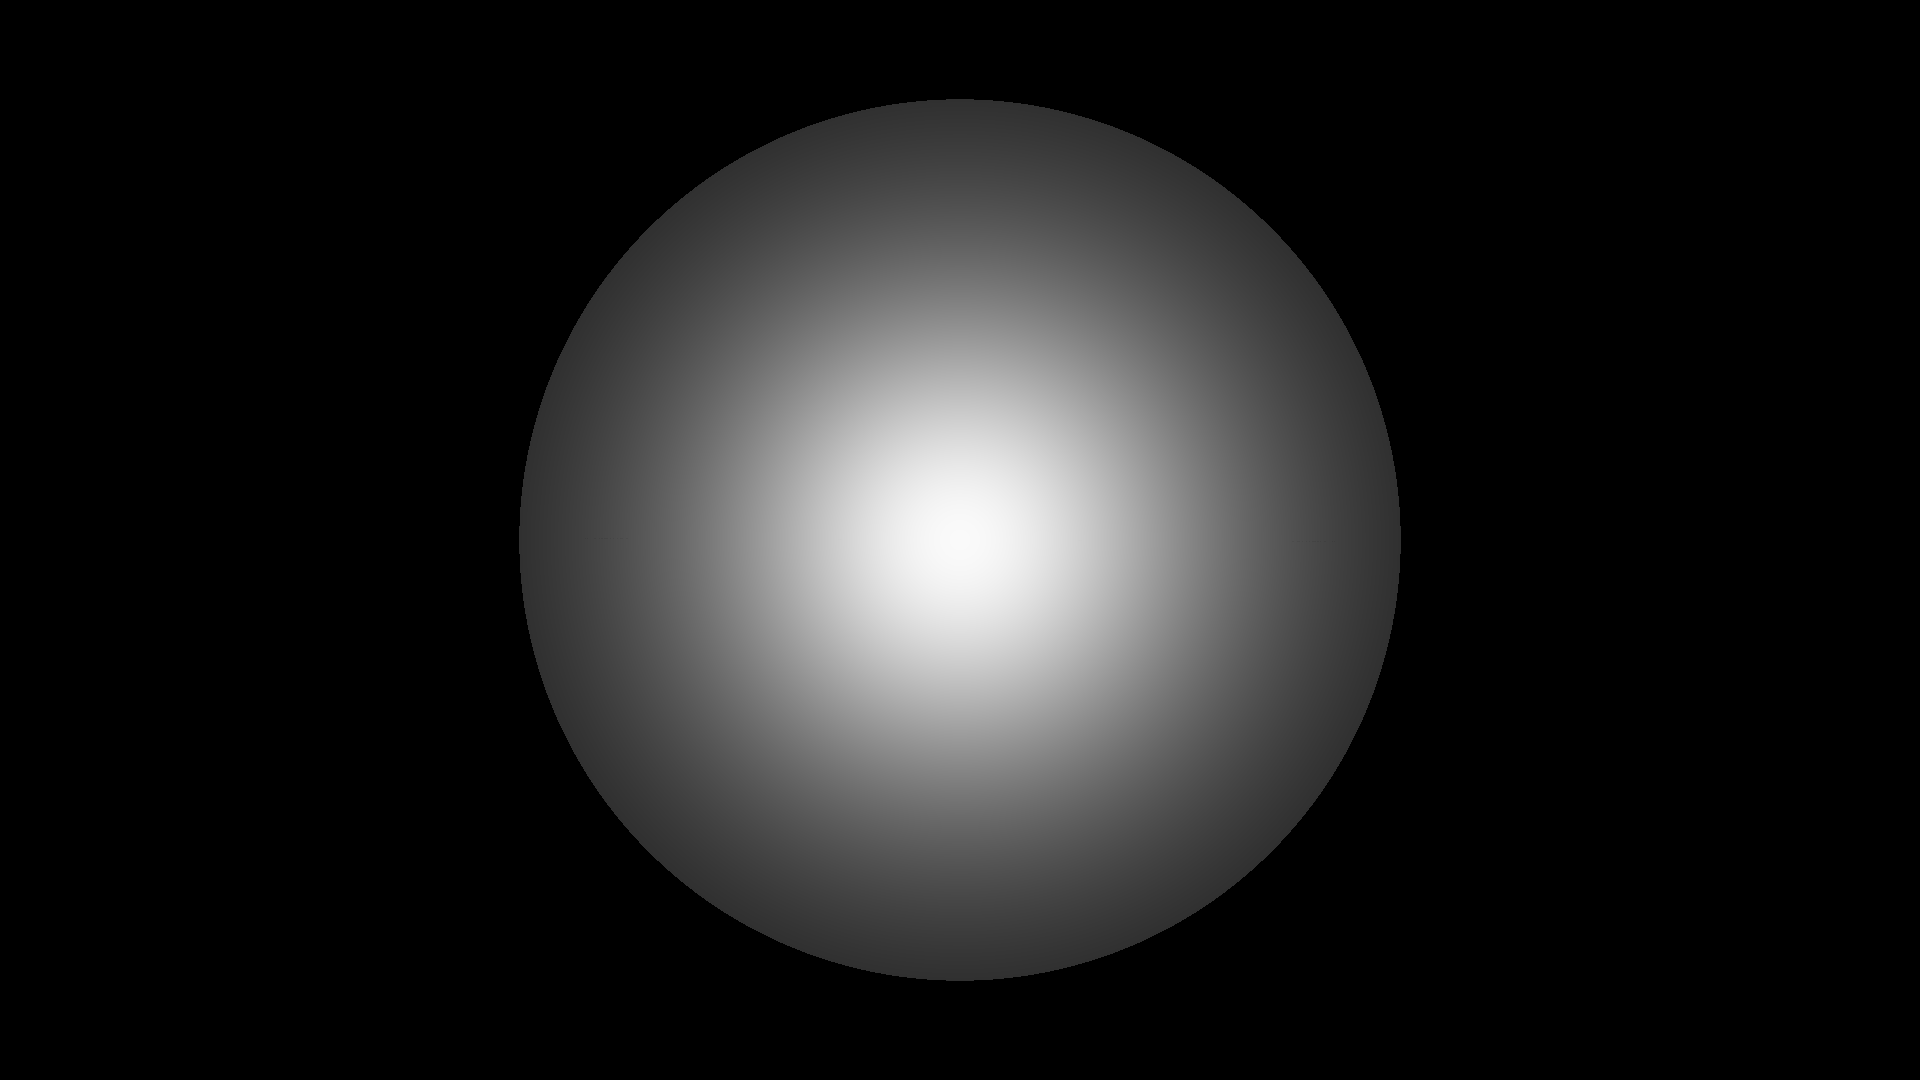
\includegraphics[width=0.3\textwidth]{chapters/ch3/img/light/output_07_07_0_0_1.png}}
\subfigure{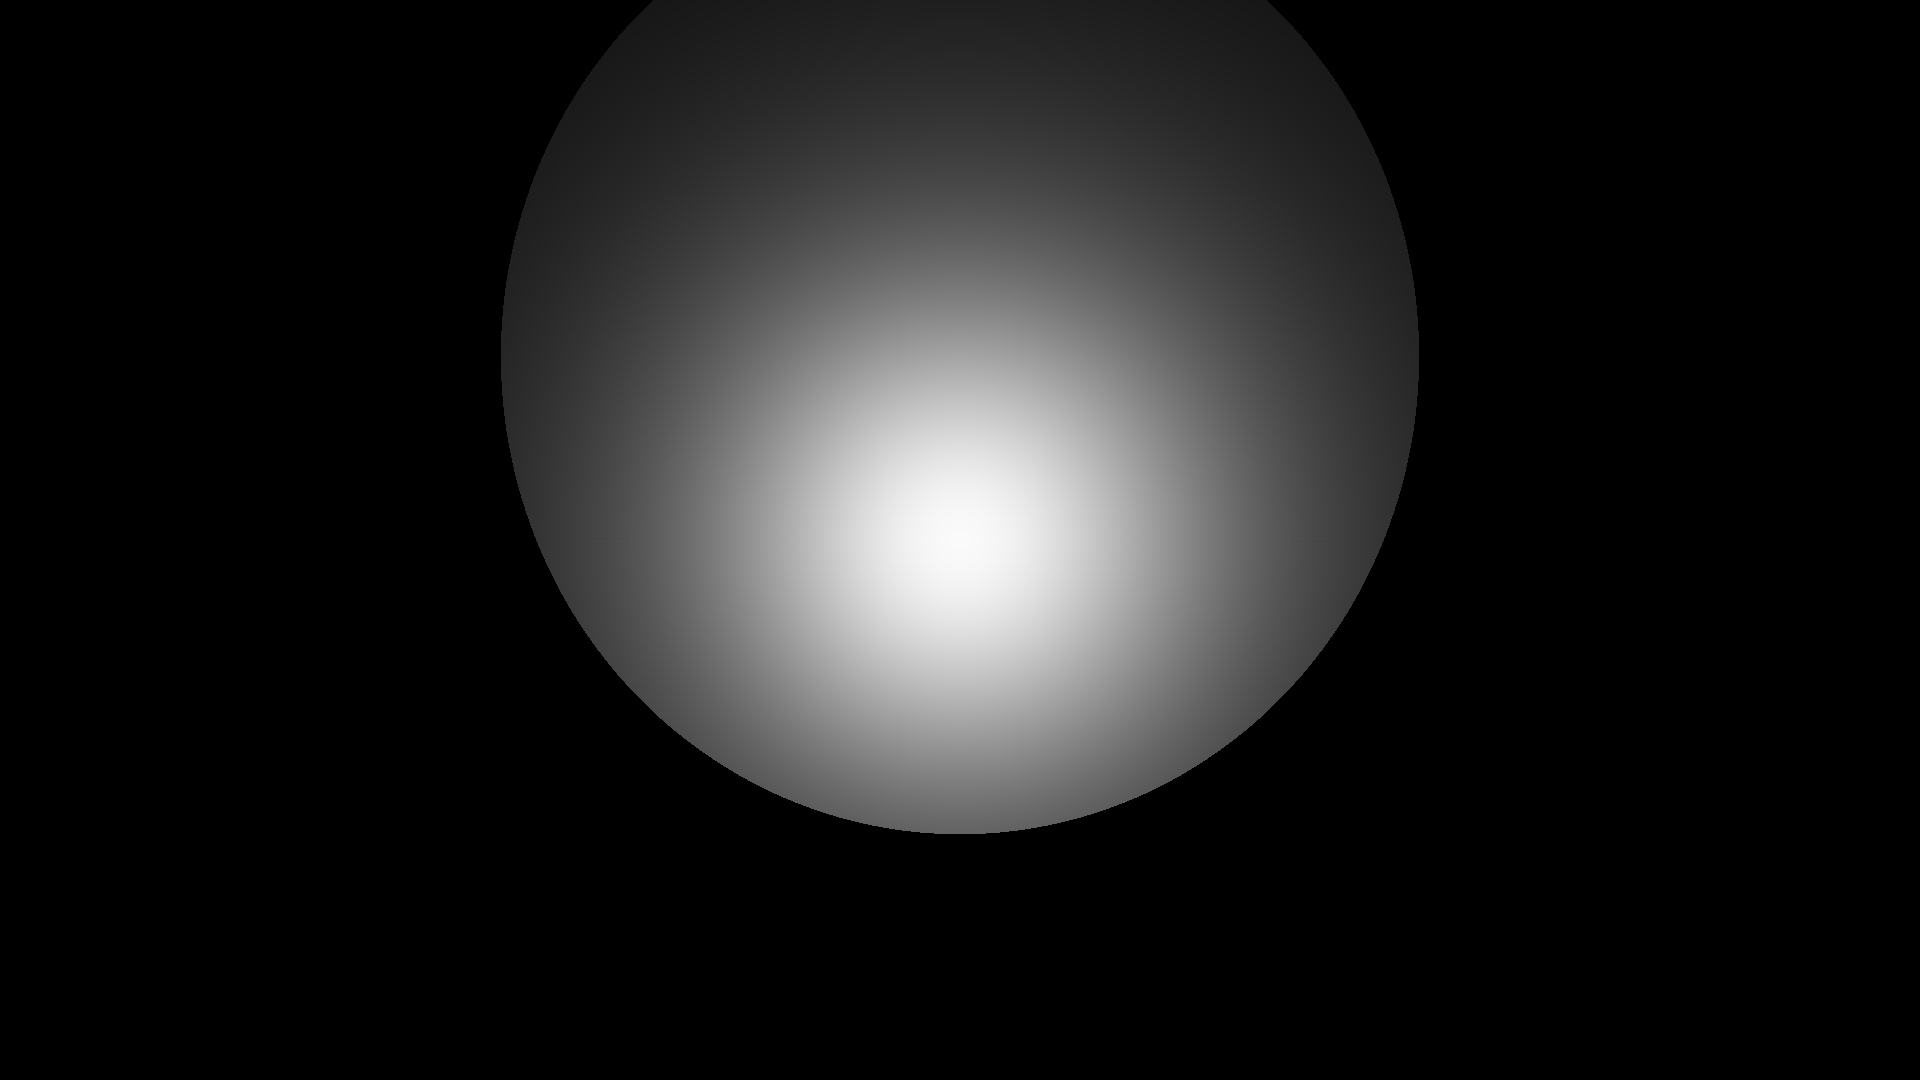
\includegraphics[width=0.3\textwidth]{chapters/ch3/img/light/output_07_07_0_02_1.png}}
\subfigure{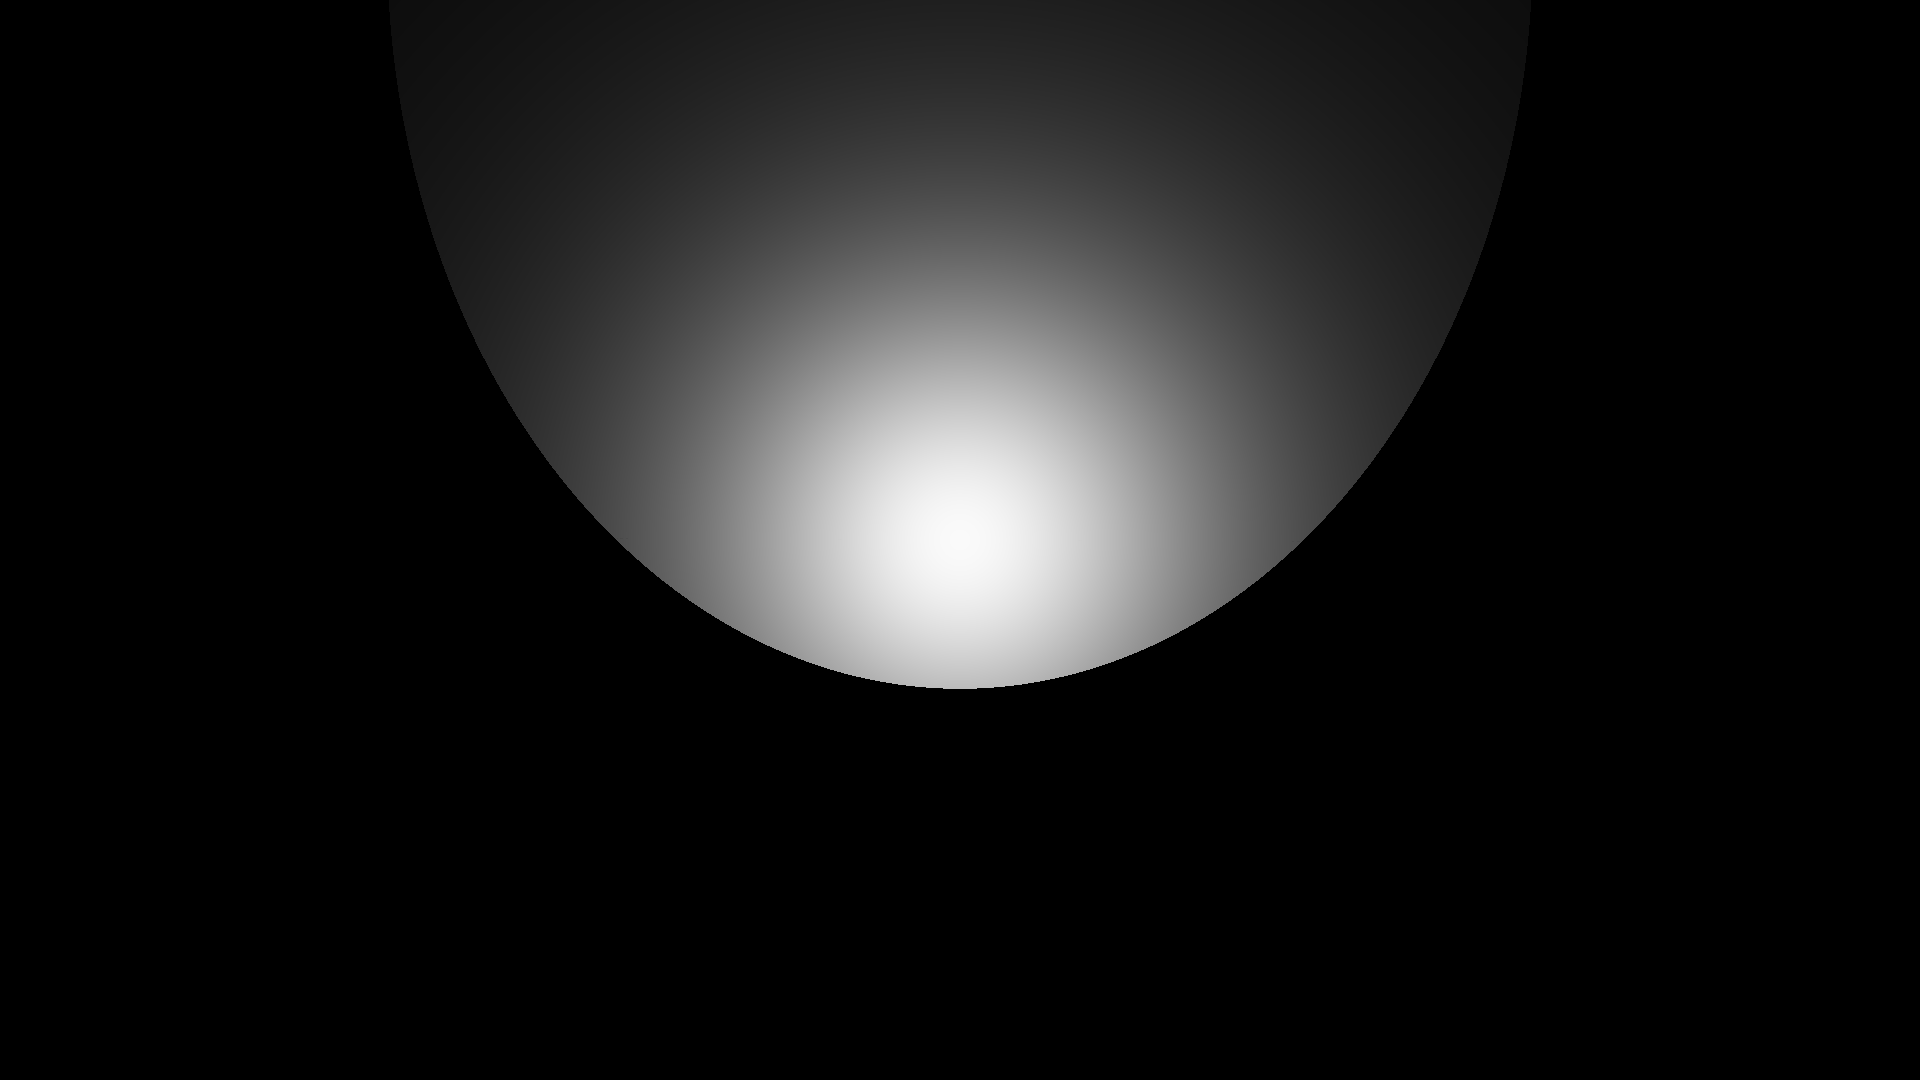
\includegraphics[width=0.3\textwidth]{chapters/ch3/img/light/output_07_07_0_05_1.png}}

\subfigure{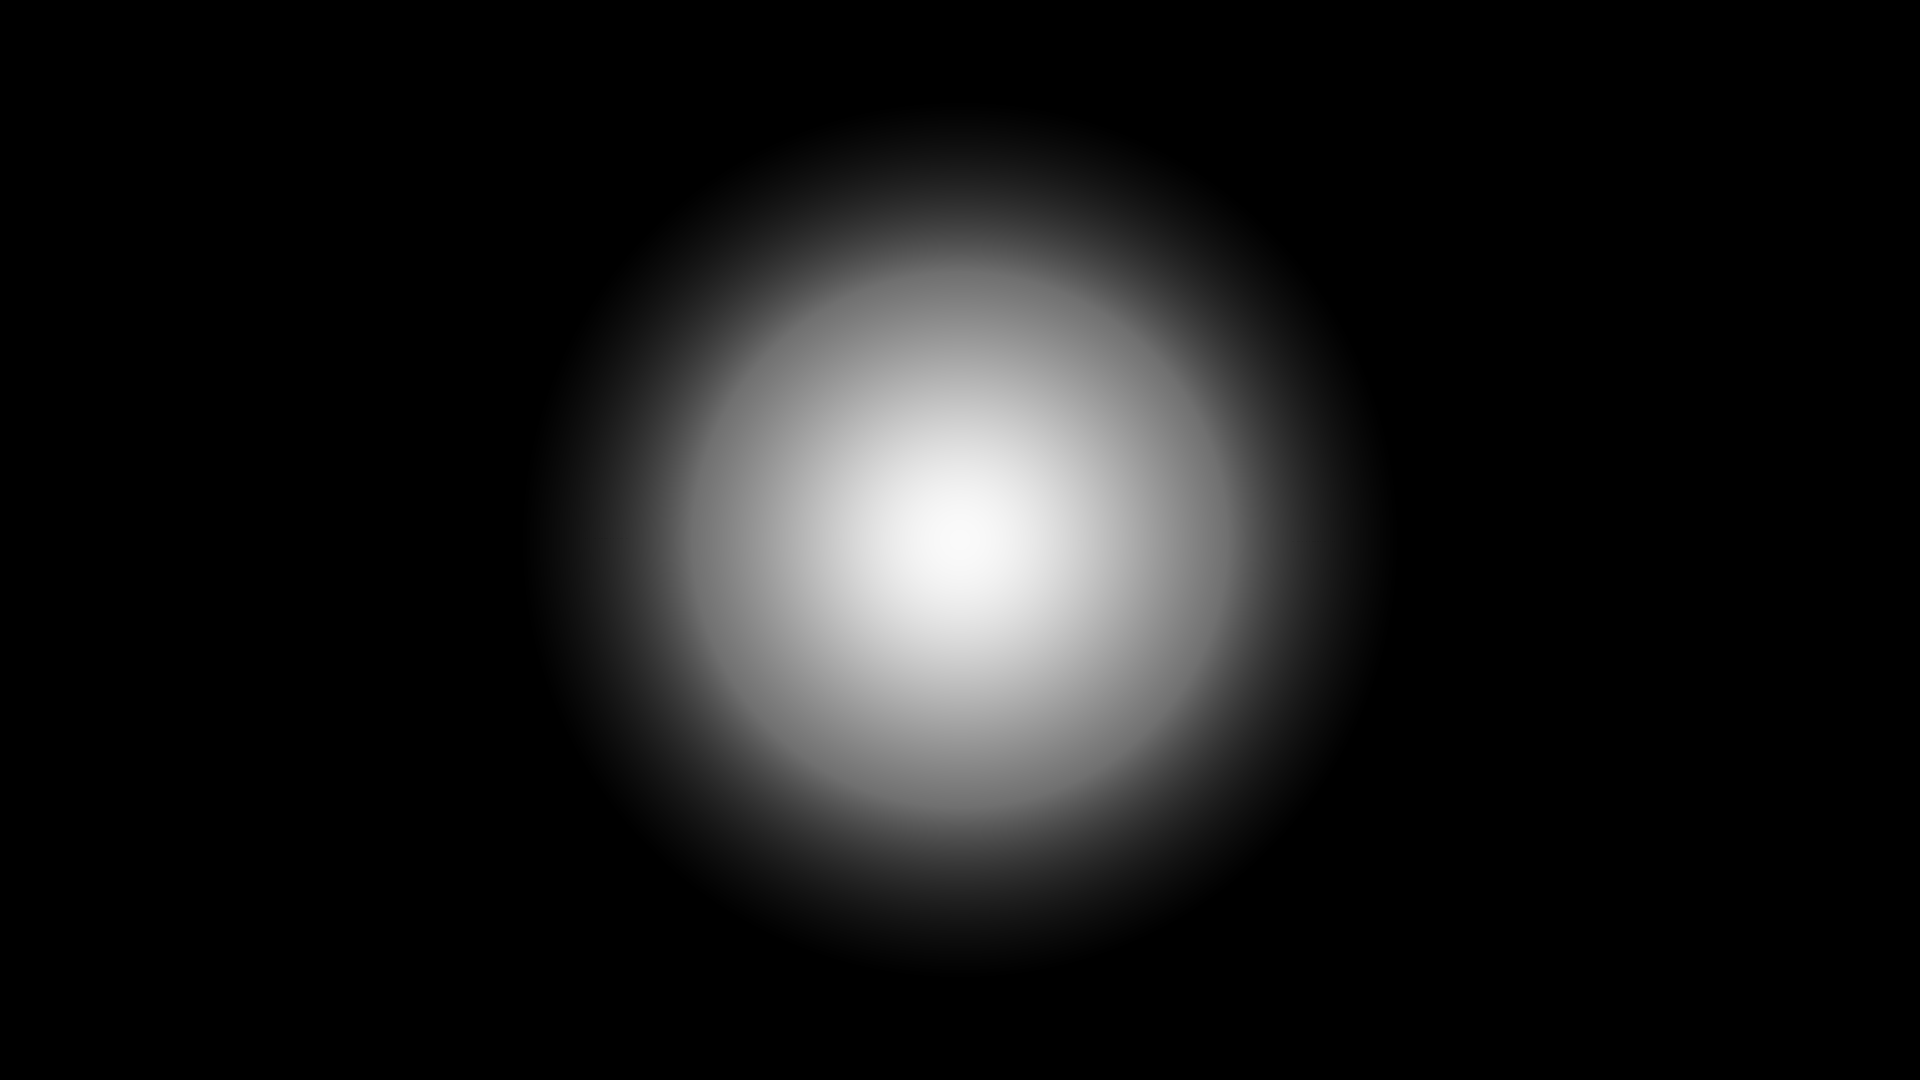
\includegraphics[width=0.3\textwidth]{chapters/ch3/img/light/output_07_085_0_0_1.png}}
\subfigure{
\includegraphics[width=0.3\textwidth]{chapters/ch3/img/light/output_07_085_0_02_1.png}}
\subfigure{
\includegraphics[width=0.3\textwidth]{chapters/ch3/img/light/output_07_085_0_05_1.png}}

\subfigure{
\includegraphics[width=0.3\textwidth]{chapters/ch3/img/light/output_07_1_0_0_1.png}}
\subfigure{
\includegraphics[width=0.3\textwidth]{chapters/ch3/img/light/output_07_1_0_02_1.png}}
\subfigure{
\includegraphics[width=0.3\textwidth]{chapters/ch3/img/light/output_07_1_0_05_1.png}}

\caption[Oświetlenie płaskiej powierzchni przez punktowe źródło światła]{Oświetlenie płaskiej powierzchni przez punktowe źródło światła. Obrazy w kolejnych kolumnach odpowiadają różnemu ustawieniu tego samego źródła względem płaszczyzny, zaś wiersze różnią się wartością $\cos\frac{\beta}{2}$ - idąc od góry 0,7; 0,85; 1,0 ($\cos\frac{\alpha}{2} = 0,7 = \mathrm{const}$). W przypadku, gdy $\cos\frac{\beta}{2}\neq\cos\frac{\alpha}{2}$, krawędź między obszarem oświetlonym a nieoświetlonym staje się rozmyta. Nieciągłości przejść między kolorami widoczne najbardziej w przypadku $\cos\frac{\beta}{2} = 0,85$ nie są wynikiem błędu algorytmu, a własności przetwarzania obrazu przez mózg człowieka - efekt ten zwany jest \textit{pasmami Macha}~\cite{MACH_BANDS}}
\label{ch3:img:light_comp}
\end{figure}

Część światła padającego na obiekt, zgodnie z równaniem~\eqref{ch3:eq:shading_equation_general} może się na nim rozproszyć lub odbić w sposób zwierciadlany\footnote{Przypadek kierunkowego odbicia rozproszonego nie jest rozpatrywany przez \textsc{ViRay}.}. W pierwszym przypadku rozproszenie to jest przybliżane przez model Orena-Nayara~\eqref{ch1:eq:ON_BRDF}, którego przypadkiem granicznym, gdy $\sigma^2 = 0$, jest model Lamberta~\eqref{ch1:eq:LambertBRDF}. Wpływ parametru szorstkości $\sigma^2$ na oświetlenie powierzchni został zobrazowany na rysunku~\ref{ch3:img:diffuse_params}. Na jego podstawie można stwierdzić, iż wraz ze wzrostem $\sigma^2$ rozkład oświetlenia staje się bardziej równomierny, a maksimum jasności ma mniejszą wartość. 

\begin{figure}[H]
\centering
\subfigure{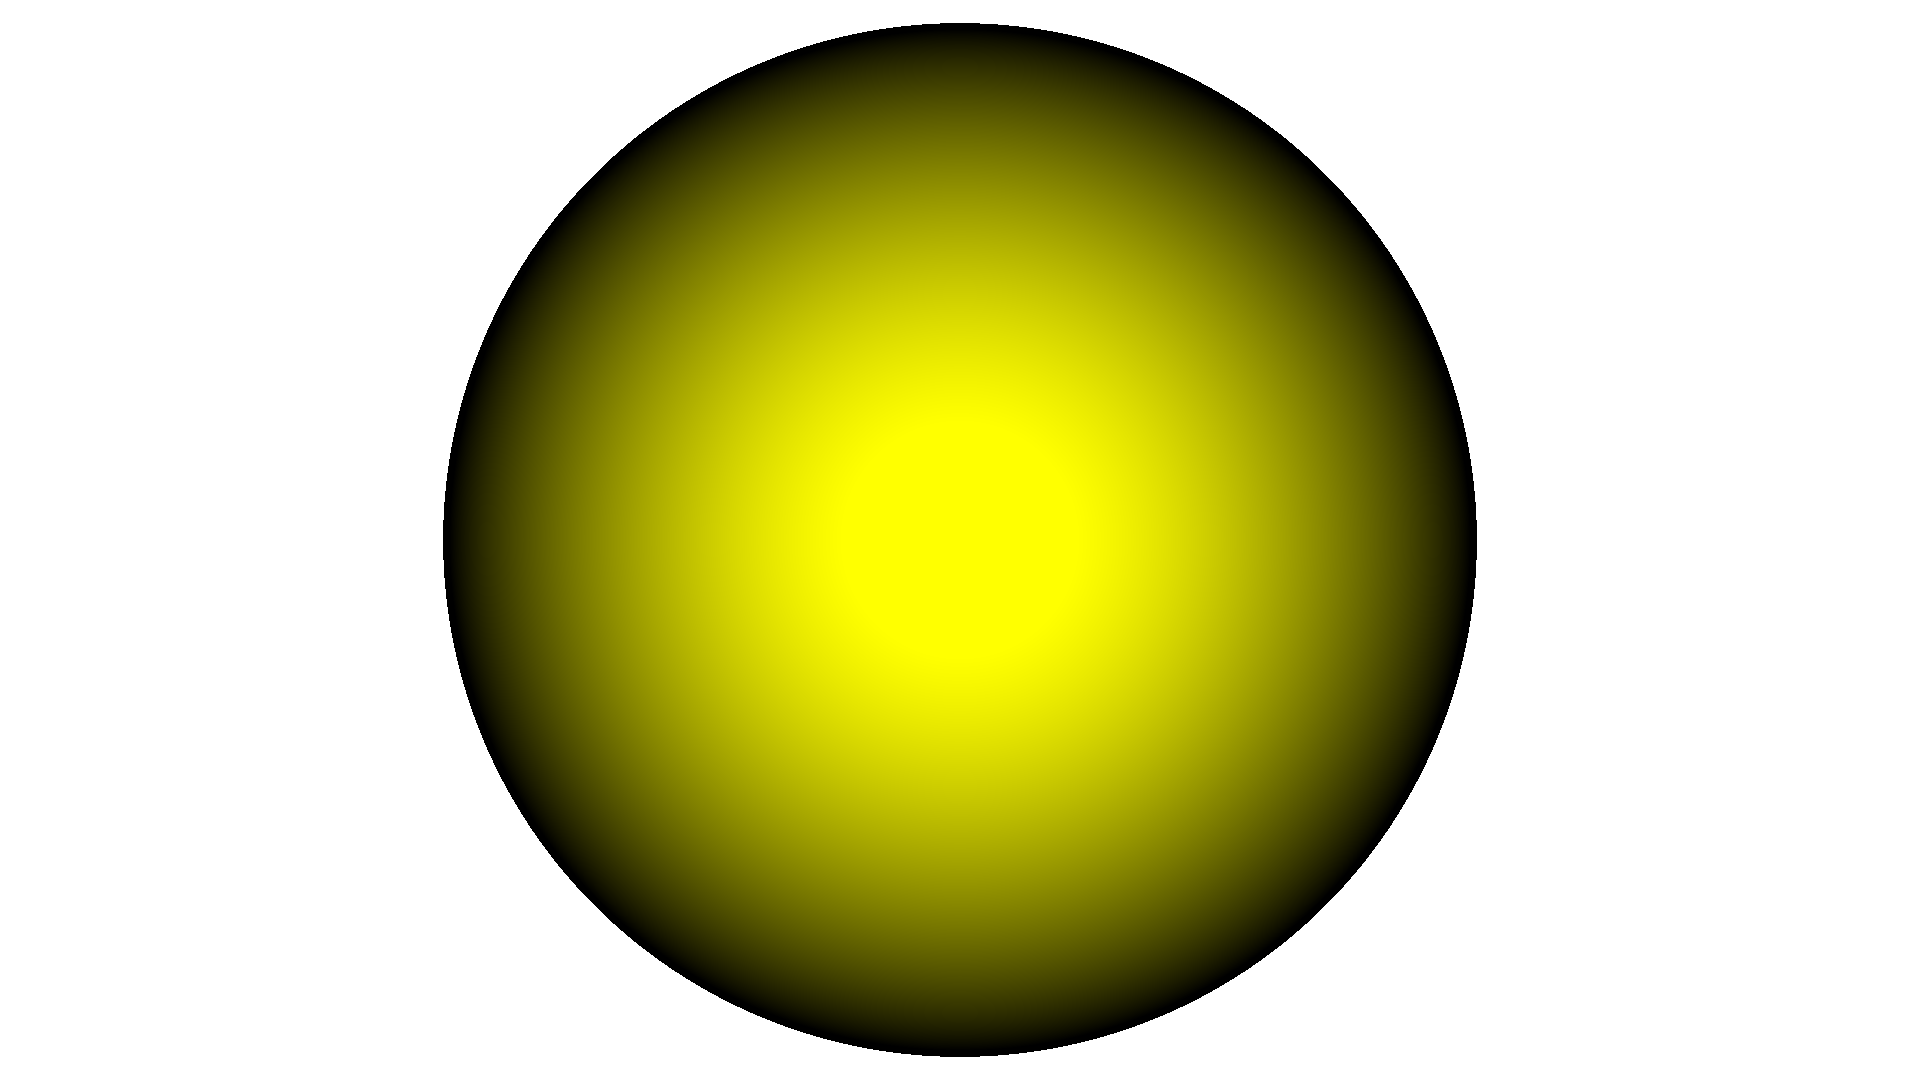
\includegraphics[width=0.3\textwidth]{chapters/ch3/img/diffuse/direct_0.png}}
\subfigure{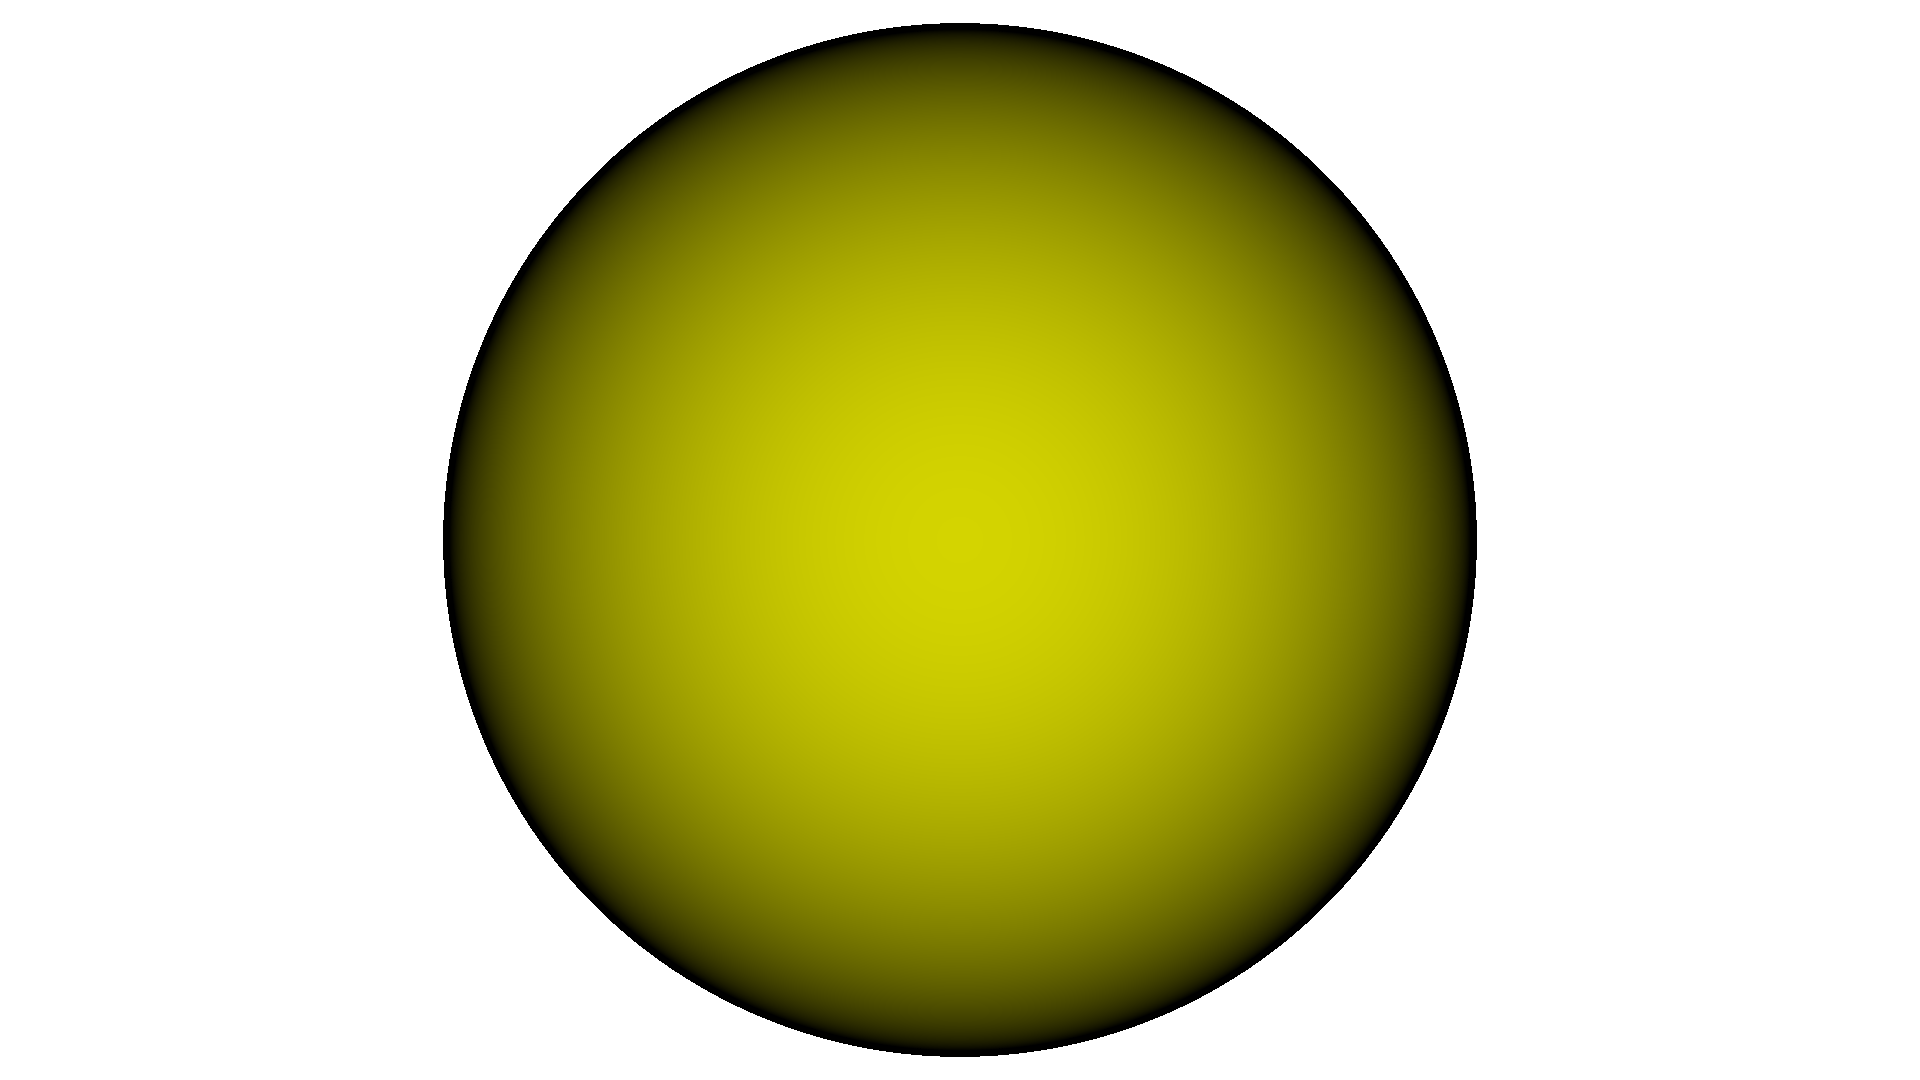
\includegraphics[width=0.3\textwidth]{chapters/ch3/img/diffuse/direct_025.png}}
\subfigure{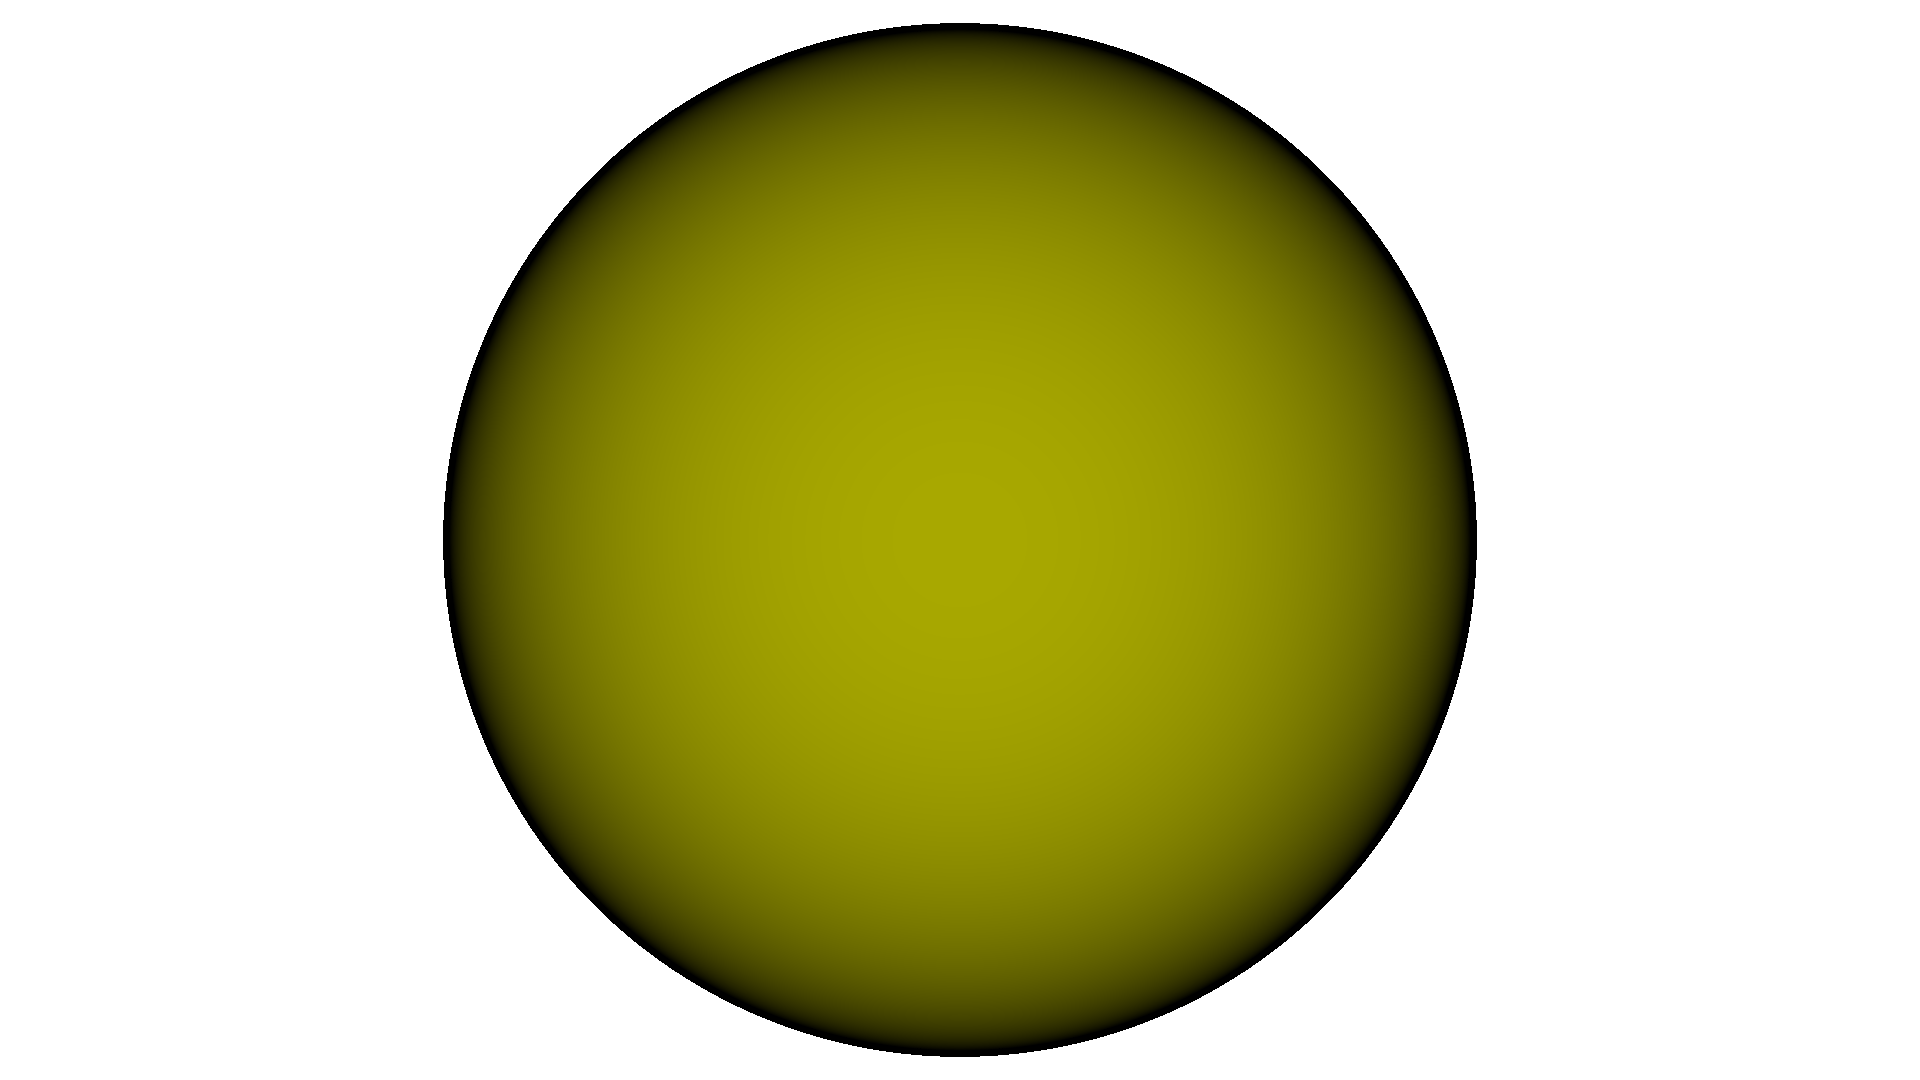
\includegraphics[width=0.3\textwidth]{chapters/ch3/img/diffuse/direct_1.png}}

\subfigure{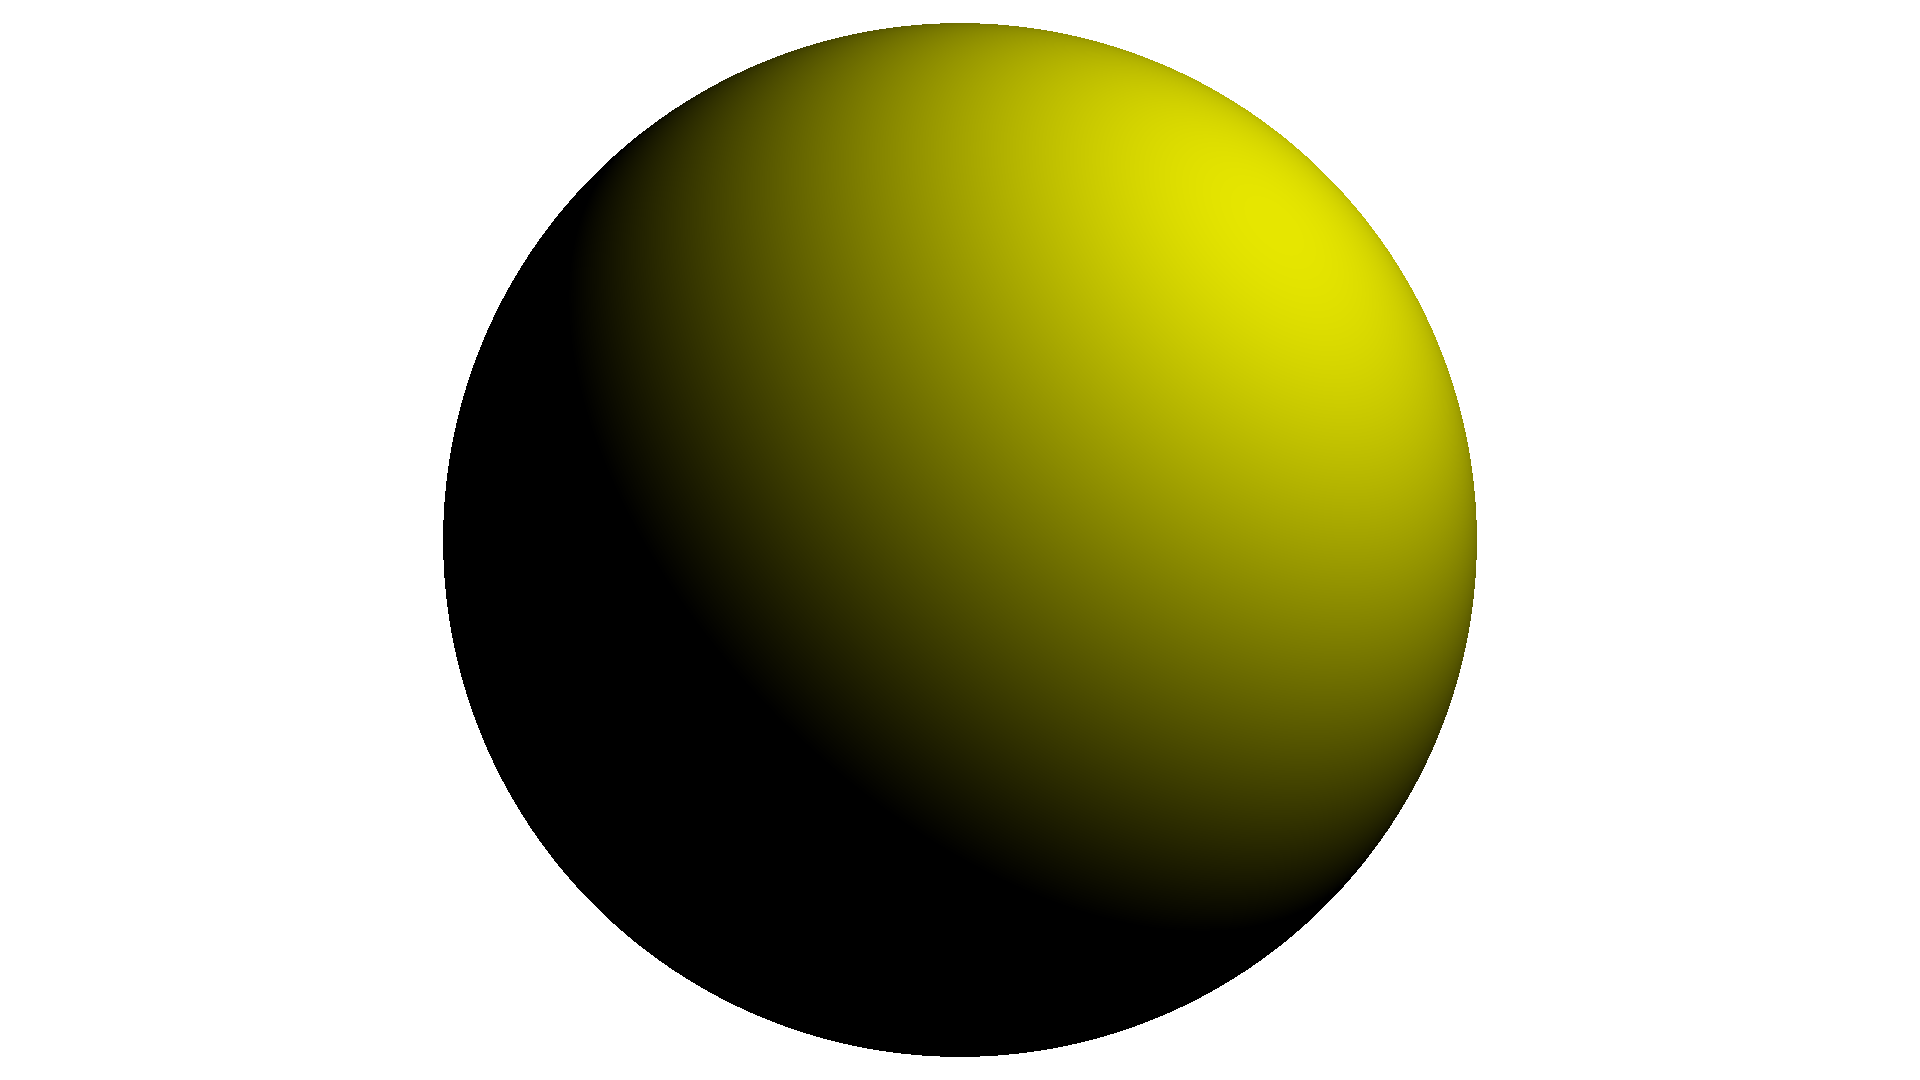
\includegraphics[width=0.3\textwidth]{chapters/ch3/img/diffuse/angle_0.png}}
\subfigure{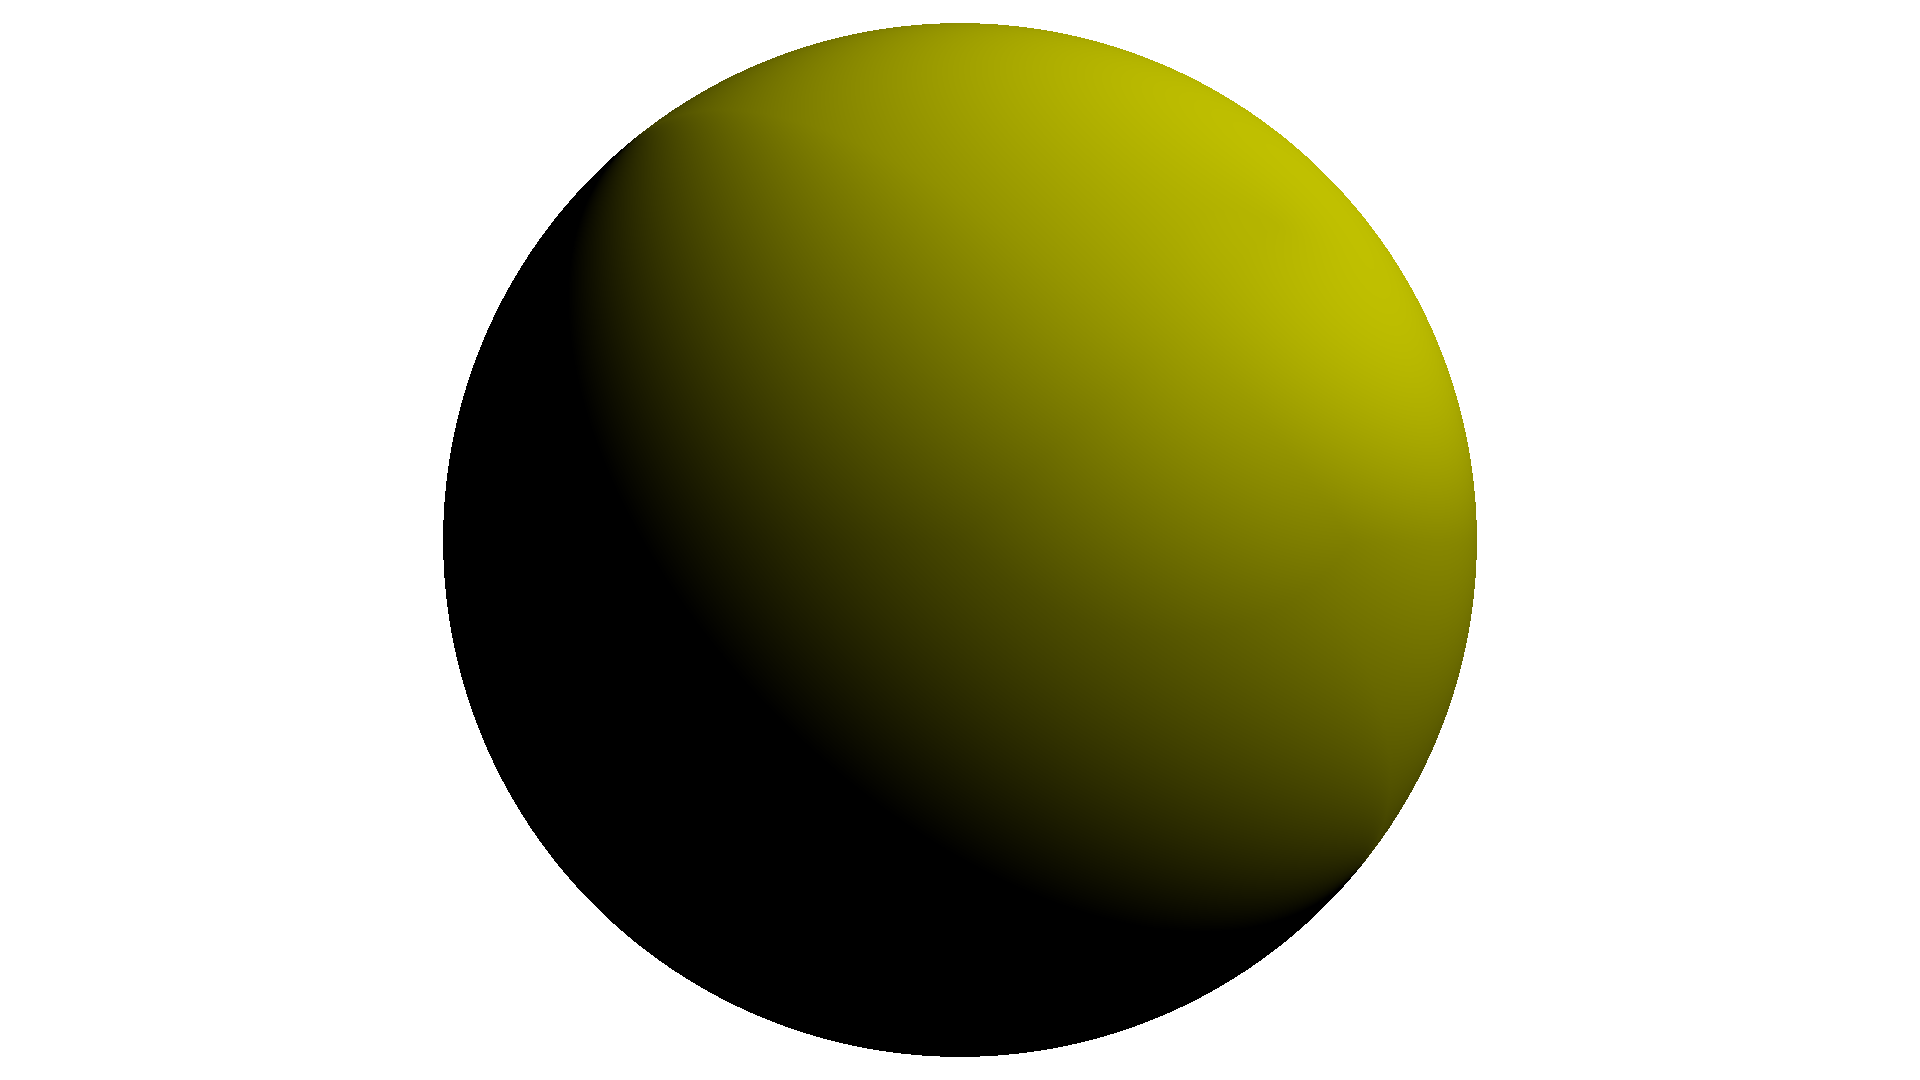
\includegraphics[width=0.3\textwidth]{chapters/ch3/img/diffuse/angle_025.png}}
\subfigure{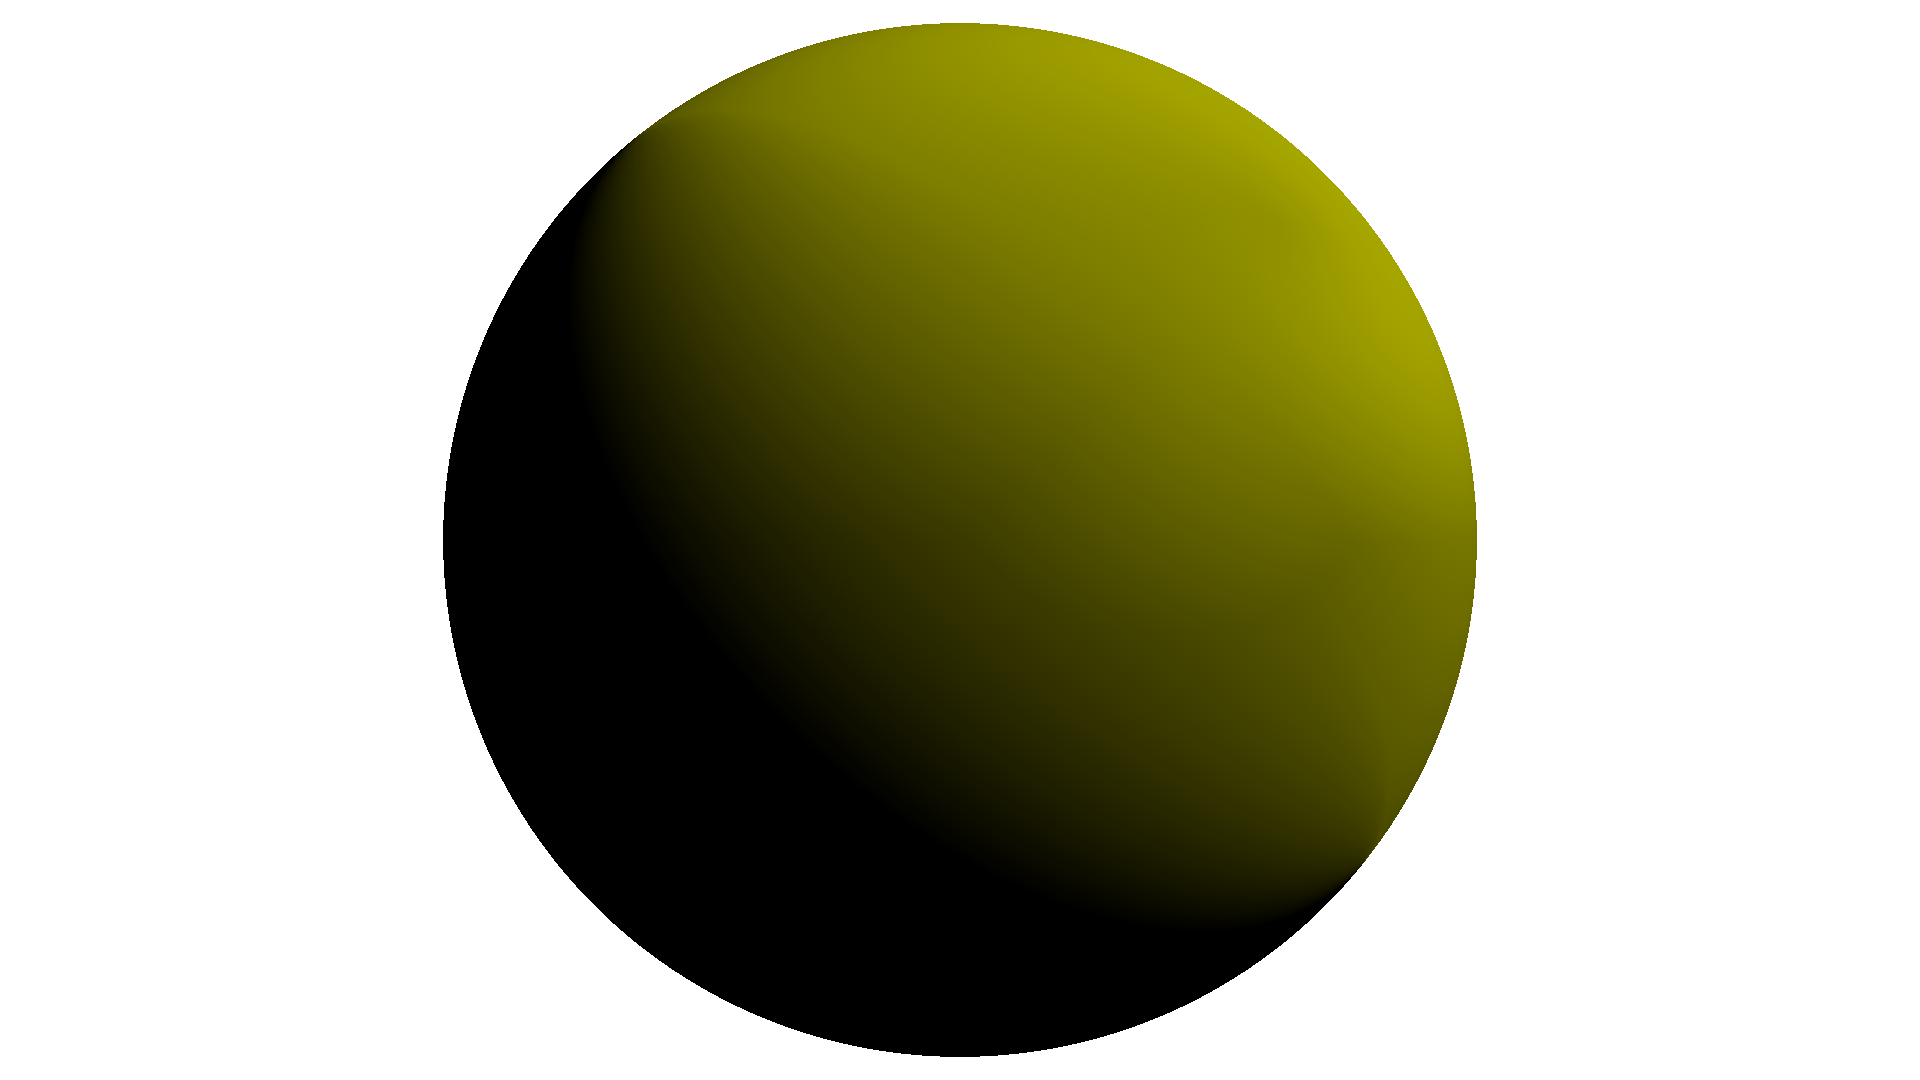
\includegraphics[width=0.3\textwidth]{chapters/ch3/img/diffuse/angle_1.png}}

\caption[Oświetlenie powierzchni odbijającej światło całkowicie w sposób rozproszony zgodnie z modelem Orena-Nayara]{Oświetlenie powierzchni odbijającej światło całkowicie w sposób rozproszony zgodnie z modelem Orena-Nayara. Górny wiersz odpowiada sytuacji, gdy kierunek obserwacji $\vec{d}$ oraz kierunek światła $\overrightarrow{l_{dir}}$ są identyczne i przechodzą przez środek oświetlanej kuli. W~dolnym wierszu wspomniane kierunki nie pokrywają się. Kolejne kolumny~(od lewej do prawej) odpowiadają różnym wartościom współczynnika szorstkości materiału $\sigma^2\in\lbrace 0; 0,25; 1 \rbrace$, wraz ze wzrostem którego następuje coraz większe zrównanie jasności oświetlanej powierzchni}
\label{ch3:img:diffuse_params}
\end{figure}

Drugim z komponentów oświetlenia jest odbicie zwierciadlane, które w \textsc{ViRay}'u można modelować za pomocą modelu Blinna-Phonga~\eqref{ch1:eq:PhongBRDFNormalized} bądź też Torrance'a-Sparrowa~\eqref{ch1:eq:TorranceSparrowFull}. Decyzja o rezygnacji z modelu Phonga na rzecz Blinna-Phonga podyktowana została tym, że model Blinna-Phonga oraz Torrance'a-Sparrowa współdzielą ze sobą obliczenia związane z czynnikiem rozkładu orientacji mikrościanek wokół wektora połówkowego $D(\vec{\omega_h})$~\eqref{ch1:eq:TorranceSparrow_D}, przez co implementacja tego pierwszego nie wiąże się z wykorzystaniem dodatkowych zasobów układu FPGA. Wpływ parametru skupienia rozbłysku $e \in \mathbb{N}$ w~modelu Blinna-Phonga został zaprezentowany na przykładzie oświetlenia powierzchni walcowej~(rysunek~\ref{ch3:img:blinn_phong}).
\begin{figure}[H]
\centering
\subfigure{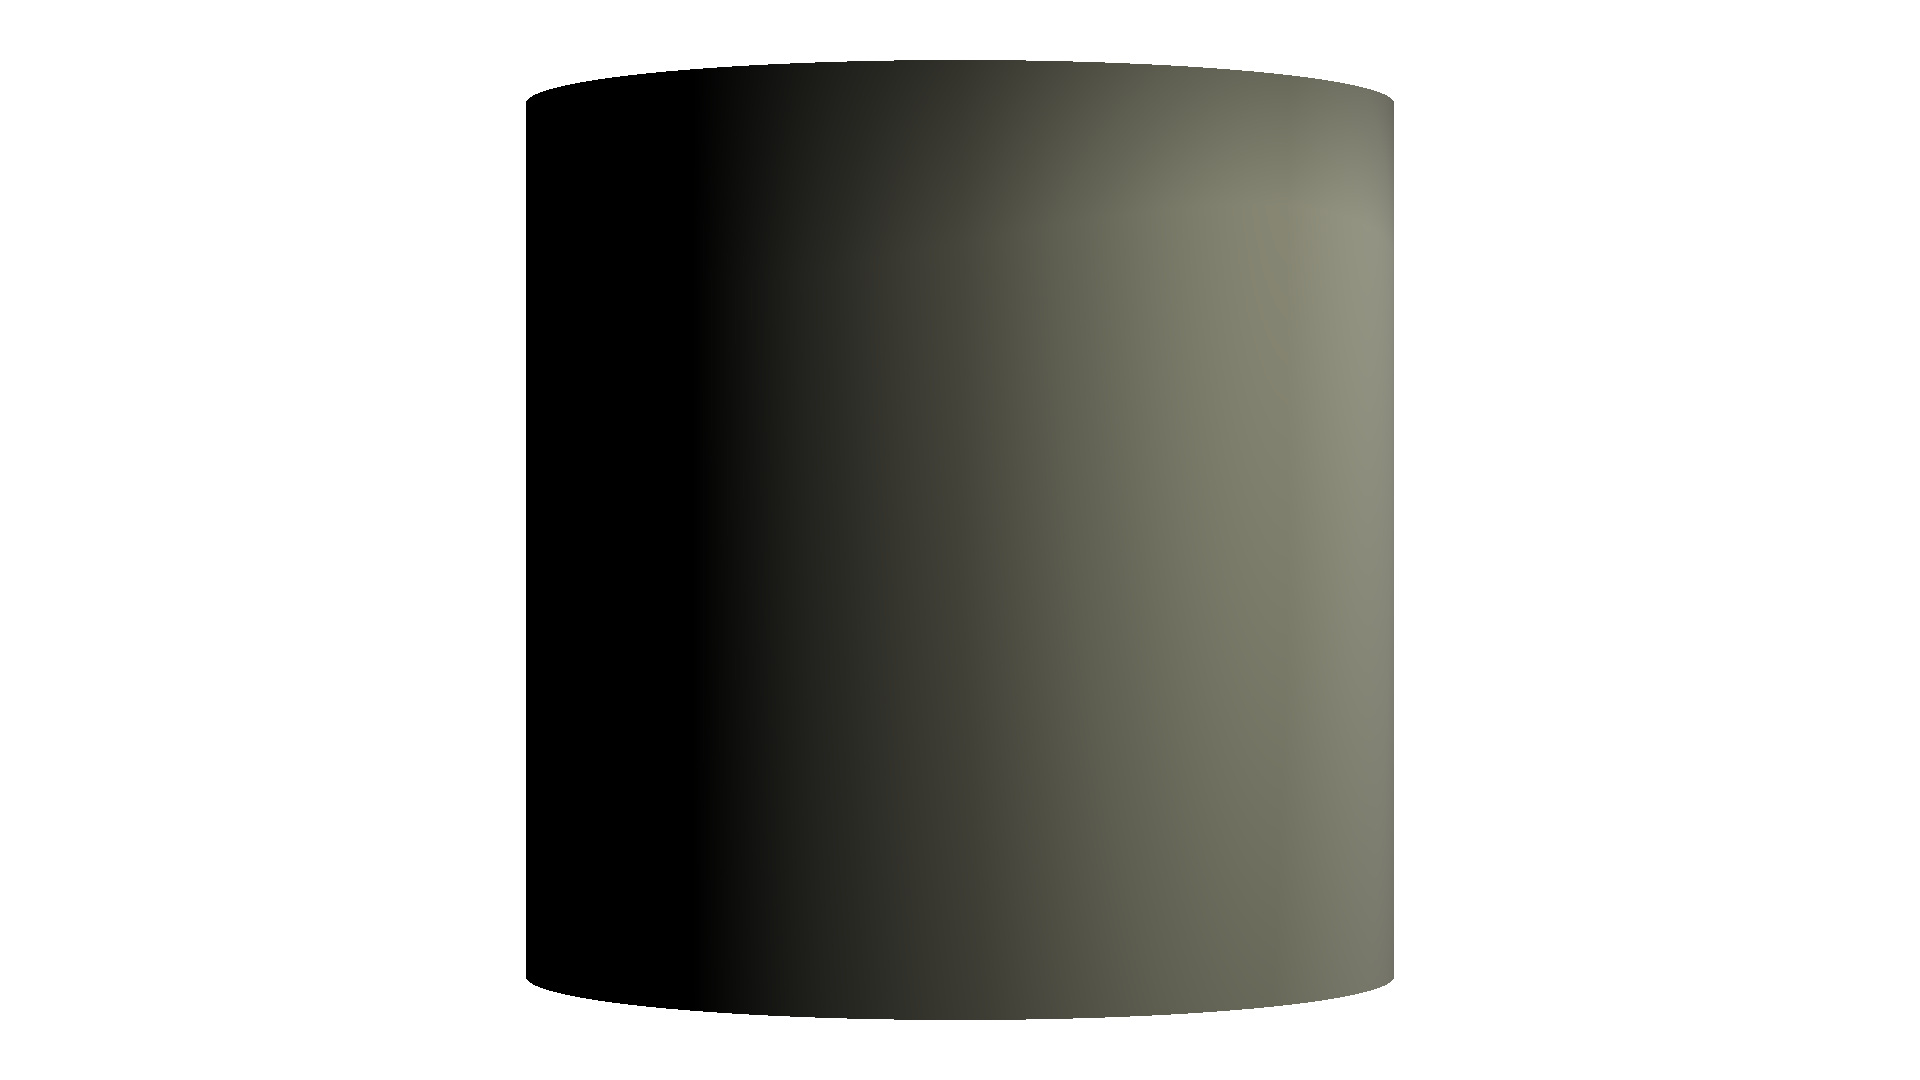
\includegraphics[width=0.45\textwidth]{chapters/ch3/img/BlinnPhong/BP0.png}}
\subfigure{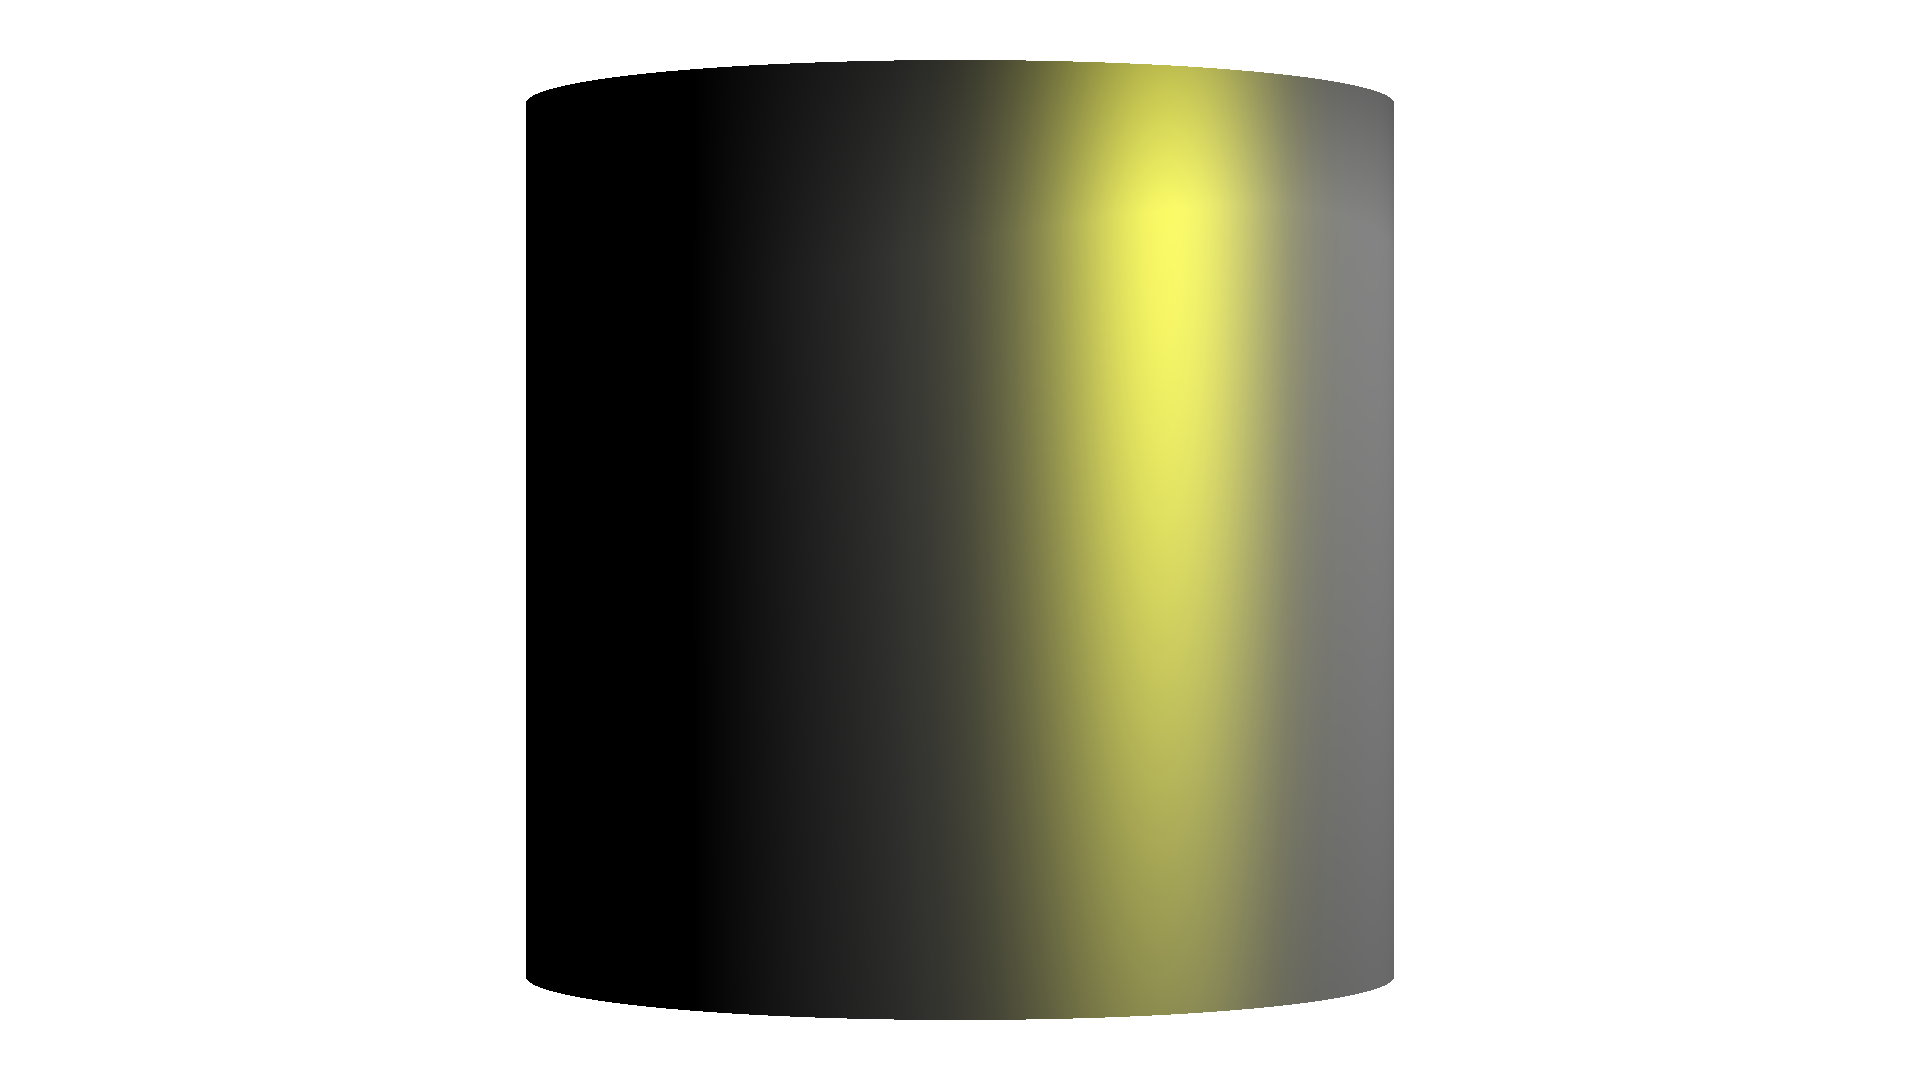
\includegraphics[width=0.45\textwidth]{chapters/ch3/img/BlinnPhong/BP16.png}}
\subfigure{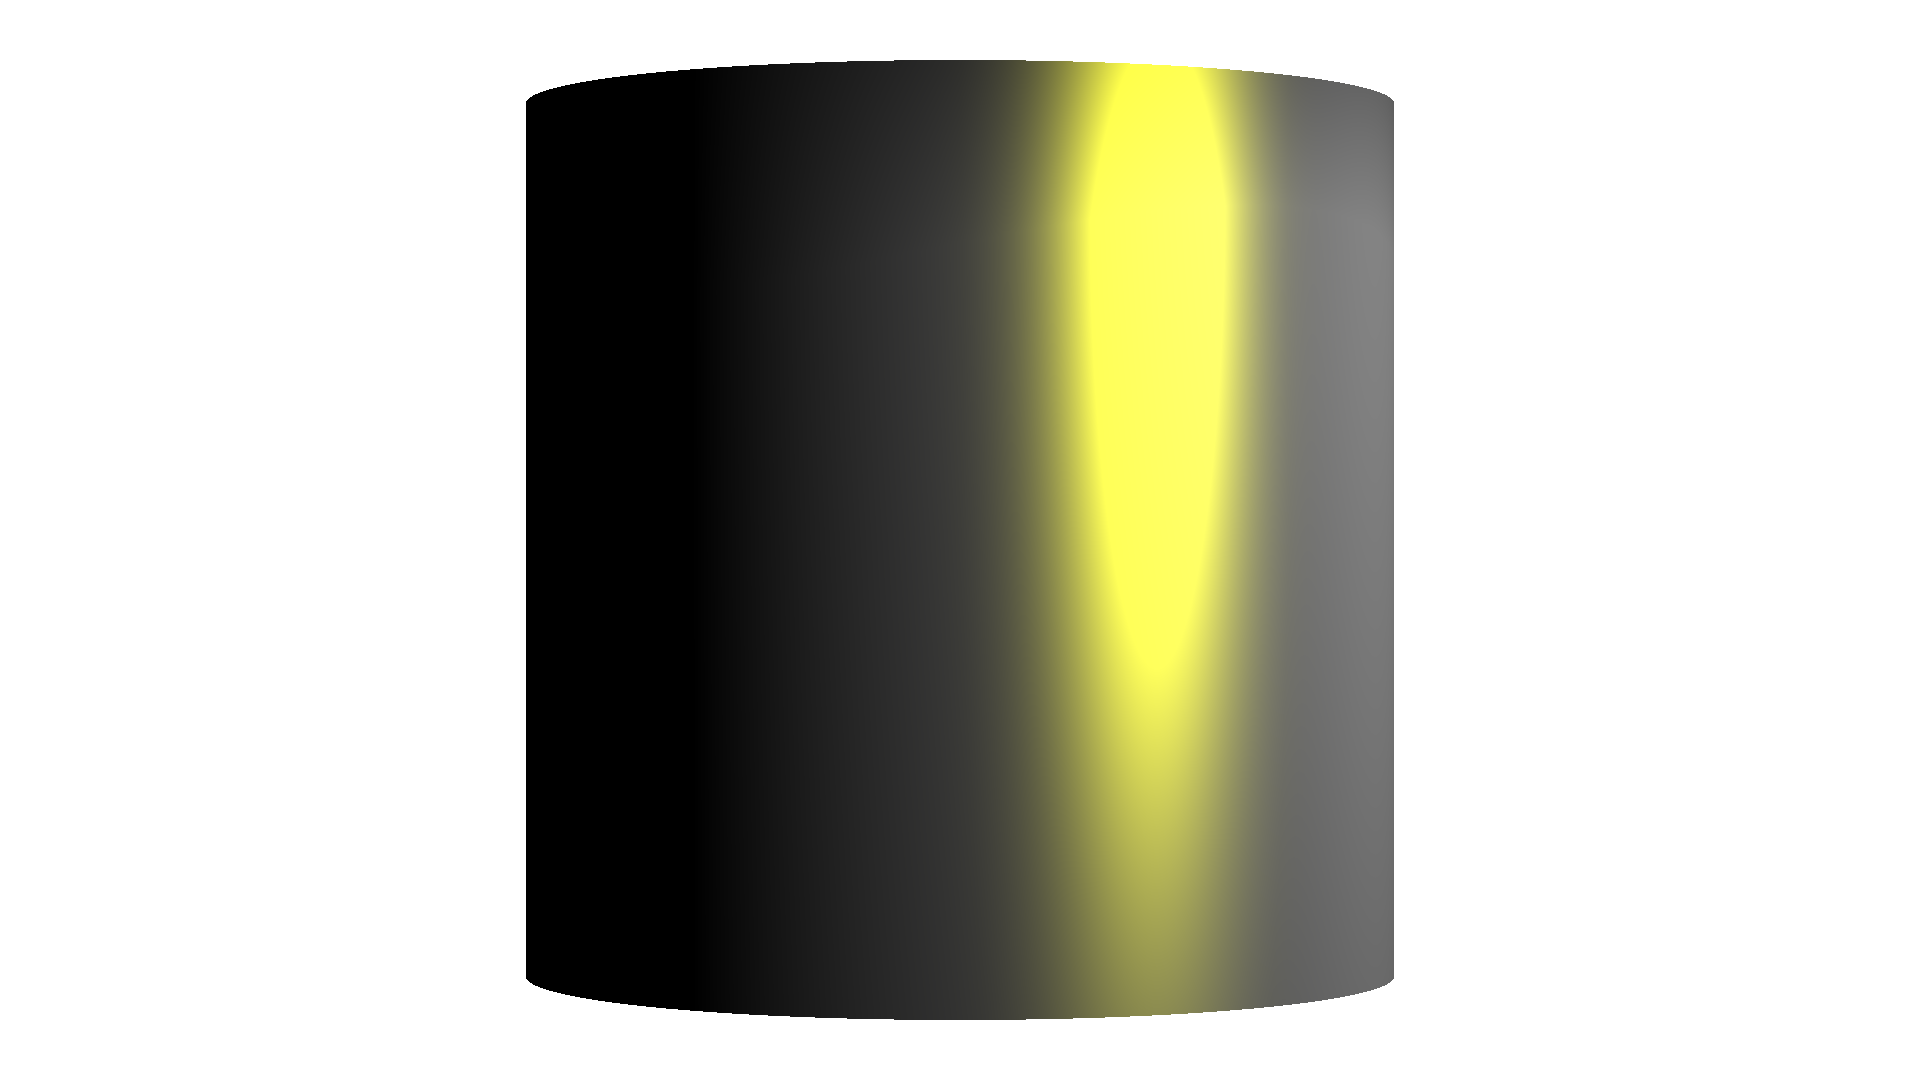
\includegraphics[width=0.45\textwidth]{chapters/ch3/img/BlinnPhong/BP32.png}}
\subfigure{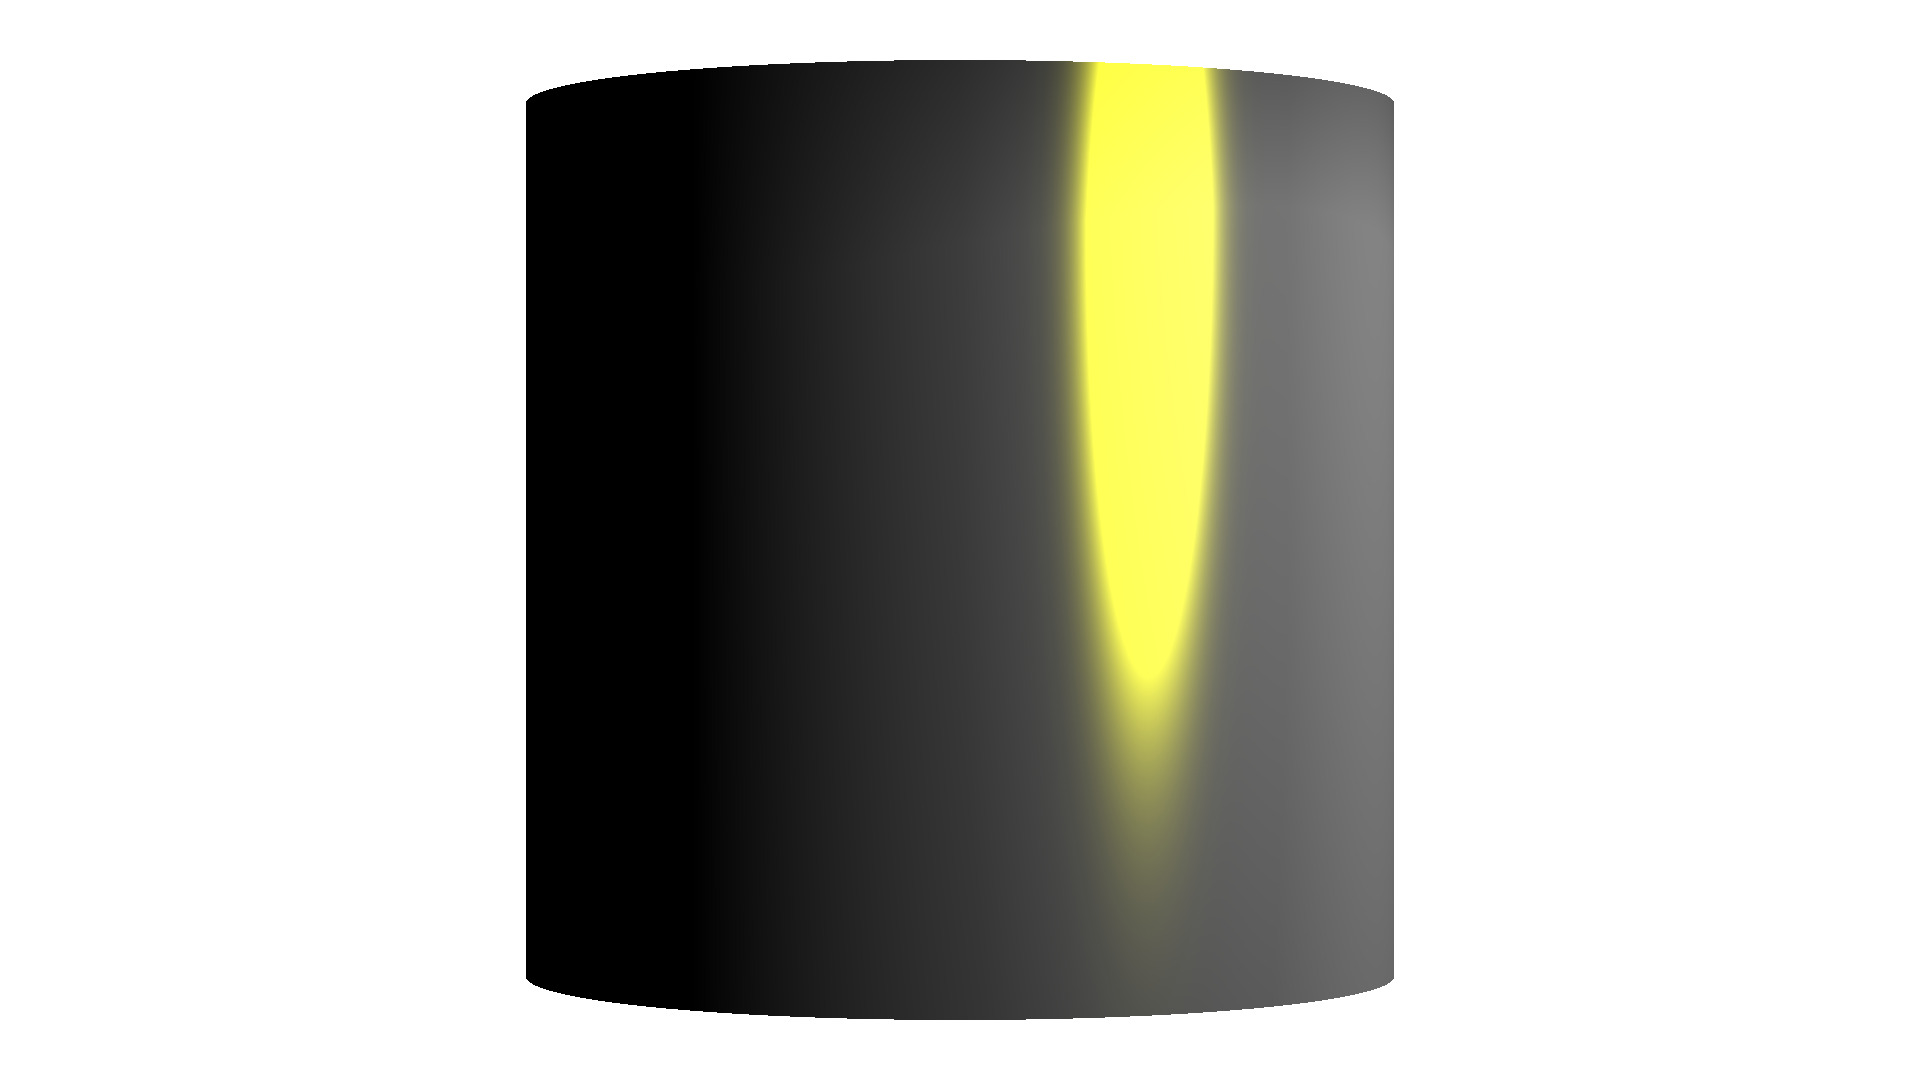
\includegraphics[width=0.45\textwidth]{chapters/ch3/img/BlinnPhong/BP128.png}}

\caption[Rola parametru rozbłysku $e$ w modelu Blinna-Phonga]{Rola parametru rozbłysku $e$ w modelu Blinna-Phonga. Idąc od lewej do prawej z góry na dół parametr $e$ przyjmuje następujące wartości: 0, 16, 32, 128. Z uwagi na fakt, iż~kolory zapisywane są w postaci 24-bitowych wartości, gdzie każda z trzech składowych \texttt{RGB} reprezentowana jest przez 8 bitów, na obrazach dostrzec można efekty związane z obcięciem wartości do 255, które objawiają się jako obszary rozbłysku o jednakowym kolorze.}
\label{ch3:img:blinn_phong}
\end{figure}

Analizę działania modelu Torrance'a-Sparrowa najłatwiej dokonać w połączeniu ze sprawdzeniem, jak różne wartości współczynnika załamania $\eta$~(oraz absorpcji $k$ dla przewodników) wpływają na zdolność odbijania promieni od powierzchni. Bierze się to z faktu, iż model Torrance'a-Sparrowa ingeruje bezpośrednio w wartość współczynnika odbicia $r_{l-1}$, który zależy tu od przestrzennej relacji między wektorem połówkowym $\vec{\omega_h}$ a kątem $\vec{\omega_o}$~(w przeciwieństwie do typowej zależności między wektorem normalnym $\vec{n}$ a $\vec{\omega_o}$).

Poniższe obrazy uzyskano dla wartości współczynnika skupienia $e=128$ dla modelu Blinna-Phonga oraz $e=1024$ w przypadku modelu Torrance'a-Sparrowa - różnica ta opiera się na obserwacji, że model Torrance'a-Sparrowa generuje znacznie słabsze rozbłyski, dla takich samych wartości $e$.

\begin{figure}[H]
\centering
\subfigure{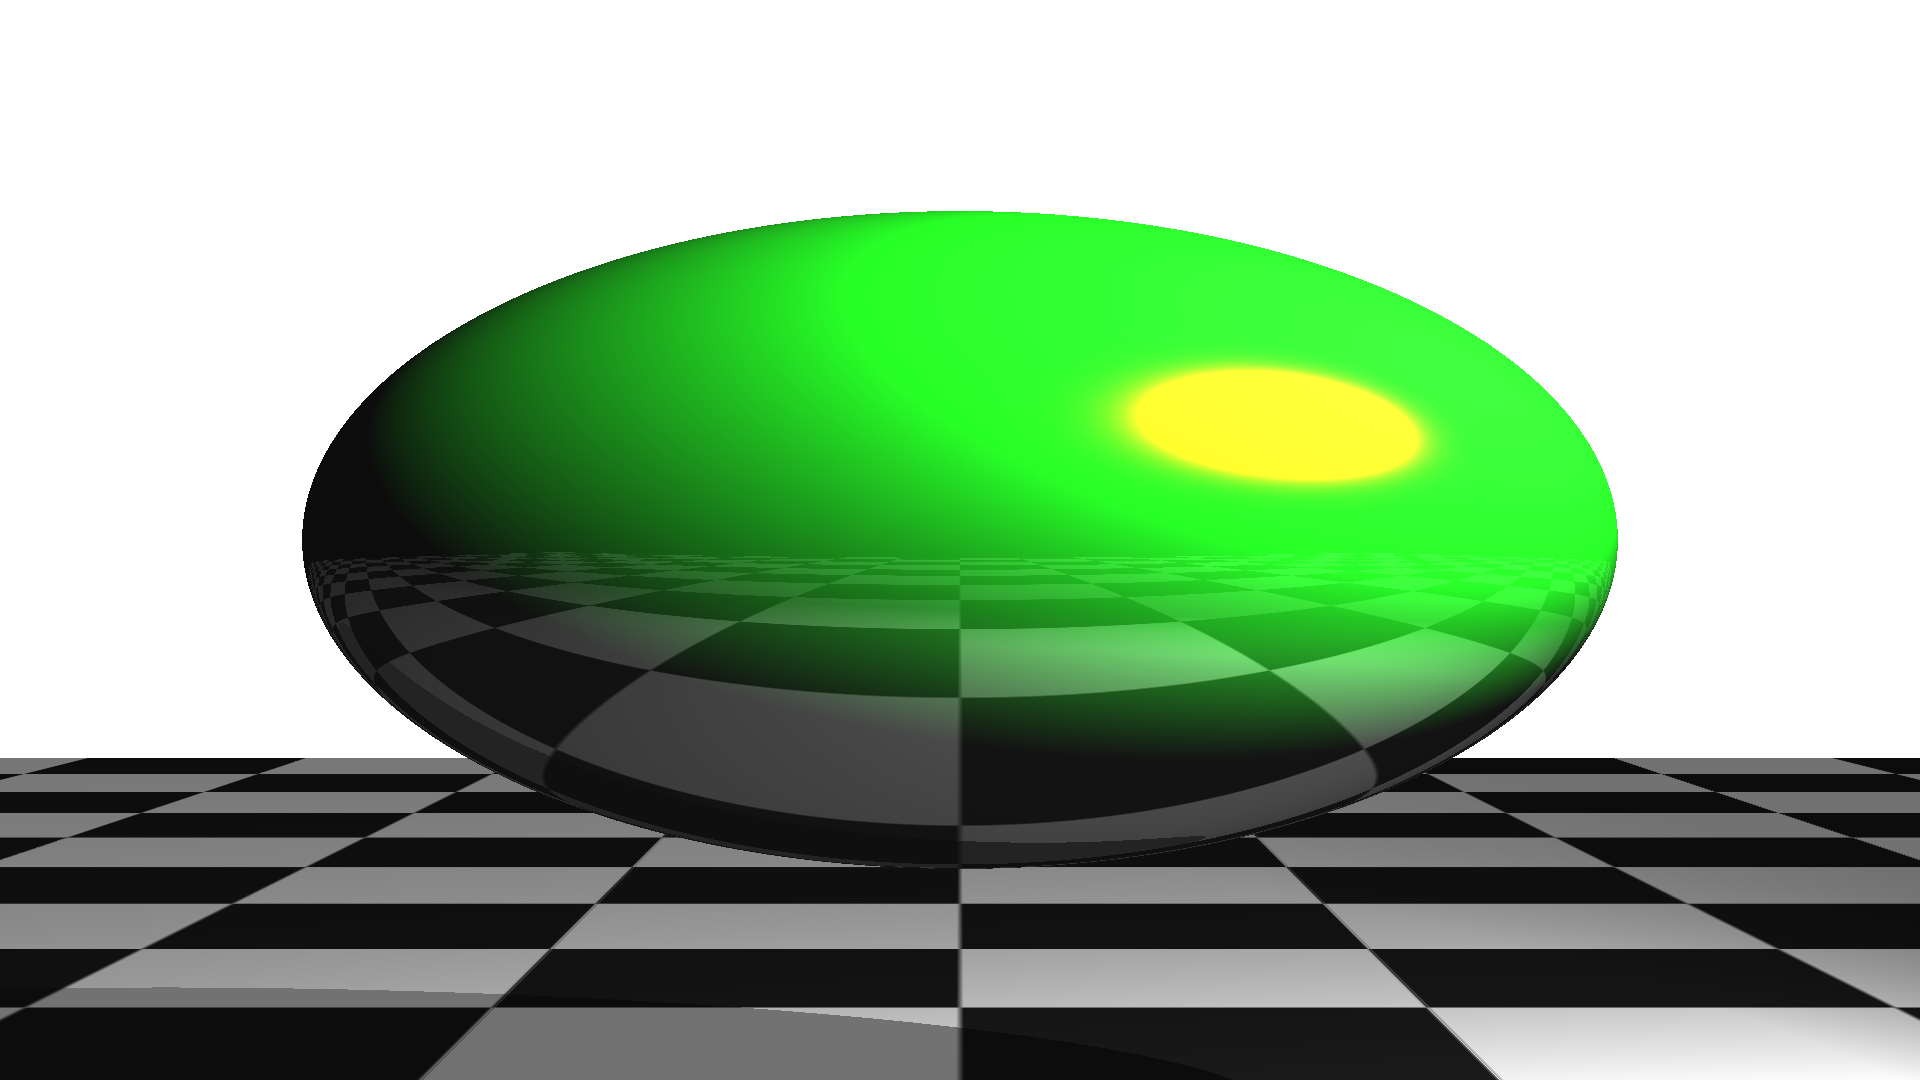
\includegraphics[width=0.3\textwidth]{chapters/ch3/img/reflection/specular_ks_02.png}}
\subfigure{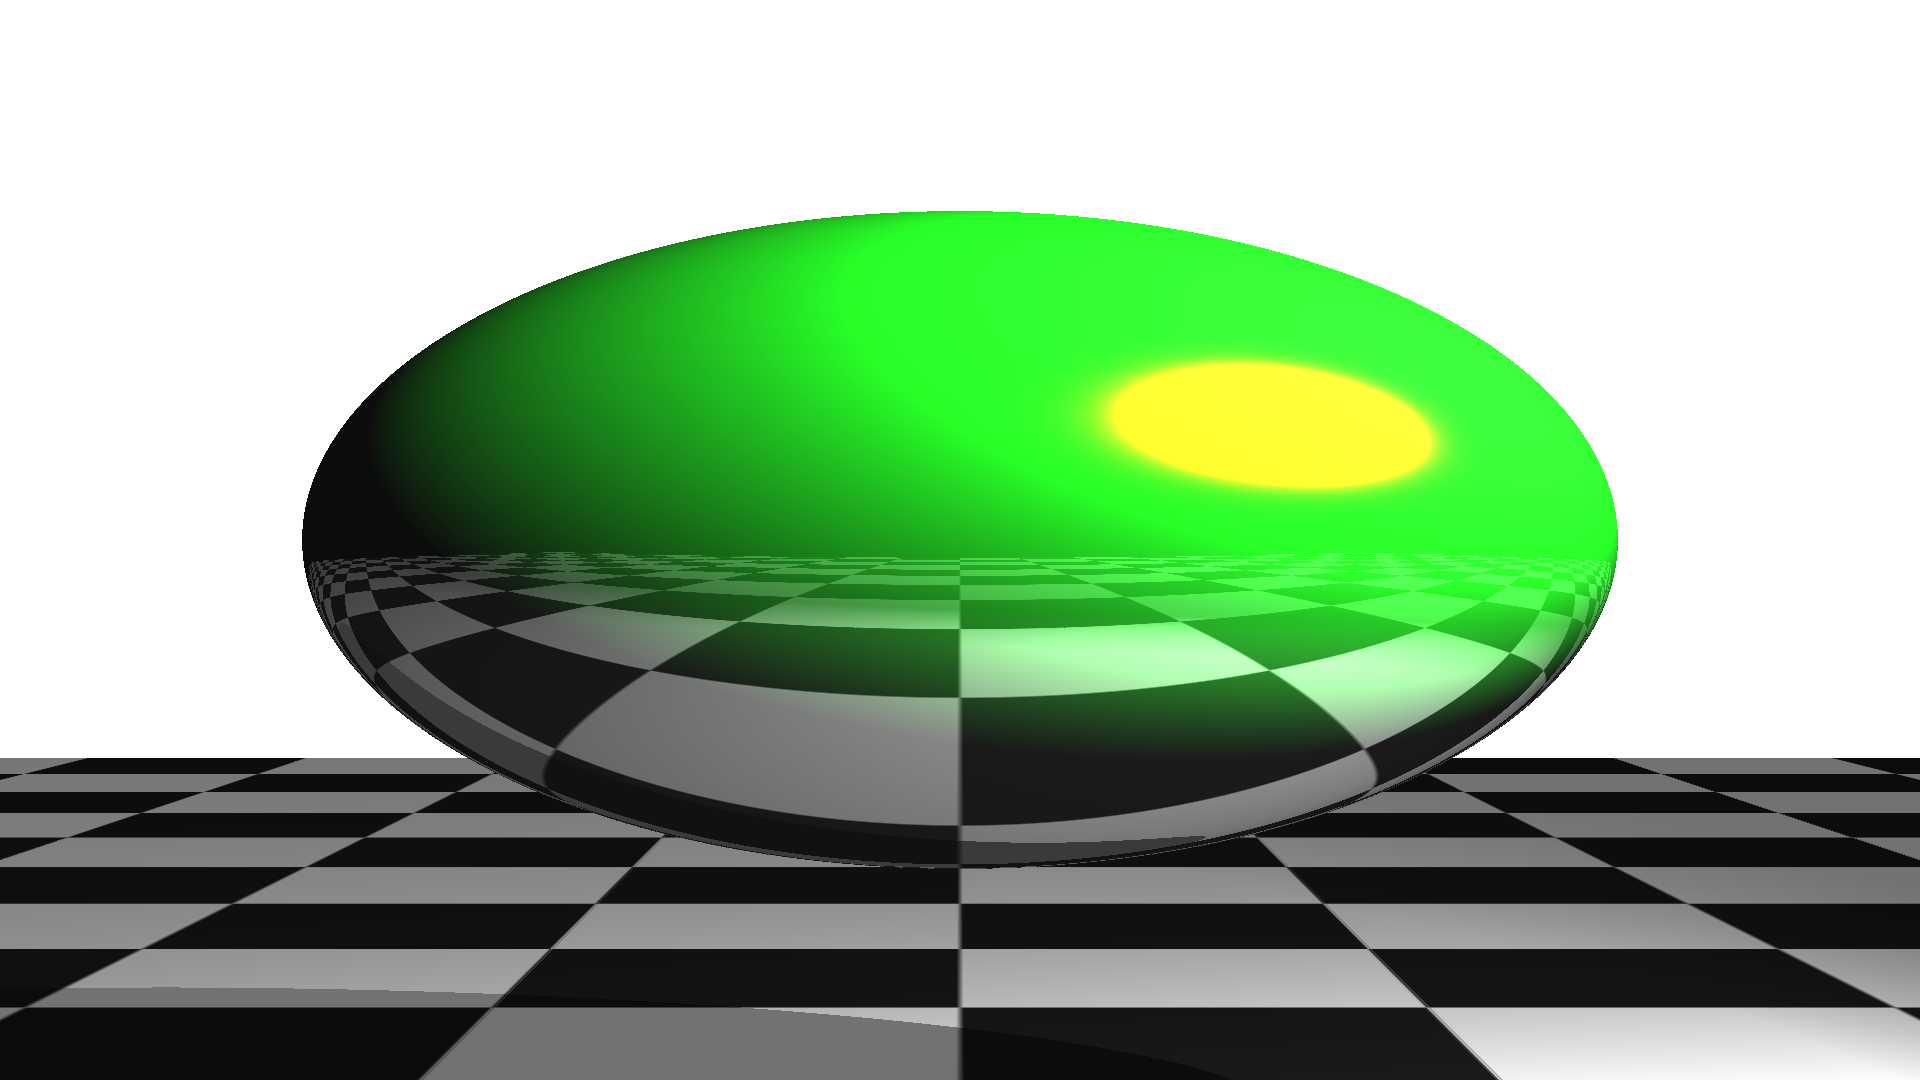
\includegraphics[width=0.3\textwidth]{chapters/ch3/img/reflection/specular_ks_04.png}}
\subfigure{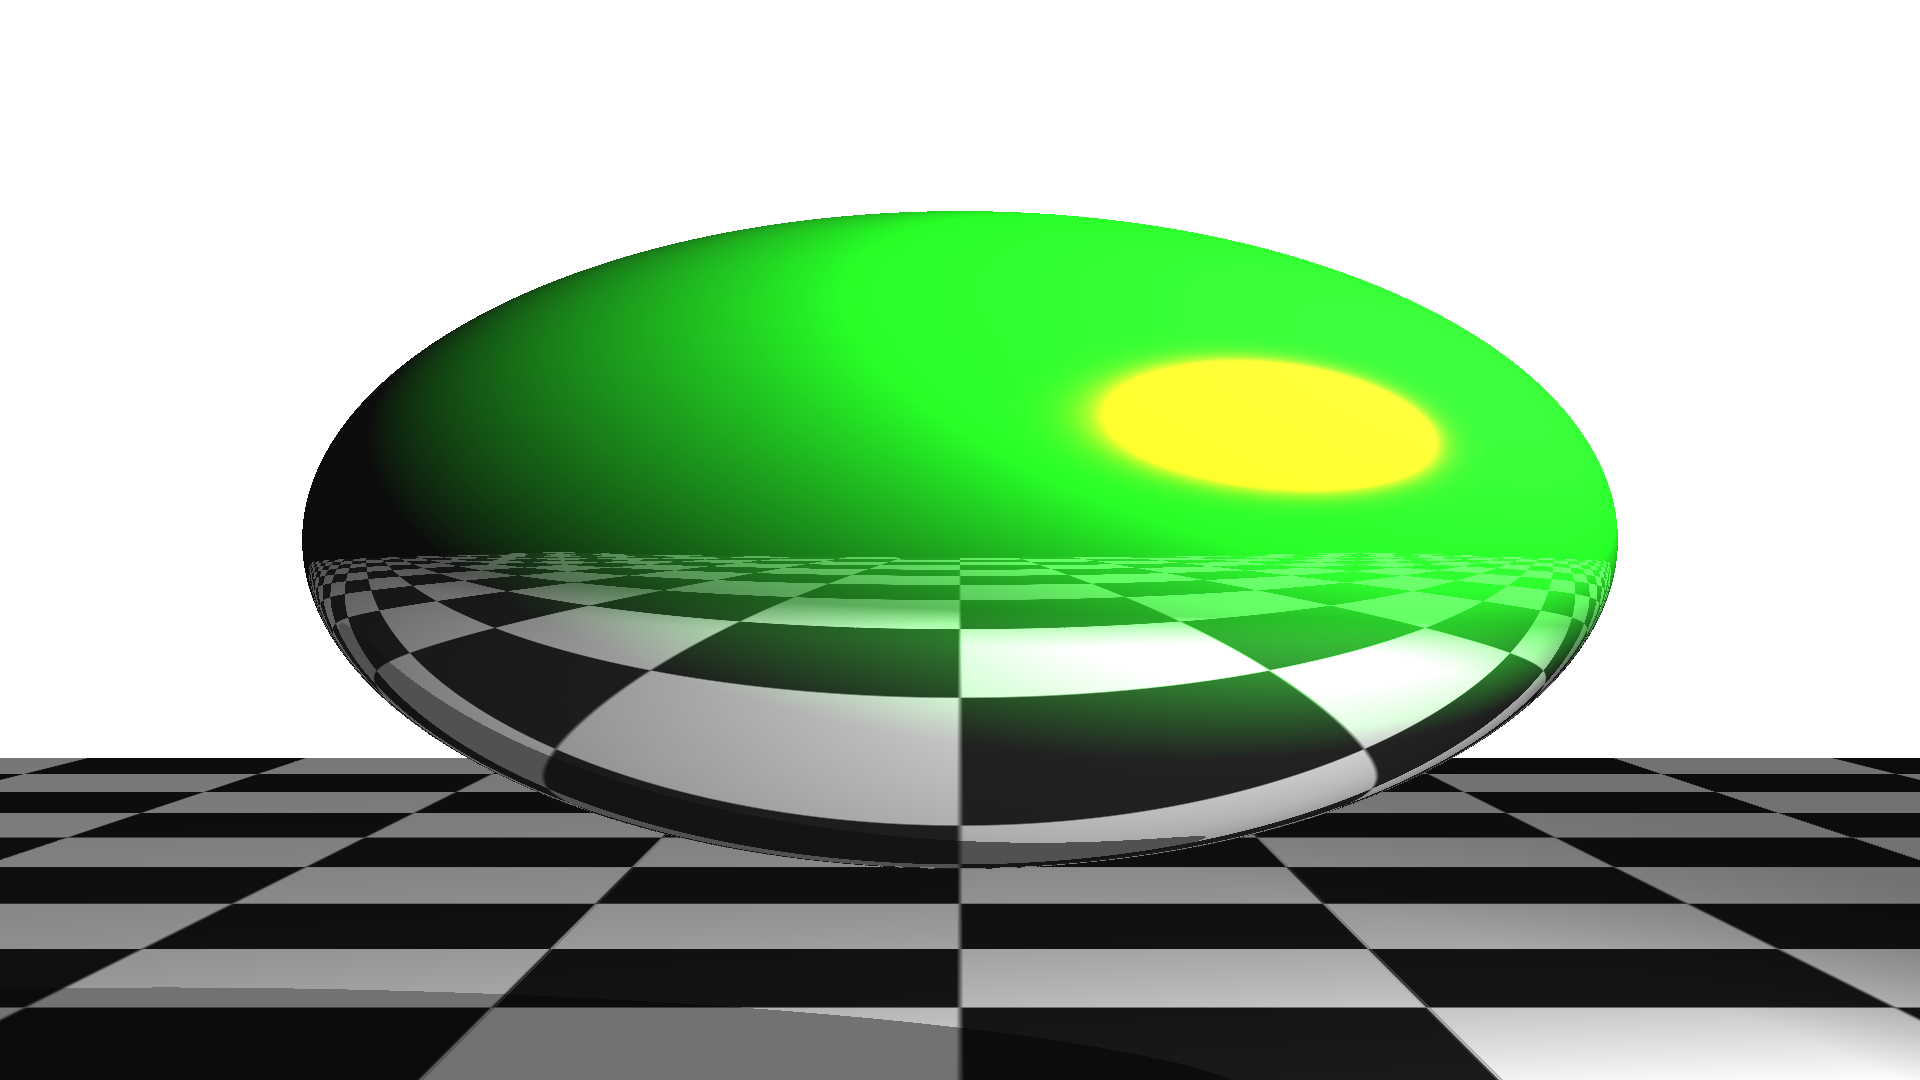
\includegraphics[width=0.3\textwidth]{chapters/ch3/img/reflection/specular_ks_06.png}}
\caption[Powierzchnie odbijające w sposób lustrzany]{Powierzchnie odbijające w sposób lustrzany w modelu Blinna-Phonga. Współczynnik odbicia $r_{l-1}$ jest stały, niezależny od kąta padania na płaszczyznę elipsoidy i równy współczynnikowi $k_s\in\lbrace 0,2; 0,4; 0,6 \rbrace$~($k_s$ rośnie od lewej do prawej)}
\label{ch3:img:reflection_types_specular}
\end{figure}

\begin{figure}[H]
\centering
\subfigure{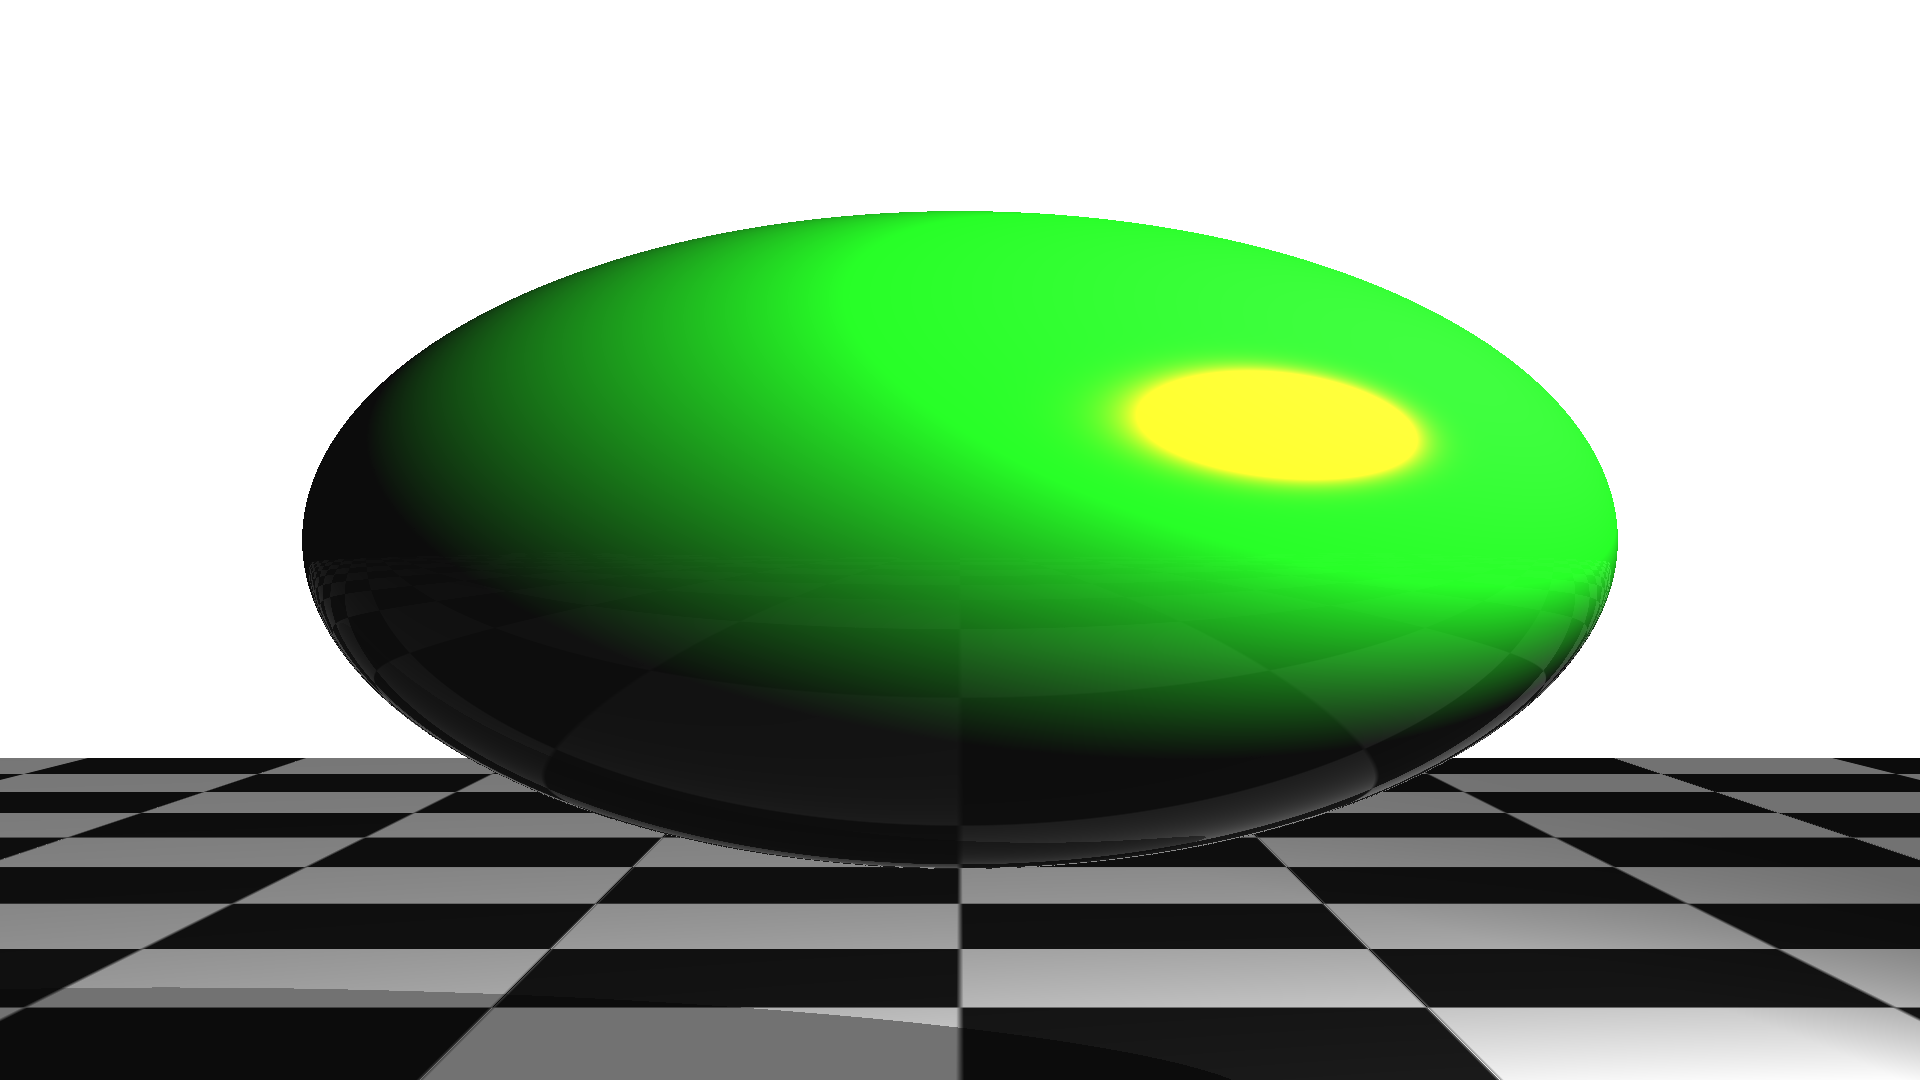
\includegraphics[width=0.3\textwidth]{chapters/ch3/img/reflection/fresnel_ks_02_exp_128_eta_133.png}}
\subfigure{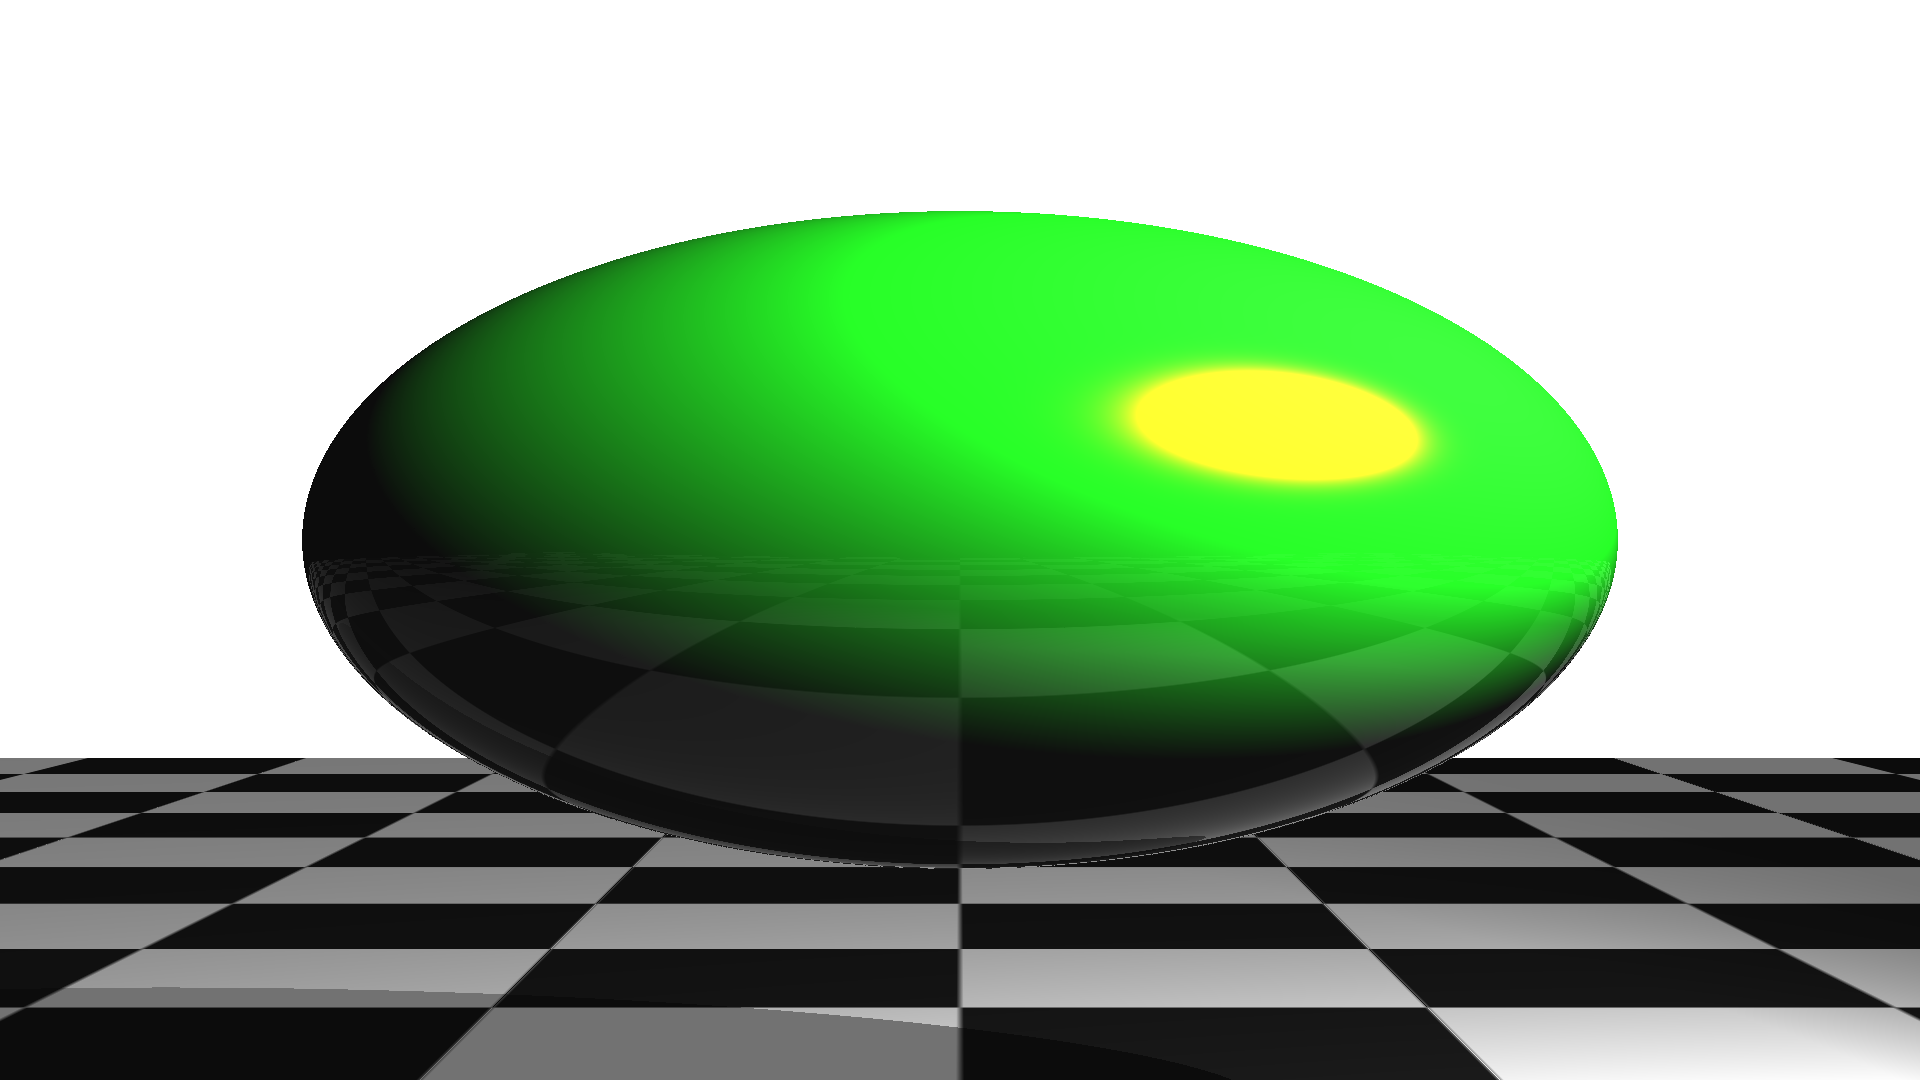
\includegraphics[width=0.3\textwidth]{chapters/ch3/img/reflection/fresnel_ks_02_exp_128_eta_166.png}}
\subfigure{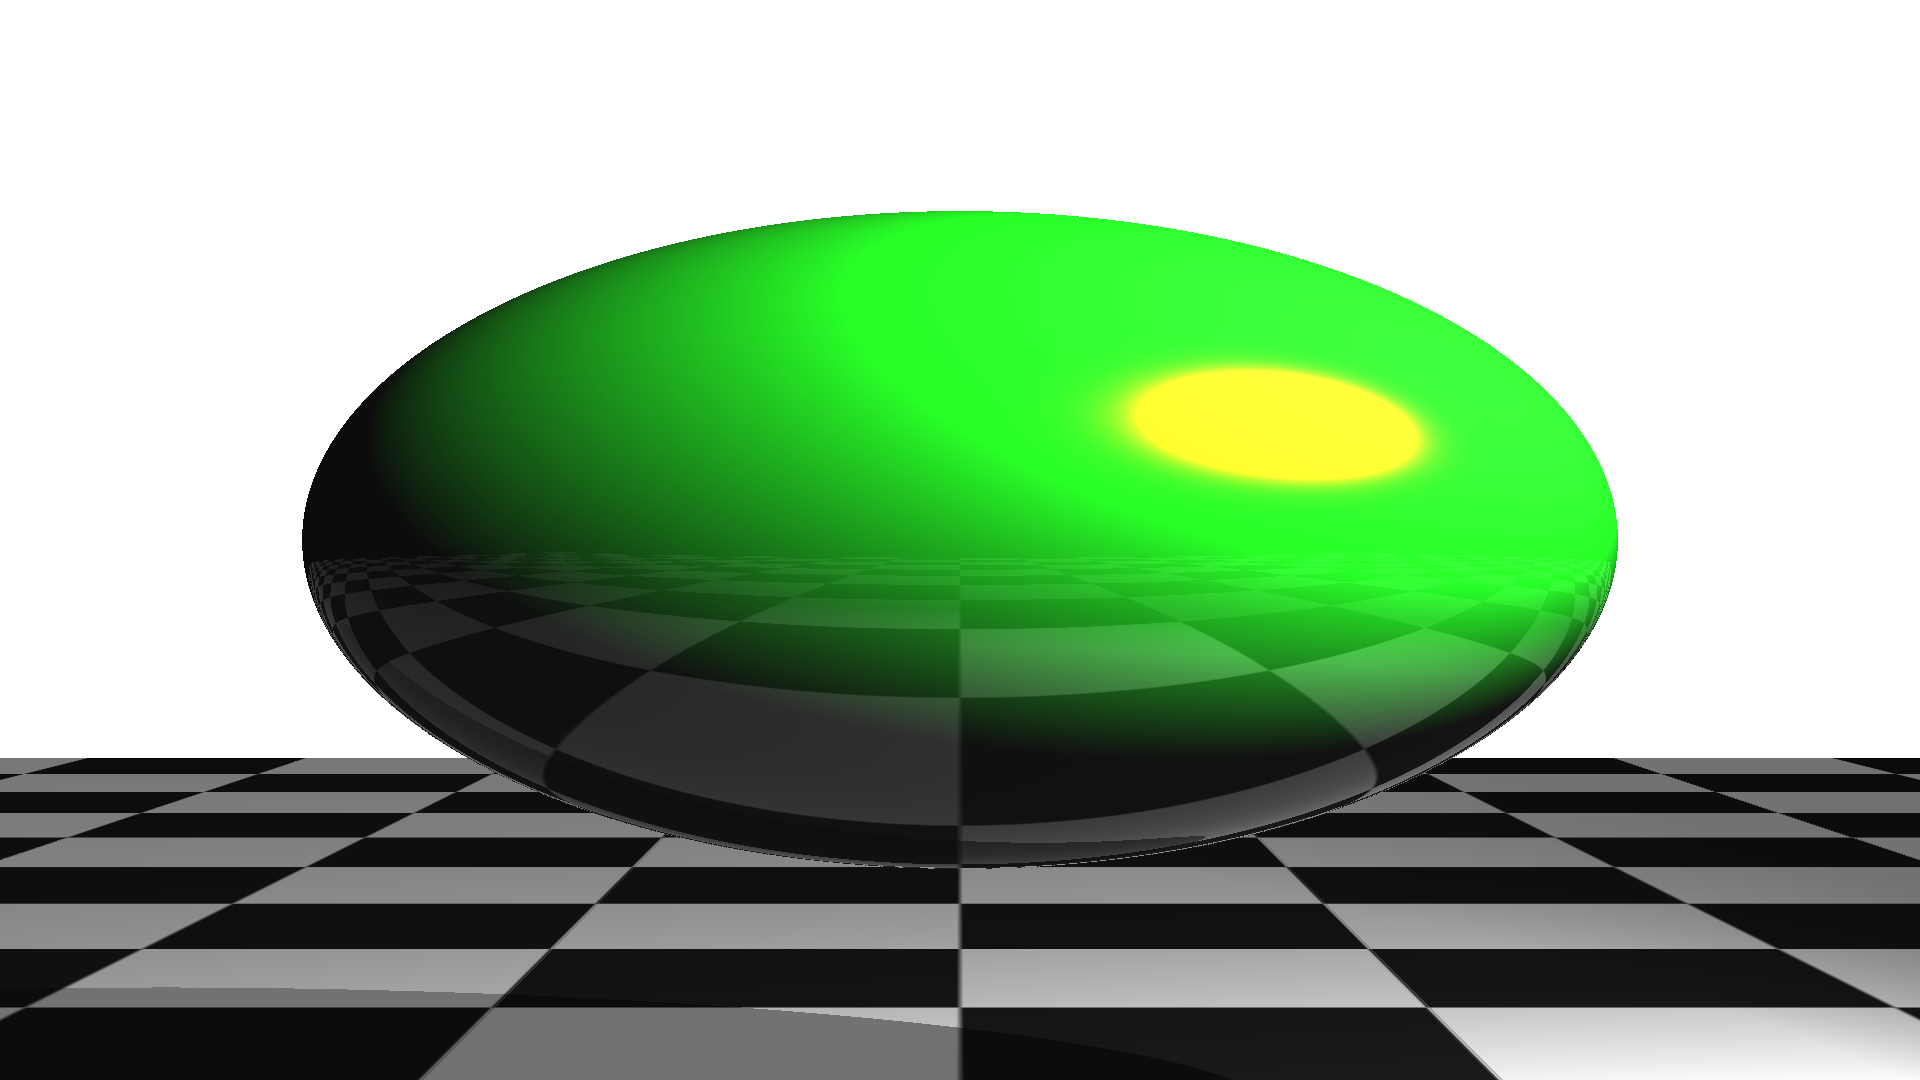
\includegraphics[width=0.3\textwidth]{chapters/ch3/img/reflection/fresnel_ks_02_exp_128_eta_200.png}}

\subfigure{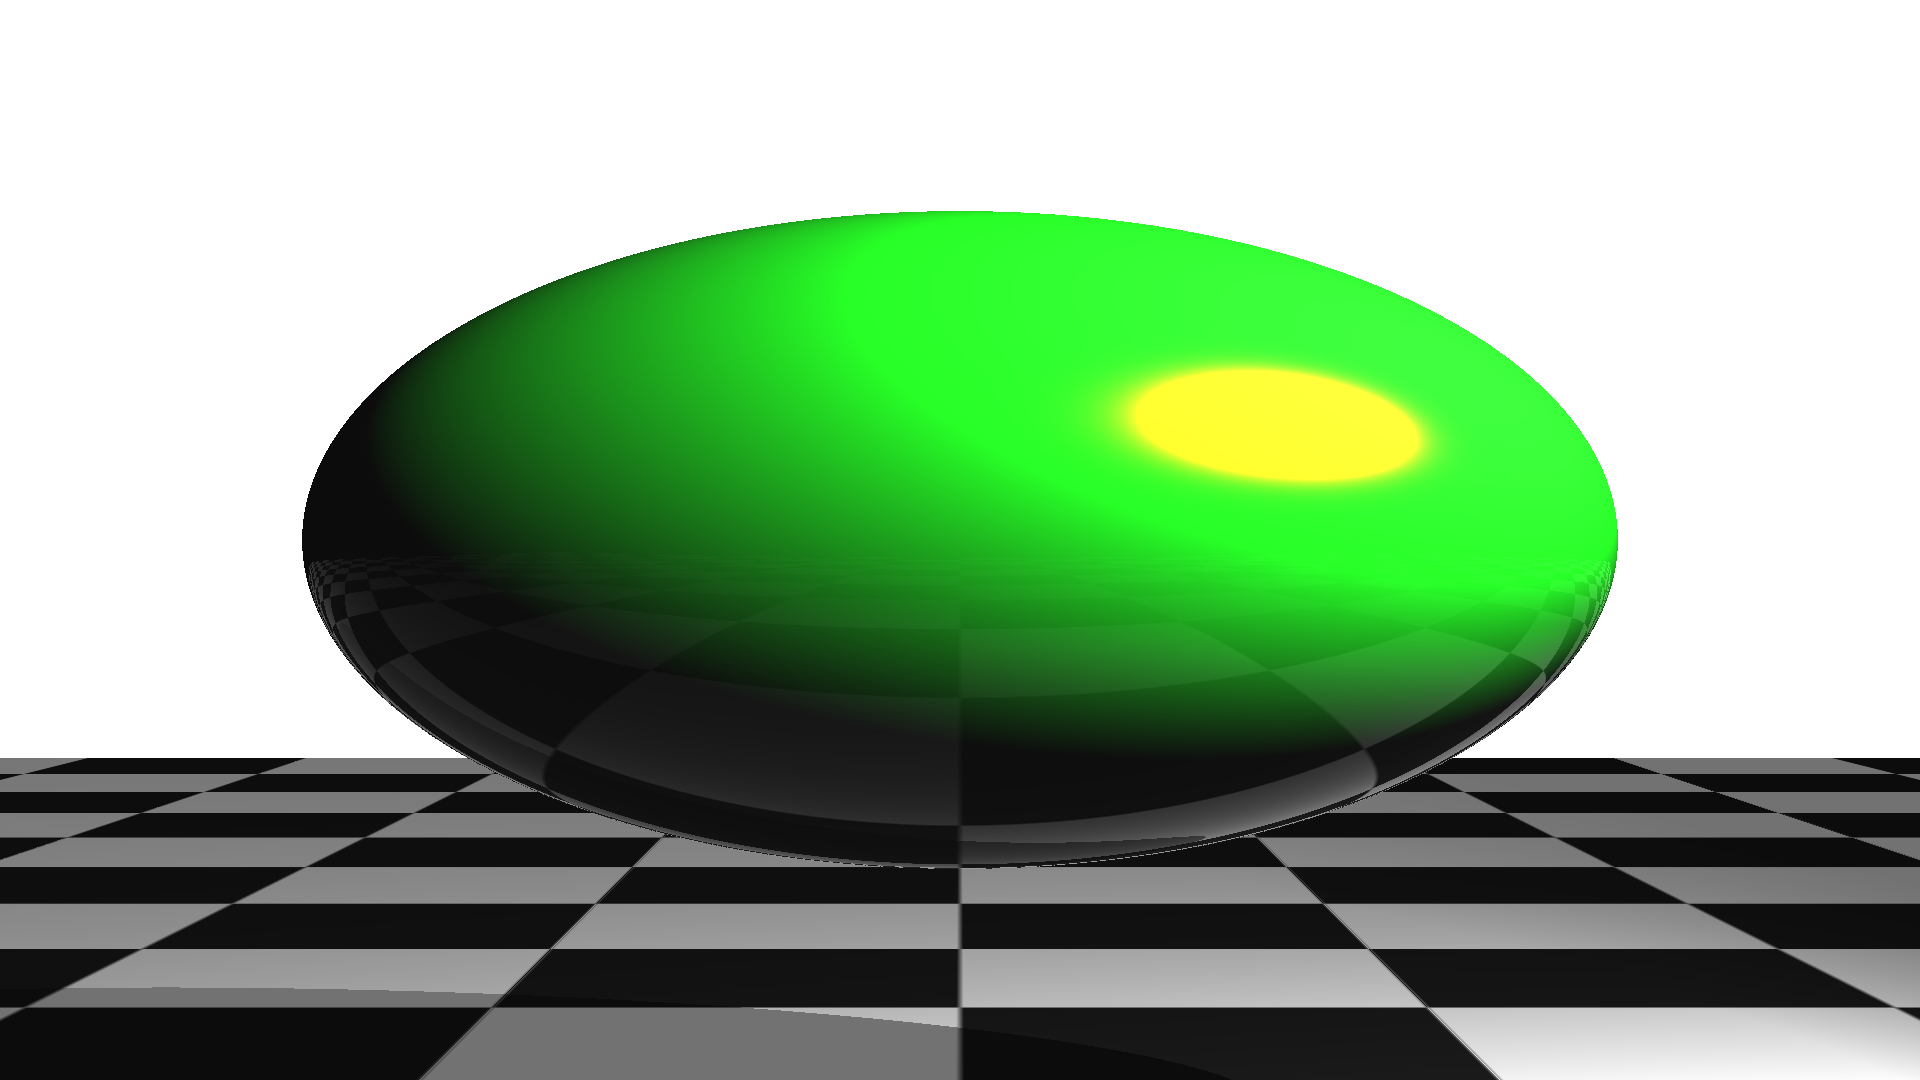
\includegraphics[width=0.3\textwidth]{chapters/ch3/img/reflection/fresnel_ks_02_exp_128_eta_133_k_02.png}}
\subfigure{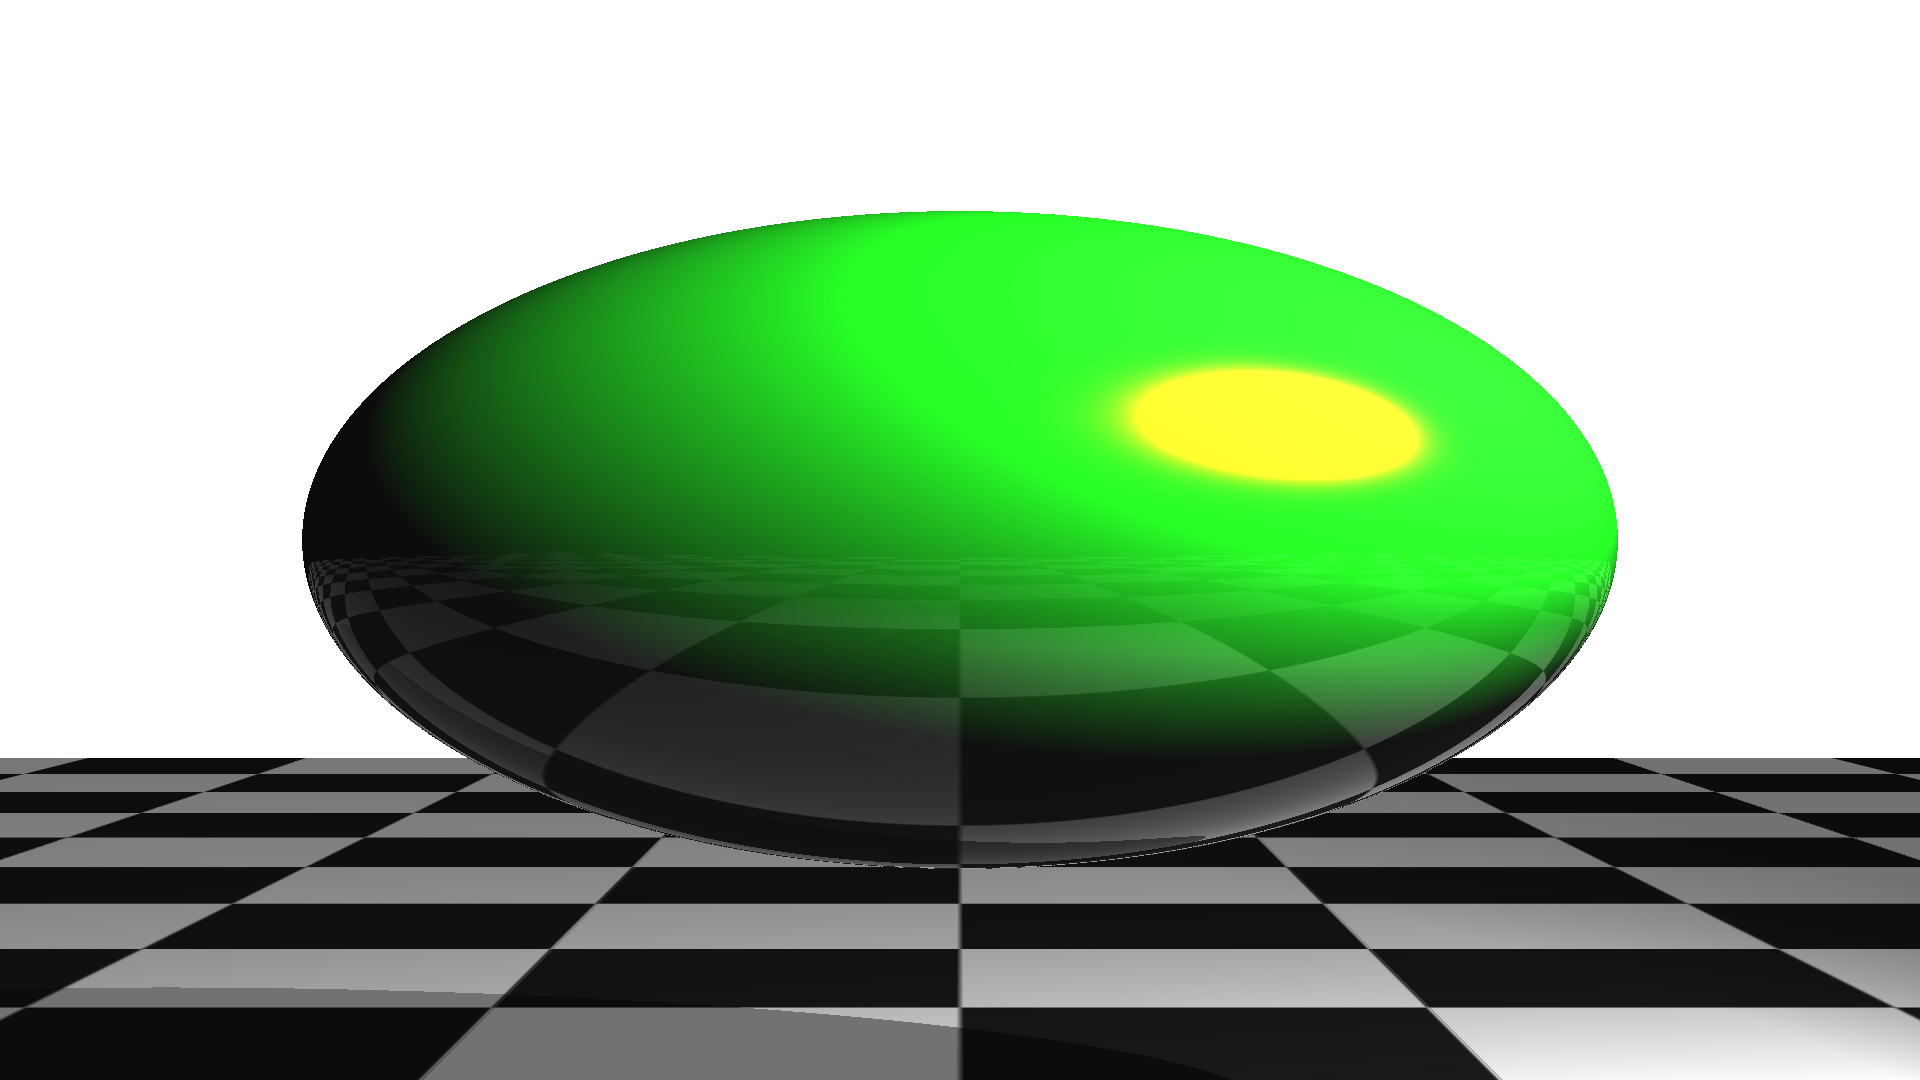
\includegraphics[width=0.3\textwidth]{chapters/ch3/img/reflection/fresnel_ks_02_exp_128_eta_133_k_06.png}}
\subfigure{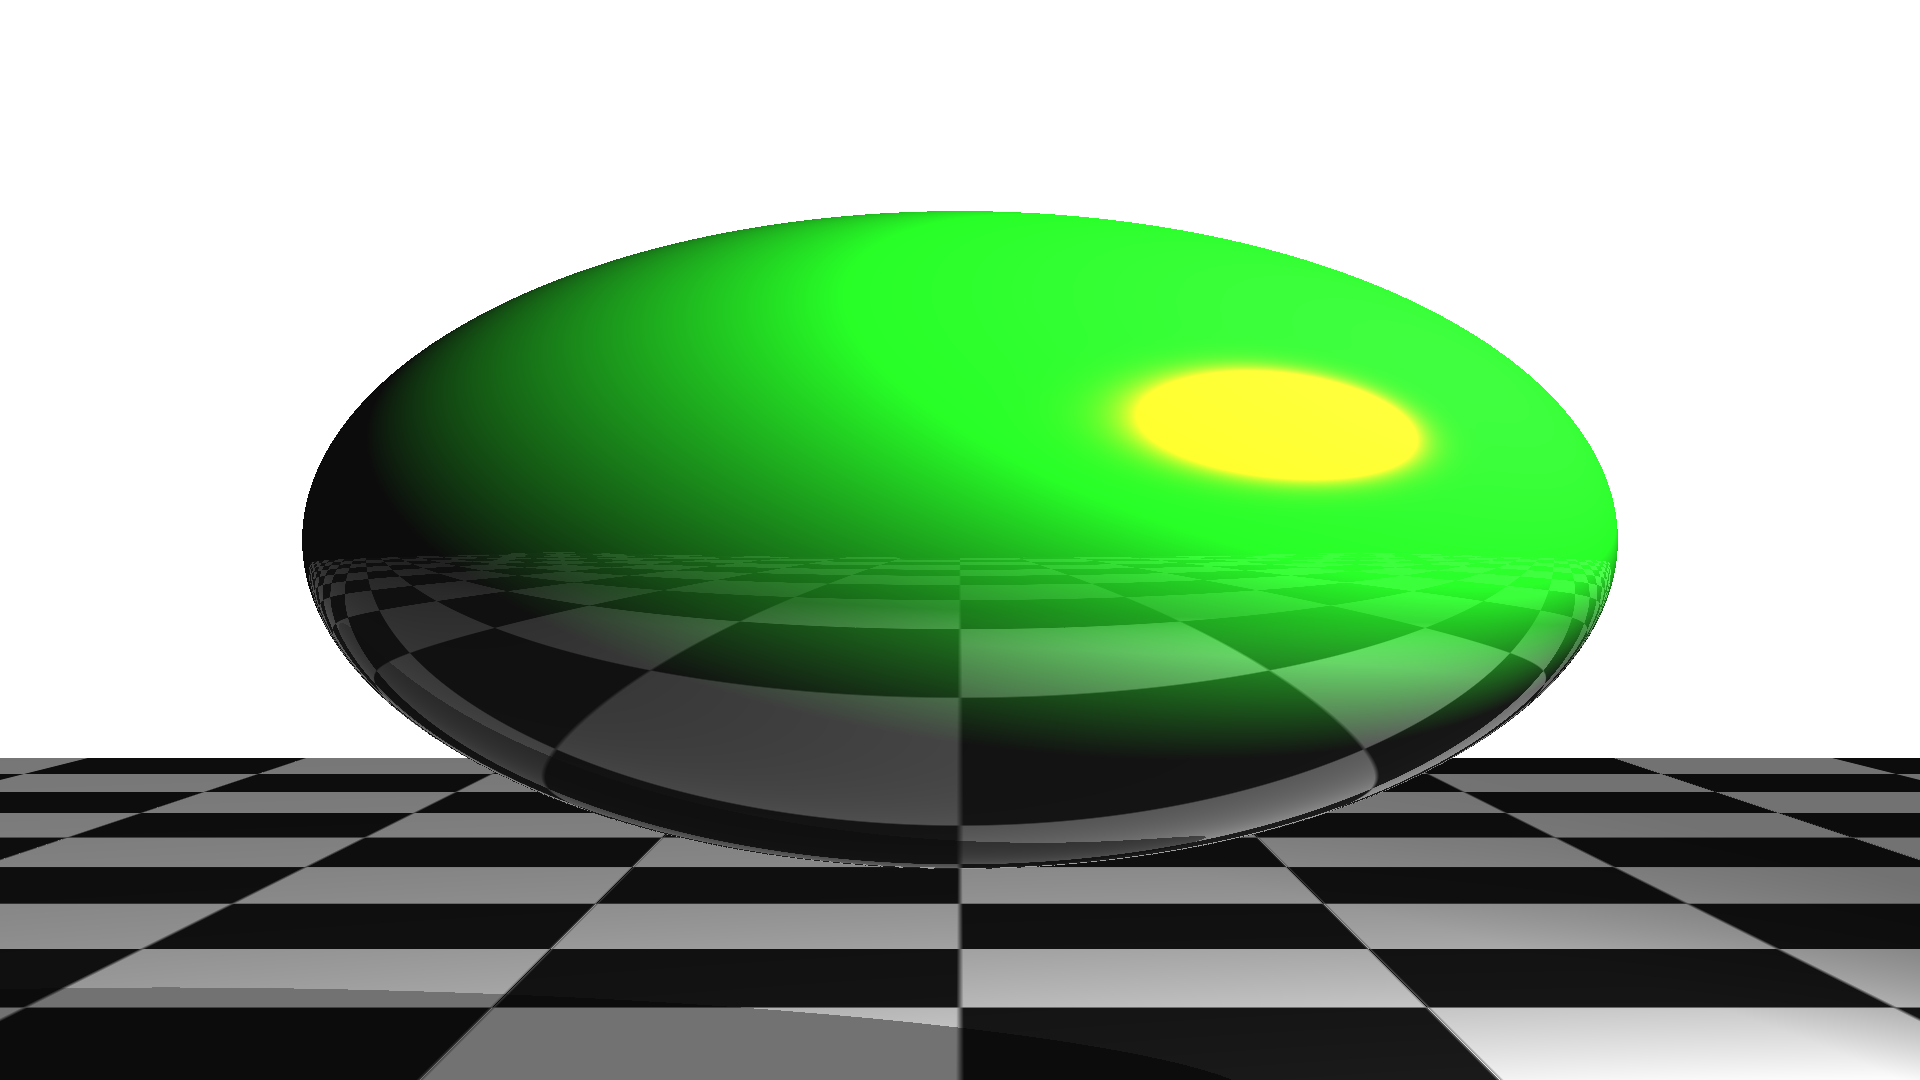
\includegraphics[width=0.3\textwidth]{chapters/ch3/img/reflection/fresnel_ks_02_exp_128_eta_133_k_10.png}}
\caption[Powierzchnie odbijające zgodnie ze wzorami Fresnela]{Powierzchnie odbijające zgodnie ze wzorami Fresnela w modelu Blinna-Phonga. Obrazy w górnym wierszu odpowiadają dielektrykom~($k=0$) o współczynniku załamania (od lewej do prawej) $\eta\in\lbrace 1,33; 1,66; 2,00 \rbrace$. Dla najmniejszego ze współczynników załamania $\eta=1,33$ odbicia są słabo zauważalne, jednak $r_{l-1}$ rośnie bardzo szybko, gdy promień padający staje się styczny do powierzchni. W dolnym wierszu przedstawione zostały przewodniki o~$k\in\lbrace 0,2; 0,6; 1,0 \rbrace$ i $\eta = 1,33$, których powierzchnie są znacznie bardziej odbijające niż w~przypadku dielektryka o tym samym $\eta$}
\label{ch3:img:reflection_types_fresnel}
\end{figure}

Zastosowanie modelu Torrance'a-Sparrowa na rysunku~\ref{ch3:img:reflection_types_ts} zamiast modelu Blinna-Phonga z odbiciem Fresnela~(rysunek~\ref{ch3:img:reflection_types_fresnel}) wprowadza dwie główne zmiany w obrazie:
\begin{enumerate}
\item Siła rozbłysku w prawej górnej części elipsoidy jest mniejsza i należy stosować większy współczynnik skupienia $e$.
\item Współczynnik odbicia, ze względu na sposób jego określenia w modelu Torrance'a-Sparrowa między wektorem połówkowym $\vec{\omega_h}$ a $\vec{\omega_o}$, nie rośnie tak szybko wraz ze~wzrostem kąta padania.   
\end{enumerate}

\begin{figure}[H]
\centering

\subfigure{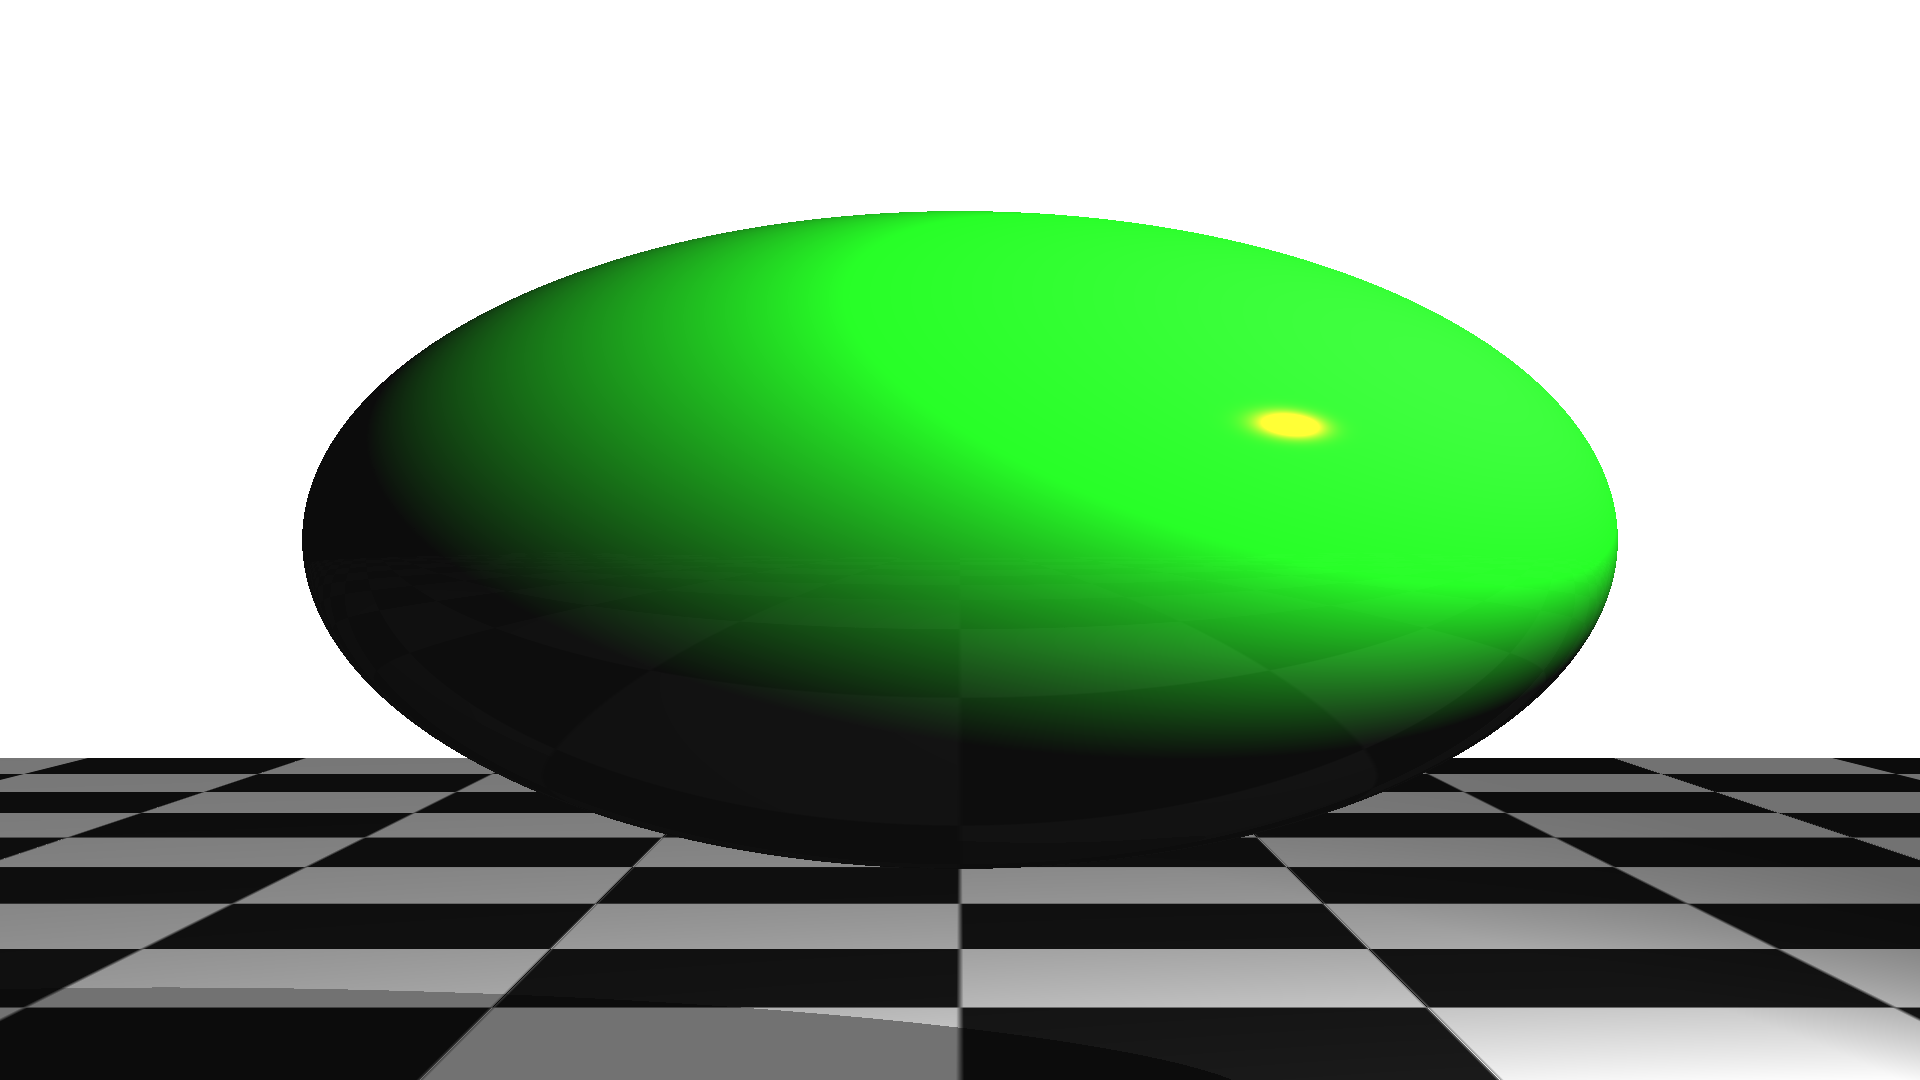
\includegraphics[width=0.3\textwidth]{chapters/ch3/img/reflection/ts_ks_06_exp_1024_eta_133.png}}
\subfigure{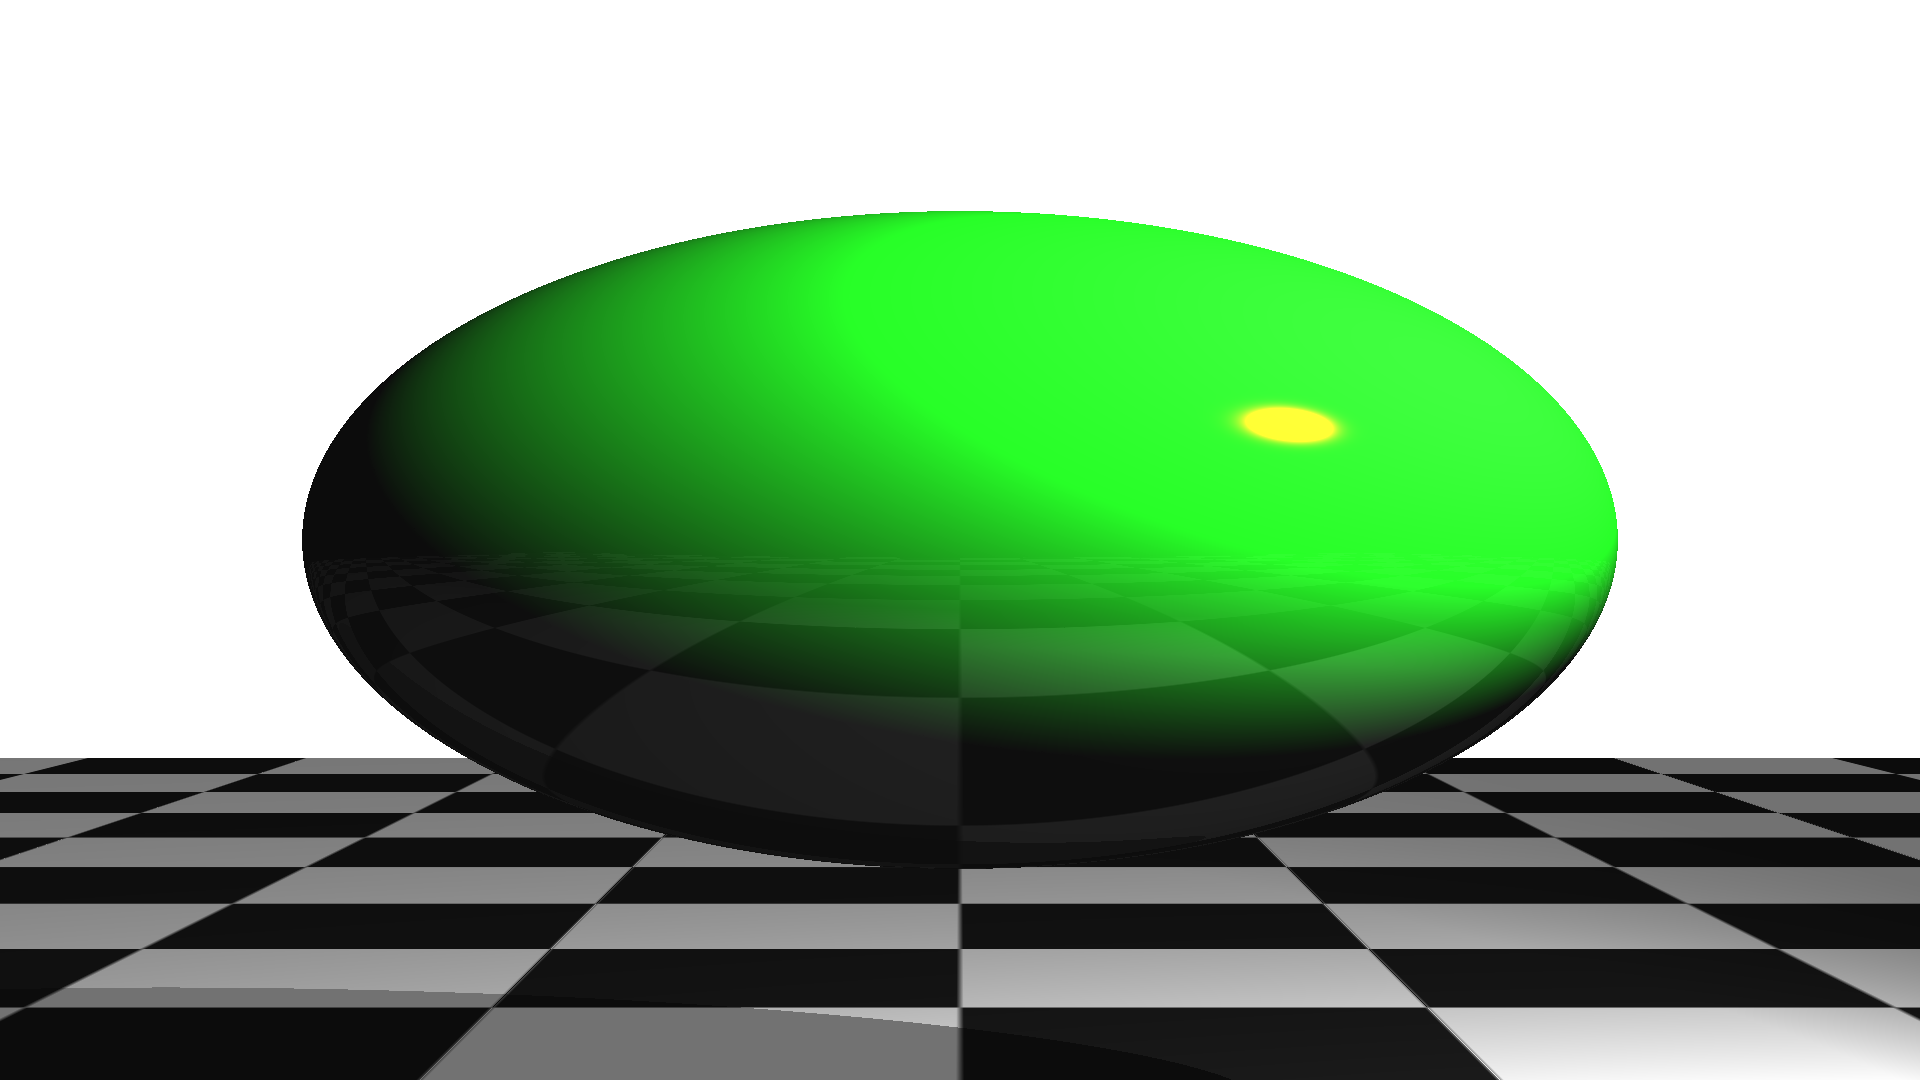
\includegraphics[width=0.3\textwidth]{chapters/ch3/img/reflection/ts_ks_06_exp_1024_eta_166.png}}
\subfigure{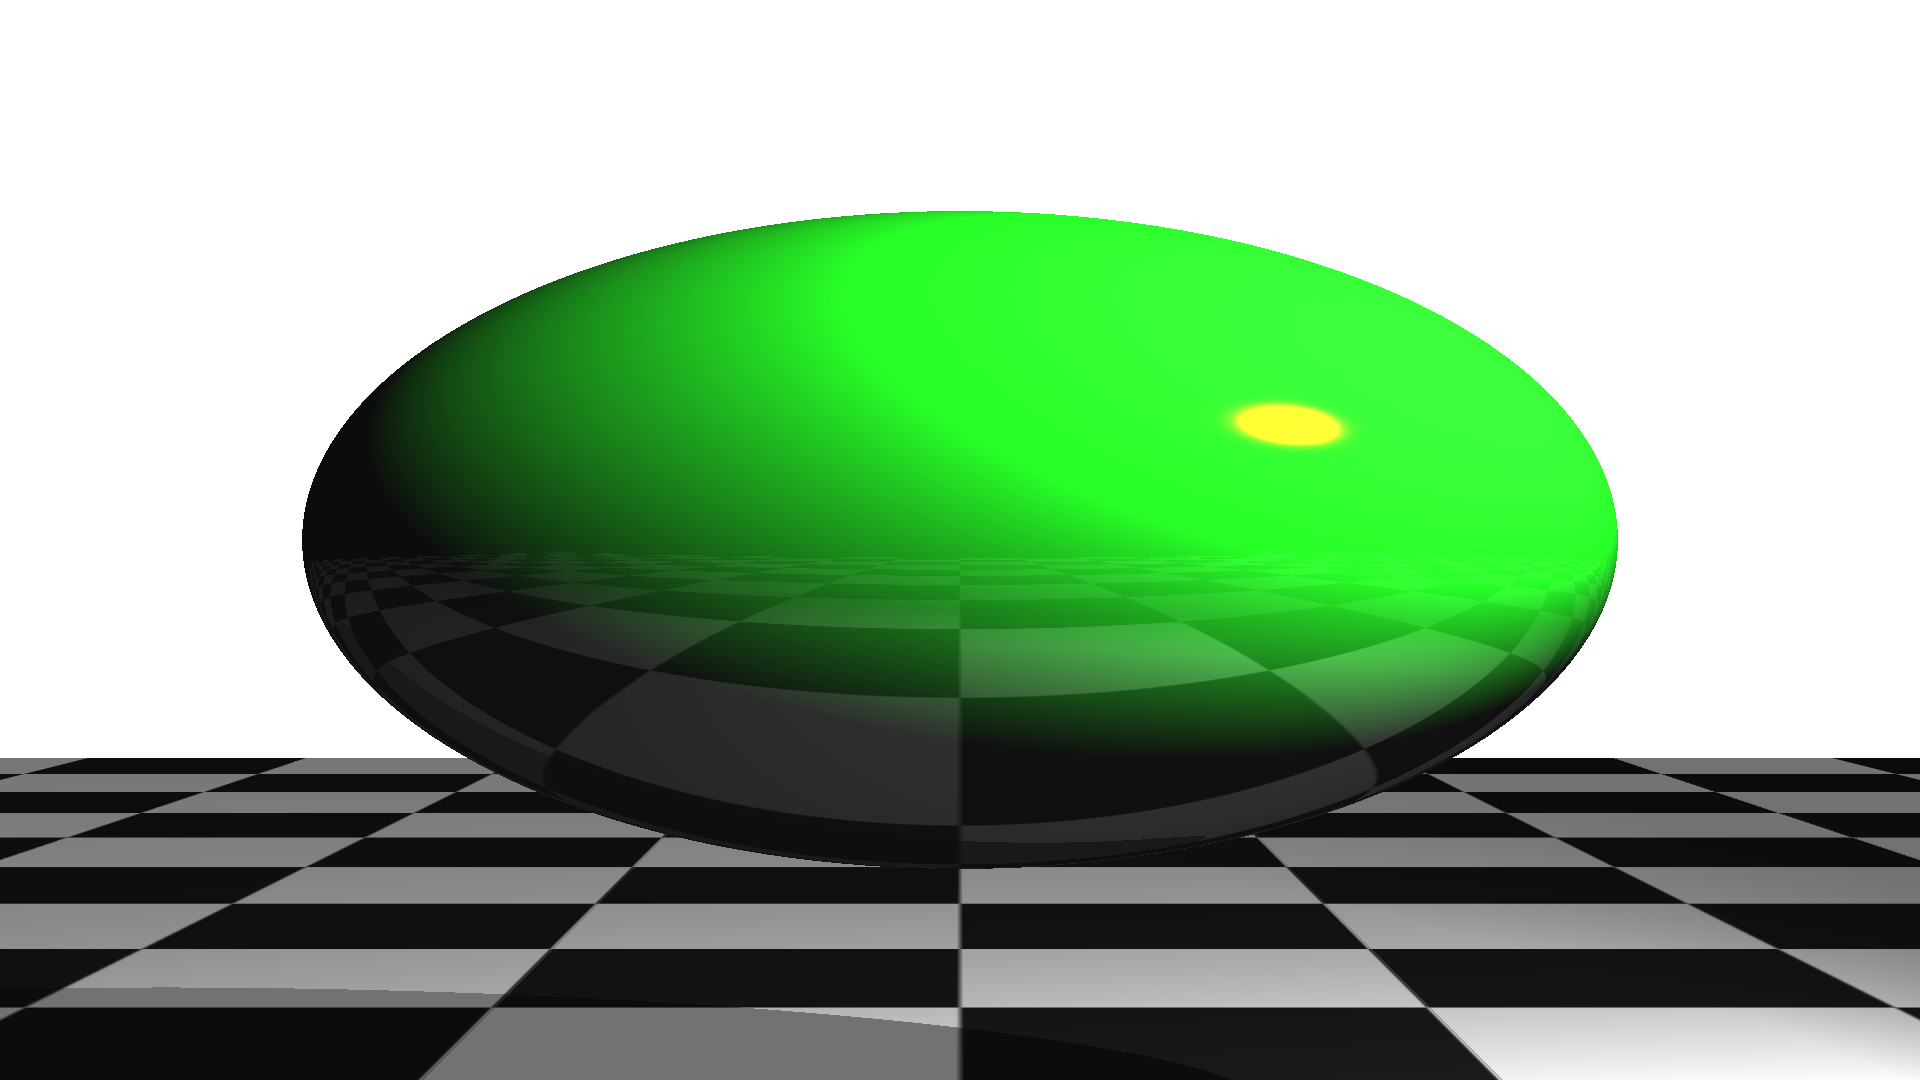
\includegraphics[width=0.3\textwidth]{chapters/ch3/img/reflection/ts_ks_06_exp_1024_eta_200.png}}

\subfigure{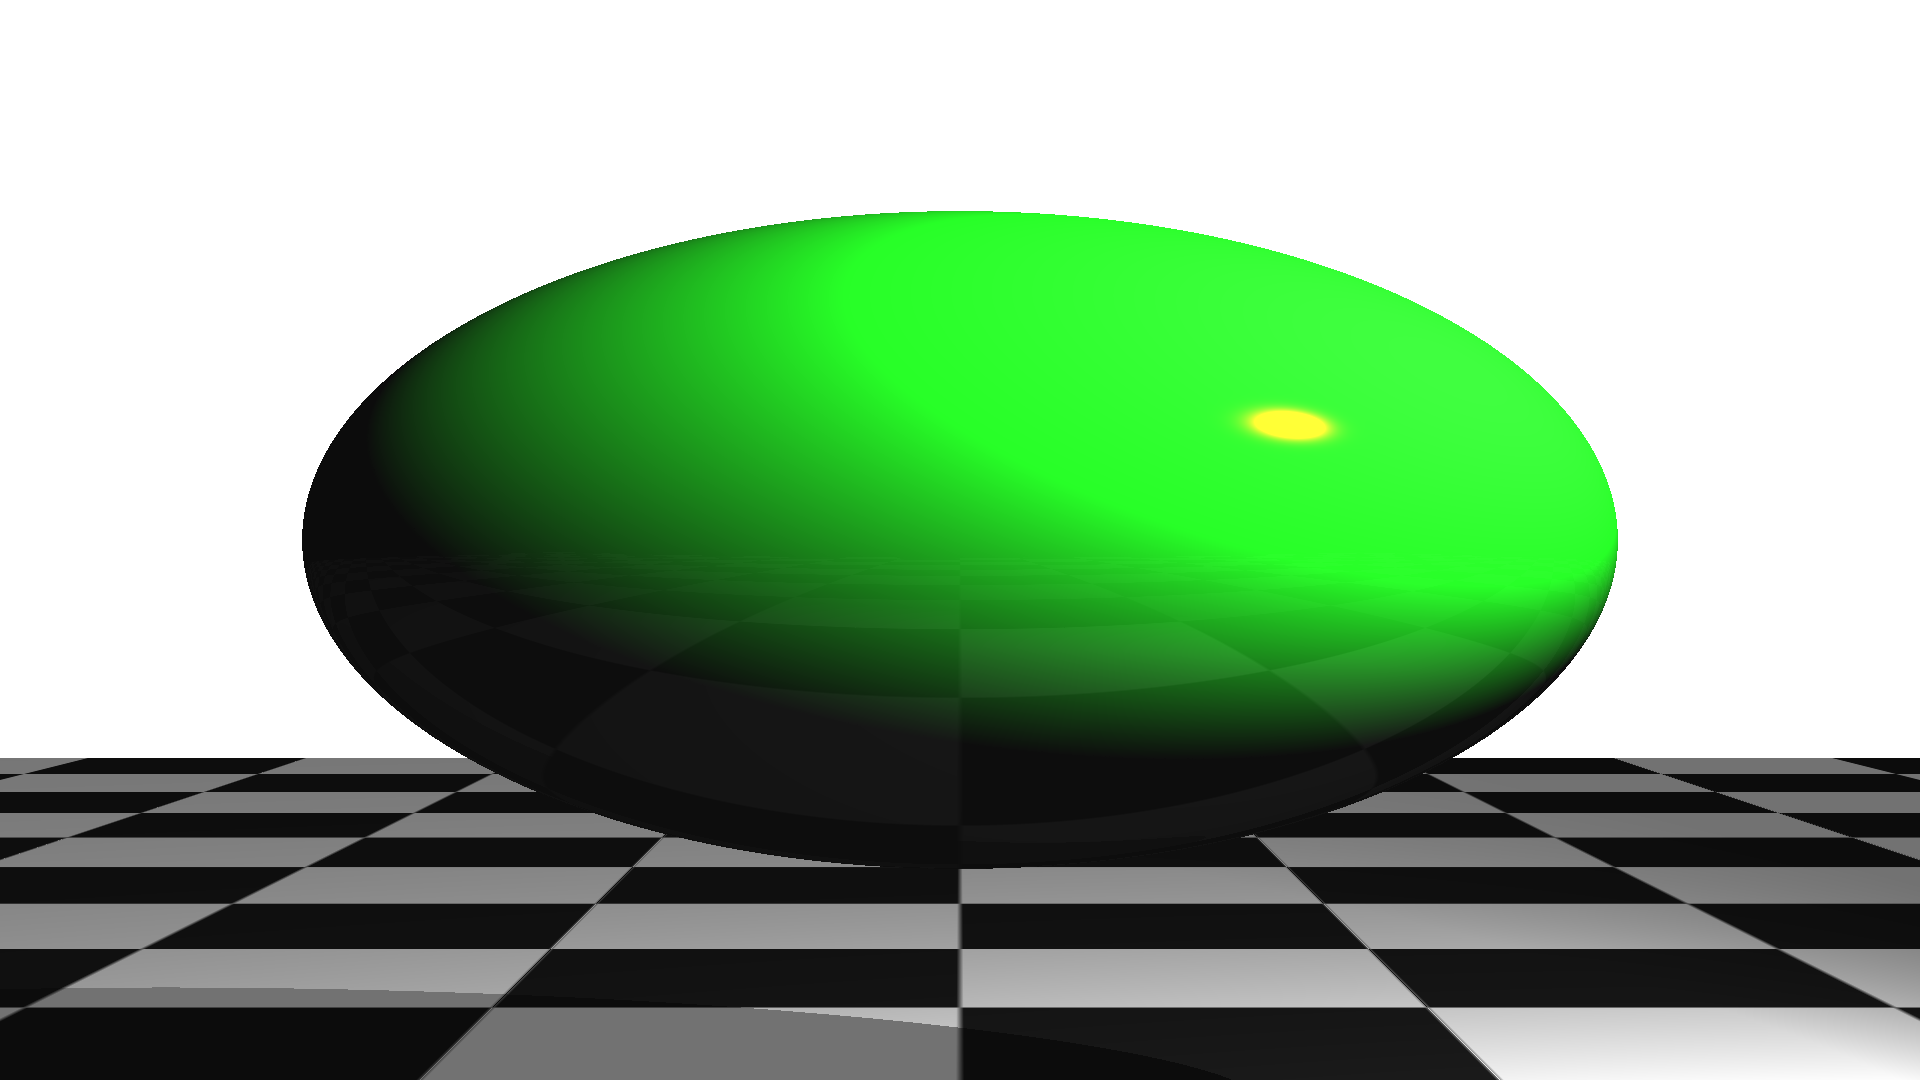
\includegraphics[width=0.3\textwidth]{chapters/ch3/img/reflection/ts_ks_06_exp_1024_eta_133_k_02.png}}
\subfigure{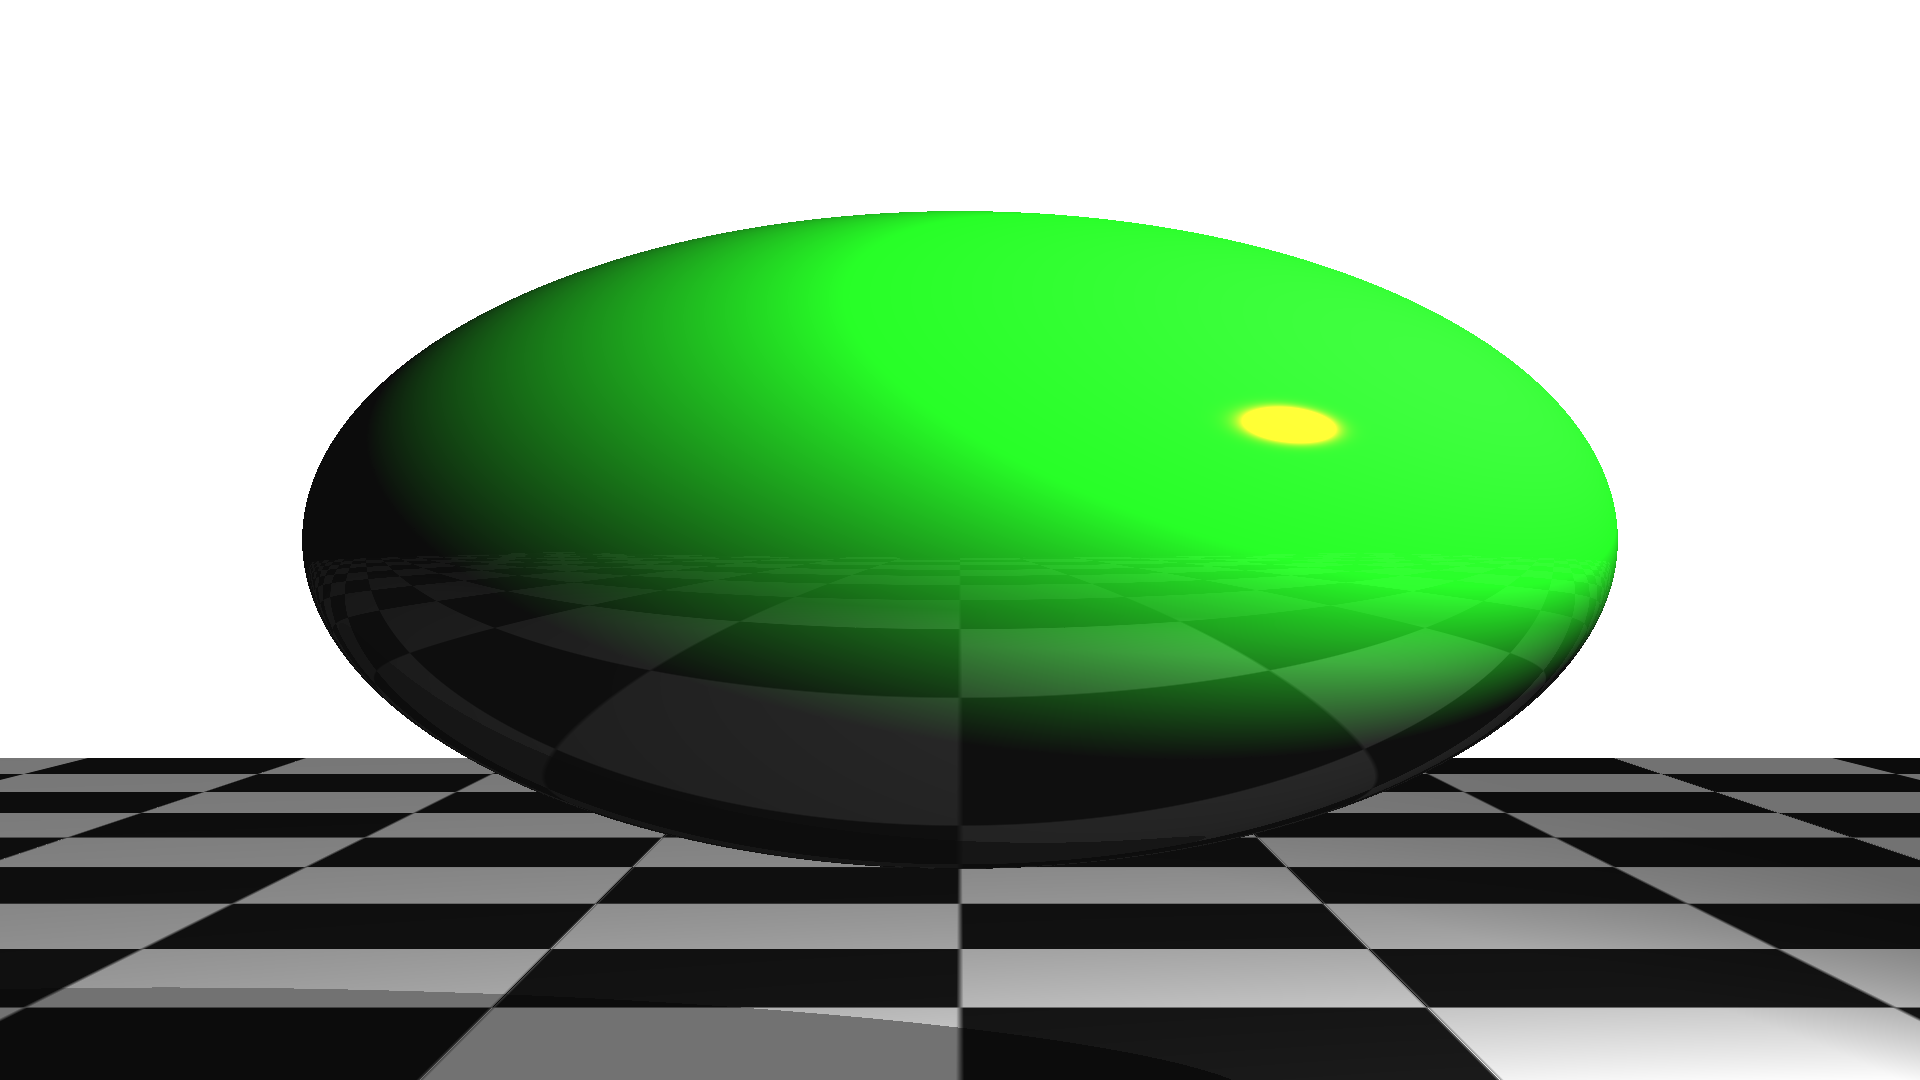
\includegraphics[width=0.3\textwidth]{chapters/ch3/img/reflection/ts_ks_06_exp_1024_eta_133_k_06.png}}
\subfigure{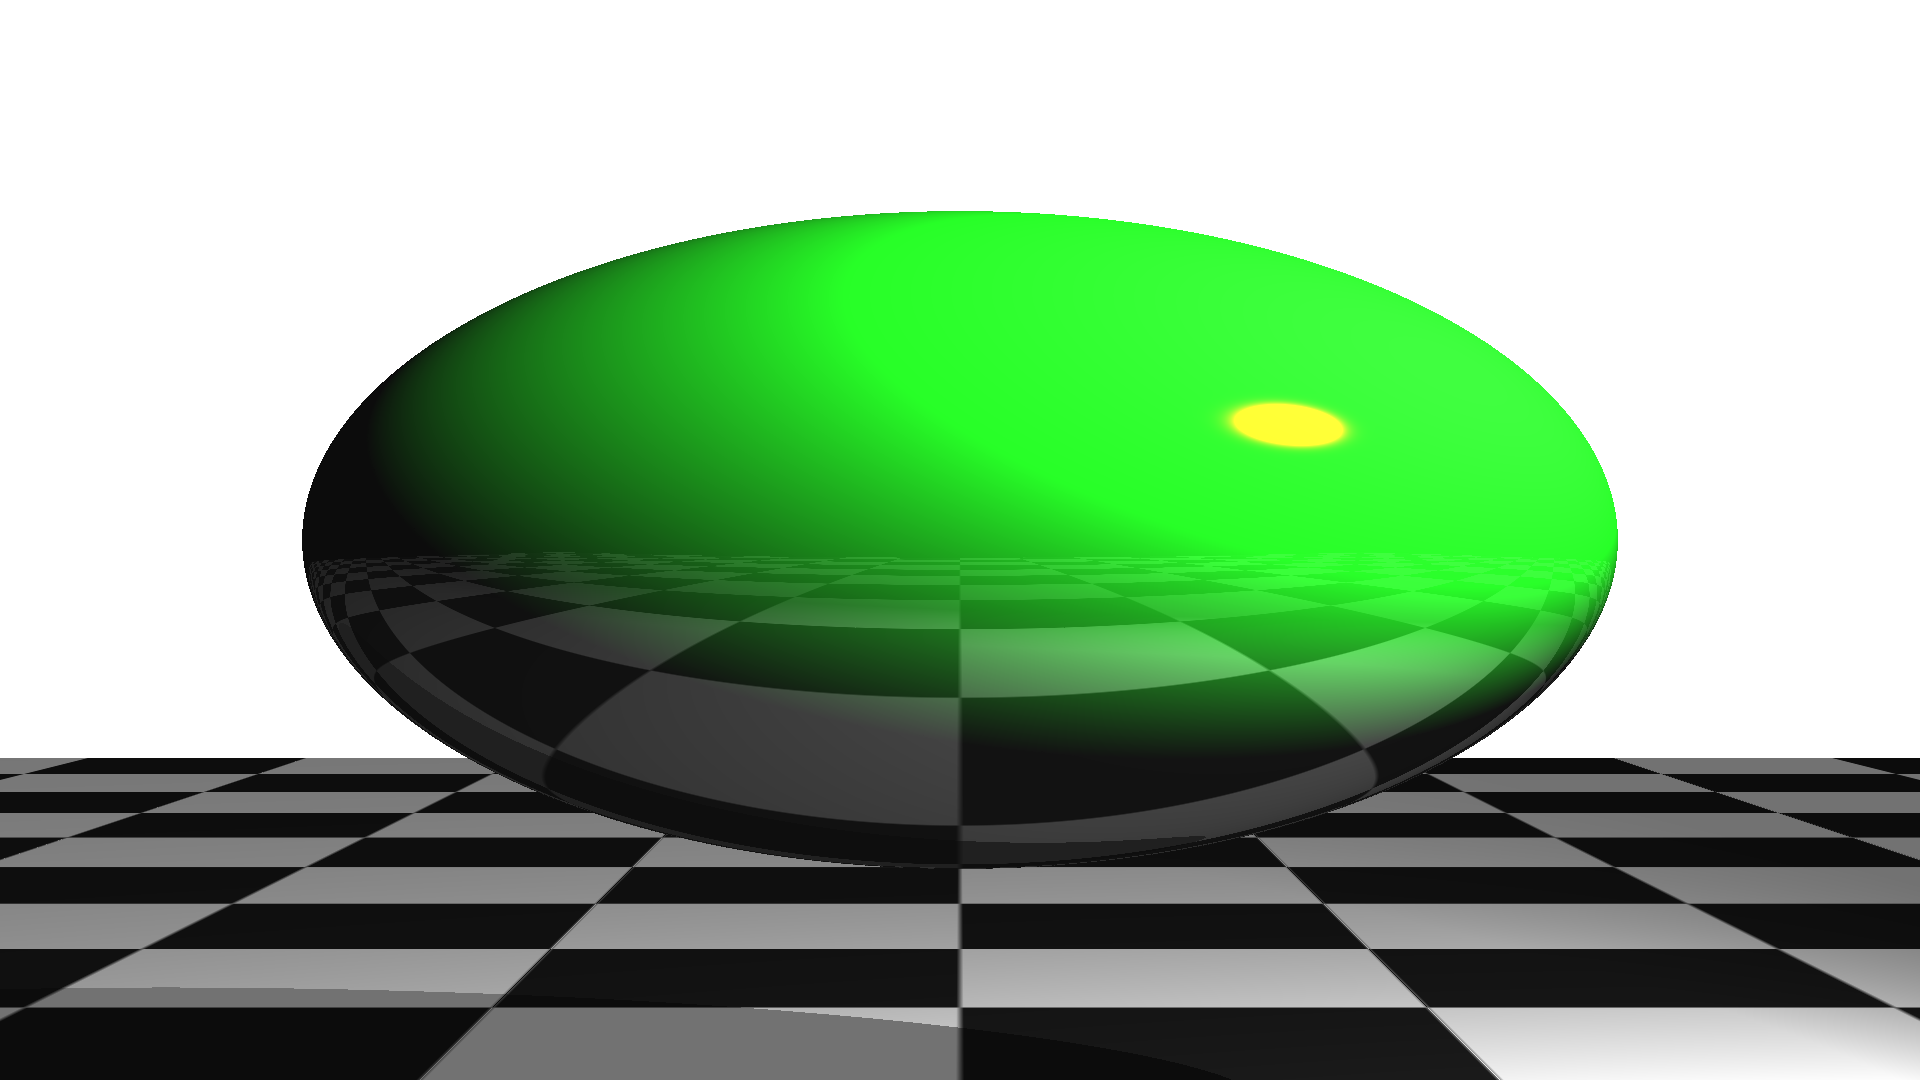
\includegraphics[width=0.3\textwidth]{chapters/ch3/img/reflection/ts_ks_06_exp_1024_eta_133_k_10.png}}

\caption[Powierzchnie odbijające w modelu Torrance'a-Sparrowa]{Powierzchnie odbijające w modelu Torrance'a-Sparrowa. Obrazy w górnym wierszu odpowiadają dielektrykom~($k=0$) o współczynniku załamania (od lewej do prawej) $\eta\in\lbrace 1,33; 1,66; 2,00 \rbrace$. W dolnym wierszu przedstawione zostały przewodniki o~$k\in\lbrace 0,2; 0,6; 1,0 \rbrace$ i $\eta = 1,33$}
\label{ch3:img:reflection_types_ts}
\end{figure}


\item \underline{Teksturowanie powierzchni}

Teksturowanie powierzchni pozwala uatrakcyjnić wizualnie obiekty bez konieczności zwiększania ich złożoności geometrycznej poprzez nadanie punktom znajdującym się na obiekcie odpowiednich kolorów\footnote{Tak naprawdę tekstura może być odpowiedzialna nie tylko za nadanie konkretnego koloru obiektowi, ale może również modulować wektory normalne, współczynniki załamania oraz wiele innych parametrów mających wpływ na ostateczny odbiór obiektu przez obserwatora.}. \textsc{ViRay} pozwala nadać obiektowi pożądaną teksturę~(kilka różnych obiektów może współdzielić tę samą teksturę), której dane zapisane są w postaci mapy bitowej albo mapy szarości. W tym drugim przypadku, odcień szarości $\mathtt{mix}\in[0, 1]$ decyduje o stopniu mieszania między dwoma wybranymi przez użytkownika kolorami:
\begin{equation*}
\mathtt{color = color1\cdot mix + color2\cdot\left(1 - mix \right)}.
\end{equation*}

Problem teksturowania sprowadza się do nałożenia dwuwymiarowej mapy pikseli $\mathtt{w}\times\mathtt{h}$ na powierzchnię obiektu trójwymiarowego, który może wprowadzać zniekształcenie w~jej odwzorowaniu. Z tego powodu współrzędne na mapie pikseli transformowane są liniowo do przestrzeni $[u, v] \in [0, 1]^2$~(rysunek~\ref{ch3:img:texture_mapping}), zaś współrzędne punktu przecięcia promienia z obiektem w przestrzeni obiektu $\vec{p}'\in[-1, 1]^3$ poddawane są innej~(w~ogólnym przypadku nieliniowej) transformacji do przestrzeni $[u, v]$. 


\addimage{chapters/ch3/img/texture_mapping.png}{width=0.85\textwidth}{Transformacja pozycji piksela z przestrzeni tekstury do współrzędnych $[u, v] \in [0, 1]^2$. Tekstura na podstawie~\cite{EARTH_NASA}}{Transformacja pozycji piksela do współrzędnych u, v}{ch3:img:texture_mapping}

Najprostszym sposobem transformacji współrzędnych punktu $\vec{p}'$ do $[u,v]$ jest transformacja liniowa zwana \textit{mapowaniem prostokątnym}:
\begin{align*}
u &= \frac{p_x' + 1}{2},\\
v &= \frac{p_z' + 1}{2}.
\end{align*}
Dostępność dodatkowych trybów mapowania w \textsc{ViRay}'u jest sterowana poprzez przełącznik \texttt{ADVANCED\_TEXTURE\_MAPPING\_ENABLE}. Definicja ta daje dostęp do odwzorowania \textit{cylindrycznego}:
\begin{align*}
u &= \frac{\phi}{2\pi} = \frac{\arctan\frac{p_x'}{p_z'}}{2\pi},\\
v &= \frac{p_y' + 1}{2}
\end{align*} 
oraz \textit{sferycznego}:
\begin{align*}
u &= \frac{\phi}{2\pi} = \frac{\arctan\frac{p_x'}{p_z'}}{2\pi},\\
v &= 1 - \frac{\theta}{\pi} = 1 - \frac{\arccos p_y'}{\pi}.
\end{align*} 

Wpływ trzech wymienionych powyżej trybów na finalne odwzorowanie tekstury na~powierzchni różnych obiektów został przedstawiony na rysunku~\ref{ch3:img:texture_proj}.

\begin{figure}[H]
\centering
\subfigure{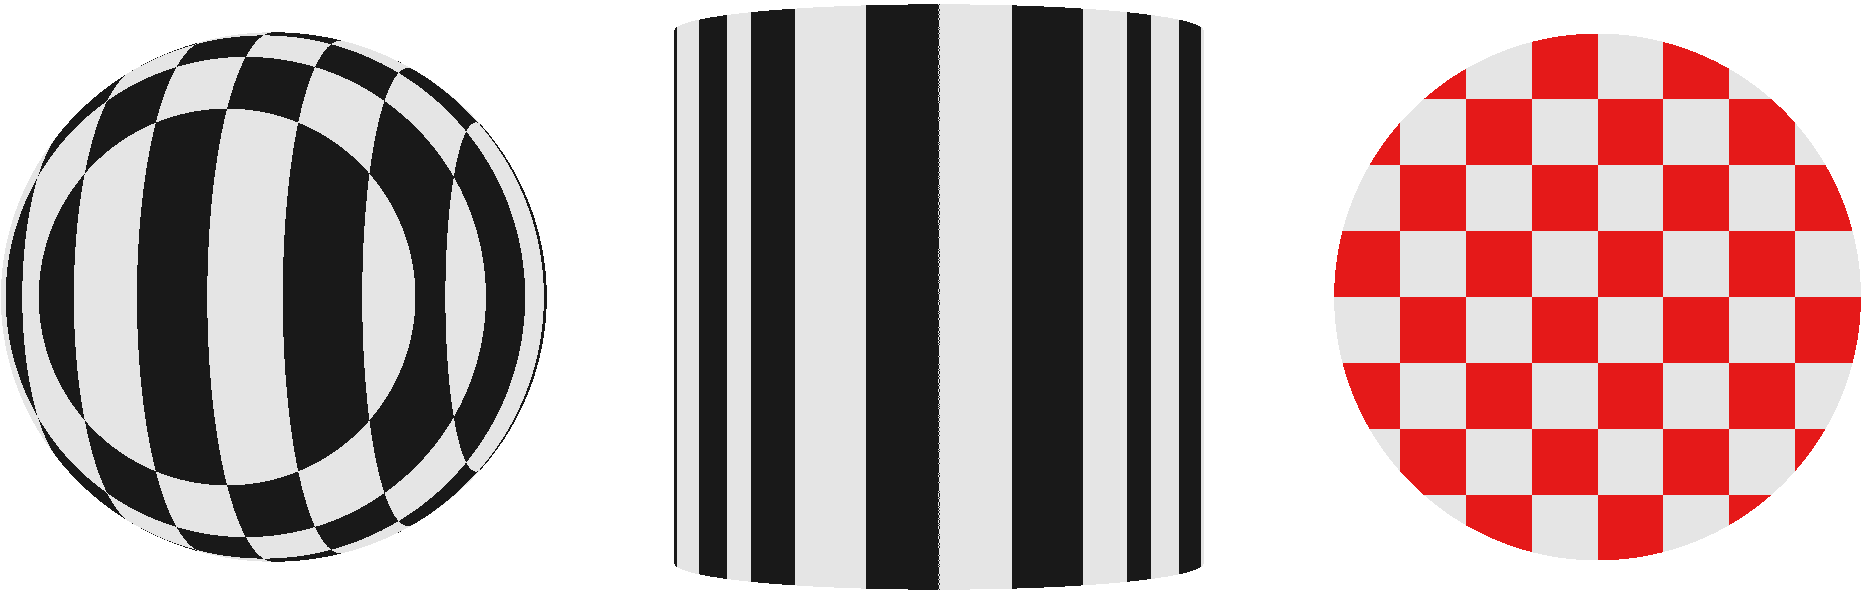
\includegraphics[width=0.55\textwidth]{chapters/ch3/img/texture_proj/planar.png}}
\subfigure{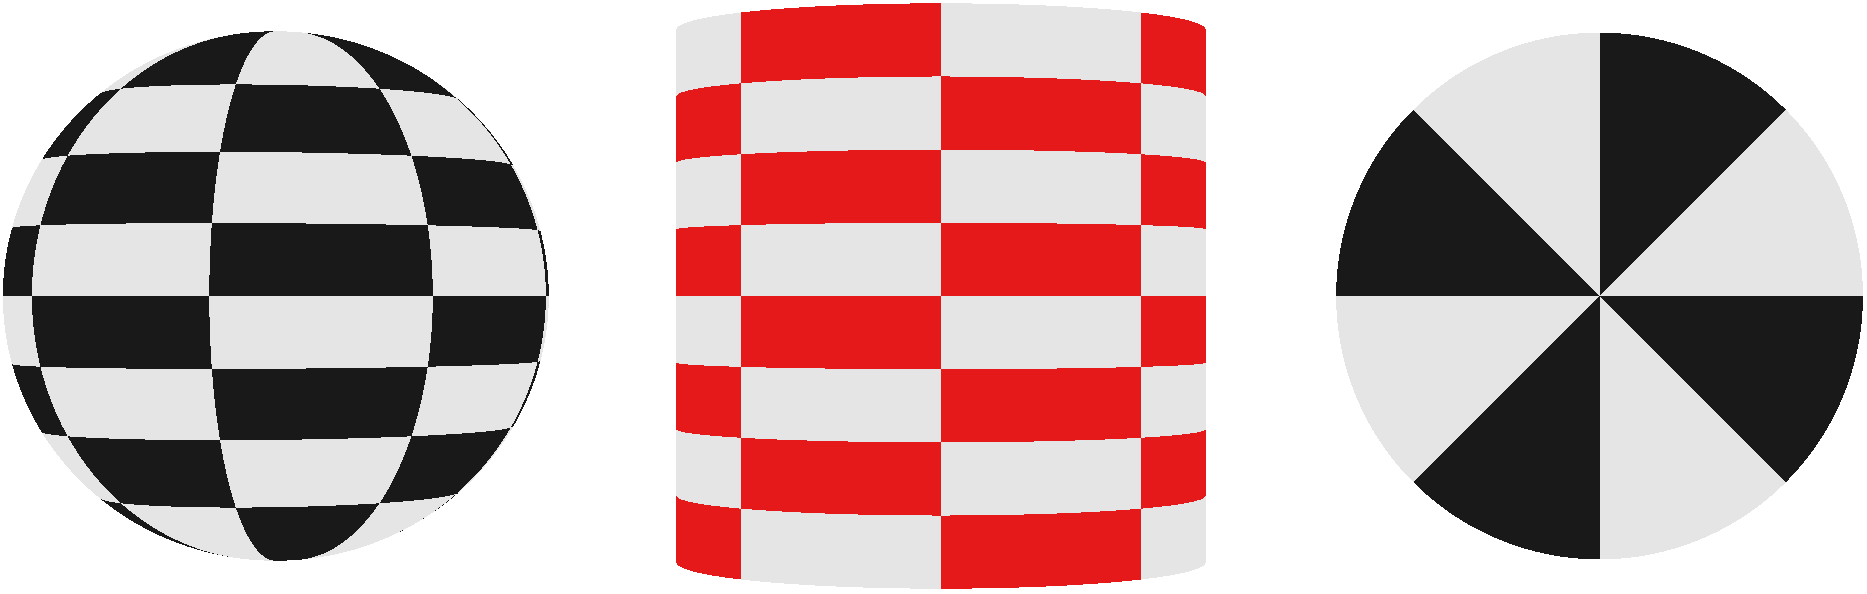
\includegraphics[width=0.55\textwidth]{chapters/ch3/img/texture_proj/cylindrical.png}}
\subfigure{
\includegraphics[width=0.55\textwidth]{chapters/ch3/img/texture_proj/spherical.png}}

\caption[Efekt nałożenia tekstury na różne typy obiektów w funkcji rodzaju zastosowanego mapowania]{Efekt nałożenia identycznej tekstury na różne typy obiektów w funkcji rodzaju zastosowanego mapowania. Od góry: mapowanie prostokątne, cylindryczne i sferyczne}
\label{ch3:img:texture_proj}
\end{figure}



Z zastosowaniem odwzorowania cylindrycznego oraz sferycznego wiąże się konieczność obliczenia odpowiednich kątów na podstawie współrzędnych punktu $\vec{p}'$ z użyciem funkcji cyklometrycznych. Wykorzystanie w tym celu wprost funkcji \texttt{hls::atan2()} oraz \texttt{hls::acos()} dostarczanych wraz z Vivado HLS rodzi jednak kłopoty związane z użyciem przez nie dużej ilości zasobów układu~(tabela~\ref{ch3:tab:atan_acos}), co w praktyce mogłoby oznaczać niemożliwość implementacji odwzorowania cylindrycznego oraz sferycznego w~końcowym systemie śledzenia promieni. Chcąc temu zaradzić \textsc{ViRay} może korzystać z~obliczeń przybliżonych w celu znalezienia aproksymacji wartości funkcji \texttt{atan2()} oraz \texttt{acos()}. Są to odpowiednio \texttt{ViRayUtils::Atan2()} oraz \texttt{ViRayUtils::Acos()}, które włączane są poprzez definicje \texttt{FAST\_ATAN2\_ENABLE} oraz \texttt{FAST\_ACOS\_ENABLE}.

% PORÓWNANIE Z WERSJĄ HLS, GDZIE JEST TYLKO TA JEDNA FUNKCJA ATAN/ACOS
%\begin{table}[]
%\centering
%\caption{My caption}
%\label{my-label}
%\begin{tabular}{|r|c|c|c|c|}
%\hline
%\multicolumn{1}{|l|}{}       & \textbf{BRAM} & \textbf{DSP} & \textbf{FF} & \textbf{LUT} \\ \hline
%\texttt{ViRayUtils::Atan2()} & 0             & 5            & 1153        & 2064         \\ \hline
%\texttt{hls:atan2()}         & 4             & 2            & 1512        & 4166         \\ \hline
%\texttt{ViRayUtils::Acos()}  & 1             & 8            & 920         & 1785         \\ \hline
%\texttt{hls::acos()}         & 0             & 7            & 1721        & 3136         \\ \hline
%\end{tabular}
%\end{table}

\begin{table}[H]
\centering
\caption[Wykorzystanie zasobów sprzętowych układu KCU116 przez poszczególne implementacje funkcji cyklometrycznych]{Raportowane wykorzystanie zasobów sprzętowych układu KCU116 przez poszczególne implementacje funkcji cyklometrycznych. Funkcje biblioteczne \texttt{hls::atan2()} oraz \texttt{hls::acos()} dające najdokładniejsze wyniki wymagają dużej ilości zasobów do ich fizycznej implementacji~(zwłaszcza FF oraz LUT). Zaproponowane implementacje przybliżone \texttt{ViRayUtils::Atan2()} oraz \texttt{ViRayUtils::Acos()} wymagają o wiele mniej logiki układu, zachowując przy tym dokładność wystarczającą podczas teksturowania obiektów}
\label{ch3:tab:atan_acos}
\begin{tabular}{|r|c|c|c|c|}
\hline
\multicolumn{1}{|l|}{}       & \textbf{BRAM} & \textbf{DSP} & \textbf{FF} & \textbf{LUT} \\ \hline\hline

\texttt{hls::atan2()}         & 0             & 2            & 12713       & 16742        \\ \hline
\texttt{hls::acos()}         & 0             & 50           & 12022       & 8038         \\ \hline\hline
\texttt{ViRayUtils::Atan2()} & 0             & 5            & 1153        & 2064         \\ \hline
\texttt{ViRayUtils::Acos()}  & 1             & 8            & 920         & 1785         \\ \hline

\end{tabular}
\end{table}


\begin{itemize}
\item \texttt{ViRayUtils::Atan2()}

Funkcja ta opiera swoje działanie na następującej obserwacji~\cite{ATAN_APPROX}:

\begin{equation}
\arctan(z)\approx 0,9724z - 0,1919z^3,\qquad z=\frac{y}{x}\in[-1, 1]
\end{equation}
oraz tożsamości:
\begin{equation}
\arctan(z) = \frac{\pi}{2} - \arctan\left(z^{-1}\right), \mathrm{gdy} \left| z \right| > 1
\end{equation}

\begin{figure}[H]
\centering
\subfigure{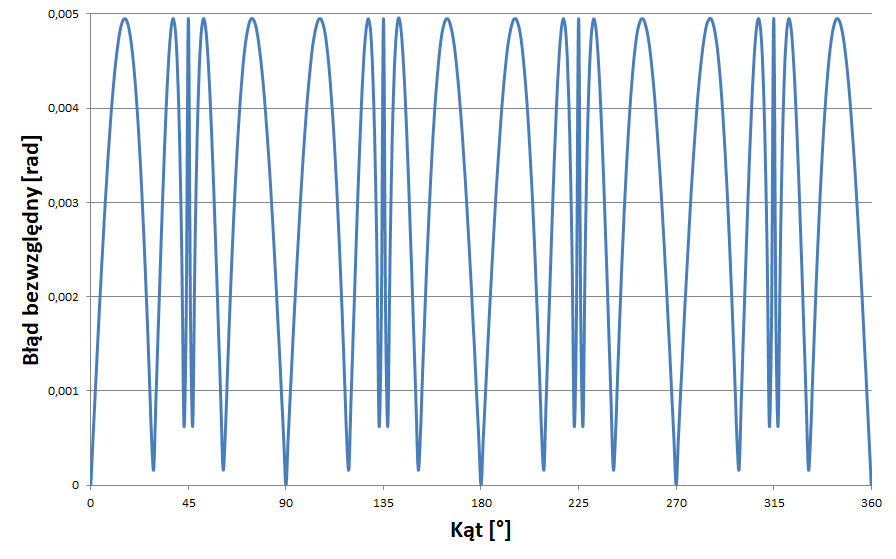
\includegraphics[width=0.8\textwidth]{chapters/ch3/img/atan2_error.png}}
\subfigure{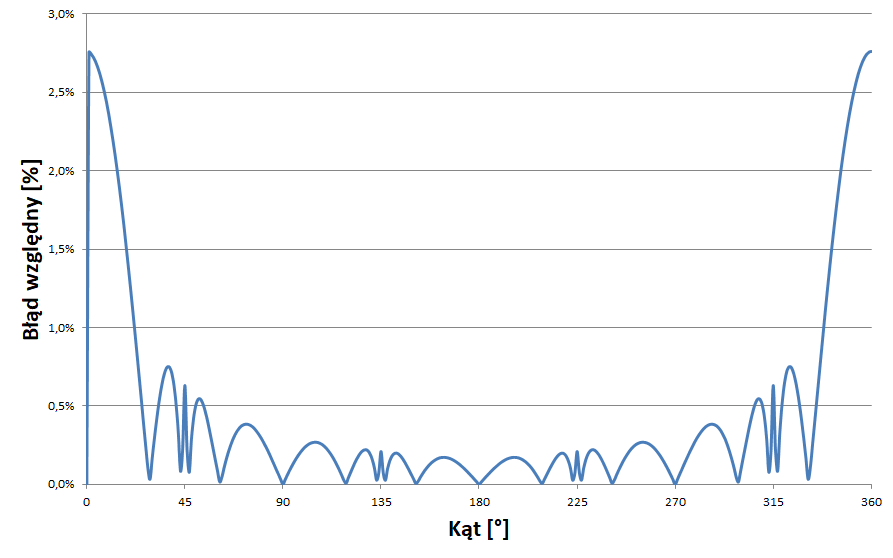
\includegraphics[width=0.8\textwidth]{chapters/ch3/img/atan2_relative_error.png}}
\caption[Błąd bezwzględny oraz względny generowany przez przybliżoną implementację funkcji \texttt{atan2()}]{Błąd bezwzględny oraz względny generowany przez przybliżoną implementację funkcji \texttt{atan2()}. Maksymalny błąd wynosi $0,00496\ \mathrm{rad}$, co przekłada się w najgorszym przypadku na odstępstwo od dokładnego wyniku równe 2,8 \%. Różnice te praktycznie nie wpływają na sposób odwzorowania tekstury na powierzchni}
\label{ch3:img:atan2_error}
\end{figure}


\item \texttt{ViRayUtils::Acos()}

W tym przypadku rozwiązanie przybliżone oparte jest o tablicę 33 wartości, będących dokładnymi wynikami funkcji \texttt{acos()} dla równo oddalonych od siebie parametrów $x_i \in [0, 1]$. Dla parametru wejściowego $x'$ następuje określenie najbliższych mu parametrów $x_i$ oraz $x_{i+1}$, dla których znane są dokładne wartości funkcji. Następnie dokonywana jest interpolacja liniowa pomiędzy tymi wartościami, zależna od odległości $x'$ od $x_i$ oraz $x_{i+1}$. W przypadku, gdy $x' < 0$ wykorzystywana jest tożsamość:
\begin{equation}
\arccos(x') = \pi - \arccos(|x'|).
\end{equation}

\begin{figure}[H]
\centering
\subfigure{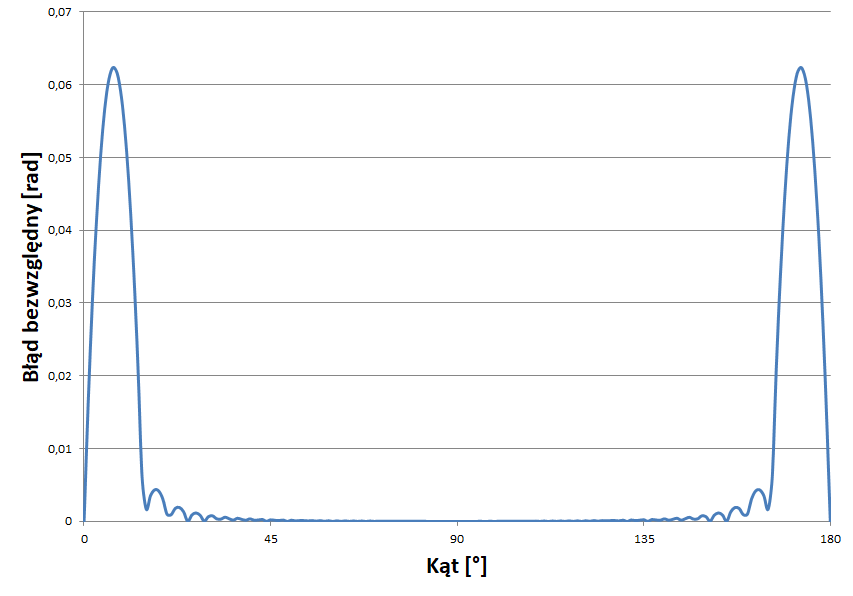
\includegraphics[width=0.8\textwidth]{chapters/ch3/img/acos_error.png}}
\subfigure{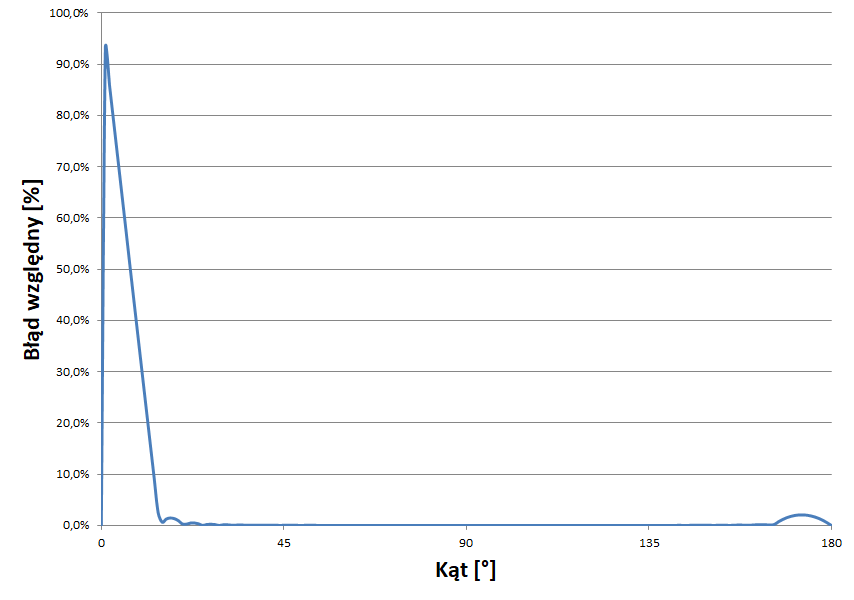
\includegraphics[width=0.8\textwidth]{chapters/ch3/img/acos_relative_error.png}}
\caption[Błąd bezwzględny oraz względny generowany przez przybliżoną implementację funkcji \texttt{acos()}]{Błąd bezwzględny oraz względny generowany przez przybliżoną implementację funkcji \texttt{acos()}. Maksymalny błąd wynosi $0,0624\ \mathrm{rad}$, który występuje w okolicach 0 oraz $\pi$ radianów, a związane jest to z faktem, iż funkcja \texttt{acos()} przejawia tam największe odstępstwa od liniowości~($\frac{\mathrm{d}(\arccos(x))}{\mathrm{d}x} = \frac{1}{\frac{\mathrm{d}\cos(x)}{\mathrm{d}x}} = -\frac{1}{\sin(x)}$). Mimo tej jednej niedogodności, zastosowane przybliżenie sprawdza się podczas teksturowania obiektów}
\label{ch3:img:acos_error}
\end{figure}

\end{itemize}

Algorytmy dokonujące teksturowania pozwalają również dokonywać translacji tekstury oraz jej skalowania poprzez powielanie. Możliwości te zostały zilustrowane na rysunku~\ref{ch3:img:texture_transform}.

\addimage{chapters/ch3/img/texture_proj/texture_transform.png}{width=0.85\textwidth}{Translacja oraz skalowanie tekstury. a) Kwadrat z oryginalną teksturą. b) Tekstura została przesunięta o 0,1 jednostki w lewo oraz 0,2 jednostki w dół. c) Oryginalna tekstura została przeskalowana w taki sposób, że została powielona dwukrotnie w kierunku $u$ oraz trzykrotnie w kierunku $v$~(możliwe są również niecałkowite wartości skali). d) Oryginalny obiekt a) został poddany skalowaniu co wpłynęło również na deformację tekstury}{Translacja oraz skalowanie tekstury}{ch3:img:texture_transform}

Tekstury w \textsc{ViRay}'u są całkowicie przechowywane w pamięci BRAM układu FPGA\footnote{Własność ta wynika z faktu, iż Vivado HLS nie pozwala dokonywać asynchronicznych, względem potoku przetwarzania w module, operacji odczytu danych z pamięci zewnętrznej.

Możliwe jest również poinstruowanie Vivado HLS, aby pamięć tekstur znalazła się w układach UltraRAM za pomocą definicji \texttt{TEXTURE\_URAM\_STORAGE}. Rozwiązanie to jest jednakże niezalecane z uwagi na fakt, iż~bloki UltraRAM są zlokalizowane w układzie FPGA tzn. nie są tak bardzo rozproszone po całym układzie jak~bloki BRAM, w wyniku czego na etapie implementacji dochodzi do nadmiernego stłoczenia, czyli lokalnego przeciążenia sieci połączeń, co prowadzi do niepowodzenia implementacji.

}. Fakt ten wymusza stosowanie tekstur o odpowiednio niskiej rozdzielczości~(standardowo \textsc{ViRay} udostępnia miejsce na $2^{16}$ 32-bitowych wartości, patrz \texttt{TEXT\_PAGE\_SIZE}). W takim wypadku obraz nałożony w sposób bezpośredni na powierzchnię bez odpowiedniej filtracji zostanie poszarpany z wyraźnymi krawędziami pomiędzy pikselami tekstury. Użycie przełącznika \texttt{BILINEAR\_TEXTURE\_FILTERING\_ENABLE} w pliku konfiguracyjnym za cenę rozmycia szczegółów tekstury pozwala wyeliminować wyraźne granice między pikselami~(rysunek~\ref{ch3:img:bilinear_filtering}). 

\addimage{chapters/ch3/img/bilinear_filtering.png}{width=0.8\textwidth}{Algorytm filtracji biliniowej tekstury. Zaznaczony na {\color{red}czerwono} punkt $\vec{p}'$ na~powierzchni obiektu odpowiada środkowemu pikselowi tekstury, jednak nie wypada on w~samym centrum obszaru~(tzw. \textit{centroid} {\color{orange}$\mathbf{c_{(u, v)}}$}). W kierunku $u$ oraz $v$ znajdowane są najbliższe piksele tekstury przylegające do piksela centralnego i najbliższe $\vec{p}'$~(w tym przypadku {\color{orange}$\mathbf{c_{(u-1, v)}}$} oraz {\color{orange}$\mathbf{c_{(u, v-1)}}$}). Kolor tekstury w $\vec{p}'$ obliczony zostaje na podstawie kolorów tychże pikseli i ich wag, zależnych od odległości $\vec{p}'$ od centroidów wzdłuż osi $u$ oraz $v$, jako interpolacja liniowa w kierunku $u$ oraz $v$}{Algorytm filtracji biliniowej tekstury}{ch3:img:bilinear_filtering}

\item \underline{Zapis finalnego koloru piksela - \texttt{SaveColorToBuffer()}}

Zanim finalny kolor piksela zostanie zapisany w buforze ramki, zmiennoprzecinkowy wektor $\mathtt{\overrightarrow{color}}$ przechowujący informację o kolorze zostaje poddany konwersji do 3 8-bitowych wartości \texttt{R}, \texttt{G}, \texttt{B} za pomocą prostej transformacji:

\begin{lstlisting}
unsigned tempColor[3];
for(unsigned i = 0; i < 3; ++i)
{
	// R: i = 0
	// G: i = 1
	// B: i = 2
	if (color[i] > float(1.0))	color[i] = float(1.0);
	tempColor[i] = unsigned(color[i] * 255.0f);
}
\end{lstlisting}
Sprawdzenie warunku w ciele pętli jest konieczne po to, aby wyjściowe wartości składowych koloru nie przekroczyły maksymalnej wartości możliwej do zapisania za pomocą 8 bitów. Konsekwencją tego rozwiązania są tzw. \textit{przepalenia}, czyli obszary, gdzie intensywność którejkolwiek ze składowych w wektorze $\mathtt{\overrightarrow{color}}$ są większe niż 1~(patrz komentarz pod rysunkiem~\ref{ch3:img:blinn_phong}).

Otrzymane w ten sposób wartości są następnie pakowane w jedną 32-bitową wartość reprezentującą finalny kolor piksela przy czym proces ten jest kontrolowany poprzez definicję \texttt{PIXEL\_COLOR\_CONVERSION\_ENABLE}, co zostało pokazane na poniższym schemacie.

\addimage{chapters/ch3/img/color_conversion.png}{width=1.0\textwidth}{Upakowanie danych koloru \texttt{RGB} w 32-bitowej wartości w buforze ramki. Przypadek a) odpowiada sytuacji, gdy \texttt{PIXEL\_COLOR\_CONVERSION\_ENABLE} nie zostało zdefiniowane - wtedy każdy 32-bitowy element bufora ramki przechowuje informacje o wszystkich trzech składowych koloru. W sytuacji b), gdy \texttt{PIXEL\_COLOR\_CONVERSION\_ENABLE} zostało zdefiniowane, każdy 32-bitowy element bufora ramki niesie ze sobą informację o składowej zielonej \texttt{G} - informacje o składowych niebieskiej \texttt{B} i czerwonej \texttt{R} zapisywane są naprzemiennie w kolejnych elementach~(dany piksel posiada albo informację o kanale \texttt{B} albo \texttt{R}), przy czym jako pierwsza występuje składowa \texttt{B}~($n=0$)}{Upakowanie danych koloru \texttt{RGB} w 32-bitowej wartości w buforze ramki}{ch3:img:color_conversion}

Trybu zapisu, który implikuje definicja \texttt{PIXEL\_COLOR\_CONVERSION\_ENABLE}, został stworzony po to, aby na płytce ewaluacyjnej KCU116 w pełnym systemie przetwarzania danych możliwe było bezpośrednie wykorzystanie danych bufora ramki dostarczanych przez \textsc{ViRay} bez konieczności stosowania dodatkowych modułów dokonujących odpowiedniej konwersji danych.

\subsubsection{\textsc{ViRay} - wydajność oraz estymacja wymaganych zasobów}

Dla parametrów modułu \textsc{ViRay} zgodnych z danymi zebranymi w tabeli~\ref{ch3:tab:typedefs}, okresu zegara równego 3,3~ns oraz układu KCU116 raport po syntezie HLS~(w wersji 2017.4) przedstawia się następująco:

\begin{table}[H]
\centering
\caption[Wykorzystanie zasobów układu KCU116 oraz szybkość finalnej wersji modułu \textsc{ViRay}]{Wykorzystanie zasobów układu KCU116 oraz szybkość finalnej wersji modułu \textsc{ViRay}. Dolny wiersz odpowiada sytuacji, gdyby zamiast 32-bitowych liczb zmiennoprzecinkowych \texttt{float} do obliczeń w całym module wykorzystać typ połówkowej precyzji \texttt{half}. Ostatnia kolumna (\textbf{\#}) prezentuje ilość cykli zegara potrzebnych na wykonanie wszystkich zadań związanych z tworzeniem pojedynczej ramki obrazu w rozdzielczości 1920 x 1080 pikseli~(Full HD) oraz przeliczenie tej wartości na czas przetwarzania w milisekundach}
\label{ch3:tab:viray_util}
\begin{tabular}{|r|c|c|c|c|c|}
\hline
\multicolumn{1}{|l|}{} & \textbf{BRAM}                                           & \textbf{DSP}                                            & \textbf{FF}                                                & \textbf{LUT}                                               & \textbf{\#}                                                  \\ \hline
\texttt{float}         & \begin{tabular}[c]{@{}c@{}}164\\ (17,1\%)\end{tabular} & \begin{tabular}[c]{@{}c@{}}911\\ (50,0\%)\end{tabular} & \begin{tabular}[c]{@{}c@{}}348999\\ (80,4\%)\end{tabular} & \begin{tabular}[c]{@{}c@{}}173126\\ (79,8\%)\end{tabular} & \begin{tabular}[c]{@{}c@{}}16765083\\ (55,3 ms)\end{tabular} \\ \hline\hline
\texttt{half}          & \begin{tabular}[c]{@{}c@{}}170\\ (17,7\%)\end{tabular} & \begin{tabular}[c]{@{}c@{}}835\\ (45,8\%)\end{tabular} & \begin{tabular}[c]{@{}c@{}}176873\\ (40,8\%)\end{tabular} & \begin{tabular}[c]{@{}c@{}}111854\\ (51,6\%)\end{tabular} & \begin{tabular}[c]{@{}c@{}}16734245\\ (55,2 ms)\end{tabular} \\ \hline
\end{tabular}
\end{table}

Podane powyżej wartości odnoszą się do ramki obrazu 1920~x~1080 pikseli (ok.~2,07~mln pikseli), generowanej przez moduł, który jest implementowalny w fizycznym układzie FPGA. Wynika z nich, iż wymagania dotyczące minimalnej płynności~(tj.~100~ms na~ramkę obrazu) oraz rozdzielczości~(1~mln pikseli) zostały zrealizowane. Ponadto czas generowania obrazu jest stały i zadany przez zastosowaną konfigurację. Jest to~niewątpliwie zasługa poczynionych optymalizacji algorytmów oraz uproszczeń, dzięki którym możliwe jest generowanie kolejnych pikseli obrazu z interwałem równym 8 cykli zegara (\texttt{DESIRED\_INNER\_LOOP\_II}).

W tabeli~\ref{ch3:tab:viray_util} została również umieszczona informacja dotycząca sytuacji, gdyby wszystkie obliczenia \textsc{ViRay} przeprowadzał z użyciem typu \texttt{half} zamiast \texttt{float}. Mimo iż~raportowana przez Vivado HLS utylizacja zasobów jest tylko estymacją, różnice są na~tyle duże, iż można założyć, że zaoszczędzone elementy układu FPGA można byłoby przeznaczyć do implementacji dodatkowych funkcjonalności bądź zmniejszenia interwału między pikselami. Z drugiej strony takie zmniejszenie precyzji nie pozostawałoby bez wpływu na jakość generowanej informacji wizualnej~(rysunek~\ref{ch3:img:float_vs_half}).

W tym miejscu należy wytknąć twórcom Vivado~HLS niekonsekwencję związaną z dostępnymi w Vivado~HLS typami danych. Skoro typy całkowitoliczbowe oraz stałopozycyjne mogą zostać zdefiniowane przez użytkownika w dowolny sposób, z dowolną ilością bitów,  niezrozumiałym jest dostęp do jedynie podstawowych typów zmiennoprzecinkowych tj. \texttt{half}, \texttt{float} oraz \texttt{double}. Obecność typów zmiennoprzecinkowych dowolnej precyzji o rozmiarze pomiędzy 16 a 32 bitami pozwoliłaby przeprowadzić dodatkowe eksperymenty i zoptymalizować \textsc{ViRay} w jeszcze większym stopniu niż możliwe jest to obecnie.

\begin{figure}[H]
\centering
\subfigure{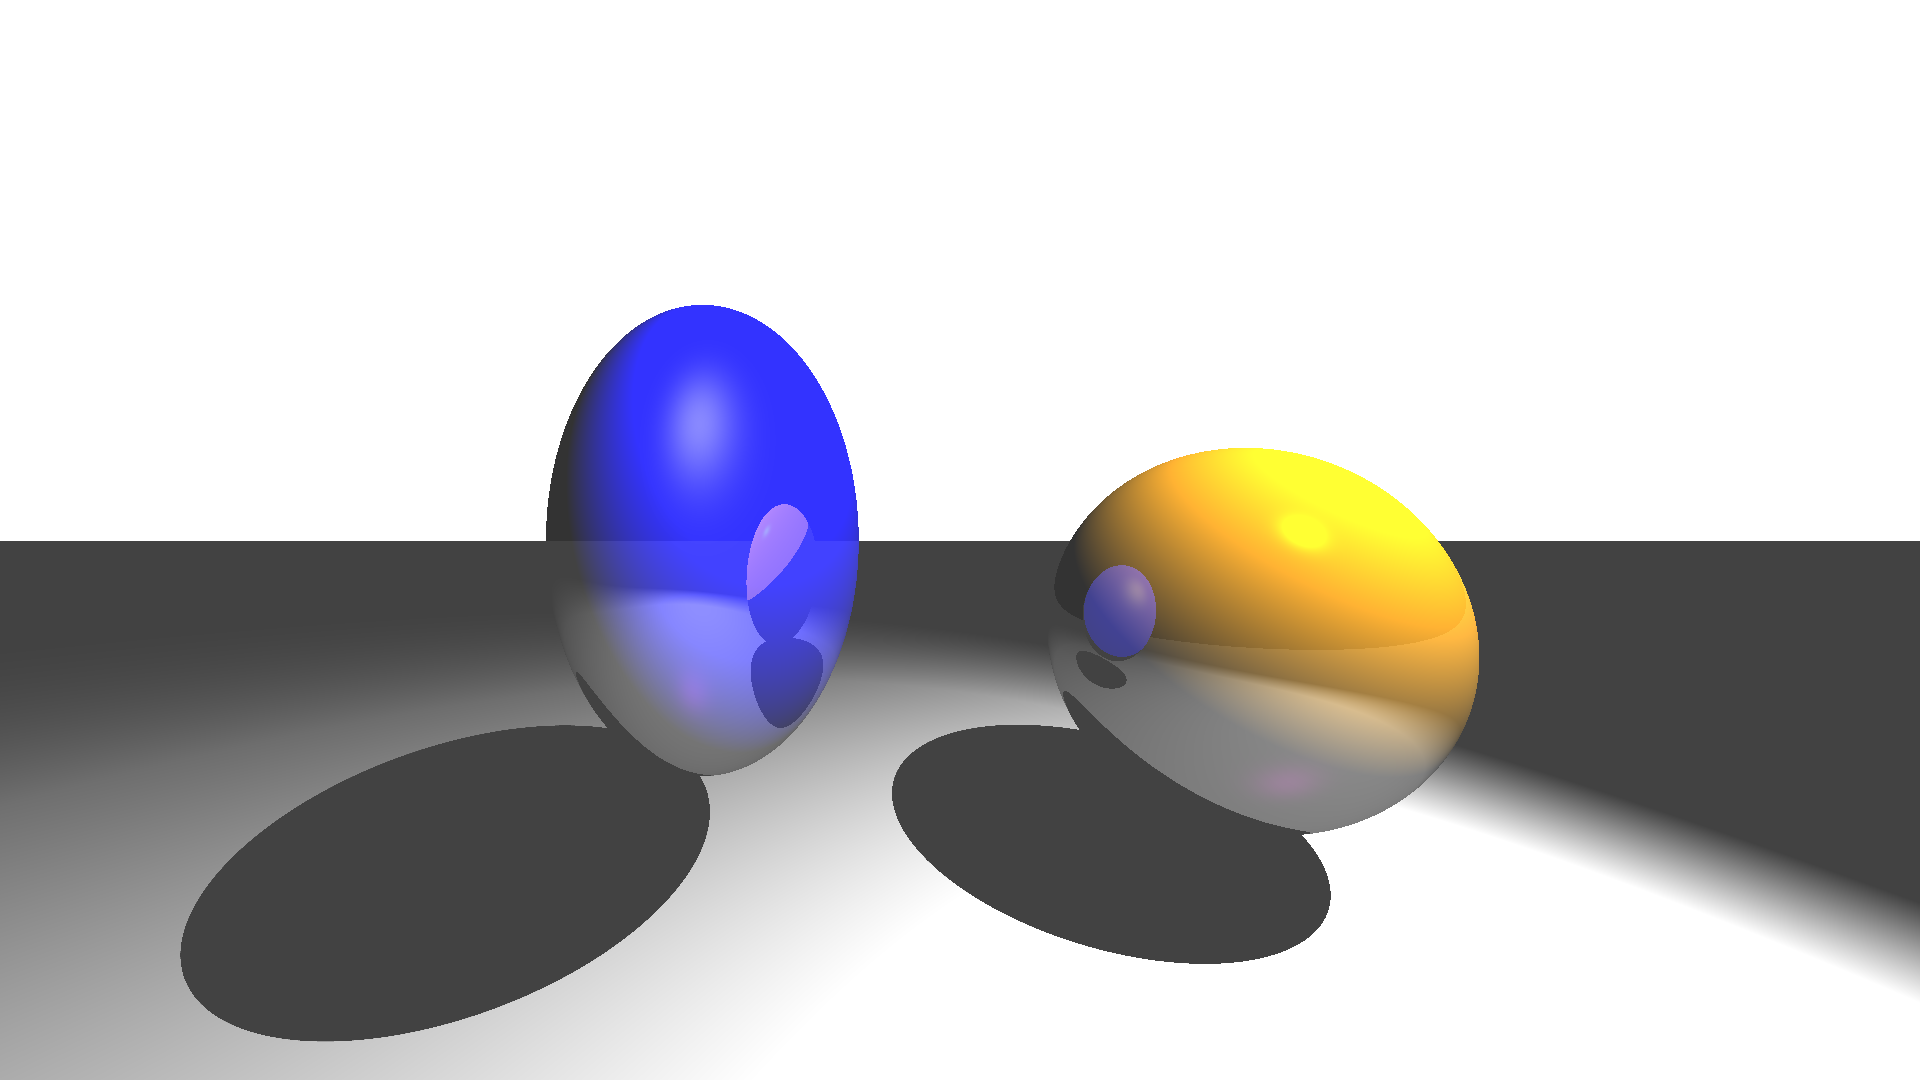
\includegraphics[width=0.85\textwidth]{chapters/ch3/img/float_half/output_refl_full.png}}
\subfigure{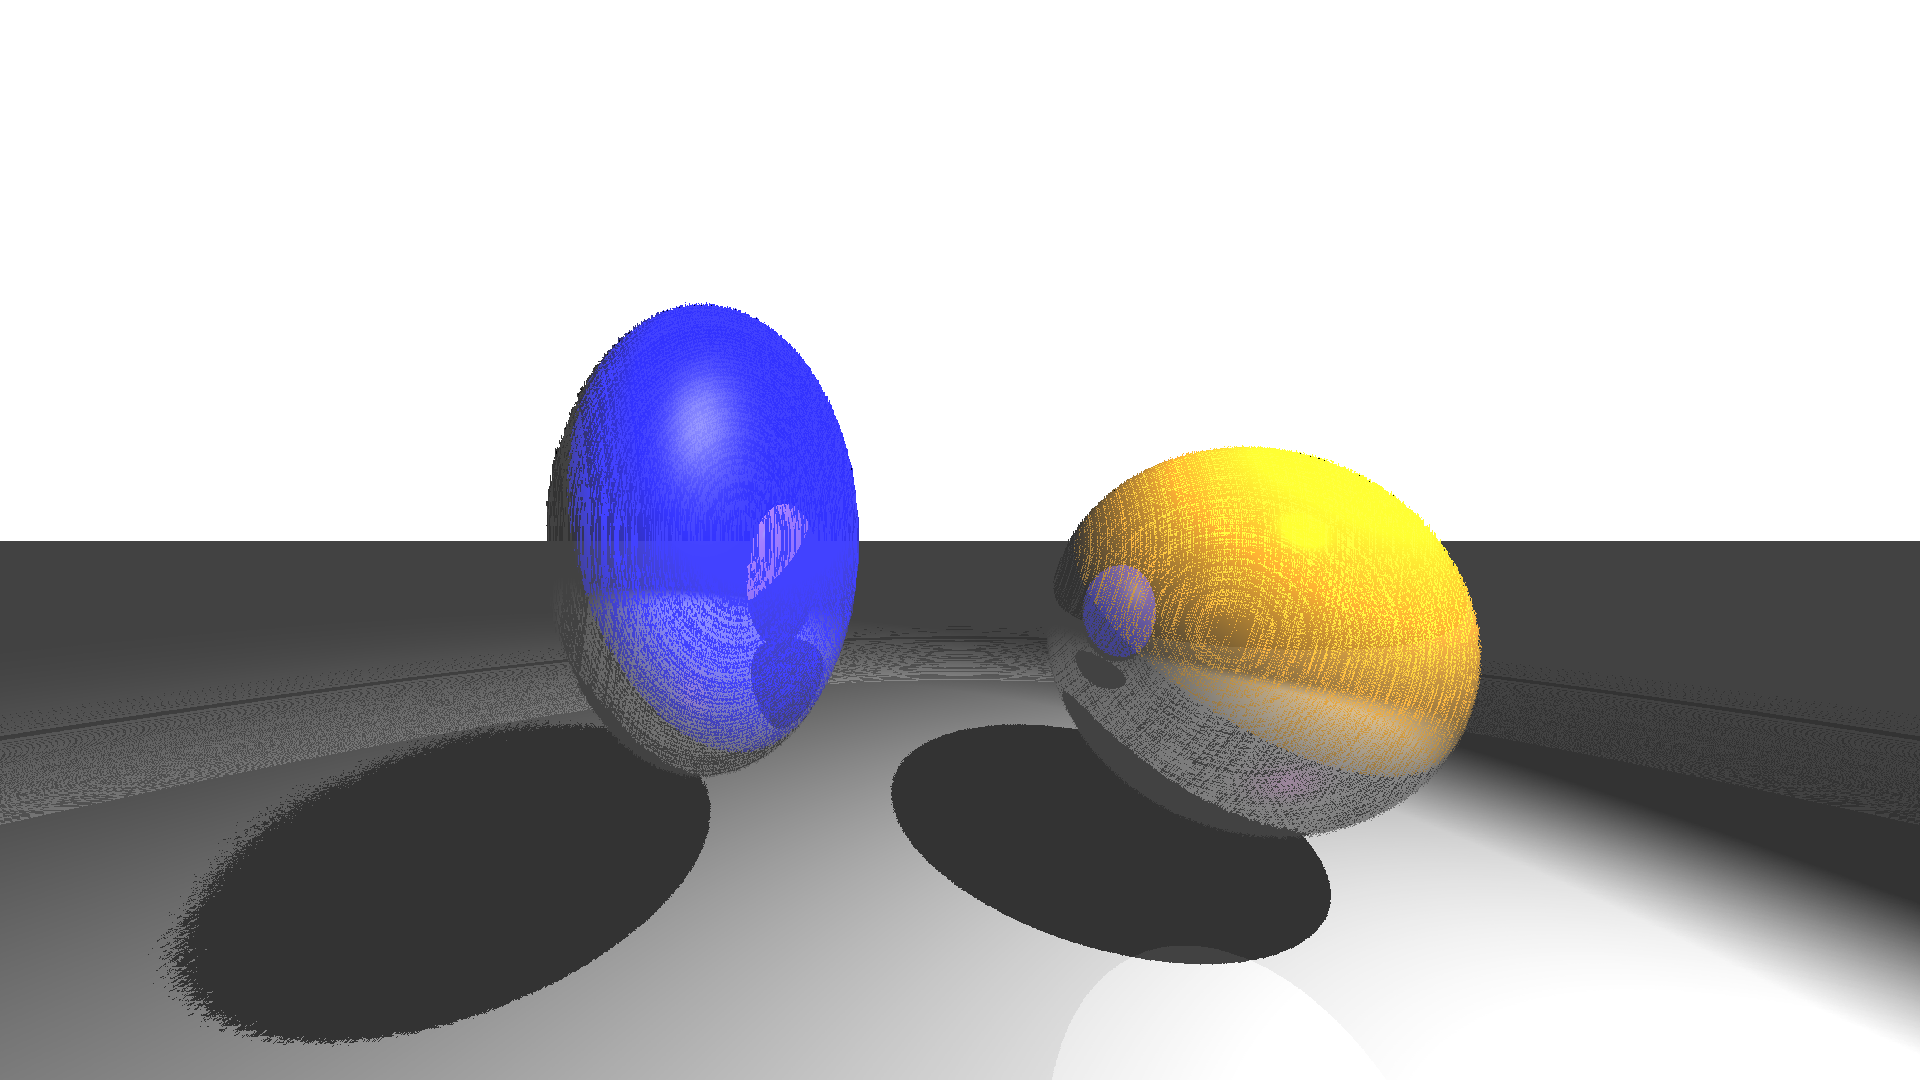
\includegraphics[width=0.85\textwidth]{chapters/ch3/img/float_half/output_refl_half.png}}
\caption[Porównanie obrazów wygenerowanych przez wczesną wersję modułu \textsc{ViRay} za pomocą liczb o różnej precyzji]{Porównanie obrazów wygenerowanych przez wczesną wersję modułu \textsc{ViRay}. Ta~sama scena została wygenerowana z użyciem pełnej~(góra) oraz połówkowej~(dół) precyzji obliczeń zmiennoprzecinkowych. W tym drugim przykładzie uwidaczniają się artefakty wynikające ze zbyt niskiej precyzji obliczeń, przy czym zmiana wartości parametru \texttt{CORE\_BIAS} nie dawała zauważalnej poprawy rezultatów}
\label{ch3:img:float_vs_half}
\end{figure}
\end{enumerate}

\subsubsection{\textsc{ViRay} - wpływ zastosowanej konfiguracji na złożoność sceny}
Przedstawione do tej pory obrazy tworzone za pomocą \textsc{ViRay}'a demonstrowały tylko pewne elementy funkcjonalności finalnego modułu ważne do zilustrowanie danego zagadnienia. Poniższa seria wygenerowanych obrazów~(rysunek~\ref{ch3:img:complexity}) nie tylko pokazuje działanie \textsc{ViRay}'a w bardziej złożonej scenie, ale również pozwala poznać wpływ większości kluczowych parametrów na jej ostateczny wygląd. Wszystkie te obrazy, tak samo jak reszta w tym podrozdziale, są wynikiem działania środowiska symulacyjnego, które powstawały dzięki włączaniu kolejnych funkcjonalności, a ich numery zaczynają się od 1 i rosną od lewej do prawej, z góry na dół.
\begin{enumerate}
\item Scena oświetlona tylko poprzez globalne światło otoczenia \texttt{AMBIENT\_COLOR\_ENABLE}.
\item Włączenie światła rozproszonego \texttt{DIFFUSE\_COLOR\_ENABLE}.
\item Dodanie czynnika \texttt{SPECULAR\_HIGHLIGHT\_ENABLE} związanego z generowaniem rozbłysków zwierciadlanych.
\item Umożliwienie rzucania cieni przez obiekty \texttt{SHADOW\_ENABLE}.
\item Nałożenie tekstur na obiekty \texttt{TEXTURE\_ENABLE}.
\item Filtracja biliniowa tekstur \texttt{BILINEAR\_TEXTURE\_FILTERING\_ENABLE} - sprawia, że tekstura na centralnym obiekcie staje się znacznie gładsza.
\item Rozpoczęcie generowania odbić na obiektach \texttt{RAYTRACING\_DEPTH = 2} - konfiguracja domyślna.
\item \texttt{RAYTRACING\_DEPTH = 3}.
\item \texttt{RAYTRACING\_DEPTH = 4}.
\item \texttt{RAYTRACING\_DEPTH = 10}.
\end{enumerate}

Największy skok w jakości uzyskiwany jest w momencie, gdy zaczynają być generowane cienie~(4), które pozwalają znacznie łatwiej zorientować się w przestrzennej relacji między obiektami a światłem oraz po włączeniu możliwości generowania promieni rozproszonych~(7). Dalsze zwiększanie parametru związanego z głębokością śledzenia promieni dodaje kolejne detale na powierzchniach obiektów, jednak każdy kolejny promień wnosi coraz mniejszy wkład do końcowego efektu, gdyż $0 \leq r_{l-1} \leq 1$~(patrz równanie~\eqref{ch3:eq:total_radiance}), w wyniku czego różnice między obrazami dla \texttt{RAYTRACING\_DEPTH = 4} oraz \texttt{RAYTRACING\_DEPTH = 10} są niewielkie.

Wartym uwagi parametrem jest również czas, w jakim wygenerowany został obraz (7). Ten odpowiada konfiguracji domyślnej \textsc{ViRay}'a dostosowanej do działania na układzie KCU116 w czasie rzeczywistym. Na komputerze wyposażonym w procesor Intel~Core~i5 4690K działającym z częstotliwością 3,9~GHz, czas oczekiwania na wynik symulacji, będącej wykonywalnym jednowątkowym programem napisanym w języku C++, wynosi ok.~67,6~s, czyli jest 3 rzędy wielkości dłuższy, niż gdyby ta sama scena była generowana bezpośrednio w układzie FPGA za pomocą stworzonego modułu~($\frac{67,6~\mathrm{s}}{55,3~\mathrm{ms}}\approx 1222$). 

\begin{figure}[H]
\centering
\subfigure{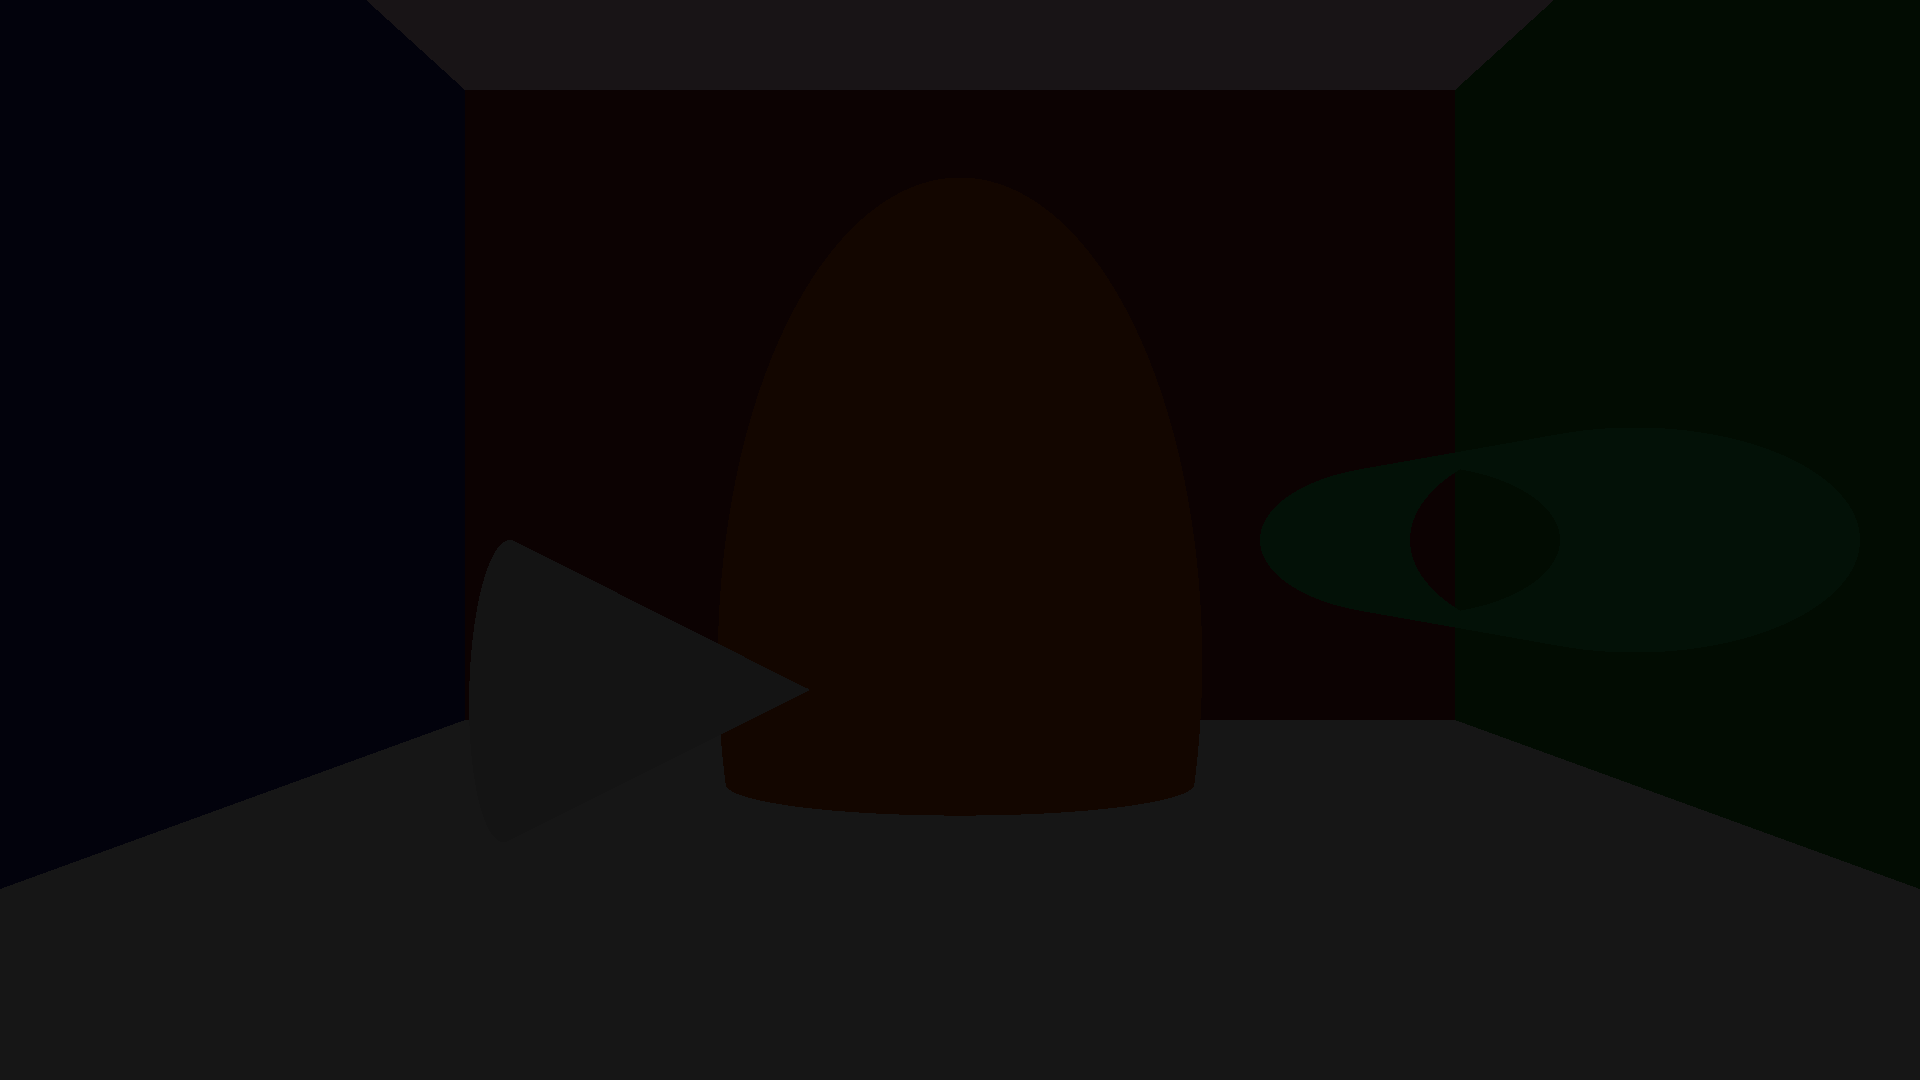
\includegraphics[width=0.45\textwidth]{chapters/ch3/img/complexity/0.png}}
\subfigure{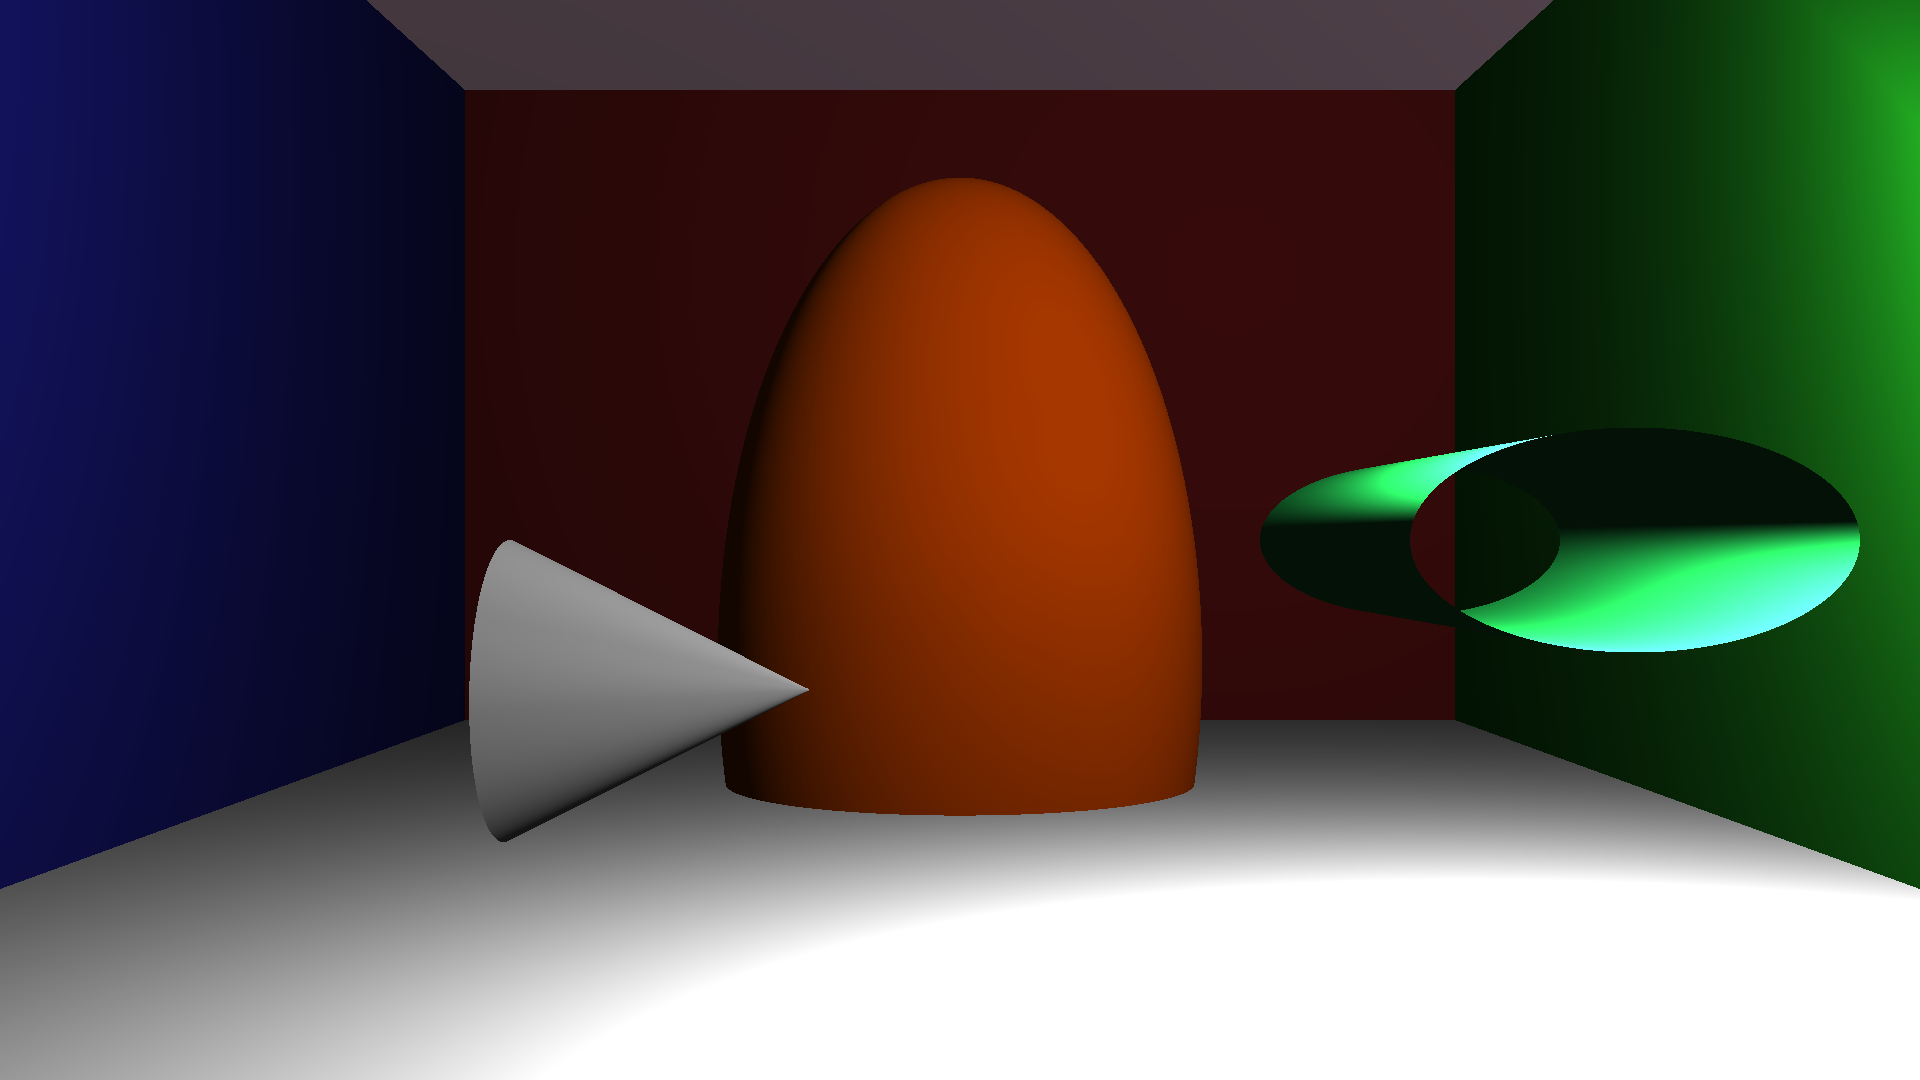
\includegraphics[width=0.45\textwidth]{chapters/ch3/img/complexity/1.png}}

\subfigure{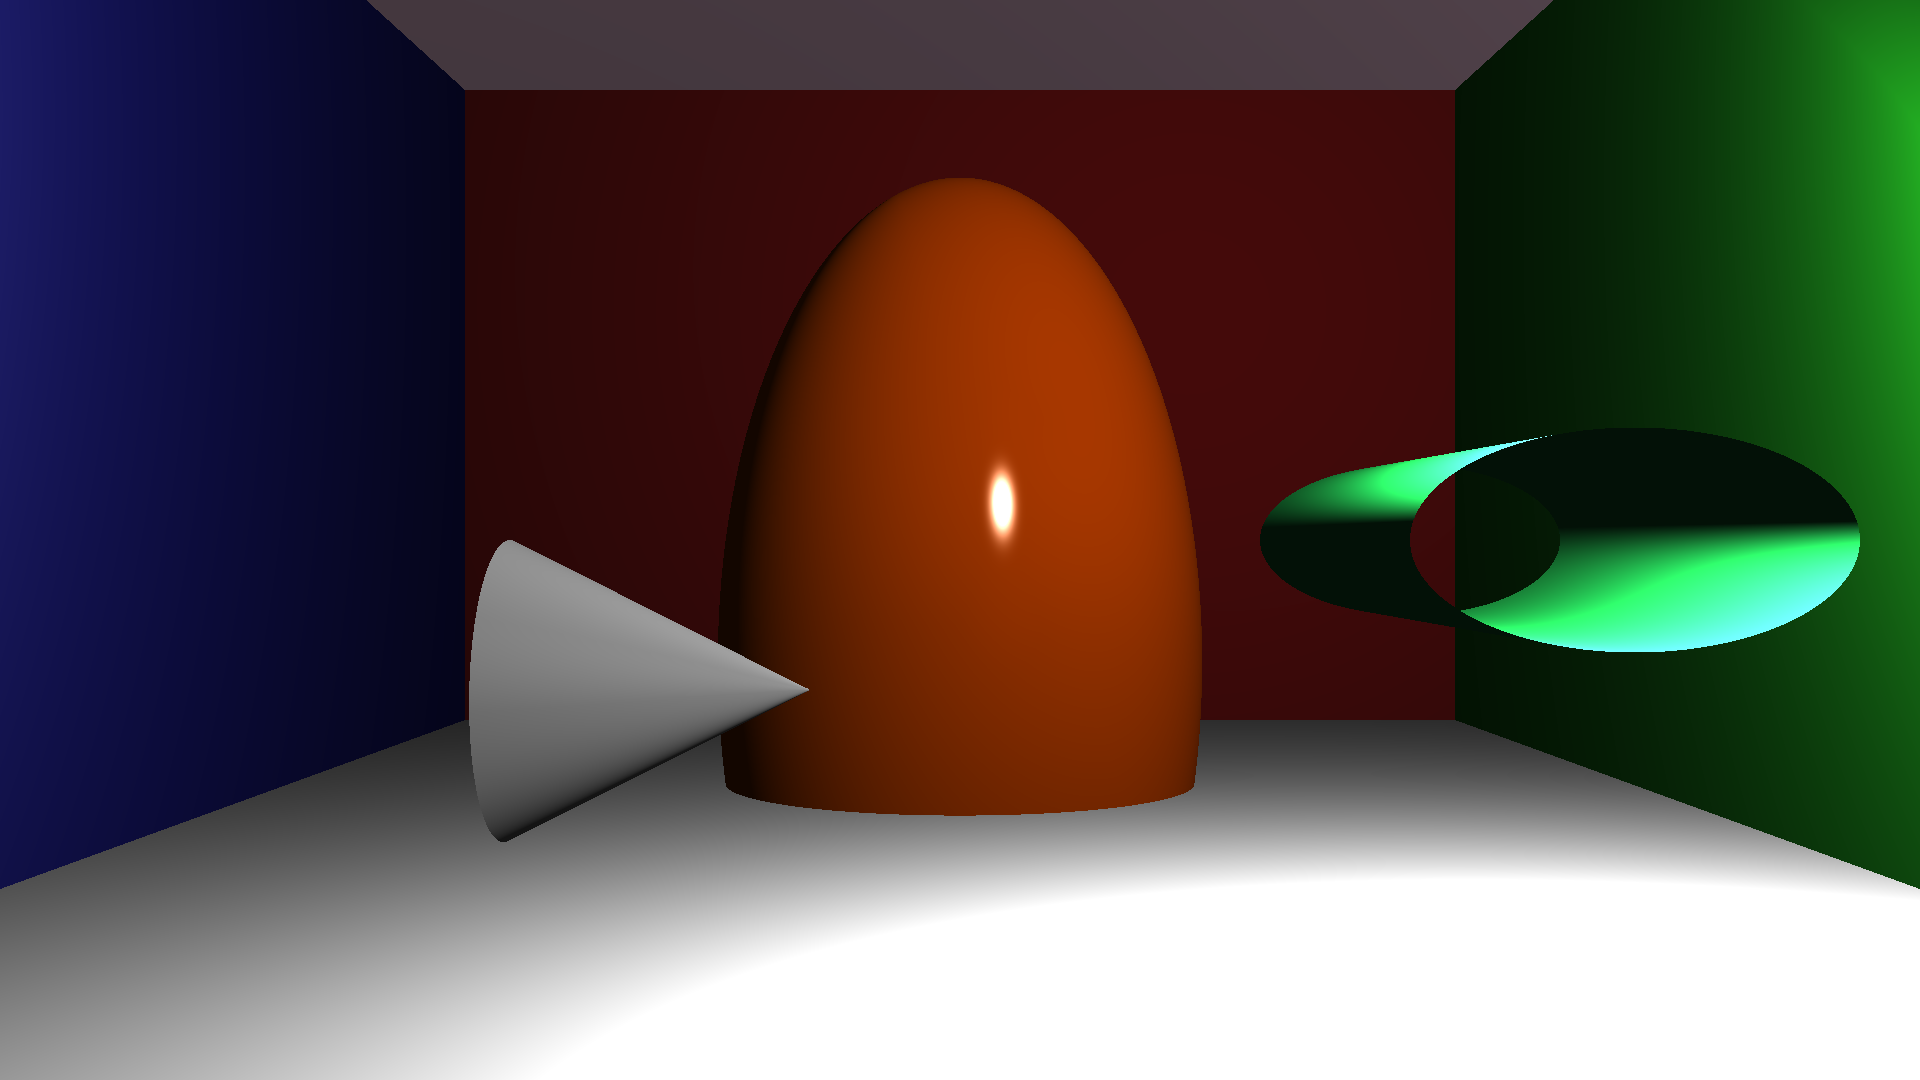
\includegraphics[width=0.45\textwidth]{chapters/ch3/img/complexity/2.png}}
\subfigure{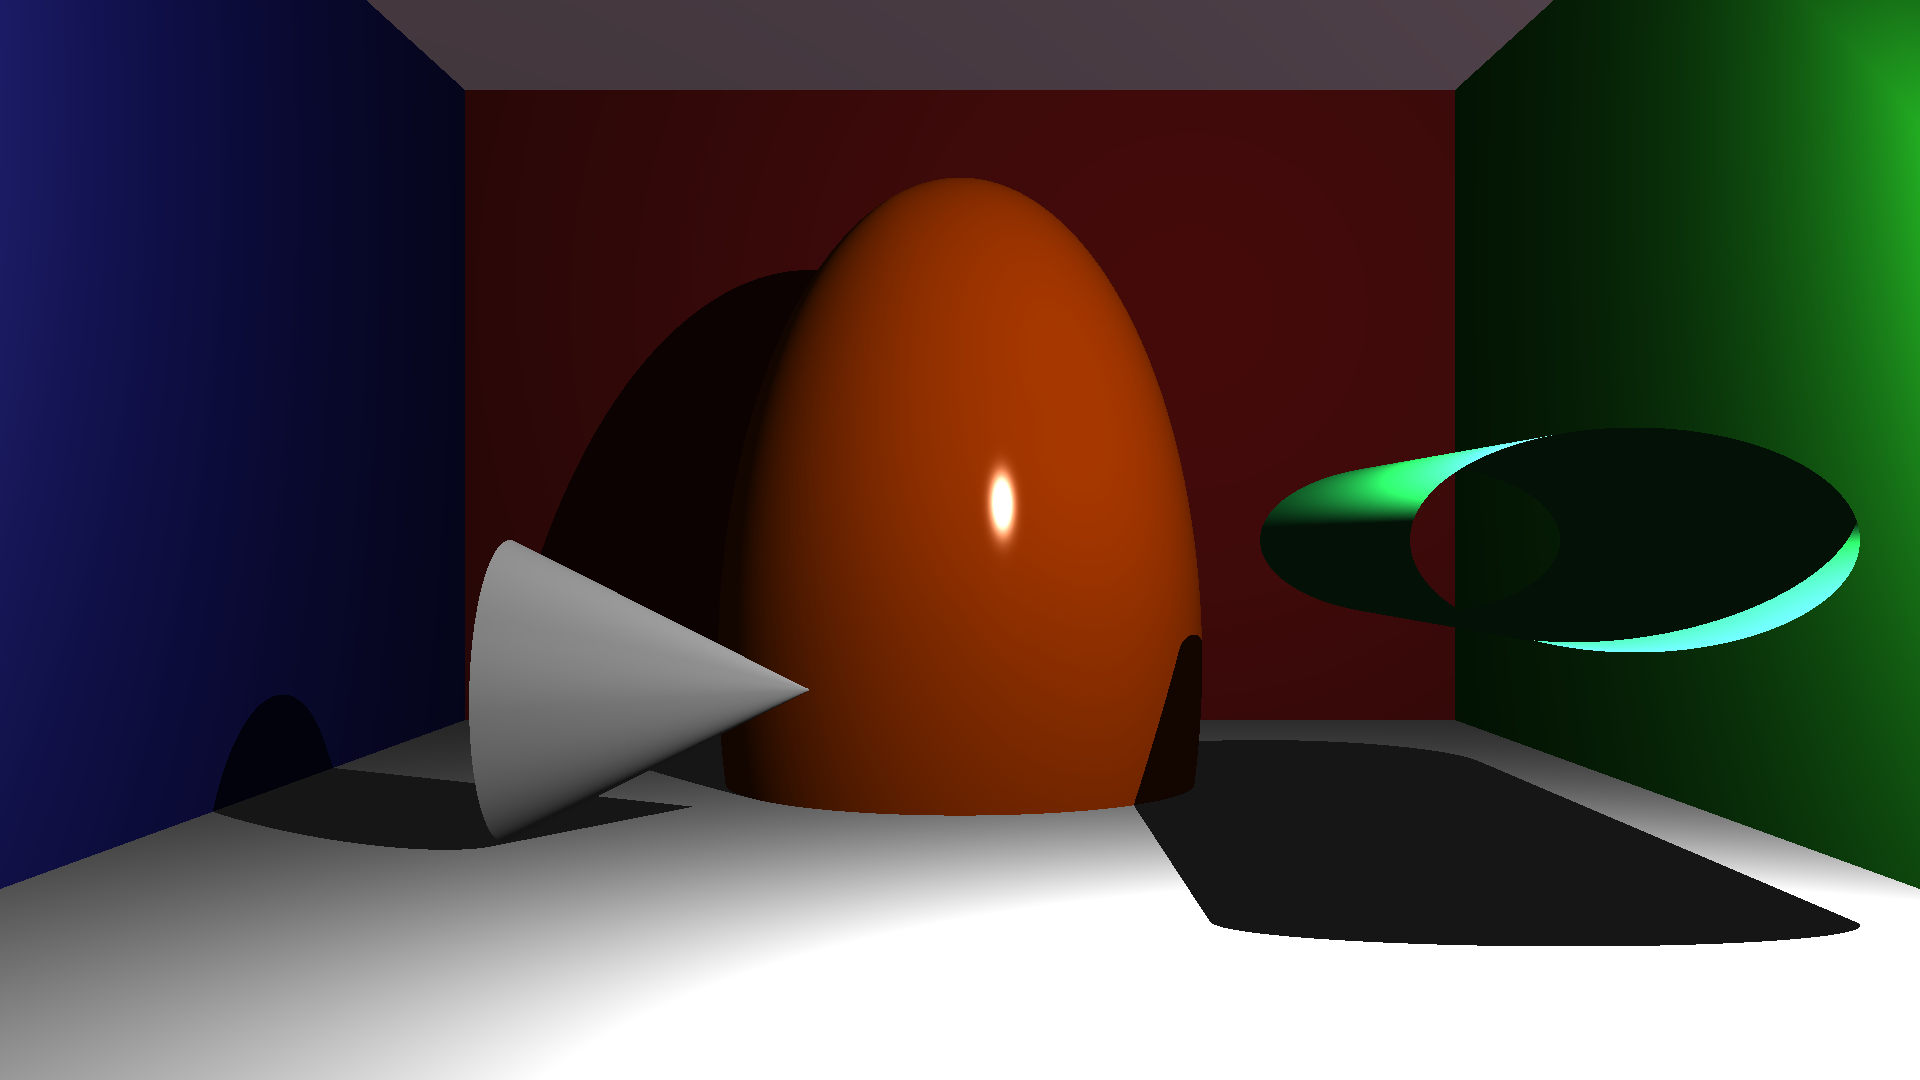
\includegraphics[width=0.45\textwidth]{chapters/ch3/img/complexity/3.png}}

\subfigure{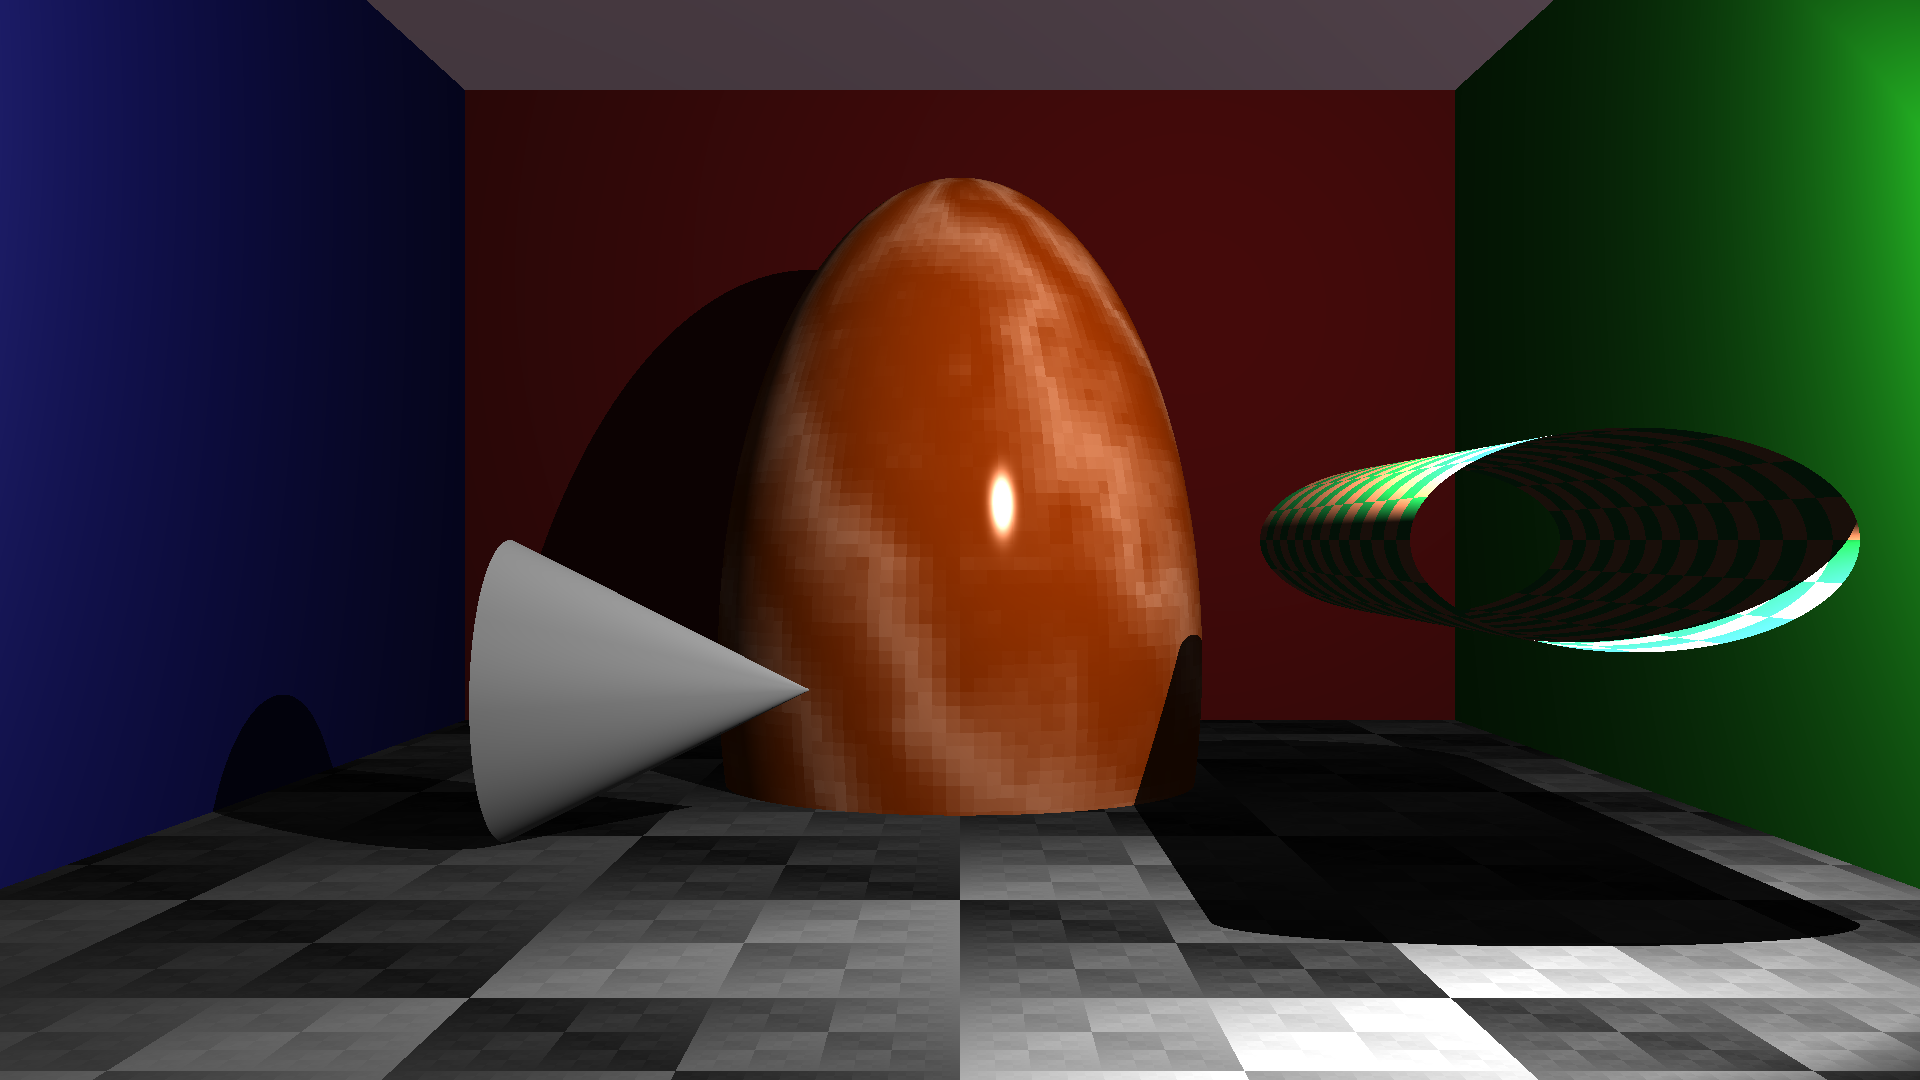
\includegraphics[width=0.45\textwidth]{chapters/ch3/img/complexity/4.png}}
\subfigure{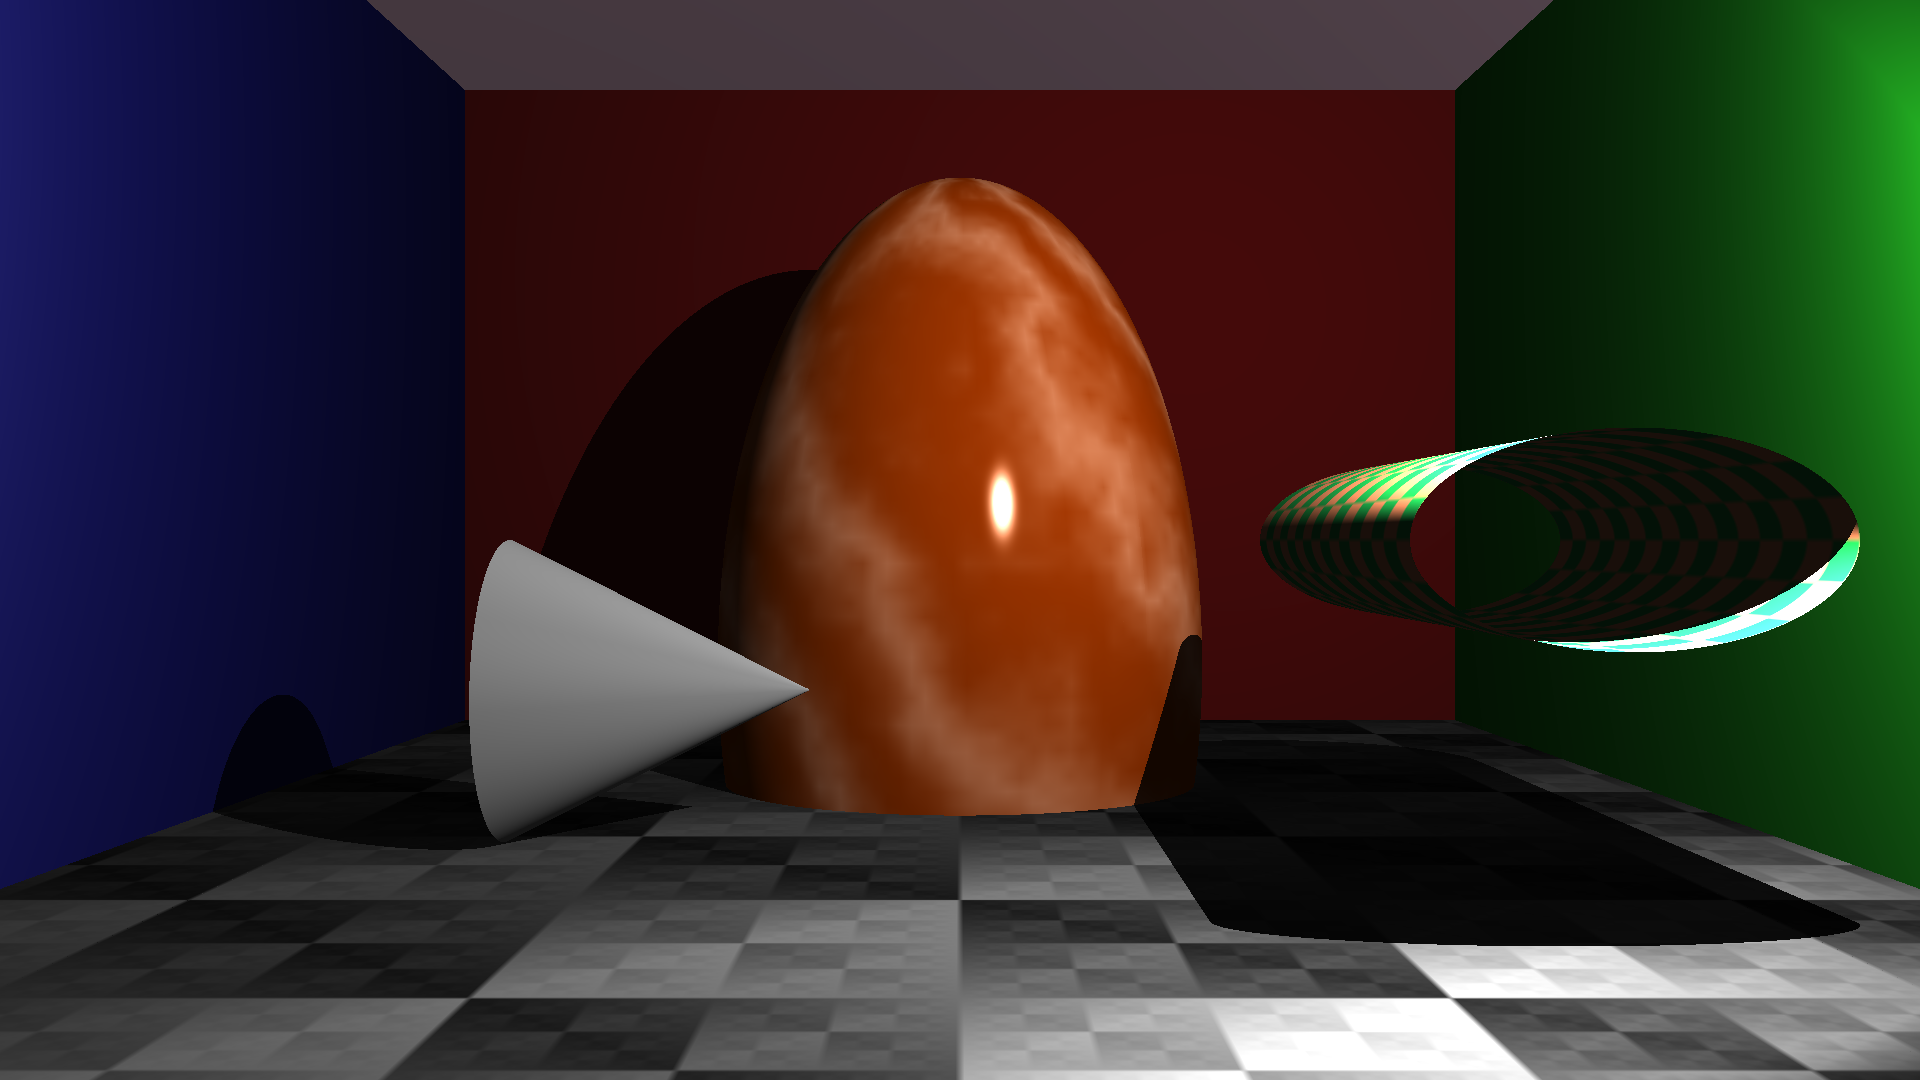
\includegraphics[width=0.45\textwidth]{chapters/ch3/img/complexity/5.png}}

\subfigure{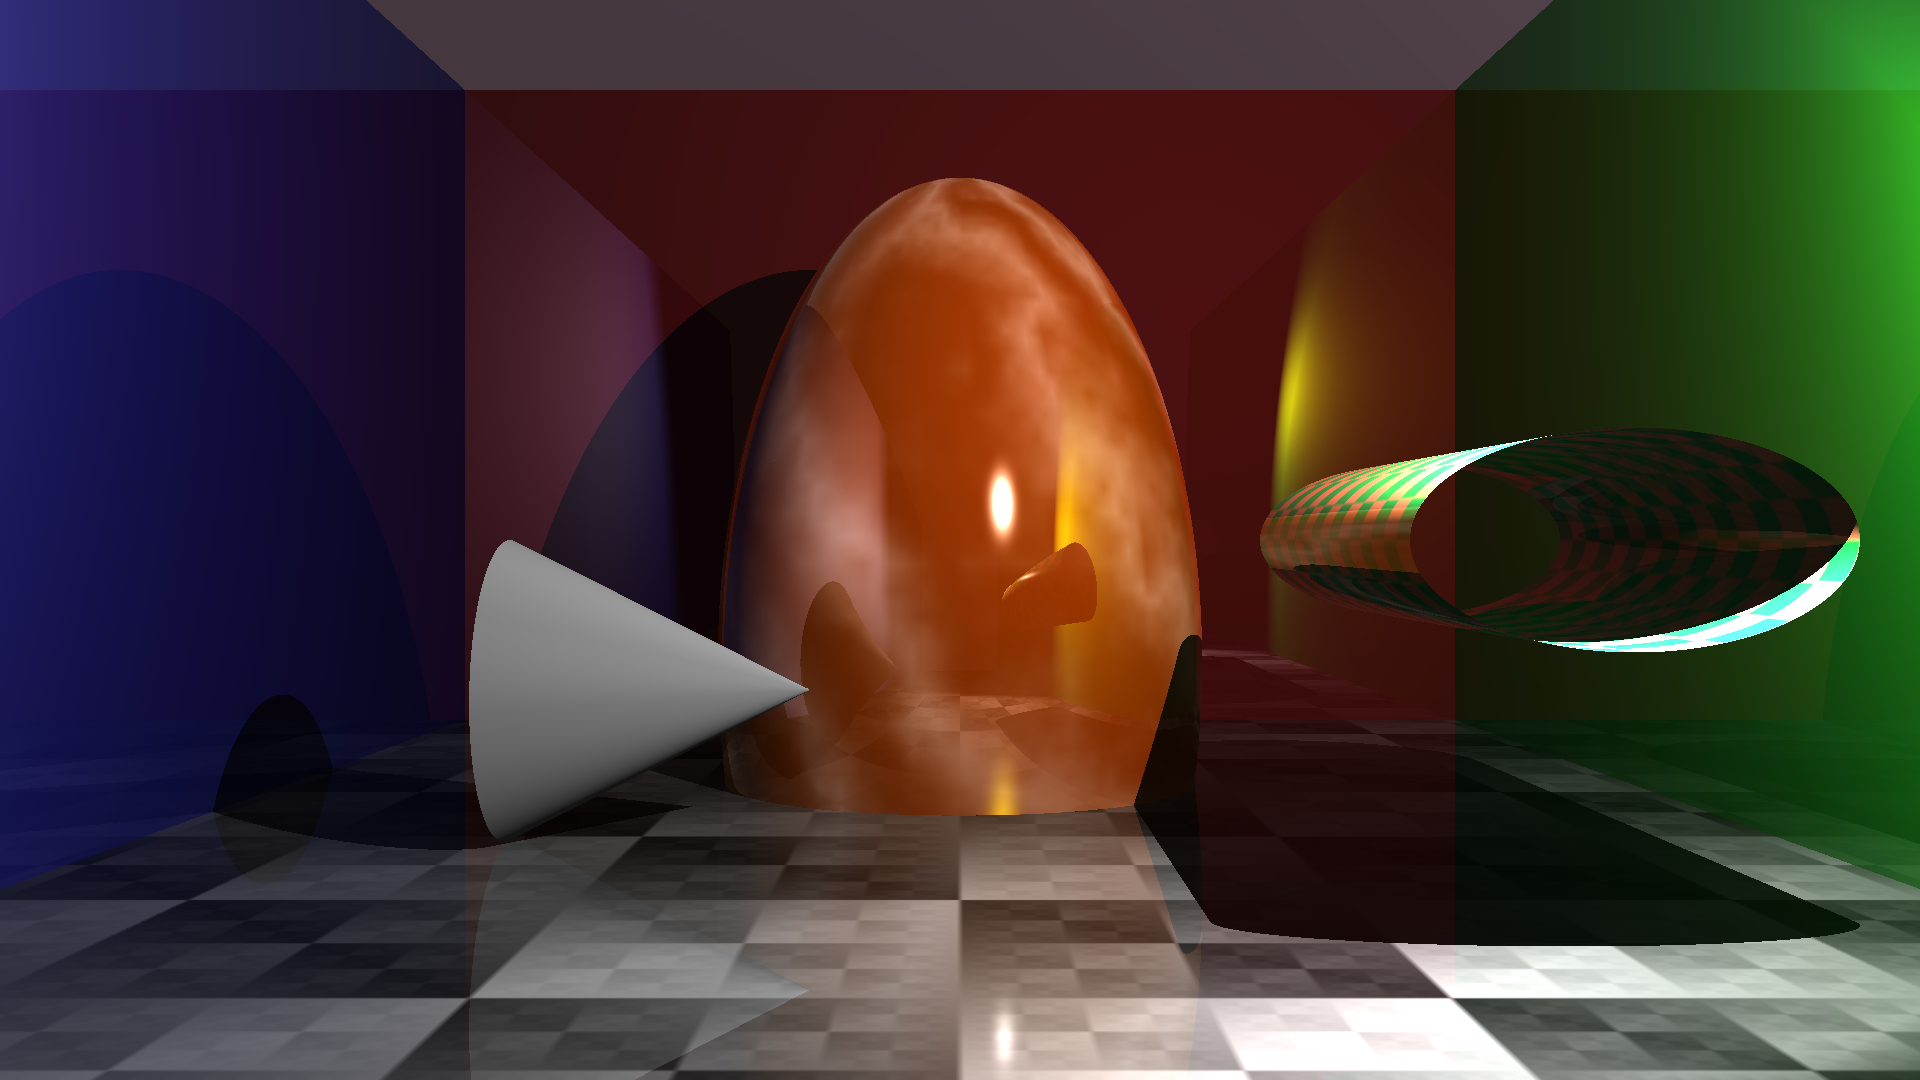
\includegraphics[width=0.45\textwidth]{chapters/ch3/img/complexity/6.png}}
\subfigure{\includegraphics[width=0.45\textwidth]{chapters/ch3/img/complexity/7.png}}

\subfigure{\includegraphics[width=0.45\textwidth]{chapters/ch3/img/complexity/8.png}}
\subfigure{\includegraphics[width=0.45\textwidth]{chapters/ch3/img/complexity/9.png}}


\caption[Wpływ konfiguracji na poziom komplikacji generowanego obrazu]{Wpływ konfiguracji na poziom komplikacji generowanego obrazu. Umożliwienie generowania cieni, a następnie włączenie obliczeń związanych z tworzeniem odbić na~powierzchniach najbardziej wpływają na realizm przedstawionej sceny.}
\label{ch3:img:complexity}
\end{figure}





\section{Implementacja modułu \textsc{ViRay} w układzie FPGA}
Zaprezentowany w poprzednim podrozdziale moduł \textsc{ViRay} jest w pełni funkcjonalny w momencie, gdy zostanie zaimplementowany w układzie FPGA oraz zajdą jednocześnie dwa warunki:
\begin{enumerate}
\item Będzie istniała możliwość dostarczenia do niego poprawnych danych opisujących scenę, która ma zostać wygenerowana.
\item Efekty pracy modułu, czyli finalne ramki obrazu, będą wizualnie weryfikowalne.
\end{enumerate}
Na podstawie tychże wytycznych został zaprojektowany pełen system przetwarzania danych, którego uproszczona wersja schematu blokowego została przedstawiona na schemacie~\ref{ch3:img:block_design}.

Za kontrolę działania omawianego systemu oraz dostarczenie poprawnych danych do \textsc{ViRay}'a odpowiada program w języku C++ wykonywany przez mikrokontroler \texttt{Microblaze}. Został on skonfigurowany w taki sposób aby mógł wykonywać sprzętowo, a nie poprzez emulację, wszystkie operacje zmiennoprzecinkowe pojedynczej precyzji. Dodatkowo jego pamięć na dane oraz instrukcje została rozszerzona do 256~kB każda i nie korzysta on z pamięci podręcznej. Do dyspozycji mikrokontrolera zostały oddane również dodatkowe moduły jak:
\begin{itemize}
\item \texttt{UART}, dzięki któremu możliwe jest odbieranie i wysyłanie komunikatów tekstowych podawanych przez wyjście/wejście standardowe.
\item Licznik czasu pozwalający przeprowadzić diagnostykę czasu wykonania operacji.
\item \texttt{GPIO}, które w przypadku tego konkretnego systemu daje informacje na temat statusu wciśnięcia 5 przycisków zlokalizowanych w prawym dolnym rogu płytki KCU116.
\end{itemize}
Dzięki obecności kontrolera pamięci DDR4 \texttt{Microblaze}~(oraz pozostałe moduły) jest w stanie odwoływać się do puli zewnętrznej względem układu FPGA pamięci RAM, w której mogą być przechowywane większe porcje informacji takie jak finalny obraz wygenerowany przez \textsc{ViRay}.

Obraz ten jest pobierany w trybie ciągłym z pominięciem udziału mikrokontrolera za~pomocą modułu \texttt{VDMA}~(ang.~\textit{Video Direct Memory Access}, bezpośredni dostęp do pamięci wideo)\footnote{Rola mikrokontrolera w tym konkretnym zadaniu sprowadza się jedynie do skonfigurowania parametrów \texttt{VDMA} oraz uruchomienia jego działania.}, synchronizowany względem zegara wynikającego z docelowego formatu~(ten zadany jest przez rozdzielczość aktywnego rozmiaru ramki oraz częstotliwość odświeżania obrazu) a następnie podany na zewnątrz układu FPGA~(\texttt{VTC}, ang.~\textit{Video Timing Controller}; \texttt{Video Out}).

Przetworzone w zaprezentowany sposób dane wizualne trafiają na wejście peryferyjnego układu \texttt{ADV7511} znajdującego się na płytce ewaluacyjnej KCU116, a którego zadaniem jest translacja otrzymanych danych, wedle ustalonych przez użytkownika parametrów pracy, do informacji zgodnej ze standardem HDMI, dzięki czemu finalny obraz może być zaobserwowany po podłączeniu monitora do dostępnego wyjścia obrazu. Parametry pracy układu \texttt{ADV7511}~\cite{ADV7511} muszą zostać ustalone przez \texttt{Microblaze} za pośrednictwem szeregowej szyny transmisji danych \texttt{IIC}~\cite{IIC}.

Z układem \texttt{ADV7511} będącym częścią płytki ewaluacyjnej KCU116 wiąże się obecność dyrektywy \texttt{PIXEL\_COLOR\_CONVERSION\_ENABLE} w finalnej wersji \textsc{ViRay}'a. Konstruktorzy tejże płytki postanowili dokonać redukcji możliwych do wykorzystania linii sygnałowych~\cite{KCU116_UG} wchodzących do układu \texttt{ADV7511} z 36 do 18\footnote{Podane ograniczenie nie występuje w płytce VC707.}. W efekcie w jednym cyklu zegara możliwe jest przesłanie do 18 bitów danych, jednak pełna informacja o kolorze wymaga szyny o szerokości co najmniej $3\cdot 8~\mathrm{b}=24~\mathrm{b}$. Definicja \texttt{PIXEL\_COLOR\_CONVERSION\_ENABLE} redukuje to wymaganie do 16 bitów~(32-bitowa wartość reprezentująca kolor piksela zostaje obcięta do jej 16 najmłodszych bitów, gdyż najstarsze bity nie niosą użytecznej informacji), a brakujące wartości \texttt{B}/\texttt{R} pikseli zostają w pewnym zakresie zrekonstruowane przez układ \texttt{ADV7511}\footnote{Artefakty mogą się pojawiać na kontrastowych krawędziach między obiektami.}.


\begin{landscape}
\addimage{chapters/ch3/img/BLOCK_DESIGN.png}{scale=0.375}{Uproszczony schemat blokowy pełnego systemu przetwarzania danych wykorzystujący stworzony moduł do śledzenia promieni \textsc{ViRay}}{Uproszczony schemat blokowy pełnego systemu przetwarzania danych wykorzystujący stworzony moduł do śledzenia promieni \textsc{ViRay}}{ch3:img:block_design}
\end{landscape}

Stworzony system wykorzystuje 5 głównych sygnałów zegarowych:
\begin{enumerate}
\item Systemowy zegar o częstotliwości 300~MHz, który jest podstawą działania kontrolera pamięci DDR4.
\item Zegar o częstotliwości 333,25~MHz, wytwarzany domyślnie przez kontroler pamięci i~wykorzystywany jako baza do wygenerowania pozostałych częstotliwości.
\item Zegar 160~MHz, który wpływa na szybkość działania i komunikacji większości modułów~(w szczególności \texttt{Microblaze} oraz \texttt{VDMA}). 

Zbadano, iż taka częstotliwość pracy mikrokontrolera jest wystarczająca do obsługi działania \textsc{ViRay}'a w czasie rzeczywistym tzn. czas potrzebny na zaktualizowanie informacji o scenie jest krótszy niż czas generowania obrazu.

\item Główny moduł \textsc{ViRay} pracuje z częstotliwością 320~MHz.

Domyślnie kod \textsc{ViRay}'a jest poddawany syntezie HLS z uwzględnieniem zegara o okresie~3,3~ns~(ok.~303~MHz). Mimo to, moduł ten może zostać z powodzeniem zaimplementowany, gdy częstotliwość jego pracy wynosi~320~MHz. Dzięki temu, teoretycznie wyznaczony czas wygenerowania pełnej klatki maleje o 2,93~ms i wynosi 52,4~ms, dając ok. 19 pełnych klatek obrazu 1920~x~1080 na sekundę. Liczby te można również przedstawić w innej powszechnie spotykanej postaci, mówiącej o tym, ile milionów promieni \textsc{ViRay} jest w stanie przetworzyć w ciągu sekundy~(\texttt{RAYTRACING\_DEPTH = 2} daje 4 promienie na 1 piksel obrazu):
\begin{equation}
4\cdot\frac{1920\cdot 1080}{52,4~\mathrm{ms}}=158,29\cdot 10^6\ \mathrm{\frac{1}{s}}
\end{equation}

Co ciekawe, jeśli \textsc{ViRay} zostanie poddany syntezie Vivado HLS bezpośrednio dla częstotliwości 320~MHz, stworzonego w ten sposób modułu nie da się zaimplementować w układzie FPGA z częstotliwością pracy równą 320~MHz.

\item Zegar synchronizujący dane obrazu o częstotliwości 148,5~MHz.

\textsc{ViRay} został skonfigurowany domyślnie w taki sposób, by generować obrazy o rozdzielczości 1920~x~1080 pikseli. Jednakże ramka obrazu HDMI poza danymi pikseli zawiera również dane dodatkowe~(w tym synchronizacyjne) dołączane do obrazu przez \texttt{Video Out}, w efekcie pełna ramka obrazu w podanej częstotliwości składa się z 2200 poziomych oraz 1125 pionowych linii\footnote{Ilość dodatkowych linii zależy od przyjętej rozdzielczości aktywnego obrazu i można je sprawdzić dla popularnych częstotliwości w oknie konfiguracyjnym modułu \texttt{Video Timing Controller}.}. Chcąc zapewnić częstotliwość odświeżania obrazu równą 60~Hz zegar synchronizacyjny musi mieć wartość:
\begin{equation*}
2200\cdot 1125\cdot 60\ \mathrm{Hz} = 148,5\ \mathrm{MHz}
\end{equation*}
\end{enumerate}
Syntezę pełnego systemu przeprowadzono z użyciem strategi \texttt{Vivado Synthesis Defaults}, a do implementacji \texttt{Performance\_ExplorePostRoutePhysOpt}~(z uwagi na podejmowane przez Vivado w tym przypadku próby optymalizacji struktury, w celu umożliwienia osiągnięcia wysokich częstotliwości pracy). W tabeli~\ref{ch3:tab:implementation_util} przedstawione zostały parametry charakteryzujące cały system po implementacji oraz utylizację zasobów przez \textsc{ViRay} po syntezie do reprezentacji za pomocą netlisty.

\begin{table}[H]
\centering
\caption[Wykorzystanie zasobów sprzętowych układu KCU116 przez zaprojektowany system przetwarzania danych]{Wykorzystanie zasobów sprzętowych układu KCU116 przez zaprojektowany system przetwarzania danych. Środkowy wiersz dotyczy pełnego systemu ze wszystkimi modułami po pomyślnej implementacji, zaś dolny samego modułu \textsc{ViRay} po syntezie do postaci netlisty. Raportowane po syntezie wykorzystanie zasobów przez \textsc{ViRay} jest znacznie niższe niż sugerują to estymowane wartości podawane przez Vivado HLS}
\label{ch3:tab:implementation_util}
\begin{tabular}{|r|c|c|c|c|c|c|}
\hline
\multicolumn{1}{|l|}{} & \textbf{BRAM}                                            & \textbf{DSP}                                             & \textbf{FF}                                                 & \textbf{LUT}                                                & \textbf{\begin{tabular}[c]{@{}c@{}}WNS \\ {[}ns{]}\end{tabular}} & \textbf{\begin{tabular}[c]{@{}c@{}}WHS \\ {[}ns{]}\end{tabular}} \\ \hline
\texttt{System}        & \begin{tabular}[c]{@{}c@{}}430\\ (44,79\%)\end{tabular} & \begin{tabular}[c]{@{}c@{}}919\\ (50,38\%)\end{tabular} & \begin{tabular}[c]{@{}c@{}}238201\\ (54,90\%)\end{tabular} & \begin{tabular}[c]{@{}c@{}}153922\\ (70,94\%)\end{tabular} & 0,032                                                            & 0,006                                                            \\ \hline\hline
\texttt{ViRay}         & \begin{tabular}[c]{@{}c@{}}232\\ (24,17\%)\end{tabular} & \begin{tabular}[c]{@{}c@{}}911\\ (49,95\%)\end{tabular} & \begin{tabular}[c]{@{}c@{}}194557\\ (44,84\%)\end{tabular} & \begin{tabular}[c]{@{}c@{}}130077\\ (59,95\%)\end{tabular} & -                                                                & -                                                                \\ \hline
\end{tabular}
\end{table}

Pierwszą rzeczą, którą należy zauważyć jest to, iż cały system przetwarzania, zawierający oprócz \textsc{ViRay}'a jeszcze wiele innych modułów, wykorzystuje mniejszą ilość FF oraz LUT niż sam \textsc{ViRay} po syntezie HLS~(tabela~\ref{ch3:tab:viray_util}). Dzieje się tak dlatego, iż Vivado HLS dokonuje estymacji wykorzystania elementów układu FPGA w przypadku najbardziej pesymistycznym. Procesy, które zachodzą w wyniku syntezy modułów do postaci netlisty oraz wywołana kolejno implementacja dokonują wielu różnych optymalizacji logiki, które zależą od wybranych strategii. Ten sam projekt zaimplementowany za pomocą innej strategii da~inne wyniki. W szczególności narzędzie mogłoby nie być w stanie zapewnić by nie występowały naruszenia~(WNS/WHS stałyby się ujemne), albo wręcz przeciwnie stworzona struktura byłaby na tyle optymalna, iż możliwe byłoby podniesienie częstotliwości zegara. Z uwagi na wysoki poziom komplikacji projektu oraz mnogość dostępnych parametrów syntezy i implementacji poszukiwanie bezwzględnie najlepszych ustawień byłoby czasochłonne i w gruncie rzeczy nieuzasadnione\footnote{Najważniejszym zadaniem na tym etapie było zapewnienie poprawności działania całego systemu. Błędy popełnione w projekcie schematu blokowego skutkują niepoprawnym działaniem systemu lub jego części i są trudno wykrywalne, czego doświadczono dodając funkcjonalność związaną z transmisją obrazu. Na~komputerze z procesorem Intel Core i5 4690K oraz 16~GB pamięci operacyjnej przeprowadzenie syntezy oraz implementacji trwa niemal 6 godzin, co w znacznym stopniu wpływa na produktywność i szybkość wdrażania wszelkich poprawek. }.

Całkowita estymowana moc energii elektrycznej pobieranej przez KCU116 w trakcie pracy przedstawionego systemu wynosi 13,444~W z czego 95\% to moc dynamiczna, czyli~związana z przełączaniem stanu tranzystorów. Wartość ta w porównaniu z mocą potrzebną do~zasilenia procesorów współczesnych komputerów osobistych jest niewielka\footnote{Oszacowanie mocy energii elektrycznej pobieranej przez procesor nie jest łatwym zadaniem. Producenci posługują się tzw.~\textit{współczynnikiem~TDP}~(ang.~\textit{Thermal Design Power}), który informuje jedynie o średniej mocy promieniowania termicznego emitowanego przez procesor w określonych przez producenta warunkach.}, zwłaszcza gdy weźmie się pod uwagę uzyskiwany przyrost wydajności rzędu~$10^3$.

\section{Oprogramowanie mikrokontrolera}
Zaletą procesora \texttt{Microblaze} jest nie tylko elastyczność pod względem tworzenia konfiguracji, ale przede wszystkim fakt, iż można go programować tak jak zwykły procesor za~pomocą języka C/C++. Fakt ten jest intensywnie wykorzystywany przez napisany sterownik, dzięki któremu następuje nawiązanie poprawnej komunikacji ze wszystkimi modułami znajdującymi się w projekcie, przygotowanie danych oraz obsługa zdarzeń\footnote{Pliki tego projektu znajdują się w repozytorium \url{https://bitbucket.org/rtMasters/ffcore_uc_kintex/commits/branch/KCU116_VIRAY_HDMI_FULL_SYSTEM}. Do poprawnego działania są również wymagane pliki \textsc{ViRay}'a z defininicją \texttt{UC\_OPERATION}.}.

Najważniejszym elementem sterownika decydującym o pracy \textsc{ViRay}'a jest obiekt klasy \texttt{MyWorld}, która dziedziczy po klasie \texttt{WorldDescription}. Zadaniem klasy bazowej jest ustanowienie kontraktu między sterownikiem a modułem śledzenia promieni dotyczący tego, gdzie w przestrzeni adresowej znajdują się dane, które będą interpretowane przez \textsc{ViRay} jako odpowiednie dane opisujące scenę~(tj.~kamera, obiekty, światła, materiały, tekstury) oraz jaki adres odpowiadać ma początkowi danych opisujących finalne piksele obrazu. W~tym~celu wykorzystywany jest sterownik generowany automatycznie przez Vivado HLS, udostępniający funkcje odpowiedzialne m.~in.~za~przypisanie odpowiednich adresów, które będą wykorzystane przez porty, dla których zastosowano interfejs \texttt{AXI4-Lite}. 

Ponadto klasa \texttt{WorldDescription} udostępnia klasie potomnej zestaw narzędzi pozwalających w łatwy sposób definiować poszczególne elementy związane z konfiguracją m.~in.~świateł, obiektów i ich materiałów. Dzięki temu użytkownik w intuicyjny sposób może dokonywać zmian wymaganych w danej chwili parametrów i nie jest zmuszony martwić się osobiście tym, w jaki sposób dane dotyczące obiektów należy upakować w pamięci, gdyż dzieje się to automatycznie.

\begin{lstlisting}[caption=Przykład konfiguracji obiektu \texttt{floor}. Za pomocą odpowiednich funkcji \texttt{Set*()} można dokonać zmiany wartości dowolnych parametrów interpretowanych przez \textsc{ViRay()}]
floor.SetObjType(ObjectType::DISK);
floor.GetTransformHandler().SetTranslation(vec3(0.0f, -2.0f, 0.0f));
floor.GetTransformHandler().SetOrientation(vec3(0.0f, 1.0f, 0.0f));
floor.GetTransformHandler().SetScale(vec3(20.0f));

floor.GetMaterialHandler().SetPrimaryDiffuseColor(vec3(0.9f));
floor.GetMaterialHandler().SetSecondaryDiffuseColor(vec3(0.1f));
floor.GetMaterialHandler().SetTextureScale(vec3(6.0f));
\end{lstlisting}

Dane tekstur generowane są za pomocą instancji klasy typu \texttt{CTextureHelper} znajdującej się wewnątrz \texttt{WorldDescription}, która umożliwia tworzenie tekstur na podstawie 5 dostępnych algorytmów~(rysunek~\ref{ch3:img:textures}) oraz przypisanie jej do obiektów z żądanym trybem mapowania - 4 z nich~(\texttt{XOR}, \texttt{CHECKERBOARD}, \texttt{MARBLE} oraz \texttt{WOOD}) generują mapy szarości, na podstawie których dokonywane jest mieszanie między dwoma kolorami wybranymi przez użytkownika~(\texttt{PrimaryDiffuseColor}, \texttt{SecondaryDiffuseColor}) zaś ostatnia \texttt{RGB\_DOTS} tworzy prostą mapę bitową, w której kolejne piksele mają kolory podstawowe: czerwony, zielony, niebieski.
\addimage{chapters/ch3/img/textures.png}{width=1.0\textwidth}{Typy tekstur mogące zostać wygenerowane przez sterownik. Od lewej do prawej z góry na dół: \texttt{XOR}, \texttt{CHECKERBOARD}, \texttt{RGB\_DOTS}, \texttt{MARBLE}, \texttt{WOOD}. Wygląd tekstur może być konfigurowany za pomocą opcjonalnych parametrów~(dotyczy zwłaszcza dwóch ostatnich przykładów, których wygląd zależy od parametrów rozkładów liczb pseudolosowych)}{Typy tekstur mogące zostać wygenerowane przez sterownik}{ch3:img:textures}

W domyślnej konfiguracji po
\begin{itemize}
\item zapisaniu poprzez magistralę \texttt{IIC} konfiguracji układu \texttt{ADV7511} dostosowanej do formatu przesyłanych danych wizualnych,
\item ustawieniu parametrów i uruchomieniu transferu danych za pomocą \texttt{VDMA},
\item zapisaniu danych dotyczących generowanej sceny trójwymiarowej,
\end{itemize}
\textsc{ViRay} zostaje uruchomiony w trybie samopowtarzalnym. Dzieje się to za pomocą sekwencji wywołań funkcji \texttt{XViraymain\_EnableAutoRestart()} oraz \texttt{XViraymain\_Start()}, a~sam~sterownik przechodzi do nieskończonej pętli głównej, w której dokonuje aktualizacji sceny. Aktualizacja ta wynika:
\begin{itemize}
\item z czasu $\Delta t$, który upłynął między kolejnymi iteracjami pętli, a który jest liczony dzięki obecności w systemie licznika cykli zegara,
\item możliwej akcji użytkownika, który mógł dokonać naciśnięcia przycisków obsługiwanych przez moduł \texttt{GPIO}.
\end{itemize}

W przykładowej scenie, która jest realizowana przez kod znajdujący się w repozytorium, upływ czasu pozwala dokonać zmian położenia źródła światła, przesuwać teksturę podłoża czy zmieniać rozmiary obiektów zgodnie z przyjętym algorytmem. Naciśnięcie przycisków na płytce KCU116 jest zaś traktowane, jako chęć zmiany położenia lub orientacji obserwatora w przestrzeni pozwalając ustawić kamerę w pożądanym miejscu. Poniższe ilustracje przedstawiają pracę opisywanego systemu.

\begin{figure}[H]
\centering
\subfigure{\includegraphics[width=0.9\textwidth]{chapters/ch3/img/system/1.jpg}}
\subfigure{\includegraphics[width=0.9\textwidth]{chapters/ch3/img/system/2.jpg}}
\caption[Wygenerowane w czasie rzeczywistym klatki animacji otrzymane dzięki wykorzystaniu techniki śledzenia promieni akcelerowanej przez stworzony z użyciem Vivado HLS moduł \textsc{ViRay}]{Wygenerowane w czasie rzeczywistym klatki animacji otrzymane dzięki wykorzystaniu techniki śledzenia promieni akcelerowanej przez stworzony z użyciem Vivado HLS moduł \textsc{ViRay}. Finalna wersja systemu pozwala generować interaktywne obrazy o rozdzielczości 1920~x~1080 pikseli ze stałą szybkością 19 klatek na sekundę}
\label{ch3:img:system}
\end{figure}

%%%%%%%%%%%%%%%%%%%%%%%%%%%%%%%%%%%%%%%%%%%%%%%%%%%%%%%%%%%%%%%%%%%%%%%%%%%%%%%%%%%%%%%%%%%%%%%%%%%%%%%%%%%%%%%%%%%%%%


\section*{Podsumowanie}
\addcontentsline{toc}{section}{Podsumowanie}
Przedstawiony rozdział stanowi najważniejszą część prezentowanej pracy. Wykorzystując wiedzę teoretyczną zebraną w dwóch poprzednich rozdziałach podjęte zostały próby stworzenia systemu, którego celem byłaby akceleracja tworzenia obrazów metodą śledzenia promieni. Okazało się, iż na obecnym etapie rozwoju Vivado~HLS nie jest możliwe stworzenie rozsądnego pod względem funkcjonalności, szybkości oraz użytych zasobów rozwiązania opartego o sieć wyspecjalizowanych procesorów arytmetycznych. 

Z powodzeniem natomiast zaprojektowano moduł spełniający postawione przed projektem wymagania i charakteryzujący się tym, że jego funkcjonalność jest stała i kontrolowana poprzez skończony zbiór ściśle określonych parametrów wpływających na odbiór obiektów znajdujących się w generowanej scenie. W ten sposób Vivado~HLS wiedząc, w jaki konkretny sposób dane są przetwarzane na kolejnych etapach, było w stanie zastosować odpowiednie optymalizacje. Efekt końcowy wymagał włożenia wiele wysiłku i poczynienia rozmaitych kompromisów opisanych w tym rozdziale po to, aby uzyskać moduł o optymalnej funkcjonalności, który na dodatek mógłby zostać zaimplementowany w układzie FPGA.

Kluczowym czynnikiem wpływającym na skomplikowanie akceleratora jest reprezentacja danych, na których wykonywane są operacje. \textsc{ViRay} domyślnie wykorzystuje typ \texttt{float} chociaż istnieje przypuszczenie~(znajdujące potwierdzenie w cytowanej literaturze~\cite{RPU}), iż gdyby tylko Vivado HLS pozwalało stosować typy zmiennopozycyjne o dowolnej ilości bitów, \textsc{ViRay} mógłby być bardziej funkcjonalny przy jednoczesnym zachowaniu wystarczającej precyzji obliczeń.

Ponadto, gdyby nie dostęp do najnowocześniejszego układu FPGA śledzenie promieni rozproszonych nie byłoby możliwe, a przez to obrazy nie różniłyby się znacząco od tych, które można stworzyć na drodze rasteryzacji. Mimo tego i tak trzeba było wykonać wiele ustępstw w stosunku do funkcjonalności~(m.~in. ograniczyć swobodę umieszczania obiektów w przestrzeni) oraz nie uniknięto problemów, które wynikały z naprawienia drobnych błędów w algorytmie np.:
\begin{itemize}
\item poprawienie obliczania reflektancji materiałów przewodzących wymusiło zmniejszenie częstotliwości zegara modułu z 335~MHz do 320~MHz,
\item implementacja modelu BRDF Orena-Nayara do samego końca nie była pewna w finalnej wersji \textsc{ViRay}'a, gdyż dodanie odpowiedniego kodu związanego z obliczeniem właściwego współczynnika całkowicie uniemożliwiało implementację w układzie FPGA nawet dla niskich częstotliwości pracy.
\end{itemize}

Mimo wielu napotkanych przeciwności, finalny moduł \textsc{ViRay} został zintegrowany w~pełnym systemie przetwarzania danych, kontrolowanym przez mikroprocesor \texttt{Microblaze}. Wyniki działania \textsc{ViRay}'a w postaci animacji są generowane z szybkością 19~klatek obrazu na~sekundę w rozdzielczości 1920~x~1080~pikseli i można je zobaczyć podłączając monitor lub telewizor do źródła HDMI znajdującego się na wykorzystanej płytce ewaluacyjnej KCU116.

\begin{center}
$*\qquad *\qquad *$
\end{center}

Stworzony moduł stanowi tylko bardzo uproszczoną implementację śledzenia promieni, którą można poddawać dalszym modyfikacjom. 

Zgodnie z założeniami, obiekty w scenie opisane są poprzez odpowiednie równania - różne dla każdego obiektu. Sprawia to, że funkcje badające przecięcia promieni z obiektami wymagają dużych ilości elementów logicznych do ich implementacji. Pod tym względem, świat złożony z trójkątów jest znacznie bardziej atrakcyjny, gdyż wystarczyłoby jedynie sprawdzać przecięcia z jednym typem obiektów. W takim przypadku należałoby stworzyć dodatkowo funkcję/moduł przyspieszający testy przecięcia, gdyż poddane triangulacji obiekty mogą składać się z tysięcy trójkątów. Taka funkcjonalność musiałaby nie tylko błyskawicznie dokonywać testów geometrii, ale również zarządzać tysiącami obiektów, których dane nie mogą znaleźć się w całości w pamięci blokowej BRAM układu FPGA. Jak się okazuje, wynika z tego pojawienie się problemów, związanych z użyciem Vivado HLS, podobnych do~tych, które zostały odkryte podczas opracowywania rozwiązania procesorowego.

Ciekawym dodatkiem mógłby być też pośredni zapis kolorów pikseli do zmiennopozycyjnego bufora o znacznie większej dynamice tonalnej~(ang.~\textit{high dynamic range}, HDR) po~to, aby na etapie konwersji do obrazu o niskiej, 8-bitowej, dynamice~(ang.~\textit{low dynamic range}, LDR) móc lepiej odwzorować detale powierzchni i przeciwdziałać przepaleniom kolorów.

Przyglądając się cytowanej literaturze traktującej o budowie kompleksowego rozwiązania przeprowadzającego symulację transportu światła w przestrzeni~\cite{PBRT}\cite{RTFTGU} już w pierwszych rozdziałach prezentowane są podstawy związane z metodą Monte-Carlo, która wykorzystywana jest do implementacji rozkładu promieni w przestrzeni. Koncepcja ta, w niniejszej pracy, ze względu na ograniczone zasoby sprzętowe układów FPGA, została całkowicie pominięta. Wykorzystując metodę Monte-Carlo można m.~in. wygładzać granice między obiektami~(tzw.~\textit{antyaliasing}), symulować skończoną głębię ostrości kamery, dodawać źródła światła o skończonej powierzchni czy umożliwić generowanie rozproszonych odbić kierunkowych. Wadą tej metody jest jednak konieczność rozpatrywania znacznie większej liczby promieni, aby uzyskać kolor danego piksela. Aktualnie powstają nowe technologie oparte o uczenie maszynowe, których celem jest zmniejszenie liczby wymaganych promieni dla osiągnięcia tych samych efektów, co tradycyjnie~\cite{NVIDIA_JENSEN}\cite{NVIDIA_DEMO}. Mimo tych wysiłków, do tej pory wykorzystanie śledzenia promieni w zastosowaniach czasu rzeczywistego pozostaje w sferze badań największych korporacji zajmujących się tym problemem od dekad.

